%TODO : Mein eigenes Verwendetes System beschreiben, genauer, welche verschiedenen Interaktionen hatte ich, etc. Warum habe ich was gemacht, eventuell sogar mit UML Diagrammen arbeiten
%
%Auch weitere Hypoethesen in Sachen präsenz als zusätzliches Kapitel "Signifikanzanalyse" oder so mit hineinbringen. Nur die, die signifikant sind.
%
%Analyse mit Signifikanzniveau von 10% anschauen, damit Ergebnisse schnelller signifikant sind.
%
%Umbenennung von "VR" und "AVATARE" etc.
%
%Nicht alles so kleingliedrig
%
%Auf Verwendung von nicht parametrische Tests achten.
%
%Leseprobe senden!
%Auswertungen nicht als Screenshot sondern als Tabelle
%Gerichtete Hypothese überprüfen, schauen ob der p-Wert halbiert werden kann

%Kennenlernphase KENNENLERNPHASE ABÄNDERN!
\documentclass[a4paper,11pt]{article}%Schriftgröße

\usepackage{booktabs}
\usepackage{multirow}
\usepackage{rotating}
\newcommand\tabrotate[1]{\begin{turn}{90}\rlap{#1}\end{turn}}
\usepackage{varwidth}
\newcommand\tabvarwidth[2][3cm]{\begin{varwidth}[b]{#1}\centering #2\end{varwidth}}
\usepackage{tabularx}
\usepackage{amsmath}
\usepackage{subfig}
\usepackage{enumitem}
\usepackage{pslatex}
\usepackage[T1]{fontenc} 
\usepackage[utf8]{inputenc}
\usepackage[ngerman]{babel}%Veröffentlichungssprache
\usepackage{graphicx}
\usepackage{ragged2e}
\usepackage[format=plain,justification=RaggedRight,singlelinecheck=false,font={small},labelsep=space]{caption}
\usepackage{float}
\usepackage{xcolor}	
\usepackage[a4paper]{geometry}
\usepackage{fancyhdr}
\usepackage[onehalfspacing]{setspace}%Zeilenabstand
\usepackage[onehalfspacing]{setspace}%Zeilenabstand
\usepackage{fancyhdr}
\usepackage[citestyle=authoryear,natbib=true, backend=bibtex, style=alphabetic]{biblatex}
\usepackage{relsize}
%\usepackage[printonlyused, smaller, footnote]{acronym}
\usepackage[printonlyused, smaller]{acronym}
%\usepackage[printonlyused, withpage, smaller, footnote]{acronym}
\renewcommand{\\}{\vspace*{0.5\baselineskip} \newline}
\renewcommand*\MakeUppercase[1]{#1}	
\renewcommand{\familydefault}{\sfdefault}
\geometry{left=3.5cm,right=2.5cm,top=2.4cm,bottom=2cm}%Seitenränder
\pagestyle{fancy}
\renewcommand{\headrulewidth}{0pt}
\renewcommand{\footrulewidth}{0pt}
\fancyhead[R]{\footnotesize{\thepage}}
\fancyhead[L]{\footnotesize{\leftmark}}
\fancyfoot{}
\usepackage[colorlinks,pdfpagelabels,pdfstartview = FitH,bookmarksopen = true,bookmarksnumbered = true,linkcolor = black,urlcolor = black,plainpages = false,hypertexnames = false,citecolor = black] {hyperref}

\addbibresource{bibfile}
\begin{document}
	\begin{titlepage}
		\begin{flushleft}
			\vspace*{-1cm}
 			
\includegraphics[scale=1]{Abbildungen/TH.png}\\
			\vspace*{1cm}
		\end{flushleft}
		\begin{center}

			\noindent
			%Vergleich des Teambuildingerfolgs mittels eines nicht-vollkörpergetracktem- und vollkörpergetracktem Avatars in einer Immersive Virtual Reality anhand einer Escape-Room-Artigen Umgebung. \\
			
%			Vertrauensaufbau einer Teambuildingmaßnahme zwischen eines Hand- und Kopf getracktem Avatar und  eines Hand-, Kopf und Inverskinematisch-simuliertem Torsos getracktem Avatar in einem Shared Virtual Environment anhand einer Escape-Room-Artigen Umgebung. \\
			
%			Auswirkung des Vertrauens auf die Effizienz in einer Teambuildingmaßnahme anhand eines Hand- und Kopfgetracktem und einem Hand-, Kopf und Inverskinematisch-simuliertem Torsos getracktem Avatar ein einem Shared Virtual Environment. //
			
%			Auswirkung von Vertrauen zu Avataren auf die \mbox{Effizienz} in einer Teambuildingmaßnahme in ein einem Shared Virtual Environment.

%Auswirkung des Vertrauens einer Teambuildingmaßnahme anhand eines \glqq{}IK-Avatar\dq{}und einem \glqq{}Non-IK-Avatar\dq{} in einem Shared-Virtual-Environment. \\
%
%Auswirkung des Vertrauens auf die Effizienz einer Teambuildingmaßnahme anhand eines \glqq{}IK-Avatar\dq{}und einem \glqq{}Non-IK-Avatar\dq{} in einem Shared-Virtual-Environment. \\
%
%Welche Avatar-Kondition schafft in meinem Team mehr Vertrauen? Hat dieses geschaffene Vertrauen eine Auswirkung auf die Effizienz meiner Teambuildingmaßnahme? Welche Avatar-Kondition sollte ich also nutzen, um Vertrauen zu schaffen, sodass in einem Team ein effizienteres Arbeiten stattfinden kann?

%Auswirkung von Vertrauen auf die Anfangsphase einer virtuellen Teamgrün
\begin{huge}
%Einfluss des gebildeten Vertrauens von \ac{ik} und \ac{nik} Avataren auf die \textit{Teameffektivität} in einem kurzzeitig zusammenarbeitenden virtuellem Team.
Der Einfluss der Avatar-Darstellung auf das Vertrauen und die Effektivität eines Teams in einem Shared-Virtual-Environment \\
%Einfluss der Vertrauensbildung zwischen \ac{ik} und \ac{nik} Avataren auf die \textit{Teameffektivität} in einem kurzzeitig zusammenarbeitenden virtuellem Team.\\
\end{huge}
\vspace{2cm} 
		 Masterarbeit zur Erlangung des akademischen Grades\\ \vspace{0.5cm} 
		 \textit{Master of Science}\\ \vspace{0.5cm} 
		 im Studiengang Medientechnologie\\
		 an der Fakultät für Informations-, Medien- und Elektrotechnik\\
		 der Technischen Hochschule Köln
		~\\
		~\\
		~\\\vspace{1cm} 
		\noindent\begin{tabular}{ll}
			vorgelegt von: & Hannes Hinrichs \\
			Matrikel-Nr.: &	11121733 \\
			Adresse: & Zülpicher Straße 19 \\
			~ &	50674 Köln \\
			~ &	hannes.hinrichs@web.de \\
			~ & ~ \\
			eingereicht bei: & Prof. Dr. Arnulph Fuhrmann \\
			Zweitgutachter: & Prof. Dr. Stefan Grünvogel
		\end{tabular}	
		~\\
		~\\\vspace{1cm} 
		{\today}
	\end{center}
	\end{titlepage}
	\pagenumbering{Roman}
	\pagestyle{fancy}
	\newpage
\section*{Eidesstattliche Versicherung}\markboth{Eidesstattliche Versicherung}{Eidesstattliche Versicherung}\addcontentsline{toc}{section}{Eidesstattliche Versicherung}
	Ich versichere, die von mir vorgelegte Arbeit selbstständig verfasst zu haben. Alle Stellen, die wörtlich oder sinngemäß aus veröffentlichten oder nicht veröffentlichten Arbeiten anderer oder der Verfasserin/des Verfassers selbst entnommen sind, habe ich als entnommen kenntlich gemacht. Sämtliche Quellen und Hilfsmittel, die ich für die Arbeit benutzt habe, sind angegeben. Die Arbeit hat mit gleichem Inhalt bzw. in wesentlichen Teilen noch keiner anderen Prüfungsbehörde vorgelegen.\\
	~\\
	~\\
	\rule{0.35\textwidth}{0.4pt} \hspace*{3cm} \rule{0.45\textwidth}{0.4pt} \newline
	Ort, Datum	\hspace*{6.3cm}	Rechtsverbindliche Unterschrift
	\newpage
\section*{Kurzfassung}\markboth{Kurzfassung}{Kurzfassung}\addcontentsline{toc}{section}{Kurzfassung}
Das Ziel dieser Arbeit ist es, herauszufinden, ob unterschiedliche Avatar-Darstellungen einen Einfluss auf das gebildete kognitive Vertrauen und die Effektivität eines Teams besitzen. Die erste Frage dabei ist, ob eine invers-kinematische menschenähnliche Repräsentation oder eine abstrakte nicht menschenähnliche Repräsentation wirkungsvoller ist, um Vertrauen in einem neu gegründeten virtuellen Team zu generieren. Die zweite Frage setzt sich damit auseinander, ob sich das durch die unterschiedlichen Repräsentationen gebildete kognitive Vertrauen auf die Effektivität des virtuellen Teams auswirkt. Um diese Fragen zu beantworten, wurde eine quantitative Studie durchgeführt, bei der verschiedene Teilnehmer in einem Drei-Personen-Team eine kollaborative Aufgabe in einem Shared-Virtual-Environment durchführten. Es konnten dabei keine signifikanten Unterschiede der Effektivität zwischen den Teams mit meschenähnlichen und nicht menschenähnlichen Repräsentationen festgestellt werden. Die Ergebnisse der Studie zeigen zudem, dass in den Drei-Personen-Teams signifikant mehr Vertrauen zu nicht menschenähnlichen Avataren aufgebaut wurde sowie, dass bei dieser Avatardarstellung ein signifikanter Zusammenhang zwischen dem gebildeten kognitiven Vertrauen und der Teameffektivität besteht. Dies bedeutet, dass die Simplizität eines nicht menschenähnlichen Avatars in einem neu gegründeten Team in einem Shared-Virtual-Environment wirkungsvoll sein kann, um dort eine vertrauensvolle Arbeitsatmosphäre zu schaffen. 
	
			\paragraph{Stichwörter}
			Virtual-Reality, Vertrauen, Teamgründung, virtuelles Team, Avatar
			
			\paragraph{Datum}
			{\today}
	\newpage
	
\section*{Abstract}\markboth{Abstract}{Abstract}
%\addcontentsline{toc}{section}{Abstract}
The goal of this work is to find out if different avatar representations have an impact on the formed trust and effectiveness of a team. The first question here is whether an inverse-kinematic human-like representation or an abstract non-human-like representation is more effective in generating trust in a newly formed virtual team. The second question addresses whether the trust formed by the different representations influences the effectiveness of the virtual team. To answer these questions, a quantitative study was conducted in which different participants in a three-person team performed a collaborative task in a shared virtual environment. No significant differences in effectiveness were found between the teams. The results of the study also show that in the threeperson team significantly more trust was built with non humanlike avatars. Furthermore, with non-human-like avatars there was a significant relationship between the cognitive trust formed and teameffectiveness. This means that the simplicity of a non-human-like avatar in a newly formed team in a shared virtual environment can be effective in creating a trusting work atmosphere.

	
			\paragraph{Keywords}
			Virtual-Reality, Trust, Team formation, virtual Team, Avatar
			
			\paragraph{Date}
			{\today}
	\newpage
	\tableofcontents
	\newpage

\listoffigures% Abbildungsverzeichnis
\addcontentsline{toc}{section}{Abbildungsverzeichnis}
\newpage
\listoftables% Tabellenverzeichnis
\addcontentsline{toc}{section}{Tabellenverzeichnis}
\newpage
	
\section*{Abkürzungsverzeichnis}\markboth{Abkürzungsverzeichnis}{Abkürzungsverzeichnis}\addcontentsline{toc}{section}{Abkürzungsverzeichnis}
	\begin{acronym}[NIK-T.Lvl.Rounds]
	\acro{hmd}[HMD]{Head-Mounted-Display}
	\acro{sve}[SVE]{Shared-Virtual-Environment}
	\acro{vr}[VR]{Virtual-Reality}
	\acro{ivr}[IVR]{Immersive-Virtual-Reality}
	\acro{ipo}[IPO]{Input-Process-Output}
	\acro{fov}[FOV]{Field-of-View}
	\acro{bip}[BIP]{Break-in-Presence}
	
	\acro{ik}[IK]{Invers-Kinematisch - (Hand-, Kopf und Inverskinematisch-simulierter Torso)}
	\acro{nik}[NIK]{Nicht-Invers-Kinematisch (Hand- und Kopf getrackter Avatar)}
	
	\acro{gt}[GT]{Generelles Vertrauen}
	\acro{gti}[GTI]{Generelles Vertrauen - IK}
	\acro{gtn}[GTN]{Generelles Vertrauen - NIK}
	
	\acro{ct}[CT]{Kognitives Vertrauen}
	\acro{cti}[CTI]{Kognitives Vertrauen - IK}
	\acro{ctn}[CTN]{Kognitives Vertrauen - NIK}
	
	\acro{tc}[TC]{Team-Kommunikation}
	\acro{tci}[TCI]{Team-Kommunikation - IK}
	\acro{tcn}[TCN]{Team-Kommunikation - NIK}
	
	\acro{tRound}[T.Lvl.Rounds]{Erfolgreich abgeschlossene Runden auf Team-Level}
	\acro{tRoundIK}[IK-T.Lvl.Rounds]{Erfolgreiche abgeschlossene Runden auf Team-Level - IK}
	\acro{tRoundNIK}[NIK-T.Lvl.Rounds]{Erfolgreiche abgeschlossene Runden auf Team-Level - NIK}
	
	\acro{te}[TE]{Teameffektivität}
	\acro{tei}[TEI]{Teameffektivität - IK}
	\acro{ten}[TEN]{Teameffektivität - NIK}
	
	\acro{cp}[CP]{Co-Präsenz}
	\acro{cpi}[CPI]{Co-Präsenz - IK}
	\acro{cpn}[CPN]{Co-Präsenz - NIK}
	
	\acro{tlx}[NTLX]{Nasa-TLX}
	\acro{tlxi}[NTLXI]{Nasa-TLX - IK}
	\acro{tlxn}[NTLXN]{Nasa-TLX - NIK}
	
	\acro{teamCog}[T.Lvl.Cog]{Kognitives Vertrauen auf Team-Level}
	\acro{teamCogIK}[IK-T.Lvl.Cog]{Kognitives Vertrauen auf Team-Level - IK}
	\acro{teamCogNIK}[NIK-T.Lvl.Cog]{Kognitives Vertrauen auf Team-Level - NIK}
	
	\acro{teamGen}[T.Lvl.Gen]{Generelles Vertrauen auf Team-Level}
	\acro{teamGenIK}[IK-T.Lvl.Gen]{Generelles Vertrauen auf Team-Level - IK}
	\acro{teamGenNIK}[NIK-T.Lvl.Gen]{Generelles Vertrauen auf Team-Level - NIK}
	
	\acro{scp}[SCP]{Self-Co-Präsenz}
	\acro{scpi}[SCPI]{Self-Co-Präsenz - IK}
	\acro{scpn}[SCPN]{Self-Co-Präsenz - NIK}	
	
	\acro{ocp}[OCP]{Other-Co-Präsenz}
	\acro{ocpi}[OCPI]{Other-Co-Präsenz - IK}
	\acro{ocpn}[OCPN]{Other-Co-Präsenz - NIK}	
	
	\acro{ipq}[IPQ]{Fragebogen des Anstrengungsmaß}
	\acro{ipqi}[IPQI]{Fragebogen des Anstrengungsmaß - IK}
	\acro{ipqn}[IPQN]{Fragebogen des Anstrengungsmaß - NIK}
	
	\acro{tp}[TP]{Telepresence}
	\acro{tpi}[TPI]{Telepresence - IK}
	\acro{tpn}[TPN]{Telepresence - NIK}	
	
	\acro{sp}[SP]{Social-Presence}
	\acro{spi}[SPI]{Social-Presence - IK}
	\acro{spn}[SPN]{Social-Presence - NIK}
	
	\acro{vts}[VT's]{Virtuelle Teams}
%	iktc teamCogIK
%	niktc teamCogNIK
%	tCog teamCog
\end{acronym}

	
	%\newpage
	%\listoftables\addcontentsline{toc}{section}{Tabellenverzeichnis}
	%\newpage
	%\listoffigures\addcontentsline{toc}{section}{Abbildungsverzeichnis}
	\newpage
	\pagenumbering{arabic}
	
%\section{Abgrenzung zu anderen Studien}
%	\begin{itemize}
%	\item{Team besteht aus 3! Personen}
%	\item{Es wird die initiale Anfangsphase eines Teams untersucht}
%	
%	\item{Es wird geschaut, ob das geschaffene Vertrauen eine Auswirkung auf die Team-Effizienz hat}
%	\item{Es wird schaut, mit welcher Kondition ( Self-Avatar vs. non Self-Avatar ) mehr Vertrauen in das Team geschaffen wurde}
%	\item{Es wird geschaut, mit welcher Kondition ( Self-Avatar vs non Self-Avatar ) eine höhere Team-Effizienz wird}
%	\end{itemize}		
	

%Der Titel dieser Masterarbeit lässt sich in 2 Fragestellungen unterteilen :

%Ist die Avatar-Kondition \ac{ik} oder die Avatar-Kondition \ac{nik} effektiver um Vertrauen in einem \ac{sve} zu bilden?
%Falls es auswirkungen gibt :
%Welche Avatar-Kondition sollte man nutzen um frühzeitig Vertrauen zu bilden?
%Warum ist eine Avatar-Kondition effektiver?
%Falls es keine Auswirkungen gibt :
%Weshalb gibt es keine Auswirkungen?
%Was hat der Versuchsaufbau mit den Ergebnissen zu tun?
%

%Wirkt sich das gebildete Vertrauen der verschiedenen Avatar-Konditionen auf die Effektivität eines virtuellen Teams aus?
%Wenn ja : Welche Avatar-Kondition ist effektiver?
%Wie viel effektiver ist eine Avatar-Konditione?
%Wenn nein : Woran liegt es, dass die Teams gleich effektiv sind?

%Was bedeutet das im Allgemeinen für ein Team?

%Welche Grundlagen benötige ich daher für die Masterarbeit?
%Was ist Virtual-Reality? XXX
%Was ist ein SVE? XXX
%Was ist Presence? XXX
%Was sind Avatare? XXX Abgedeckt im Kapitel : Avatare und Nicht-Selbstavatare
%Wie unterscheiden sich NIK und IK Avatare?
%Welche Einflussfaktoren auf die Wahrnehmung zwischen Avataren gibt es?
%Wie wird Vertrauen aufgebaut?
%Was gibt es für Arten von Vertrauen?
%Was ist Effektivität?
%Wie wird Effektivität gemessen?
%Wie wird \textit{Teameffektivität} gemessen?
%Was sind Einflussfaktoren auf die \textit{Teameffektivität}?
%Was ist ein Team?
%Was ist ein virtuelles Team?
\section*{Einleitung}\markboth{Einleitung}{Einleitung}\addcontentsline{toc}{section}{Einleitung}
	Mit voranschreitender technologischer Entwicklung rückt die digitale Kommunikation immer mehr in den Mittelpunkt. Unternehmen weltweit setzen schon seit langem darauf, räumliche und zeitliche Grenzen zu überwinden. Begonnen mit der Implementierung eines Telegrafennetzes in den 1840er Jahren, über das Telefon in den 1870er Jahren, bis hin zur E-Mail 1970 und dem World Wide Web einige Jahre später, ist seit den 1990er Jahren die Kommunikation mittels Computer nicht mehr wegzudenken. Der Computer steht in jedem Büro, in nahezu jedem Haushalt. Chats, E-Mails, das World Wide Web sowie Video- und Sprachkommunikation sind zu Standartkommunikationsmitteln der heutigen Zeit geworden \citep[p. 14-16]{thurlow2004computer}.
	
Neue Generationen von sozialen Netzwerksystemen werden unter der Prämisse erstellt, die Kommunikation zu entfernten Personen zu verbessern.
Einsatzfelder sind beispielsweise die \textit{Mobil- und Internettelefonie}, die\textit{ FOIP/VOIP-Telefonkonferenzen} oder die \textit{sozialen virtuellen 3D- Umgebungen}.
All diese Technologien teilen dasselbe Ziel: 
\begin{quote}
``Die Verbesserung der \textit{sozialen Präsenz}, sodass der Nutzer das Gefühl hat zu einem gewissen Grad Einblicke in die kognitiven und affektiven Zustände des anderen zu haben" \citep{biocca2002defining} \citep[S. 407–447]{biocca2001plugging}.
\end{quote}

Zusammenarbeit zwischen entfernten Personen wird heute immer wichtiger für die Effizienz von Unternehmen. Mitarbeiter befinden sich sehr häufig nicht am selben Ort, wobei sich viele Unternehmen trotzdem eine effektive Gestaltung ihrer Teams wünschen \citep[S. 791-792]{jarvenpaa1999communication}. \textit{Virtuelle Teams} können hierbei Abhilfe schaffen. 
	
Erst seit ungefähr 10-15 Jahren sind \textit{virtuelle Teams} in den Fokus von Unternehmen gerückt und in deren Alltag eingezogen \citep{gilson2015virtual}.

Vor der Corona-Pandemie, im 2. Quartal 2020, haben 4\% aller Angestellten in Deutschland im Homeoffice gearbeitet. Dieser Anteil ist im Laufe des Jahres - Stand 01.01.2021 - auf 24\% gestiegen und es könnten theoretisch 80\% der Belegschaften von zu Hause arbeiten \citep{statistaCorona2020}. Durch diese Entwicklung mussten sich Unternehmen zwangsläufig mit der Funktionsweise von virtuellen Teams beschäftigen.

Trifft sich ein virtuelles Team in einer \ac{vr}, können Avatare\footnote{Grafikfigur, die die Onlinerepräsentation eines Nutzers in einer virtuellen Umgebung darstellt \citep[S. 196]{neitzel2010bin}.} zur Repräsentation des eigenen Individuums eingesetzt werden. Durch diese wird mit anderen Teilnehmern des \ac{sve}\footnote{Raum in der \ac{vr}, der eine kollaborative Arbeitsweise ermöglicht} interagiert und kommuniziert.

Virtual Reality \ac{vr} hat in den letzten Jahren aufgrund von verbesserter Technologie und sinkenden Kosten an Bedeutung gewonnen. Verschiedene Felder, wie die Medizin, die Wirtschaft, das Training oder die Industrie greifen auf diese Technologie zurück. Das Voranschreiten der \ac{vr} Forschung ist aufgrund von wachsendem Interesse von großer Bedeutung. 

Vertrauensbildung sowie das gesamte Konstrukt von Vertrauen sind in vielen Forschungsbereichen eine wichtige Grundlage. Diese wurden im Zusammenhang mit der \ac{vr} in den letzten Jahren jedoch wenig untersucht. 

Diese Arbeit zielt darauf ab, das Konstrukt \textit{Vertrauen} in der virtuellen Welt besser zu verstehen und mit diesem umzugehen. Dafür wurde eine Studie der Technischen Hochschule zu Köln durchgeführt, die den Zusammenhang zwischen der Vertrauensbildung und der Teameffektivität in einem Team mit einem menschenähnlichen Avatar und einem nicht-menschenähnlichen Avatar untersucht.

\paragraph{Die Bedeutung von \ac{sve}s für Teamarbeit}
	Um ein gutes Arbeitsklima für zukünftige Zusammenarbeit in einem Team zu schaffen, ist die Anfangsphase einer Teamgründung von großer Bedeutung. In dieser Zeit werden wichtige richtungsweisende Grundsteine gelegt, die den Erfolg oder Misserfolg eines Teams bestimmen können. Charakterzüge der Mitglieder werden kennengelernt und es werden Beziehungen untereinander aufgebaut.
	
Viele Unternehmen setzen bedingt durch die Globalisierung auf geografisch getrennte Teams, um Aufgaben effizient zu bearbeiten. Die Teamgründung in einem räumlich getrennten Team spielt eine ebenso große Rolle wie in einem Team, das die Möglichkeit hat, sich in Persona kennenzulernen.

Virtuelle Teams sind oftmals nur von kurzer Lebensdauer, was einen Defizit in dem gebildeten Vertrauen zu den Teammitgliedern mit sich bringt \citep{wong2000virtual}.
In einem räumlich getrennten Team zu arbeiten, das sich gegenseitig nicht vertraut oder nicht richtig zusammenarbeitet, hemmt dessen Performance \citep[S. 98-107]{huang1998supporting} \citep[S. 399-417]{turoff1993distributed}.
%	Teambuilding steht jedoch nicht nur in der Kennenlernphase eines Teams im Fokus, denn es wird unter anderem besonders dann benötigt, wenn ein Team beispielsweise zu langsam arbeitet, die individuelle Leistung eines Teammitglieds nicht genügt, Konflikte entstehen oder die Gruppendynamik nicht dem soll entspricht \citep[S. 1-3]{biech2007pfeiffer}.
Heutzutage ist es möglich, dass sich viele Personen gleichzeitig in einem \ac{sve} befinden. Dadurch können auch Teams gegründet werden, wenn sich diese räumlich getrennt voneinander befinden. Die Repräsentation eines Individuums innerhalb eines \ac{sve}s kann sich dabei von \ac{sve} zu \ac{sve} unterscheiden.
	
	\paragraph{Ziele der Arbeit}
%Ist die Avatar-Kondition \ac{ik} oder die Avatar-Kondition \ac{nik} effektiver um Vertrauen in einem \ac{sve} zu bilden?
%Falls es auswirkungen gibt :
%Welche Avatar-Kondition sollte man nutzen um frühzeitig Vertrauen zu bilden?
%Warum ist eine Avatar-Kondition effektiver?
%Falls es keine Auswirkungen gibt :
%Weshalb gibt es keine Auswirkungen?
%Was hat der Versuchsaufbau mit den Ergebnissen zu tun?
%

%Wirkt sich das gebildete Vertrauen der verschiedenen Avatar-Konditionen auf die Effektivität eines virtuellen Teams aus?
%Wenn ja : Welche Avatar-Kondition ist effektiver?
%Wie viel effektiver ist eine Avatar-Konditione?
%Wenn nein : Woran liegt es, dass die Teams gleich effektiv sind?	

Es gilt herauszufinden, welche Art von Repräsentation in einem \ac{sve}, während der Neugründung eines virtuellen Teams, mehr zwischenmenschliches Vertrauen aufbaut. Es wird ein Fokus auf die beiden Konditionen \ac{ik} sowie \ac{nik} gelegt, um zu analysieren, ob es einen Zusammenhang zwischen dem gebildeten \textit{kognitiven Vertrauen} im Team und der \textit{Teameffektivität} bei unterschiedlichen Repräsentationsarten des Avatars während der erstmaligen Zusammenarbeit gibt.
Zudem wird sich auf den \textit{generellen Hang zum Vertrauen} der einzelnen Versuchsteilnehmer konzentriert, um zu untersuchen, ob der \textit{generelle Hang zum Vertrauen} einen Einfluss auf die \textit{Teameffektivität} und das \textit{kognitive Vertrauen} im Hinblick auf die unterschiedlichen Konditionen besitzt. Dazu bestreitet ein Drei-Personen-Team, dessen Mitglieder sich nicht kennen, in einem \ac{sve} eine kooperative Aufgabe.

Der Titel der Masterarbeit kann somit in zwei Fragestellungen aufgeteilt werden:
\begin{itemize}
\item Ist die Avatar-Kondition \ac{ik} oder die Avatar-Kondition \ac{nik} effektiver, um Vertrauen in einem \ac{sve} zu bilden?
\item Wirkt sich das gebildete Vertrauen der verschiedenen Avatar-Konditionen auf die Effektivität eines virtuellen Teams aus?
\end{itemize}

Durch diese Forschung soll es einfacher möglich sein, eine Entscheidung über die Repräsentation eines Avatars in einem \ac{sve} zu treffen, um die Zusammenarbeit eines virtuellen Teams über \ac{vr} effektiver zu gestalten.
Es werden verschiedene Hypothesen aufgestellt, anhand derer es möglich ist, das kognitive Vertrauen in das Team, den generellen Hang zum Vertrauen einer Person, die \textit{Teameffektivität} und deren Wechselwirkungen zu analysieren.
%	Anhand verschiedener Faktoren, die zum Erfolgreichem messen von Teambuildingmaßnahmen ausgewählt wurden, werden die zuvor definierten Hypothesen ausgewertet.

Aus diesem Grund ist die Arbeit dem Gebiet der virtuellen Realität und Sozialpsychologie zuzuordnen, speziell dem der virtuellen Teams in der virtuellen Realität.
In diesem Bereich gibt es noch nicht viel Literatur, weshalb eine zeitgemäße Betrachtung und Analyse der Kombination von virtueller Realität und Sozialpsychologie als sinnvoll erachtet wird.

Die vorliegende Arbeit kann in drei Teilbereiche aufgegliedert werden: Der theoretische Rahmen der Arbeit (\textit{Kapitel 1}), die Versuchshypothesen die sich aus den Inhalten des vorherigen Kapitels ergeben (\textit{Kapitel 2}) sowie die \textit{Kapitel 3-6}, in denen die im Rahmen dieser Masterarbeit durchgeführte Studie und ihre Ergebnisse vorgestellt werden.

In \textit{Kapitel 1} werden die theoretischen Grundlagen zur Beantwortung der vorherig beschriebenen Fragen dargestellt. Es wird sich explizit mit der virtuellen Realität, den Avataren in der virtuellen Realität, mit Vertrauen und mit Teams beschäftigt.
Anschließend werden anhand der theoretischen Grundlagen verschiedene Versuchshypothesen sowie ein Forschungsdesign aufgestellt, anhand dessen der Einfluss der Avatare auf das Vertrauen sowie die Effektivität analysiert werden kann.
Das folgende \textit{Kapitel 2} beschreibt das durchgeführte Experiment, die Anforderungen an die Versuchsumgebung sowie die Methodik, um die vorher aufgestellten Hypothesen überprüfen zu können. 
In \textit{Kapitel 3} werden die aus dem Experiment gewonnenen Daten statistisch ausgewertet und in \textit{Kapitel 4} analysiert.
Es folgen eine Diskussion und eine Zusammenfassung in \textit{Kapitel 5} und \textit{Kapitel 6}.
%Repräsentationen in der virtuellen Welt haben einen großen Einfluss auf unterschiedliche Faktoren. Sie helfen dabei die andere Person in der \ac{vr} zu Lokalisieren, diese Wahrzunehmen, zu Identifizieren und zu verstehen, was eine andere Person aktuell tut. \citep[S. {pan2017impact} Daher gilt es herauszufinden, ob verschiedene Repräsentationen in einem \ac{sve} einen unterschiedlichen Einfluss auf die \textit{Teameffektivität} und das Vertrauen in das Team haben.\\


%	\subsection{Inhaltlicher Aufbau der Arbeit}
%	Diese Masterarbeit ist im wesentlichen in \textit{6 Kapitel} aufgeteilt.
%	Im \textbf{Kapitel 1} die Grundlagen der \ac{vr} und des Teambuilding erklärt. in der \ac{vr} wird speziell auf die Punkte .... eingegangen.\\
%	Im Teambuilding wird auf die Punkte ... eingegangen.\\
%	Anschließend werden im \textbf{Kapitel 2} zu dem zu untersuchendem Gegenstand \textbf{3.4.5?} Hypothesen aufgestellt anhand dessen das im \textbf{Kapitel 3} beschriebene Experiment im \textbf{Kapitel 4} ausgewertet werden kann.\\
%	\textbf{Kapitel 3} Beschäftigt sich mit der Vorgehensweise der Datenerhebung.
%	Es werden die Teilnehmer, Abhängigen sowie die unabhängigen Variablen erläuter und die Untersuchungsmethode sowie die Aufgabe der Teilnehmer dargestellt.\\
%	Das \textbf{Kapitel 4} beschäftigt sich Hauptsächlich mit der Analyse der Ergebnisse die im Kapitel 3 beschrieben wurden.\\
%	\textbf{Kapitel 5} fasst alle Ergebisse zusammen.\\
%	\textbf{Kapitel 6} beschäftigt hauptsächlich mit der Diskussion der Ergebnissen, der Eingesetzten Methoden und der Auswirkung der Ergebnisse auf den aktuellen Stand der Technik.\\
%	
%	\subsection{Verwandte Arbeiten}
	%https://www.researchgate.net/publication/320312582_AMELIO_Evaluating_the_Team-building_Potential_of_a_Mixed_Reality_Escape_Room_Game
	
	%https://www.ncbi.nlm.nih.gov/pmc/articles/PMC5730128/
	
	%https://pdfs.semanticscholar.org/5a82/6c0d065ef551ce7d8477dc5bbc475c8a9300.pdf
	
%https://www.researchgate.net/publication/323594629_Trusting_Strangers_in_Immersive_Virtual_Reality/link/5d3d981fa6fdcc370a666bb3/download
	
%https://d1wqtxts1xzle7.cloudfront.net/30602859/Presence_202004_20-_20Valencia.pdf?1361179740=&response-content-disposition=inline%3B+filename%3DOn_the_importance_of_reliable_real_time.pdf&Expires=1600803758&Signature=VH~~iWA9W1I3kVcnQySsr3qL0-2xMaNabSR76dVecHZv-icRMoouWAKZ6MDkHXfcTy56wkD31~TogcEPLHpBJgek0u8wj-Q6l2uKXvyqcXJO05r-fLGaeZ~Qxl--Mp~4C5ZyS9~DWbcAGK~40WMitvhrQZDhor-VWiVGp1wzn6~-xc1bW9BtlTJqSK4h0Q~5zeqeZSV9mXOuKN5AIQ8Qz1xLwC9KGhHqtDAc5pe8Mczf8uJFzaIfzMi5kwgGV-E1A~7upXbkuO1cktiHi2GhTADTVNsN7Ml~Bn3qNJeb4SoIvkEanhZfvuXY9SJIewThSFVImjfZrRMfTWqlhwxYnA__&Key-Pair-Id=APKAJLOHF5GGSLRBV4ZA#page=54


%
%Grundlage für das Framework \autoref{Framework} sind verschiedene wissenschaftlich basierten Quellen, die sich mit der \ac{vr} sowie zwischenmenschlichem Vertrauen befassen. Diese beiden Teilbereiche wurden kombiniert und soll versuchen, die \textit{Teameffektivität} anhand variierendem zwischenmenschlichen Vertrauen und verschiedenen Avatar-Verkörperungen zu messen.
%
%Wie an dem Framework zu erkennen ist, wird davon ausgegangen, dass die beiden Faktoren \glqq{}Generelles Vertrauen\dq{} sowie \glqq{}Vertrauen in das Team\dq{} das \glqq{}Zwischenmenschliche Vertrauen\dq{} zu gleichen Teilen beeinflussen. 
%
%Weiterhin hat die Kombination des \glqq{}Avatar-Embodiment\dq{} sowie des \glqq{}Zwischenmenschlichem Vertrauen\dq{} ebenfalls einen Einfluss zu gleichen Teilen.
%
%Da dies jedoch das erste mal ist, dass dieses Framework theoretisch Aufgestellt wurde, kann es sein, dass die verschiedenen Faktoren nicht zu gleichen oder auch gar keinen Einfluss auf die \textit{Teameffektivität} haben.

	\newpage
\section{Theoretischer Rahmen}

%\subsection{Team und Gruppen}
In diesem Kapitel werden die einzelnen Teilbereiche \textit{Virtual-Reality}, \textit{Avatare}, \textit{Vertrauen} und \textit{Teamwork} erläutert.
Zunächst sollten jedoch die Begrifflichkeiten \textit{Effizienz} und \textit{Effektivität} voneinander abgegrenzt werden.
%
%Die Begriffe \textit{Effektivität} und \textit{Effizienz} werden häufig als Synonyme benutzt. Dies ist jedoch nicht korrekt. Es gibt eine eindeutige Abgrenzung, wobei beide einen eindeutigen Schwerpunkt auf den zu analysierenden Inhalt setzen.

\paragraph{Effektivität}
Bei der \textit{Effektivität} geht es darum, die Dinge zu tun, die jemanden dem Ziel näher bringen. 
Somit arbeitet ein Team effektiv, wenn es die richtigen Maßnahmen ergreift, um dem zu erreichenden Ziel näher zu kommen.\\
$Effektivität = \frac{Ergebnis}{Ziel}$ \\
Ein Team ist effektiv, wenn es sich nur durch ein Telefon unterhält, da eine Kommunikation mit den anderen Teammitgliedern stattfindet. Das Team ist jedoch auch effektiv, wenn es sich mit den anderen Teammitgliedern in Persona trifft.
\textit{Effektivität} beschreibt somit das Ausmaß der Erreichung angestrebter Ergebnisse, Ziele und Zwecke.
\textit{Der Grad der Wirksamkeit} kann bei der \textit{Effektivität} somit immer berücksichtigt werden \citep{eichhorn2005prinzip}.

\paragraph{Effizienz}
Bei der \textit{Effizienz} geht es darum, sein Handeln so zu optimieren, dass ein Ziel möglichst schnell und mit möglichst geringem Aufwand erreicht wird. Die Wirtschaftlichkeit steht bei der \textit{Effizienz} im Vordergrund. Ergebnis und eingesetzte Mittel müssen dabei immer in einem möglichst günstigen Kosten-Nutzen-Verhältnis stehen \citep{eichhorn2005prinzip}.\\
$Effizienz = \frac{Ergebnis}{Aufwand}$\\
Ein Team eines Unternehmens, dass sich nur über das Telefon unterhält, obwohl diese im selben Gebäude sitzen, ist nicht effizient, da es sich auch in Persona treffen kann.
Der wirtschaftliche Aspekt (z.B. der Telefonkosten) muss mit eingerechnet werden. Somit wäre es günstiger (\textit{effizienter}), sich in Persona zu treffen.
\newline\newline
\textit{Effektivität} beschreibt Mittel und Wege zur Erreichung der \textit{Effizienz}.
\newpage
	\subsection{Virtuelle Realität}
	\label{Virtual Reality}
Die Virtual-Reality (\ac{vr}) ist eine Realität, die durch den Computer, einen geschriebenen Computercode sowie erstellte 3D-Welten abgebildet und zum Leben erweckt wird. Dabei spielt der Nutzer, das umschließende Erlebnis sowie die Interaktivität in der \ac{vr} eine zentrale Rolle \citep[S. 6-12]{sherman2018understanding}.
Seit vielen Jahren sind \ac{sve}s Forschungsgrundlage der virtuellen Realität. Siehe \citep{shuffler2011there} \citep{steed1999leadership} und \citep{de2011level}.

	\ac{sve}s bieten dabei die Möglichkeit, geographisch getrennte Personen in einer virtuellen Umgebung zu verbinden. Dadurch wird den Nutzern der virtuellen Realität die Möglichkeit gegeben, durch einen Avatar miteinander zu kommunizieren und zu interagieren \citep[S. 1-3]{pettifer1999designing}. Eine grundlegende und frühe Übersicht der Anwendungsgebiete eines \ac{sve} wurde von Waters et. al. \citep{waters1997rise} dargestellt. Die dort aufgeführten Anwendungsgebiete haben sich aufgrund der voranschreitenden Technologie weiterentwickelt und reichen heute von der Medizintechnik über die Architektur bis hin zur Lernsimulation.
Zur Durchführung und zur Datenerhebung dieser Studie wurde ein \ac{sve} entwickelt, welches den Nutzern einen \textit{Hand- und Kopf getrackten Avatar} (\ac{nik}) oder einen \textit{Hand-, Kopf getrackten Avatar mit invers-kinematisch dargestelltem Torso und Armen} (\ac{ik}), zur Verfügung stellt. Innerhalb des \ac{sve} können sich die Nutzer frei bewegen, andere Avatare wahrnehmen und mit diesen interagieren.
	
		\subsubsection{Vorbedingungen für Präsenz}
Um die bestmögliche \textit{Immersion}\footnote{Vollständige Immersion beschreibt den Zustand eines Nutzers, so stark in der virtuellen 3D-Welt eingetaucht zu sein, dass dieser die virtuelle 3D-Welt als \textit{real} ansieht \citep{biocca1992virtual}.} in einer \ac{vr} zu erreichen, wird eine Schnittstelle zur Interaktion zwischen den Sinnen und der Außenwelt benötigt. Dies kann ein \ac{hmd} sein, welches ein computergeneriertes Bild erzeugt, durch das die \ac{vr} wahrgenommen wird. Darüber hinaus muss das \ac{hmd} in der Lage sein, den Kopf des Benutzers frei im Raum zu verfolgen und die gewonnenen Positionsdaten auf die \ac{vr} abzubilden. Optimalerweise werden Controller benötigt, durch deren Einsatz es möglich ist, auch die Handbewegungen der realen Personen zu verfolgen. Durch die gewonnenen Positionsdaten kann die Position der Hände des Nutzers in der \ac{vr} dargestellt werden. Das \ac{hmd}, die Controller, eventuelle zusätzliche Körpertracker, Kopfhörer, eventuell wahrgenommener Geruch etc. definieren, zu welchem Ausmaß Sinnesmodalitäten in der \ac{vr} angesprochen werden. Der Grad der Immersion hängt somit direkt mit der Anzahl der angesprochenen Sinnesmodalitäten zusammen. Je mehr Sinnesmodalitäten gleichzeitig angesprochen werden, desto mehr ist der Wahrnehmungsapparat in der Lage, die virtuelle Umgebung auf die reale Welt abzubilden \citep{biocca1992virtual}.

Somit lässt sich sagen, dass die Voraussetzungen für \textit{Präsenz} in der \ac{vr} die Korrelation zwischen den Sinneseindrücken, der Propriozeption\footnote{Die Wahrnehmung des eigenen Körpers nach dessen Lage im Raum \citep[S. 23]{hafelinger2013koordinationstherapie}.} und dem Grad der wahrgenommenen Realität der Illusion, sich in einem stabilen räumlichen Ort zu befinden, darstellt. Sind diese Voraussetzungen gegeben, kann der Nutzer einen plausiblen Vergleich zwischen realen sensorischen und virtuellen, durch Illusion erzeugten Daten aufstellen \citep{slater2009we}.

		\subsubsection{Illusion der virtuellen Realität}
Das Voranschreiten der Technologie ermöglicht es, uns nicht mehr nur auf soziale Interaktionen mit physisch anwesenden Personen zu beschränken, sondern erweitert diese auch auf Repräsentationen geschaffen aus Pixeln, auf die E-Mails, auf den Film oder auf das Telefon. Je nachdem, wie stark diese Repräsentation von uns wahrgenommen wird, schafft sie es, starke Emotionen in uns auszulösen \citep[S. 4-6]{biocca2002defining}.

Der Begriff \textit{Präsenz} ist nicht genau definiert. Am ehesten trifft die Beschreibung zu, dass \textit{Präsenz} das subjektive Empfinden beschreibt, an einem anderen Platz zu sein, obwohl man physikalisch eigentlich woanders ist \citep[S. 1]{witmer1998measuring}.

Nimmt eine Person eine andere Person in einer \ac{vr} als präsent wahr, wird das Nervensystem in einen Zustand gebracht, der einem realen Zustand gleicht. Obwohl die betroffene Person weiß, dass sie sich nicht in einer realen Lebenssituation befindet, wird sie dazu neigen, sich so zu verhalten, als ob sie in einer realen Lebenssituation ist und ähnliche Gedanken und Gefühle haben \citep{slater2003note}.

Diesbezüglich kann \textit{Präsenz} als eine Art von Illusion angesehen werden, da die erzeugten Stimuli in der \ac{vr}, wie in der realen Welt, auch unsere Rezeptoren anregen.

Somit lässt sich \textit{Präsenz} in der \ac{vr} in 4 verschiedene Teilbereiche unterteilen:

\begin{itemize}
	\item{\textbf{Die Illusion, sich an einem stabilen räumlichen Ort zu befinden}}, ist der wichtigste Aspekt, um \textit{Präsenz} zu erzeugen. Alle Stimuli zur räumlichen Wahrnehmung sollten sich möglichst wie in der realen Welt verhalten. Zum Beispiel sollten Restriktionen des  \textit{Field-of-View}\footnote{Sichtfeld} sowie Kabel am \ac{hmd} vermieden werden \citep[S. 47]{jerald2015vr}.
	\item{\textbf{Die Illusion der Selbstverkörperung}} beschreibt das Gefühl, einen Körper in der virtuellen Umgebung zu haben. Studien fanden heraus, dass durch einen virtuellen Körper die \textit{Präsenz} in der \ac{vr} stark steigt, da sich der Mensch sein Leben lang an einen (seinen) Körper gewöhnt hat \citep[S. 756]{botvinick1998rubber}. Der virtuelle Körper muss unserem eigenen dabei nicht ähneln \citep[S. 7]{maxwell1960psycho}.
	\item{\textbf{Die Illusion von körperlichen Interaktionen}} beschreibt beispielsweise das Vorhandensein von Audio-Feedback, die Vibration des Controllers während etwas aufgehoben wird oder visuelle Highlights. Der Nutzer hat dadurch das Gefühl, mit der \ac{vr} zu interagieren. Diese Kleinigkeiten tragen eine große Menge dazu bei, \textit{Präsenz} in der \ac{vr} zu steigern \citep[S. 48]{jerald2015vr}.
	\item{\textbf{Die Illusion von sozialer Kommunikation}} \textit{Soziale Präsenz} beschreibt das Gefühl, real mit jemandem in einem \ac{sve} zu kommunizieren. Dabei ist es irrelevant, ob der Kommunikationspartner menschlich oder nicht menschlich ist. Sei es verbal oder durch Körpersprache. Je mehr die Kommunikationspartner sich so verhalten, als ob die virtuelle Welt real wäre, desto mehr steigt auch die \textit{soziale Präsenz} \citep[S. 49]{jerald2015vr} \citep[S. 12]{guadagno2007virtual}.
\end{itemize}

		\subsubsection{Präsenz in der virtuellen Realität}
Wenn Personen sich zusammen in der \ac{vr} befinden und sich gegenseitig wahrnehmen, wird dieses Gefühl als \textit{Co-Präsenz} bzw. \textit{soziale Präsenz} bezeichnet. Aber auch die \textit{Telepräsenz} und die \textit{Selbstpräsenz} tragen einen wichtigen Teil zum Aufbau und Erhalt von Immersion bei \citep{schuemie2001research}.

\textit{Co-Präsenz} bezeichnet das Gefühl, mit einer anderen Person in Verbindung zu stehen.
Die Anwesenheit der anderen Person in der \ac{vr} wird gespürt und es wird wahrgenommen, dass die andere Person ebenfalls spürt, dass man selbst in der \ac{vr} anwesend ist. 
Co-Präsenz kann dementsprechend als eine psychologische Verbindung \textit{zu und mit} dem anderem charakterisiert werden \citep[179-182]{ijsselsteijn2001presence}.

Fühlt sich ein Nutzer der \ac{vr} \textit{innerhalb} des Mediums \ac{vr}, so wird dies als \textit{Telepräsenz} bezeichnet. \textit{Telepräsenz} bezeichnet das Gefühl \glqq{}da zu sein\dq{}. Je höher das Level wahrgenommener \textit{Telepräsenz} ist, desto weniger fühlt sich der Nutzer an dem Ort seines physikalischen Körpers und mehr an einem anderen Ort \citep[S. 482]{nowak2003effect}. Es beschreibt die Illusion, an einem anderen, weit entfernten, realen Platz zu sein. Der Begriff Telepräsenz wird seit Bioccas Forschungen \cite[p.12]{biocca1999cyborg} im \ac{vr}-spezifischen Sprachgebrauch als die Illusion des \glqq{}being there\dq{} oder einfach als \textit{Präsenz} bezeichnet.

Der Begriff der \textit{sozialen Präsenz} beschreibt, wie stark ein Nutzer eine Person, mit der dieser nur mittels Kommunikationstechnologie kommuniziert, als \glqq{}real\dq{} wahrnimmt. \textit{Soziale Präsenz} wird dabei auf die Kommunikationstechnologie an sich bezogen. Je mehr \textit{soziale Präsenz} vorhanden ist, desto besser ist ein Kommunikationsmittel geeignet, um Informationen über den Interaktionspartner zu vermitteln. So erzeugt ein Videochat durch die zusätzliche Übertragung eines Videos mehr \textit{soziale Präsenz} als eine telefonische Kommunikation \citep[S. 151]{gunawardena1995social}.
Es wird davon ausgegangen, dass ein \ac{sve} mehr soziale Präsenz erweckt als beispielsweise eine E-Mail. Es wird damit begründet, dass ein \ac{sve} die Eigenschaften und Interaktionen des anderen besser einfängt und darstellt. Je mehr Eigenschaften einer Person dargestellt werden können, desto höher ist der wahrgenommene Realitätsgrad des anderen \citep[S. 5-8]{biocca2002defining}.

\textit{Selbstpräsenz} in der \ac{vr} leitet sich von der realen Wahrnehmung über unseren eigenen Körper im täglichen Leben ab. Das Gefühl der realen Selbstpräsenz kann auf den virtuellen Raum übertragen werden, wenn die Person in der \ac{vr} durch einen Avatar repräsentiert wird. Die Selbstpräsenz ist hoch, wenn ein Nutzer der \ac{vr} keinen Unterschied zwischen sich und seiner digitalen Repräsentation wahrnimmt \citep[S. 439]{schultze2010embodiment}.

Somit reicht das gesamte Kontinuum der \textit{Präsenz} von der räumlichen Komponente bis hin zur starken psychologischen Beteiligung. Stärker wahrgenommene \textit{Präsenz} führt dazu, dass die Person sich mehr in der \ac{vr} engagieren kann \citep{biocca2001criteria}.

Um Vertrauen optimal aufbauen zu können, sollte das gesamte \ac{sve} so nahe an der Realität wie möglich aufgebaut sein. Diesbezüglich beschäftigt sich diese Arbeit mit nahezu allen Arten der hier genannten \textit{Präsenz}.
\newpage

\subsection{Avatare}
\label{Avatare}
In der virtuellen Realität kann der Nutzer durch einen Avatar\footnote{Ein Avatar ist eine Grafikfigur, die die Onlinerepräsentation eines Nutzers in einer virtuellen Umgebung darstellt \citep[S. 196]{neitzel2010bin}} mit anderen Nutzern der virtuellen Realität interagieren und kommunizieren.
In \ac{sve}s ist es möglich, die text- oder bildbasierte Kommunikation durch Gestikulation eines Avatars zu ersetzen. Durch diesen zusätzlichen visuellen Aspekt ist eine neue Art und Weise der Kommunikation und Interaktion möglich \citep[S. 81]{haslam2003social}.
Dabei kann ein Avatar die verschiedensten Darstellungen annehmen.
%Nonverbale Kommunikation -beispielsweise nur via Texterzeugt- bildet keinen Mehrwert an Vertrauen, Zusammenhalt und erzielt keine ausreichend gute Kommunikation \citep[S. 81]{haslam2003social}.
%Nonverbale Kommunikation kann Gesichtsausdrücke, Blicke, Bewegungen etc. umfassen. Kendon definiert im \textit{Kendon Kontinuum} mit dem Begriff \glqq{}Gestik\dq{} unwissende Gestikulationen (natürliche Körpersprache) bis hin zu \glqq{}Zeichen\dq{}, welche alle durch Gestikulation erzeugten Zeichen (z.B. o.k. Handzeichen ), beinhaltet \citep[37]{mcneill1992hand}.
%Mehrabian et al. zeigen in ihrer Forschung, dass nonverbale Kommunikation zu 55\% dafür verantwortlich ist, ob ein gesprochenes Wort Positiv, Negativ oder Neutral interpretiert wird. Die Tonhöhe trägt zu 38\% und das eigentlich gesprochene Wort mit 7\% zur Interpretation bei \citep[43]{mehrabian1971silent}.
%Da 7\% des gesprochenen Wortes und 38\% der Tonhöhe zu Interpretation der nonverbalen Kommunikation beiträgt, musste diese Einflussgröße in dieser Studie ausgeschlossen werden.
\subsubsection{Repräsentationen von Avataren}
Das menschliche Gehirn ist in der Lage, computergenerierte Darstellungen in \textit{lebend} und \textit{nicht lebend} zu kategorisieren. Studien gehen davon aus, dass das menschliche Gehirn semantische Unterschiede im Zusammenhang mit der \textit{Sozialen Präsenz} feststellen kann. So kann eine menschenähnliche Form als biologisch oder nicht-lebend erkannt werden. 
In der \ac{vr} hilft ein Avatar dabei, die andere Person zu lokalisieren, sie wahrzunehmen und zu verstehen, mit wem oder was die Person aktuell interagiert \citep{pan2017impact}.

	\begin{figure}[b!]
		\begin{footnotesize}
		\centering
			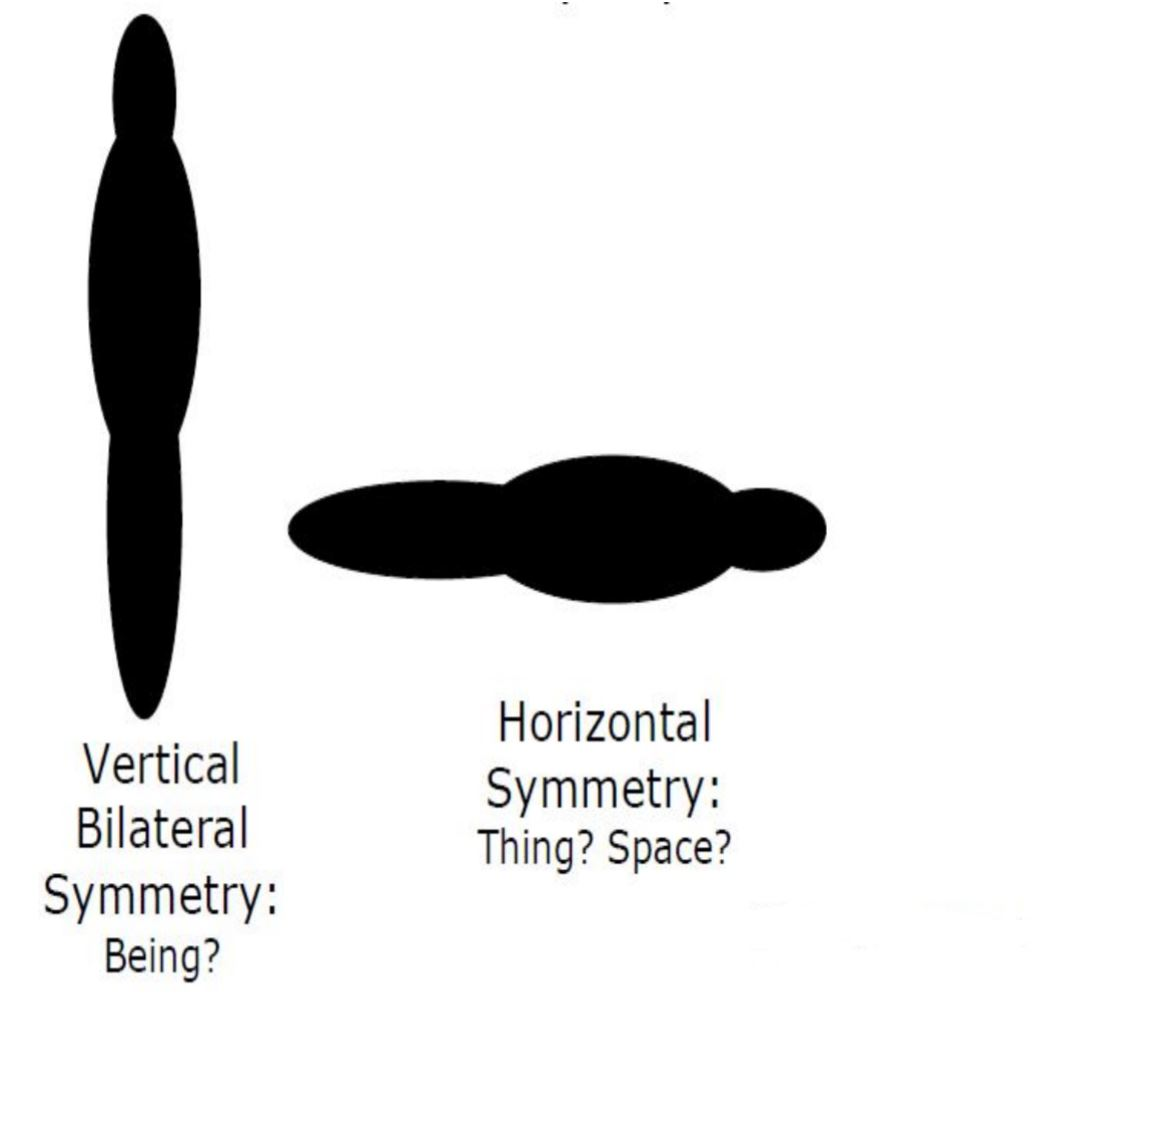
\includegraphics[scale= 0.3]{Abbildungen/Symmetry.JPG}
			\caption[Vertical and horizontal beeings]{\textit{Menschen interpretieren symmetrische Formen um eine vertikale Achse eher als menschlich, als Formen um die horizontale Achse \citep{biocca2002defining}.}}
			\label{vertical_horizontal}
		\end{footnotesize}
	\end{figure}

In \textit{\autoref{vertical_horizontal}} ist zu erkennen, dass eine menschenähnliche, vertikale-bilateral-symmetrische Repräsentation mehr \textit{Co-Präsenz} erweckt als die horizontale-bilateral-symmetrische Repräsentation \citep[S. 546-551]{thornhill1998relative}.
Vertikale-bilaterale Symmetrie wird mit der körperlichen Gesundheit eines Menschen in Verbindung gebracht. Sogar Weibchen verschiedener Spezies neigen dazu, Partner mit einem höheren Grad an bilateraler Symmetrie für die Fortpflanzung auszuwählen \citep[S. 659–669]{rhodes1998facial} \citep{biocca2002defining} \citep[S. 233–242]{grammer1994human}.

\begin{figure}[b!]
		\begin{footnotesize}
		\centering
			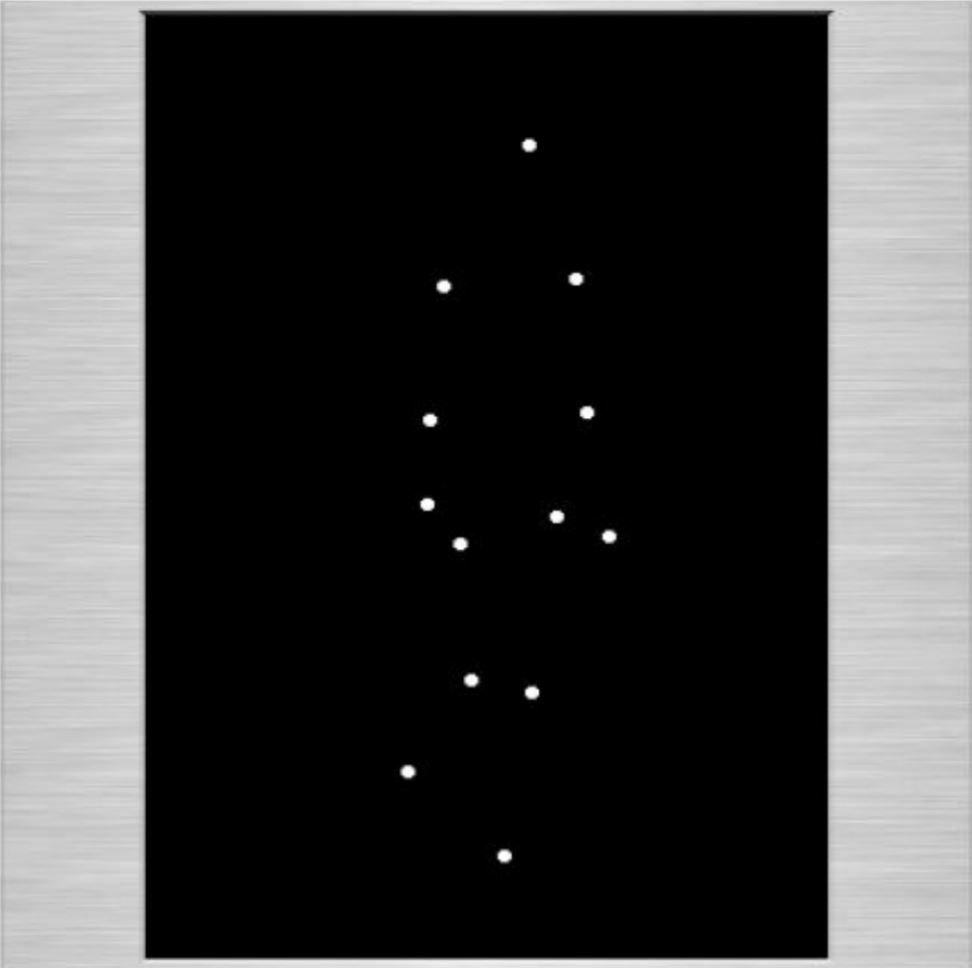
\includegraphics[scale= 0.5]{Abbildungen/moving_dots.JPG}
			\caption[Moving dots]{\textit{Stationäre Punkte, bei denen der Mensch eine lebendige Bewegung ausmachen kann, wenn diese anfangen sich zu bewegen. Es ist sogar möglich einen Menschen zu erkennen sowie dessen Art der Aktivität und seinen emotionalen Zustand \citep{biocca2002defining} \citep[S. 76-89]{johansson1975visual}.}}
			\label{moving_dots}
		\end{footnotesize}
	\end{figure}

Schon sich nur bewegende Punkte können bereits als intelligente Wesen wahrgenommen werden. Johansson \citep[S. 76-89]{johansson1975visual} führte eine Studie durch, in der die Teilnehmer dreizehn sich bewegende Punkte sahen (\textit{\autoref{moving_dots}}) und sofort die Darstellung einer menschlichen Bewegung erkannten. Als die Teilnehmer Punkte sahen, die stationär waren, ist es ihnen nicht möglich gewesen, diese Punkte als menschliche Repräsentation zu erkennen. Wenige sich bewegende Punkte reichen demnach aus, um Informationen zu erzeugen, die Aufschluss über die Aktivität, das Geschlecht, die Bewegung, den emotionalen Zustand oder die Anzahl der Personen geben.

\subsubsection{Vorwärtskinematik vs. inverse Kinematik}
Die Kinematik beschäftigt sich mit der mathematischen Bewegung einzelner Gelenke, ohne dabei die physikalische Kraft zu berücksichtigen \citep[S. 1]{beggs1983kinematics}.

Die \textit{Vorwärtskinematik} beschäftigt sich mit der Frage, wie aus bekannten Positionen und Winkeln einzelner Gelenke, ein Zielpunkt in einem bestimmten Koordinatensystem bestimmt werden kann. Damit ist die \textit{Vorwärtskinematik} das Gegenstück zur \textit{inversen Kinematik} \citep[S. 119]{kucuk2006robot}.
\label{inverseKinematik}
Die \textit{inverse Kinematik} beschäftigt sich damit, herausfinden, wie Gelenke eines Roboterarms bewegt und gedreht werden müssen, um beispielsweise einen Gegenstand von Punkt A nach Punkt B zu bewegen. Es werden anhand der Position des Zielpunkts, alle Winkel der zugehörigen Gelenke approximiert, um somit ihre zugehörigen Rotationen zu bestimmen \citep[S. 299-300]{d2001learning}. Inverse kinematische Berechnungen können auf die Körperteile eines Avatars angewendet werden, um ihn zu animieren. Benutzt eine Person in einem \ac{sve} einen invers kinematisch dargestellten \textit{Selbst-Avatar}, kann sie die Torsorotation, Armbewegungen oder Beinbewegungen seines eigenen Avatars sehen \citep[S. 1]{kim2018real}.

\subsubsection{Einfluss von Avataren}
In der \ac{vr} und in einigen anderen computerbasierten Medien kann sich der Nutzer Avatare erstellen und mit diesen interagieren \citep[S. 1]{neustaedter2009presenting}.

\paragraph{Einfluss des Selbst-Avatars}
\ac{hmd}s beeinflussen das Sichtfeld des Nutzers so stark, dass diese ihren eigenen Körper nicht mehr sehen können. Um diesem Nachteil entgegenzuwirken, kann einem Nutzer ein virtueller Körper zur Verfügung gestellt werden. Dieser Körper wird \textit{Selbst-Avatar} genannt.
Es ist schwierig, einen \textit{Selbst-Avatar} hoher Qualität zu simulieren. Dazu wären das Verfolgen und Animieren mehrerer Körperteile nötig. Ist der \textit{Selbst-Avatar} schlecht animiert oder entstehen während der Nutzung Trackingfehler, die der Nutzer erkennt, kann es sehr leicht zu einem \textit{Break-In-Presence} kommen. Bei diesem \textit{Break-In-Presence} bricht die gesamte Illusion der \ac{vr} für den Nutzer in sich zusammen. 
Dies ist auch der Grund, weshalb relativ wenige \ac{vr}-Anwendungen einen menschlichen Körper als Avatar darstellen.
Sind jedoch genügend Körperteile getrackt und animiert, muss der Avatar nicht unverwechselbar menschlich aussehen, um ein glaubwürdiger \textit{Selbst-Avatar} zu sein. Selbst grobe Avatar-Darstellungen schaffen es, ausreichende Informationen eines menschlichen Körpers zu vermitteln und dadurch glaubwürdig zu wirken \citep{lok2003effects}.

Biocca forschte umfangreich über den Einfluss von \textit{Selbst-Avataren} auf den Nutzer in der \ac{vr} \citep[421-427]{construal2014connected}. Er untersuchte, wie sich die Interaktion mit der Welt verändert, wie sich soziale Interaktionen verändern und wie Aufgaben wahrgenommen und bearbeitet werden \citep{benford1995user} \citep{bowers1996talk}.
Biocca geht in seinen Studien davon aus, dass ein menschenähnlicher Körper als Avatar die \textit{Selbstpräsenz} stark erhöht. Damit die \textit{Selbstpräsenz} weiter erhöht wird, kann ein invers kinematisch simulierter Avatar als \textit{Selbst-Avatar} genutzt werden \citep[421-427]{construal2014connected}.

Dodds et al. fanden heraus, dass ein \textit{Selbst-Avatar} einen wichtigen Faktor zur Erhöhung der Kommunikation in einem \ac{sve} darstellt \citep[1-11]{dodds2011talk}.

Es wurden zahlreiche weitere Studien durchgeführt, um den Einfluss von Avataren zu erforschen. So gibt es Experimente, die den Einfluss des Geschlechts \citep{slater2010first}, der Hautfarbe \citep{peck2013putting} oder des Grades des Realismus \citep{roth2016avatar} untersuchen.

\label{AvatarTrust}
\paragraph{Einfluss der Menschenähnlichkeit des Avatars}
Es stellt sich die Frage, ob ein Avatar in einer \ac{vr} menschenähnlich aussehen sollte. Dieser Frage gingen George et al. \citep{george2018trusting} in ihrer Forschung nach und verglichen, ob sich mehr Vertrauen zwischen einem menschenähnlichen oder einem roboterartigen Avatar aufbauen lässt.
Dazu schufen sie ein Szenario, in dem Personen mittels eines \ac{hmd} ein Social-Dilemma-Scenario\footnote{Situationen, in denen - die rationale Verfolgung von Eigeninteressen zu einer kollektiven Katastrophe führen kann.} erlebten. Sie fanden keinen signifikanten Unterschied in der Vertrauenswürdigkeit zwischen menschenähnlichen und roboterartigen Avataren. Jedoch wurde ein größeres Gefühl von Gemeinsamkeit festgestellt, wenn mit einem menschenähnlichen Avatar interagiert wurde.
% \citep{kerr1983motivation}.
George et al. erwähnten weiterhin in ihrer Studie, dass gute Grafik und realistisches Verhalten durch beispielsweise Mikrogestikulationen und soziale Interaktionen den Aufbau von \textit{Co-Präsenz} unterstützen \citep{george2018trusting}.

Um den Einfluss des Grades an Realismus unter Avataren zu erforschen, führten Riedl et al. \citep{riedl2014trusting} eine Studie zum Vertrauensaufbau unter Menschen im Vergleich zu Avataren mit menschenähnlichen Gesichtern durch. Sie fanden heraus, dass es Personen leichter fällt, einer realen Person, zu vertrauen als einem Avatar mit menschenähnlichem Gesicht. Es wurde der Frontalkortex - die Gehirnregion, die dafür verantwortlich ist, die Gedanken und Gefühle des Gegenübers zu erahnen - bei Interaktionen mit Menschen mehr angeregt als bei Interaktionen mit Avataren mit menschenähnlichen Gesichtern.
Vertrauen zwischen Menschen wird jedoch in der gleichen Geschwindigkeit aufgebaut wie zwischen Menschen und Avataren.

Somit lässt sich feststellen, dass ein höherer Grad an Realismus den Vertrauensaufbau fördert, jedoch kein signifikanter Unterschied in der Geschwindigkeit  des Vertrauensaufbaus zwischen einem menschenähnlichen sowie roboterähnlichen Avatar besteht. Diese Vermutung bestätigten auch Bente et al. \citep[S. 54-59]{bente2004social}, indem sie eine Studie zur \textit{sozialen Präsenz} von Avataren in einem \ac{sve} durchführten. Der Aufbau des \ac{sve} ähnelte einer Videokonferenz. Es waren keine \ac{hmd}s vorhanden und die Teilnehmer haben sich während des Experiments nicht gesehen. In der Studie wurden die Kommunikationsarten, Face-to-Face, Chat und auf Avataren basierende Kommunikationsmedien untereinander verglichen, um Unterschiede in der \textit{Sozialen-Präsenz} sowie dem zwischenmenschlichen Vertrauen zu untersuchen.
Es wurde festgestellt, dass wenig \textit{kognitives Vertrauen} während der Nutzung des \ac{sve} zu Avataren aufgebaut werden konnte, während Face-to-Face, Telefon- und Chatkommunikationen besser abschnitten. Weiterhin wurde weniger \textit{affektives Vertrauen} im \ac{sve} als bei der Nutzung eines Telefons oder während der Face-to-Face Kommunikation aufgebaut.
Bente et al. \citep[S. 54-59]{bente2004social} gehen davon aus, dass dies mit der Neuheit der Technologie zusammenhängt.

\subsubsection{Uncanny-Valley}
\label{Uncanny-Valley-Effekt}
Je menschenähnlicher ein Roboter (u.a. auch ein Avatar) aussieht und je mehr menschenähnliche Bewegungen ein Roboter ausführt, desto mehr positive Gefühle bringt dieser den Personen entgegen, die mit ihm in Berührung kommen. Ab einem bestimmten Punkt des Realismus schlägt dieses Phänomen jedoch um und der Roboter wirkt vielmehr verstörend und ruft  Ablehnung und Angst hervor. Dieses Phänomen und dieser exakte Grad des Realismus wird als Uncanny-Valley Effekt bezeichnet. In \textit{Abbildung \ref{Uncanny-Valley}} ist eine Beschreibung des Effektes zu sehen \citep[S. 352-353]{gast2011unheimliche}.

\begin{figure}[H]
		\begin{footnotesize}
		\begin{center}
			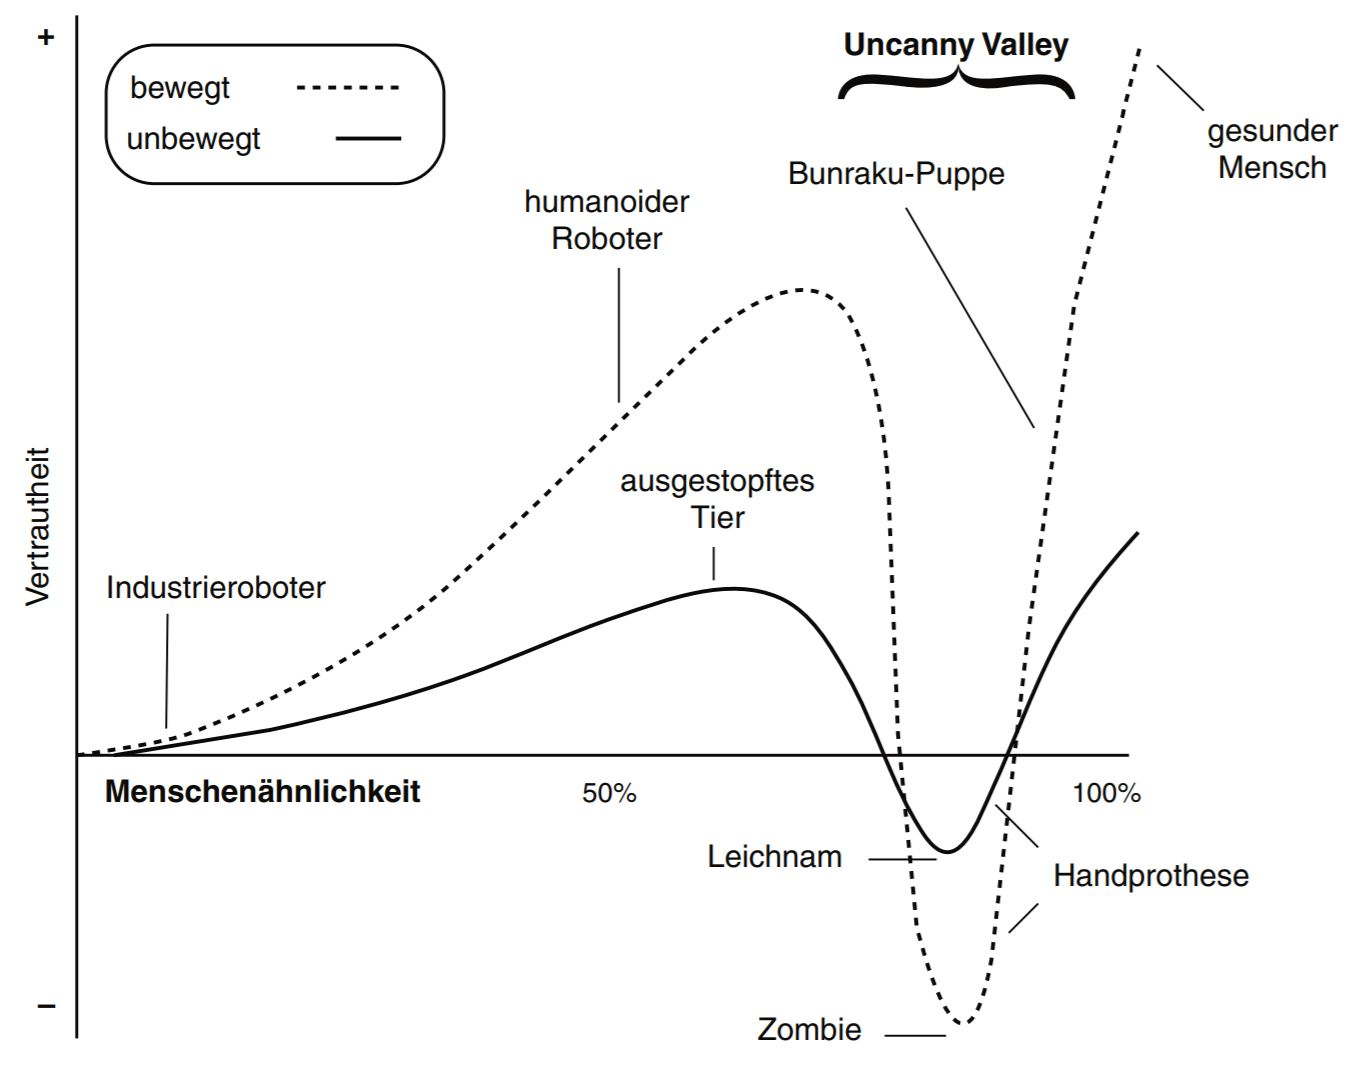
\includegraphics[scale=.45]{Abbildungen/Uncanny-Valley.JPG}	
			\caption[Der Uncanny-Valley Effekt]{Der Uncanny-Valley Effekt beschreibt das Gefühl des Unbehagens ab einem gewissen Realitätsgrad.}
			\label{Uncanny-Valley}
		\end{center}
		\end{footnotesize}
	\end{figure}	
%Connected to My Avatar:
%Effects of Avatar Embodiments on User Cognitions, Behaviors,
%and Self Construal 
%
%421
%https://sci-hub.do/10.1007/978-3-319-07632-4 
%file:///B:/Chrome%20Downloads/Biocca2014_Chapter_ConnectedToMyAvatar.pdf 
%Emotional Contagion with Artificial Others. Effects
%of Culture, Physical Appearance, and Nonverbal Behavior
%on the Perception of Positive/Negative Affect in Avatars 	
%412
%https://sci-hub.do/10.1007/978-3-319-07632-4
%https://dl.acm.org/doi/fullHtml/10.1145/223904.223935?casa_token=B8tEKM39OVQAAAAA:VNilOxaXG3_2Bw-bEClS10xyOXLBxB8ymyo4B-d1kUoAmCgWC1MDdVKSptRADsBaGw19nzE15dwIWQ
%http://mcneilllab.uchicago.edu/pdfs/dmcn_vietri_sul_mare.pdf
%https://sci-hub.ren/https://doi.org/10.1371/journal.pone.0025759 SEITE 2
\newpage

	\subsection{Teams}		
	\label{Teamwork}
%Was ist ein Team? Wie unterscheidet sich ein "normales" Team von einem Team, welches räumlich voneinander getrennt ist? "Normale" Teams, haben die Möglichkeit sich jederzeit oder mit einem geringem Zeitaufwand von Angesicht zu Angesicht zu treffen, während räumlich voneinander getrennte Teams nicht diese Möglichkeit besitzen.
%Im folgenden Kapitel wird definiert, was unter einem Team, einem Virtuellen Team, Teambuilding und Teamtraining verstanden wird.
\label{team}
	Ein Team wird als eine \glqq{} kleine Anzahl von Personen mit sich ergänzenden Fähigkeiten, die sich gleichermaßen einem gemeinsamen Zweck, Ziel und Arbeitsansatz verpflichtet fühlen\dq{} \citep[S. 2]{zenun2007effects}, definiert.
	
Das Verhalten von Personen, die in einem Team arbeiten, lässt sich in \textit{Teamwork} und in  \textit{Taskwork} unterteilen \citep[S. 541-542]{rousseau2006teamwork}.
 \textit{Taskwork} beschreibt dabei, wie die Ausführung von Kernkompetenzen in einem bestimmten Bereich aussieht sowie welche Aufgabe ein Team ausführt.
 \textit{Teamwork} beschreibt die gemeinsame Arbeitsleistung \citep[S. 357]{marks2001temporally}.
 
Die wirtschaftliche Leistung von Unternehmen hängt häufig stark von der Arbeitseffizienz gut funktionierender Teams ab. Gut funktionierende Teams können dabei helfen, die wirtschaftliche Leistung zu verbessern, indem Mitglieder eines Teams weniger Fehler durch bessere Entscheidungen erzeugen \citep[S. 1-6]{biech2007pfeiffer}. 
%Cohen und Bailey \citep[S. 557]{cohen1997makes} definieren ein Team als \glqq{}eine Ansammlung von Individuen, die in ihren Aufgaben voneinander abhängig sind, die die Verantwortung für die Ergebnisse teilen, die von sich selbst und von anderen als eine intakte soziale Einheit gesehen werden."
%
%Sala \citep[S. 541]{salas2008teams} definiert ein Team als "die voneinander abhängigen Leistungskomponenten, die erforderlich sind, um die Leistung mehrerer Personen effektiv zu koordinieren".
%\textbf{Teambuilding} zielt dabei darauf ab, die Haltung oder Einstellung der Personen innerhalb und untereinander eines Teams zu verbessern um das gesamte Team zu verbessern, während \textbf{Teamtraining} drauf abzielt, spezielle Fähigkeiten einzelner Personen zu fördern um das gesamte Team punktuell zu stärken \citep[S. 367-369]{shuffler2011there}.
\subsubsection{Virtuelle Teams}
\label{vts}
%https://sci-hub.ren/10.1111/j.1365-2575.2009.00326.x
\textit{Virtuelle Teams} teilen viele Eigenschaften herkömmlicher \textit{Teams}. Es muss jedoch unterschieden werden, wie die virtuelle Komponente des Teams definiert wird und weshalb diese Komponente ein herkömmliches Team zu einem virtuellen Team macht \citep[S. 270]{schweitzer2010conceptualizing}.

Laut Ebrahim et al. \citep{ale2009virtual} können virtuelle Teams in vier Kategorien unterteilt werden.
Diese sind \textit{Telearbeit}, \textit{virtuelle Gruppen}, \textit{virtuelle Teams} und \textit{virtuelle Gemeinschaften}.
\textit{Telearbeit} liegt vor, wenn eine Person von außerhalb des Hauptarbeitsplatzes arbeitet. \textit{Virtuelle Gruppen} sind mehrere \textit{Telearbeiter} unter einem Vorgesetzten zusammengefasst.
\textit{Virtuelle Gemeinschaften} sind Gemeinschaften, die nicht unter einer Organisationsstruktur arbeiten und von gemeinsamen Zielen, Rollen und Normen geleitet werden. Ein Beispiel dafür ist die gemeinschaftliche Bearbeitung eines Open-Source-Softwareprojekts. Ein \textit{virtuelles Team} liegt vor, wenn mehre Mitglieder einer virtuellen Gruppe miteinander arbeiten und dasselbe Ziel verfolgen.
 
\textit{Virtuelle Teams} besitzen laut Schweizer et al. \citep[S. 270]{schweitzer2010conceptualizing}\footnote{Die vollständige Liste von Schweizer et al. befindet sich in \textit{\autoref{criteriaForVirtualTeams}}.} noch vier weitere Kennzeichen, um als \textit{virtuelles Team} zu gelten. Laut ihnen sind diese:
\label{AnforderungenLautSchweitzer}
\begin{itemize}
\item Zustande gekommen mithilfe von Kommunikationstechnologie. Durch technische Hilfsmittel wird kommuniziert, es werden Entscheidungen getroffen oder Informationen ausgetauscht.
\item Räumlich getrennt. \textit{Virtuelle Teams} arbeiten \textit{nicht} am selben Arbeitsplatz.
\item Grenzübergreifend. Die Teammitglieder stammen aus verschiedenen Organisationen oder Organisationseinheiten.
\item Asynchron. \textit{Virtuelle Teams} arbeiten zu unterschiedlichen Zeiten, in verschiedenen Zeitzonen oder in derselben Zeitzone in unterschiedlichen Schichten.
\end{itemize}

Einige Autoren nehmen in ihre Definition eines \textit{virtuellen Teams} den Aspekt der zeitlichen Limitierung oder der kulturellen Diversität auf. So besteht ein \textit{virtuelles Team} für Jarvenpaa et al. \citep[S. 1-2]{jarvenpaa1999communication} nur für einen bestimmten Zeitraum und es ist zusätzlich kulturell divers.

Infolge der immer stärker werdenden globalen Vernetzung kann fast jedes Team als eine Art \textit{virtuelles Team} bezeichnet werden, denn nur selten arbeiten Teams heutzutage ohne Kommunikationstechnologie. 
Es wird davon ausgegangen, dass Virtualität als Kontinuum gesehen werden kann, bei dem jedes Team ein gewisses Maß an Virtualität besitzt. Dieses Kontinuum reicht von Face-to-Face bis zur vollständigen, nur über Kommunikationstechnologie stattfindenden Kommunikation \citep{martins2004virtual} (siehe \textit{Abbildung \ref{virtualTeamsVirtuality}}).

\begin{figure}[H]
		\begin{footnotesize}
		\centering
			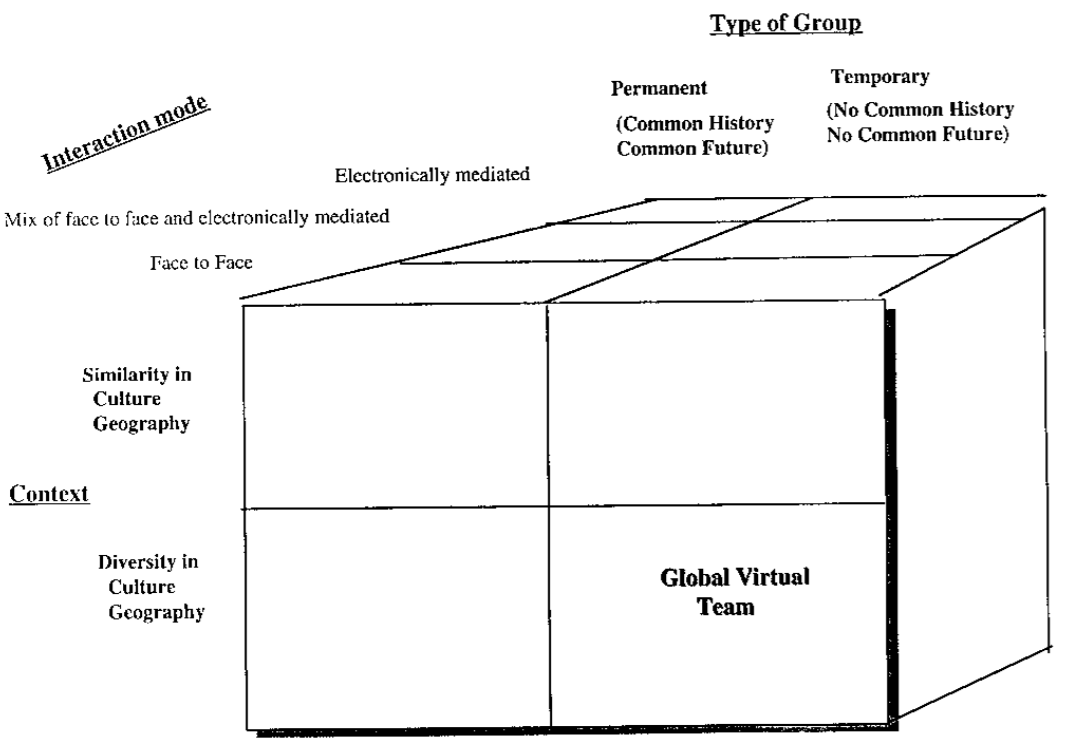
\includegraphics[scale=0.6]{Abbildungen/GlobalVirtualTeam.PNG}	
			\caption[Virtualität eines virtuellen Teams]{Grad an Virtualität, das ein Team laut Javenpaa et al. \citep{jarvenpaa1999communication} besitzen muss, um als \textit{virtuelles Team} zu gelten.}
			\label{virtualTeamsVirtuality}
		\end{footnotesize}
	\end{figure}
%Aus heutiger Sicht, muss ein virtuelles Team nicht zwangsläufig aus verschiedenen Organisationen bestehen oder asynchron arbeiten. In vielen Unternehmen ist es auch möglich, dass ein virtuelles Team in derselben Zeitzone und ohne kulturelle Diversität oder zeitliche Limitierung zusammenarbeitet.
%Somit bleiben nur noch die Komponenten des Zusammenfindens mithilfe von Kommunikationstechnologie sowie der räumlichen Trennung.
%
%Wird nun die Definition eines Teams von Zenun et al. \citep[S. 2]{zenun2007effects} herangezogen, und die virtuelle Komponente in diese mit eingebracht, kann ein virtuelles Team als
%\begin{quote}
%\glqq{}eine kleine, auf Kommunikationstechnologie basierende, räumlich getrennte Gruppe, von Menschen mit gleichartigen Fähigkeiten, welche sich in gleicher Weise für das gleiche Ziel und gleiche Arbeitsweisen einsetzen und dies verfolgen\dq{} \\
%definiert werden.
%\end{quote}


\subsubsection{Aufbau eines virtuellen Teams}
\label{Aufbau eines virtuellen Teams}
%	https://sci-hub.tw/https://doi.org/10.1108/13527590110395621
%Seit einigen Jahren wird die Wichtigkeit von effektiven Teambuildingmaßnahmen in der strategischen Organisationsentwicklung erkannt. Dabei spielt der Wandel hin zu einer globalen, auf Wissen basierten Wirtschaft eine zentrale Rolle \citep{belbin2011management} \citep[S. 7]{katzenbach2015wisdom}.
%Wirtschaftlicher Erfolg korreliert direkt mit der Fähigkeit eines Unternehmens, Teams organisieren, strukturieren und managen zu können \citep{pasmore1993designing}.
%Der Erfolg eines \textit{virtuellen Teams} ist somit als Nebenprodukt der organisatorischen Fähigkeiten eines Unternehmens zu verstehen \citep[S. 5]{kling1994social}.
%
%Erfolgreiches Teambuilding kann die \textit{Effektivität} eines \textit{virtuellen Teams} steigern und dazu führen, dass Personen sich mehr mit dem Team identifizieren \citep{kaiser2000student}.
\textit{Virtuelle Teams} werden häufig aufgrund eines anstehenden Projektes gebildet und wieder aufgelöst, wenn das Projekt beendet ist. Somit sind \textit{virtuelle Teams} oftmals nur von kurzer Lebensdauer. Dies impliziert auch, dass die Aufgabenverteilung in virtuellen Teams je nach Projekt oder Aufgabe immer unterschiedlich ist und keine einheitliche Hierarchie innerhalb des \textit{virtuellen Teams} zustande kommt \citep{wong2000virtual}.

Auch um räumliche oder kurzzeitige Trennungen eines Teams zu umgehen, werden \textit{virtuelle Teams} gegründet. Dabei werden computergestützte Technologien so verwendet, dass räumlich getrennte Teammitglieder ihre Aufgaben mittels computergestützter Kommunikation im Team koordinieren können \citep[S.  117-119]{peters2007identifying} \citep[S. 1-2]{cascio2003leadership}.
Das \textit{virtuelle Team} zu gründen, stellt laut Dyer nicht die eigentliche Herausforderung dar. Die Herausforderung ergibt sich aus den unterschiedlichen Kulturen, Entfernungen und Zeitzonen, die ein \textit{virtuelles Team} mitbringt. Wenn die einzelnen Teammitglieder eines \textit{virtuellen Teams} sich gegenseitig vertrauen, kann der eigentliche Nachteil der verschiedenen Kulturen, Entfernungen und der Zeitzonen auch zum Vorteil werden. Es wird kulturelle Diversität gefordert und neue Verhaltensmuster erworben, wodurch neue, kreative Sichtweisen gefördert werden. Durch diese Faktoren ist es möglich, innovativer zu arbeiten und zu denken \citep{dyer1995team} \citep[S. 405-416]{milliken1996searching}.

Gerade für \textit{virtuelle Teams} ist die Anfangsphase der Teamgründung von entscheidender Bedeutung. 
Die Art und Weise \textit{wie} kommuniziert wird, ist in dieser Phase sehr ergebnisorientiert. Defizite in der Kommunikation kann die Schlüsselfaktoren (soziale und emotionale Beziehungsbildung sowie den Aufbau von Vertrauen) eines erfolgreichen Teams beeinträchtigen \citep[S. 378]{ren2007applying}.
Die Mitglieder eines \textit{virtuellen Teams} haben im Gegensatz zu traditionell geformten Teams weniger Möglichkeiten, sich zu sehen, zu interagieren oder Konflikte zu lösen. 
Respekt und gegenseitiges Verständnis sind die Grundbausteine, um Kreativität und Innovation innerhalb eines Teams zu fördern. Die Effektivität eines Teams ist eine direkte Konsequenz daraus \citep[S. 378]{ren2007applying}.

Eine ideale Teamgründung in einem \textit{virtuellen Team} ist aufgrund der räumlichen Trennung nicht möglich. 
Für eine optimale Situation sollte in einem schon bestehenden Team eine virtuelle Komponente hinzugefügt werden, um auf die Vorteile von schon vorhandenen sozialen Bindungen zugreifen zu können. Folglich sollte sichergestellt werden, dass \textit{virtuelle Teams} während ihres Bestehens bestmöglich in ihrem Aufbau von Vertrauen und sozialen Beziehungen unterstützt werden, um eine maximale \textit{Teameffektivität} zu erreichen \citep[S. 36-37]{holton2001building}.

\subsubsection{Teameffektivität}
\label{Teameffektivität}
\textit{Teameffektivität} ist die Fähigkeit eines Teams, so miteinander zu interagieren und sich so zu unterstützen, dass ein zuvor definiertes Ziel des Teams erreicht wird. Da viele externe Faktoren zum Erreichen des Ziels beitragen können, ist es wichtig, dass das Team immer einen Fokus auf seine \textit{Teameffektivität} hat \citep[S. 557]{salas2005there}.

Es gibt keinen einheitlichen Standard, um die Effektivität eines Teams zu messen. Es wird davon ausgegangen, dass die Effektivität in Gruppen anhand der von der Gruppe produzierten Ergebnissen (Quantität, Qualität, Geschwindigkeit, Kundenzufriedenheit) gemessen werden kann. Der Effekt, dass eine Gruppe Einfluss auf die Produktivität der einzelnen Mitglieder hat, trägt dabei zur Verbesserung der Gesamteffektivität bei \citep[S. 309]{guzzo1996teams}.

Lin et al. \citep{lin2008model} gehen davon aus, dass \textit{Teameffektivität} anhand der Zufriedenheit mit den erzielten Teamergebnissen, der Zufriedenheit mit dem Arbeitsprozess des Teams sowie dem Ausmaß der erzielten Teamleistung bestimmt werden kann.
Jedoch wird die \textit{Teameffektivität} auch von subjektiven Eigenschaften wie der Diversität des Teams, dem Teamzusammenhalt oder der Kommunikation innerhalb des Teams beeinflusst. 

\paragraph{Teameffektivität in virtuellen Teams}
\label{TEinVT}
\textit{Virtuelle Teams} leisten, in Verbindung mit diesen subjektiven Eigenschaften und aufgrund ihrer Anpassungsfähigkeit, durch flache hierarchische Prozesse und erhöhter Kreativität durch Diversität, einen wesentlichen Beitrag zur \textit{Teameffektivität} \citep{handke2019alles} \citep{becker2002fuhrung}.

Wird ein Vergleich zwischen \textit{traditionell} geformten Teams und \textit{virtuellen Teams} gezogen, gehen Schweitzer et al. \citep{schweitzer2010conceptualizing} davon aus, dass traditionell geformte Teams effektiver als \textit{virtuelle Teams} sind und die \textit{Teameffektivität} abnimmt je höher der Grad an Virtualität (siehe \textit{Abbildung \ref{virtualTeamsVirtuality}}) ist.
Diese Meinung teilen auch Becker et al.. Laut ihnen leidet der Austausch des Informationsgehaltes sowie der Vertrauensbildung aufgrund steigender Virtualität und es kann nicht dieselbe Effektivität wie in einem Face-to-Face Team erreicht werden \citep{becker2002fuhrung}.
Eine andere Meinung nehmen dabei Dufner et al. ein \citep{dufner2002asynchronous}. Ein zeitlich asynchroner Informationsaustausch von \textit{virtuellen Teams} hat laut ihrer Untersuchung einen positiven Einfluss auf die \textit{Teameffektivität}, da die Teammitglieder mehr Zeit haben, um über Probleme nachzudenken, bevor Informationen ausgetauscht werden.

Bisherige Studien haben positive Zusammenhänge \citep{davis2000trusted}, keine Zusammenhänge \citep{hertel2004managing} sowie negative Zusammenhänge \citep{dirks1999effects} zwischen Vertrauen und \textit{Teameffektivität} in \textit{virtuellen Teams} festgestellt.
Trotz der sich widersprechenden Studienergebnisse wird im Allgemeinen die Meinung vertreten, dass Vertrauen einen positiven Einfluss auf die \textit{Teameffektivität} besitzt \citep{de2016trust}. 
Vertrauen in sein Team hilft dabei, eigene Unsicherheiten auszublenden, um sicherer und effektiver arbeiten zu können \citep{de2010does}. Weiterhin entsteht durch vorhandenes Vertrauen in sein Team ein größeres Interesse an den Teammitgliedern, was Synergieeffekte freischaltet und eine direktere und effektivere Interaktion ermöglicht \citep{dirks1999effects}. 
%Es wird angenommen, dass starkes \textit{zwischenmenschliches Vertrauen} die Teameffektivität positiv beeinflusst \citep{mcallister1995affect} \citep{mayer1995integrative} \citep{dirks2002trust}.
	
%Das Trainieren eines Teams kann ihre gesamte Effektivität steigern. Dies scheint am effektivsten, wenn mehrere Charakteristika des Teamworks auf einmal angesprochen werden. Diese sollten auch experimentelle Aktivitäten beinhalten, um aktiv lernen und üben zu können \citep[19]{mcewan2017effectiveness}.

%Gemeinsames Training führt zu einer Steigerung der Qualität der Ideen und Entscheidungen sowie der gesamten Teamleistung.
%Die Kommunikation untereinander wird gefördert, da die einzelnen Teammitglieder gegenseitig ihre Aufgaben kennen und dadurch eher bereit sind sich untereinander zu helfen.
%Training im Team geht mit einem besseren Verständnis über das Wissen der anderen Teammitglieder einher, denn somit können auch individuelle Stärken gefördert und Schwächen durch andere Teammitglieder kompensiert werden.
%Ein solches Team bringt ein Gefühl von Sicherheit mit sich, was zu einer erhöhten Risikobereitschaft führt. Dies kann die Kreativität der eingebrachten Ideen stärken und Teammitglieder können an der Möglichkeit, größere Risiken einzugehen, wachsen \citep[S. 2-4]{biech2007pfeiffer}.
%Dies führt zu einer Steigerung der Qualität der Ideen und Entscheidungen sowie der gesamten Teamleistung.
%Auch das soziale Identitätsgefühl hängt davon ab, ob ein generelles Gruppenverständnis besteht, eine Person sich der Gruppe zugehörig fühlt und ob man sich als Gruppe mit anderen Gruppen vergleicht. Gruppenzugehörigkeit ist ein wichtiger Bestandteil des Selbstverständnisses eines Individuums \citep{sutantovicious}.
%	
%Ist ein Gefühl von Gruppenzugehörigkeit gegeben, stärkt dies die Gruppenproduktivität sowie die individuelle Leistungsfähigkeit. Weiterhin führt es zu einem besseren Zusammenhalt, mehr Vertrauen \citep{herbsleb2000distance}, besserer Kommunikation und Kooperation untereinander \citep[S. 510]{olson2003psychological}.

\newpage

\subsection{Vertrauen}
\label{Vertrauen}
Der Begriff \textbf{Vertrauen} beschreibt ein psychologisches Konzept, das jeden Menschen ständig begleitet.
Ein Politiker wirbt um das Vertrauen seiner Wähler, Unternehmer beschreiben sich selbst als \glqq{}Geschäftspartner des Vertrauens\grqq{} oder es wird der \glqq{}Arzt des Vertrauens\dq{} empfohlen.

Vertrauen im Zusammenhang mit dem Begriff \textit{\ac{vr}} kann auf zwei unterschiedliche Arten und Weisen betrachtet werden. 
%	https://sci-hub.tw/https://doi.org/10.1177/1046496408323569
Während Vertrauen in die \ac{vr}-Technologie sich mit der Akzeptanz der Technologie an sich beschäftigt, beschäftigt sich \textit{zwischenmenschliches Vertrauen} mit dem Vertrauen zwischen zwei oder mehreren Personen \citep{mcknight2011trust}.
%\citep[S. 10]{trustInVRTechnology}
%Mangelndes Vertrauen in eine Technologie, kann Nutzer dran hindern, diese zu Nutzen. \citep{trustInVRTechnology}

Da sich diese Arbeit mit dem zwischenmenschlichen Vertrauen beschäftigt, wird das Vertrauen in die Akzeptanz der \ac{vr} nicht weiter behandelt.
%Vertrauen wird in dieser Ausarbeitung als bilaterales Konstrukt zwischen einer vertrauenden Person und einer zu vertrauenden Person definiert.
% https://sci-hub.ren/10.4337/9781847202819.00008
% https://sci-hub.ren/10.4337/9781847202819.00008
\subsubsection{Das Konstrukt Vertrauen}
\label{Konstrukt des Vertrauens}
Aufgrund der Vielseitigkeit von Vertrauen, gibt es unterschiedliche Definitionen. \newline
Eine der ersten Definitionen von Vertrauen wurde 1967 von Rotter aufgestellt. Er definiert Vertrauen als 
\begin{quote}
\glqq{}die Erwartung eines Individuums oder einer Gruppe, dass man sich auf das Wort, das Versprechen, die mündliche oder schriftliche Aussage eines anderen Individuums oder einer Gruppe verlassen kann\dq{} \citep[S. 651]{rotter1967new}.
\end{quote}
Die jedoch meist verbreitete Definition stammt von Meyer et al. \citep[S. 712]{mayer1995integrative}. So definieren sie Vertrauen als:
\begin{quote} \glqq{}die Bereitschaft einer Person, für die Handlungen einer anderen Person anfällig zu sein, basierend auf der Erwartung, dass der Vertrauensnehmer eine bestimmte, für den Vertrauensgeber wichtige Handlung ausführen wird, unabhängig von der Möglichkeit, diese Person zu überwachen oder zu kontrollieren.\dq{} \end{quote}
Jede zwischenmenschliche Beziehung beginnt mit einer frühen Phase der Vertrauensbildung. Diese frühe Phase kann von Unsicherheiten und Zweifel geprägt sein. Das gegenseitige Vertrauen, das man sich anschließend schenkt, muss anfänglich erst einmal ausgelotet werden \citep[S. 166-168]{meyerson1996swift}.
Während der frühen Phase der Vertrauensbildung entscheidet sich, ob eine Beziehung aufrechterhalten wird oder nicht. Unterbewusst bildet sich ein Gefühl von Zuversicht und Sicherheit oder ein Gefühl von Spannung, Zweifel und Skepsis dem Interaktionspartner gegenüber. 
Dabei ist es egal, ob sich dafür entschieden wird, jemandem zu vertrauen, oder nicht. Auf jeden Fall beeinflusst die Stärke des positiven oder negativen Vertrauensgefühls die Effektivität der Zusammenarbeit. Vertrauen kann es einfach oder schwierig machen, mit einer anderen Person zu arbeiten und Ziele in einer Gruppe oder einem Team zu erreichen.
Früher Vertrauensaufbau ist daher der Schlüssel zur erfolgreichen Zusammenarbeit \citep[S. 405-406]{bigley1998straining}.
Die initiale Phase der Vertrauensbildung wirkt sich auf das \textit{kognitive} und das \textit{affektive Vertrauen} aus, welche einen starken Einfluss auf das sich entwickelnde Vertrauensmodell zu einer Person haben. In dieser Phase sind diese beiden Vertrauensarten anfällig für Veränderungen \citep[S. 461-462]{baldwin1992relational}.
Meinungen und Annahmen, die sich frühzeitig bilden, prägen somit stark die zukünftige Meinung über die vertrauensnehmenden Personen.

Auch im Unternehmertum muss sich mit dem Konzept des Vertrauens beschäftigt werden, um erfolgreich arbeiten zu können. Ohne Vertrauen in ein Team oder in unterschiedliche Personen, fällt es schwer, Risiken einzugehen. Ist Vertrauen vorhanden, wird man nicht mit der Angst konfrontiert, dass andere Personen einen ausnutzen könnten. Betrachtet man Vertrauen im Unternehmen auf der Ebene von Teams, setzen sich die vertrauensgebenden Personen sowie die vertrauensnehmenden Personen aus mehreren Teammitgliedern zusammen \citep[S. 1152]{breuer2016does}.

Vertrauen wird nicht statisch und einseitig betrachtet. Eine Person kann nicht nur \textit{vertrauen} oder \textit{nicht vertrauen}. Vertrauen ist ein dynamisches Konstrukt, welches sich mit der Zeit verändert. Es kann in eine Bildungs-, Stabilisierungs- und Abnehmphase unterteilt werden \citep[S. 396]{rousseau1998not}.

Viele Psychologen, die sich mit dem Thema Vertrauen beschäftigen, gehen heute davon aus, dass \textit{zwischenmenschliches} Vertrauen aus einem zweidimensionalen Konstrukt besteht \citep{johnson2005cognitive}; \citep{cook1980new}. So sind Mooradian et al. der Ansicht, dass Vertrauen als \textit{Eigenschaft} oder als \textit{Zustand} gesehen wird \citep[S. 524-525]{mooradian2006trusts}.

\subsubsection{Vertrauen als Eigenschaft }
\label{Vertrauen als Eigenschaft}
Wird Vertrauen als Eigenschaft betrachtet, spiegelt dies die Einstellung zum Vertrauen einer Person wider. Diese Einstellung zum Vertrauen ist langlebig und wird nicht allzu schnell auf oder abgebaut. Unabhängig von einer Situation, in der sich diese Person befindet, wird davon ausgegangen, dass diese Eigenschaft aus dem Temperament oder der Lebenserfahrung einer Person entsteht. Dieses Vertrauen ist das Grundlevel an Vertrauen, das eine Person in eine neue zwischenmenschliche Beziehung von Anfang an mitbringt \citep[S. 11]{couch1996assessment}. Es ist jedoch nicht nachgewiesen, wie \textit{generelles Vertrauen} genau gebildet wird \citep[S. 409]{stolle2002trusting}.

\textit{Generelles Vertrauen} impliziert, dass den meisten Personen vertraut werden kann, oder dass im Fall von generellem Misstrauen, Personen nicht vertraut werden kann \citep[S. 409]{stolle2002trusting}.

\textit{Generelles Vertrauen} ist nicht situationsabhängig, sondern stellt eine längerfristige Konstante auf Basis des Grundvertrauens einer Person dar. Es setzt sich dabei aus der individuellen Eigenschaft des Hangs zum Vertrauen einer einzelnen Person sowie der Grundstimmung gegenüber Personen im Allgemeinen, zusammen \citep[S. 11]{couch1996assessment}.

\subsubsection{Vertrauen als Zustand}
\label{Vertrauen als Zustand-Label}
Wird \textit{Vertrauen als Zustand} betrachtet, so kann sich dieses Vertrauen im Laufe der Zeit, z.B. durch Interaktion mit einer anderen Person, ändern. Dieser Zustand des Vertrauens spiegelt sich auch in der Definition von Mayer et al. von Vertrauen wider \citep[S. 712]{mayer1995integrative}:
\begin{quote}
\glqq{}die Bereitschaft einer Person, für die Handlungen einer anderen Person anfällig zu sein, basierend auf der Erwartung, dass die vertrauensnehmende Person eine bestimmte, für den Vertrauensgeber wichtige Handlung ausführen wird, unabhängig von der Möglichkeit, diese Person zu überwachen oder zu kontrollieren.\dq{}
\end{quote}
Es wird einer Person oder einem Team ein Vertrauensvorschuss gewährt, der sich jedoch jederzeit verändern kann, wenn dieser gebrochen wird.

Das Konzept des \textit{Vertrauens als Zustand} lässt sich laut Lewis et al. \citep[S. 970-971]{lewis1985trust} in zwei Teile unterteilen.
Laut ihren Studien basiert Vertrauen 

\begin{quote}
\glqq{}auf einem kognitiven Prozess, der zwischen vertrauenswürdigen, misstrauischen und unbekannten Personen und Institutionen unterscheidet. In diesem Sinne wählen wir kognitiv aus, wem wir in welcher Hinsicht und unter welchen Umständen vertrauen, und wir stützen die Wahl auf das, was wir als \glqq{}gute Gründe\grqq{} ansehen, die einen Beweis für die Vertrauenswürdigkeit darstellen\grqq{} \citep[S. 970]{lewis1985trust}.
\end{quote}

Somit basiert das \textbf{kognitiv aufgebaute Vertrauen} auf einer von uns definierten Logik statt auf einer emotionalen Komponente. Diese \glqq{}guten Gründe\dq{} können auch leicht gebrochen werden, indem der Vertrauensvorschuss, den wir durch das kognitive Vertrauen unserem Interaktionspartner geben, gebrochen wird.
Das kognitive Vertrauen kann kurzfristig aufgebaut werden und ist leicht anfällig gegen äußerliche Einflüsse \citep[S. 970]{lewis1985trust}. 

Weiterhin besitzt Vertrauen als \textit{Zustand} eine affektive Komponente:
\begin{quote}
\glqq{}Diese \textbf{affektive Komponente des Vertrauens} besteht in einer emotionalen Bindung zwischen allen, die an der Beziehung beteiligt sind. Wie die affektiven Bindungen der Freundschaft und der Liebe schafft Vertrauen eine soziale Situation, in der intensive emotionale Investitionen getätigt werden können, und deshalb weckt der Verrat eines persönlichen Vertrauens ein Gefühl der emotionalen Empörung bei dem Betrogenen. Der Vertrauensbruch trifft die Grundlage der Beziehung selbst, nicht nur den spezifischen Inhalt des Verrats. Diese emotionale Komponente ist bei allen Arten von Vertrauen vorhanden, aber normalerweise ist sie bei engem zwischenmenschlichem Vertrauen am intensivsten\dq{} \citep[S. 971]{lewis1985trust}.
\end{quote}
Ein Beispiel für affektives Vertrauen ist die Liebesbeziehung zwischen zwei Personen. Das affektive Vertrauen baut sich mit der Zeit langsam auf und kann durch verschiedene Ereignisse erschüttert oder gestärkt werden. Es kann eher durch Emotionen statt durch Logik charakterisiert werden.
\textbf{Affektives Vertrauen} ergibt sich aus \textit{zwischenmenschlichen emotionalen Verbindungen und gegenseitiger Fürsorge}, während individuelles \textbf{kognitives Vertrauen} auf der \textit{Überzeugung in die Fähigkeiten oder in die Zuverlässigkeit eines anderen basiert} \citep[S. 30]{mcallister1995affect}.

Vertrauensaufbau zwischen verschiedenen Personen beinhaltet somit zwei Komponenten. Beide Komponenten sind bei der Teamgründung von großer Bedeutung. 
McAllister schreibt diesbezüglich, dass die Grunderwartung der kognitiven Komponente erst einmal erfüllt werden müsse bevor mehr in die Beziehung zu den einzelnen Personen eines Teams investiert werden würde. Je mehr ein Team zusammenarbeitet und sich kennenlernt, umso wichtiger wird die affektive Komponente der Vertrauensbildung \citep[S. 30]{mcallister1995affect}.

Laut Studien von McKnight et al. kann ein starkes Vertrauen in frühen Teamgründungsphasen entstehen. Empfinden Teammitglieder beispielsweise den Teamgründungsprozess als strukturiert, ergibt sich dadurch ein höheres \textit{kognitives Vertrauen} und es folgt ein höheres Gesamtvertrauen in das Team \citep[S. 478-479]{mcknight1998initial}.
%Ich glaube, ich habe die Aufgaben des Versuchsleiters gut erledigt -> Auf Kognitives Vertrauen analisieren Pro person! Hier ist einseitige Signifikanz in der Korrelation von Wie Erfolgreich haben Sie ihrer Meinung nach die vom Versuchleiter ... mit Cog_Trust_Windsorizing vorhanden!
%Weiterhin ist durch eine erhöhte Self-Presence eine bessere Identifizierung seiner Selbst und dem Avatar möglich. 
%Hat nun ein Head und Hand getrackter Avatar einen Einfluss auf die wahrgenommen Fähigkeiten oder die wahrgenommene Zuverlässigkeit in das Team? Genau diese Frage stellt sich diese Hypothese 2.
%Es wird davon ausgegangen, dass, egal welche Kondition des Avatars ein Probant zur Verfügung gestellt bekommt, dies keinen Einfluss auf die wahrgenommenen Fähigkeiten des Teams besitzt. Somit erscheint ein Team in seiner Leistungsfähigkeit und Zuverlässigkeit immer gleich, egal ob ein Avatar menschenähnlich ist oder nicht.
%\textbf{ES GIBT NOCH MEHR VERGLEICHE, SIEHE DAZU QUELLE UNTEN}
%\textbf{HIER EINEN VERGLEICH ZWISCHEN COGNITIVE TRUST UND AFFECTIVE TRUST AUFSTELLEN. AUCH BEIM FRAGEBOGEN BEACHTEN! ERKLÄRUNG GEBEN WARUM GENAU DEN VON MC ALLISTER 1995 GENOMMEN WURDE.}
%\textbf{http://citeseerx.ist.psu.edu/viewdoc/download?doi=10.1.1.496.9380&rep=rep1&type=pdf}
\subsubsection{Vertrauensaufbau in virtuellen Teams}
\label{Vertrauen und virtuelle Teams}
Der Vertrauensaufbau im Team nimmt eine wichtige Rolle in \textit{virtuellen Teams} ein, denn im Gegensatz zu traditionell geformten Teams haben Teammitglieder eines \textit{virtuellen Teams} keine Möglichkeit durch geselliges Beisammensein oder durch physischen Kontakt Bindungen aufzubauen, um das gegenseitige Vertrauen zu stärken \citep{TrustAndTheVirtualOrganisation}.

\paragraph{Kategorisierung}
Vorstellungen von uns selbst und des anderen sind bis zu einem gewissen Grad kategorisierbar. Das Denken in verschiedenen Kategorien erlaubt es uns, Personen besser verstehen zu können. Identifiziert eine Person sich mit einer anderen (z.B. der Familie) oder fühlt sich dieser nahe, wird Vertrauen gebildet. Fällt die Person in eine andere Kategorie, wird kein Vertrauen gebildet
\citep[397-403]{stolle2002trusting}

Brewer \citep{brewer1981} entwickelte diese Theorie weiter und meint, dass Menschen denjenigen Personen, zu denen sie sich zugehörig fühlen und zu denen eine Gruppenidentität aufgebaut wird, mehr Vertrauen und Anerkennung schenken als denjenigen, zu denen sie sich nicht zugehörig fühlen. Kategorisierung erhöht die wahrgenommene Ähnlichkeit zwischen Personen, was wiederum auf Verständnis der anderen Person stößt, da diese die Situation ähnlich wahrnimmt.
Gemeinsame Kriterien für eine Gruppenidentität können Verhaltensähnlichkeiten, geographische Nähe oder die gemeinsame Interaktion sein. Die Gruppenidentität kann als Stellvertreter des zwischenmenschlichen Vertrauens dienen und es lässt sich vom \textit{persönlichen} Vertrauen auf ein \textit{Vertrauen in der Gruppe} schließen, das auf einer gemeinsamen Kategorie und der Gruppenidentität beruht.
In solch einer Gruppe ist die psychologische Distanz reduziert und die Orientierung eher auf Gruppenergebnisse statt auf individuelle Ergebnisse gerichtet \citep[355-360]{brewer1981}.

Das Vertrauen in eine Gruppe wird im Allgemeinen von den Gruppenmitgliedern als stark empfunden. Fehler in einer Gruppe werden häufig nicht als Fehler eines Individuums angesehen, sondern als Verletzung der Gruppennorm, da alle Personen sich zu gleichen Teilen zugehörig fühlen. Die Gruppe als konsistente Einheit bietet verschiedene Mechanismen, um Vertrauen zu stärken und Misstrauen abzuwehren. Diese Gruppendynamik lässt sich bei Gruppen mit eng verbundenen Mitgliedern beobachten sowie möglicherweise auf Gruppen mit Außenseitern \citep[397-403]{stolle2002trusting}.

\paragraph{Vertrauensforschung}
\label{Vertrauensforschung}
Zuverlässige Vertrauensforschung ist im traditionellen Sinne nur mittels Langzeitstudien möglich, da das \textit{kognitive} und besonders das \textit{affektive Vertrauen} eine zeitliche Komponente benötigt \citep{jones1998experience}.

\textit{Kognitives Vertrauen} in Teams lässt sich nur sehr schwer aufrechterhalten. Teams können einen hohen kognitiven Vertrauenswert aufweisen, dann jedoch einen Rückschlag bei der Bearbeitung einer Aufgabe erhalten, was eine Verringerung des \textit{kognitiven Vertrauens} zur Folge hat \citep[S. 29-31]{mcallister1995affect}.

Das \textit{affektive Vertrauen} schafft eine längerfristige und stärkere Bindung als das \textit{kognitive Vertrauen} \citep[S. 29-31]{mcallister1995affect}.
Dementsprechend wird das \textit{affektive Vertrauen} im Team durch gemeinsame Rückschläge nicht zwangsläufig nachhaltig verringert. Nur eine längerfristige emotionale Krise innerhalb des Teams kann eine Verringerung des \textit{affektiven Vertrauens} verursachen. 

Aktuell gibt es nicht viele Studien, die testen, wie sich Vertrauen in \textit{virtuellen Teams} aufbauen und halten lässt \citep[S. 8-23]{duarte2006mastering}.

Vertrauen im Team wird in vielen Studien eindimensional gemessen (viel oder wenig Vertrauen), obwohl es laut Mooradian \citep[S. 524-525]{mooradian2006trusts} ein zweidimensionales Konstrukt ist.

Polzer et al. \citep[S. 682]{polzer2006extending} führten eine Studie über räumlich getrennte Teams und deren Vertrauensbildung mittels einer eindimensionalen affektiven Vertrauensmessung durch. Sie fanden heraus, dass geografisch getrennte Teams eher zu Konflikten neigen als nicht geografisch getrennte Teams. Die Distanz hat somit negative Auswirkungen auf das Vertrauen zwischen den einzelnen Teammitgliedern.

Prichard et al. \citep[S. 704]{prichard2007effects} führten 2007 eine Studie mit einer eindimensionalen kognitiven Vertrauensmessung durch und fanden heraus, dass Teambuildingmaßnahmen das Vertrauen der einzelnen Teammitglieder untereinander verstärkt.

In einer Studie von Dirks et al. \citep{dirks1999effects} wurde die multidimensionale Komponente der Vertrauensbildung aufgegriffen, jedoch stand für die Versuchsdurchführung nur ein 10-minütiges Zeitfenster zur Verfügung. In diesen 10 Minuten konnte festgestellt werden, dass die affektive Komponente nicht gebildet und dadurch nicht gemessen werden konnte. 
%Daher wird diese Studie ebenfalls nur als eindimensional betrachtet.

%\citep[S. 445]{mayer1995integrative}


%\paragraph{Swift-Trust}
%Swift Trust ist eine form von Vertrauen in kurzzeitig zusammenarbeitenden Teams oder Gruppen. Kurzzeitig aufgestellte Teams besitzen eine endliche Zeitspanne, haben ein klares Ziel welches diese verfolgen und ihr Erfolg wird von guter Koordination bestimmt.
%Für solche Teams gibt es nicht genügend Zeit um ein langfristiges Vertrauensverhältnis durch zum Beispiel Teambuildingmaßnahmen aufzubauen, wie es traditionelle Teams in einer Unternehmensorganisation tun können.
%Es unterscheidet sich dahingehend vom Kognitiven-Vertrauen dahingehend, dass Swift-Trust nur auf oberflächlichen Informationen über den anderen basiert. Es wird ein Vertrauensvorschuss in das Team gewährt, welcher sich zu einem späteren Zeitpunkt bestätigt oder nicht bestätigt \citep[S. 141]{wildman2012trust}, wohingegen kognitives Vertrauen in andere Personen auf einer rationalen Grundlage, die auf der Wahrnehmung von Kompetenz oder Zuverlässigkeit beruht, basiert. \citep[S. 970]{lewis1985trust}
%Hier am besten noch mehr Schreiben ...
% vielleicht das ? https://www.researchgate.net/publication/256018364_Trust_and_Team_Effectiveness_A_Meta-Analysis_of_Critical_Contingencies_and_Mediated_Mechanisms
\newpage

%Allgemein : 
%Ausreißer bei ID1 vorhanden. Wie damit umgehen? Entfernen? Drin lassen?
%Filtern? Filtern bei H1, H2, H4 möglich! Somit CT Werte größer 2.4 nutzen.
%H3 und H5 benötigen alle Werte!

%Die variablen MÜSSEN in IK und NIK aufgeteilt werden, da diese nicht gemeinsam betrachtet werden können. Grund : Der gebildete CT wert ist von den variablen abhängig. Eine vermischung der CT werte (CTI und CTN) würde die Datenanalyse unzulässig zulässig machen.
% Ist dies der Fall bei H1, H5?

%------------
%Hypothese 1

%HYPOTHESE KORRELATION
%\textbf{H1$_{1}$} : Es besteht ein Zusammenhang zwischen dem General-Trust-Score (\ac{gt}) einer Person und dem Cognitive-Trust-Score (\ac{ct}) einer Person. \newline
%
%%KORRELATION
%GT ordinalskaliert -> CT ordinalskaliert > SPEARMAN-Korrelation zulässig?
%
%%Voraussetzung für Pearson-Korrelationsanalyse: 
%Die Variablen sind mindestens intervallskaliert -> Hier ordinalskaliert
%Die Variablen sind normalverteilt -> JA
%Der untersuchte Zusammenhang zwischen den Variablen muss linear sein -> JA (durch LOSSLES Punktdiagramm ) ( auch mit herausgefilterter variable ID1!)
%
%%Ab einer Likert Skala ab 6 können ordinale Skalenniveaus als metrische variablen interpretiert werden??? Könnte ich dann vielleicht trotz der ordinal skalierten Daten eine regression durchführen?
%
%%% HYPOTHESE REGRESSION
%Daher wird die \textbf{Hypothese  H1a$_{1}$} definiert.\\
%\textbf{H1a$_{1}$} : Die Höhe des Cognitive-Trust-Score \ac{ct} hängt von der höhe des General-Trust-Scores ab.
%
%%REGRESSION
%GT ordinalskaliert -> CT ordinalskaliert > einfache lineare Regression zulässig? Eventuell ordinale regression? Wie analysiere ich sonst den kausalen zusammenhang von GT und CT?
%
%%Regression voraussetungen :
%Normalverteilung JA
%Linearität JA Augenscheinlich (durch LOSSLES)
%Heteroskedastizität Wahrscheinlich NICHT bei gegenüberstellung von SRESID ,*ZPRED
%Unabhängigkeit der Daten JA

%-------------------
%Hypothese 2

%HYPOTHESE
%\textbf{H2$_{1}$} : Der erzielte Cognitive-Trust-Score (\ac{ct}) unterscheidet sich bei den Konditionen \ac{ik} und \ac{nik} signifikant voneinander. \\

%T-Test überhaupt zulässig? CT ist ordinalskaliert! Da CT Score anhand LIKERT-SCALE gemessen wurde.
%Stattdessen Mann-Whitney-U-Test nutzen?

% T TEST ZULÄSSIG, WENN :
%Die beiden Gruppen bzw. Stichproben müssen unabhängig sein JA
%Die Variablen müssen intervallskaliert sein NEIN
%Die Variablen müssen normalverteilt sein JA
%Die Varianz innerhalb der Gruppen sollte ähnlich sein JA

% MANN-WHITNEY-U TEST ZULÄSSIG, WENN:
%Unabhängigkeit der Messungen JA
%Die unabhängige Variable ist nominalskaliert und hat zwei Ausprägungen. JA > IK, NIK
%Die abhängige Variable ist mindestens ordinalskaliert. JA, da CT Likert Scale
%Die Verteilungsform der beiden Gruppen ist (etwa) gleich. JA, DA CTI und CTN Normalverteilt ( auch mit herausgefilterter variable ID1!)

%-------------------------

%Hypothese 3
%Allgemein hierzu :
%Darf ich ordinalskalierte Daten addieren? Ich denke : Im Team ja, warum nicht?

%Was denke ich denn? Ich denke : 
%Teams mit der Kondition IK bilden einen höheren Cognitiven Trust Score und schließen dadurch mehr Runden erfolgreich ab als die Teams mit der Kondition NIK.

%Skalenniveaus : 
%CT ist ordinalskaliert
%Anz. abgeschlossener Runden ist metrisch 
%-> SPEARMAN UND PEARSON Korrelation NICHT möglich.
% Kann man eventuell die metrische variable auf eine ordinale "downgraden"?

%Wie ist es mir nun möglich, eine vermutete Kausalität CT > ROUNDS festzustellen?
%Die variablen MÜSSEN in IK und NIK aufgeteilt werden, da diese nicht gemeinsam betrachtet werden können. Grund : Der gebildete CT  ist von den Konditionen abhängig. Eine vermischung der CT werte (CTI und CTN) würde die Datenanalyse unzulässig zulässig machen.

%Korrelation IK, NIK -> Fishers Z Transformation -> Konfidenzintervalle vergleichen; bei überschneidung nicht signifikanter unterschied
%Fishers Z-Transformation : 
%https://blogs.gwu.edu/weissba/teaching/calculators/fishers-z-transformation/
%Nur was habe ich dadurch gewonnen, wenn ich weiss, dass die beiden Korrelationen sich signifikant unterscheiden? Hypothese immernoch nicht bewiesen!

%Eventuell Moderationsanalyse?

%Eventuell Chi² Test?
%Stichprobe > 50? NEIN
%Variable ordinalskaliert? JA
%Grupierung für Kreuztabelle? JA
% Laut https://statistik-dresden.de/archives/6026 ist diese jedoch nur mit intervallskalierbaren daten möglich.. ist es nicht, da CT ordinal skaliert ...

%Eventuell ANOVA?
%Hypothese für zweifaktorieller Varianzanalyse
%Es gibt einen Unterschied zwischen Teams mit hohen CT-Score und niedrigem CT-Score bei der anzahl abgeschlossener Runden in Abhängigkeit der Kondition IK und NIK.

%------------------------------------

%Hypothese 4
%H4$_{1}$ : Die reale Teameffektivität \ac{tRound} unterscheidet sich bei den Konditionen \ac{ik} und \ac{nik} signifikant voneinander. \\

%T-Test überhaupt zulässig? RoundsDone ist metrisch!
%Stattdessen Mann-Whitney-U-Test nutzen?

% T TEST ZULÄSSIG, WENN :
%Die beiden Gruppen bzw. Stichproben müssen unabhängig sein JA
%Die Variablen müssen intervallskaliert sein NEIN
%Die Variablen müssen normalverteilt sein JA
%Die Varianz innerhalb der Gruppen sollte ähnlich sein JA

% MANN-WHITNEY-U TEST ZULÄSSIG, WENN:
%Unabhängigkeit der Messungen JA
%Die unabhängige Variable ist nominalskaliert und hat zwei Ausprägungen. JA > IK, NIK
%Die abhängige Variable ist mindestens ordinalskaliert. JA, da TE metrisch
%Die Verteilungsform der beiden Gruppen ist (etwa) gleich. JA, DA TEI und TEN Normalverteilt ( auch mit herausgefilterter variable ID1!)

%-------------------------------------------------

%Hypothese 5
%\textbf{H5$_{1}$} Es besteht ein Zusammenhang zwischen dem General-Trust-Score (\ac{gt}) eines Teams und der Anzahl der abgeschlossenen Runden eines Teams. \\

%Gedanke : Ich MUSS ohne die Aufteilung in GT analysieren, weil GT unabhängig von IK und NIK.
%Kann ich überhaupt H5 OHNE aufteilung in IK und NIK analysieren? Weil : GT ist zwar unabhängig von IK und NIK, aber TE hängt (eventuell) von CT und (eventuell) von IK ab.

%KORRELATION
%GT ordinalskaliert -> Rounds Done metrisch > SPEARMAN- Korrelation überhaupt zulässig? Ich denke nicht, da ordinalskaliert nicht mit metrisch gilt. Kann man hier metrische daten "abstufen" zu ordinalskalierten?

%Regression ?
%\textbf{H5a$_{1}$} : Die höhe der abgeschlossenen Runden \ac{tRounds} hängt von der Höhe des General-Trust-Scores \ac{gt} ab.
%GT ordinalskaliert -> Abg. Runden metrisch > einfache lineare Regression zulässig? Eventuell ordinale regression? Wie analysiere ich sonst den kausalen zusammenhang von GT und CT?

%Was sind die Alternativen wenn ich einen Zusammenhang feststellen möchte? Ordinale Regression?

%Regression voraussetungen :
%Normalverteilung JA
%Linearität JA Augenscheinlich (durch LOSSLES)
%Heteroskedastizität Wahrscheinlich NICHT bei gegenüberstellung von SRESID ,*ZPRED BEI IK UND NIK UND OHNE AUFTEILUNG
%Unabhängigkeit der Daten JA

\subsection{Versuchshypothesen}
In diesem Kapitel werden auf Basis der theoretischen Grundlagen verschiedene Hypothesen definiert.
Die \textit{Abbildung \ref{Versuchshypothesen}} verdeutlicht den Zusammenhang zwischen den verschiedenen Versuchshypothesen sowie die Ebene, auf der diese analysiert werden.
\subsubsection{Das Framework}

\paragraph{Analyseebenen}
Die Analysen dieser Studie werden auf unterschiedlichen Ebenen durchgeführt.
Da die Teilnehmer als Team arbeiten und unterschiedliche Teams unterschiedliche Konditionen aufweisen, sind einige Zusammenhänge auf \textit{Individualebene}, einige auf \textit{Konditionsebene} und einige auf \textit{Teamebene} zu betrachten.
%Da die Teilnehmer als Team arbeiten, sind einige Zusammenhänge und Unterschiede auf Konditionsebene (\ac{ik} und \ac{nik}) und einige auf Teamebene zu betrachten.

Die \textbf{Individualebene} sagt etwas über eine einzelne Person aus. Dadurch können alle Teilnehmer individuell betrachtet werden. Die Betrachtung ist dabei unabhängig vom Team oder den verschiedenen Avatar-Konditionen. 
%Wie viel Vertrauen bildet die einzelne Person während des Versuchs? Wie hoch ist die generelle Hang zum Vertrauen einzelner Personen? Wie immersiv ist die \ac{vr}-Erfahrung während des Experiments einer einzelnen Person?

Die \textbf{Konditionsebene} unterscheidet zwischen den Konditionen \ac{ik} und\newline \ac{nik}. Die Konditionsebene ordnet den einzelnen Teilnehmern die Kondition zu, die diese im \ac{sve} als \textit{andere} Avatare wahrnehmen. 
%Auf dieser Ebene ist es möglich, zwei verschiedene Gruppen desselben Versuchs miteinander zu vergleichen. 
%Welche Kondition absolviert mehr Runden? Welche Kondition baut mehr kognitives Vertrauen auf? Welche Kondition schafft mehr Immersion?

Die Konditionsebene kann in einzelne Teams von jeweils 3 Personen aufgeteilt werden. Diese Aufteilung wird als \textbf{Teamebene} bezeichnet und betrachtet das gesamte Team als Einheit. Jedes Teammitglied besitzt dieselbe Kondition. Wird das Team auf Teamebene betrachtet, ist es möglich Aussagen über das Team zu treffen. 
%Bildet ein Team einer Kondition besonders viel kognitives Vertrauen? Unterscheidet sich die Anzahl der abgeschlossenen Runden pro Team durch die verschiedenen Avatar-Konditionen?
Die \textit{Abbildung \ref{DifferentLevels}} zeigt die Hierarchie der verschiedenen Ebenen.

\begin{figure}[H]
		\begin{footnotesize}
		\centering
			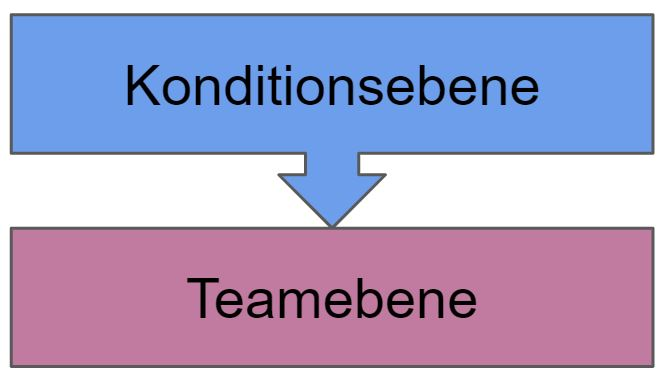
\includegraphics[scale=0.4]{Abbildungen/DifferentLevels.JPG}	
			\caption[Die Hierarchieebenen]{Die Hierarchie der Individualebene, Konditionsebene und Teamebene.}
			\label{DifferentLevels}
		\end{footnotesize}
	\end{figure}

\paragraph{Generelles Vertrauen}
Es wird der Zusammenhang zwischen dem \textit{generellen Vertrauen} und dem \textit{kognitiven Vertrauen} auf \textit{Konditionsebene} analysiert.
Es wird auf \textit{Teamebene} analysiert, ob ein Zusammenhang zwischen dem \textit{generellen Vertrauen} und der \textit{Teameffektivität} besteht.

\paragraph{Kognitives Vertrauen}
Es wird der Zusammenhang zwischen dem \textit{gebildeten kognitiven Vertrauen} und der \textit{Teameffektivität} auf \textit{Teamebene} analysiert.

\paragraph{Avatar-Darstellung}
Es wird der \textit{Unterschied} zwischen dem \textit{gebildeten kognitiven Vertrauen} bei unterschiedlichen Avatar-Konditionen auf \textit{Konditionsebene} analysiert.
Es wird der \textit{Unterschied} \textit{der Teameffektivität} bei unterschiedlichen Avatar-Konditionen auf \textit{Teamebene} analysiert.

Anhand des im Folgenden grafisch dargestellten Frameworks (siehe \textit{Abbildung \ref{Versuchshypothesen}}) wurden Hypothesen entwickelt, die im nächsten Kapitel genauer definiert und erklärt werden.

\begin{figure}[H]
		\begin{footnotesize}
			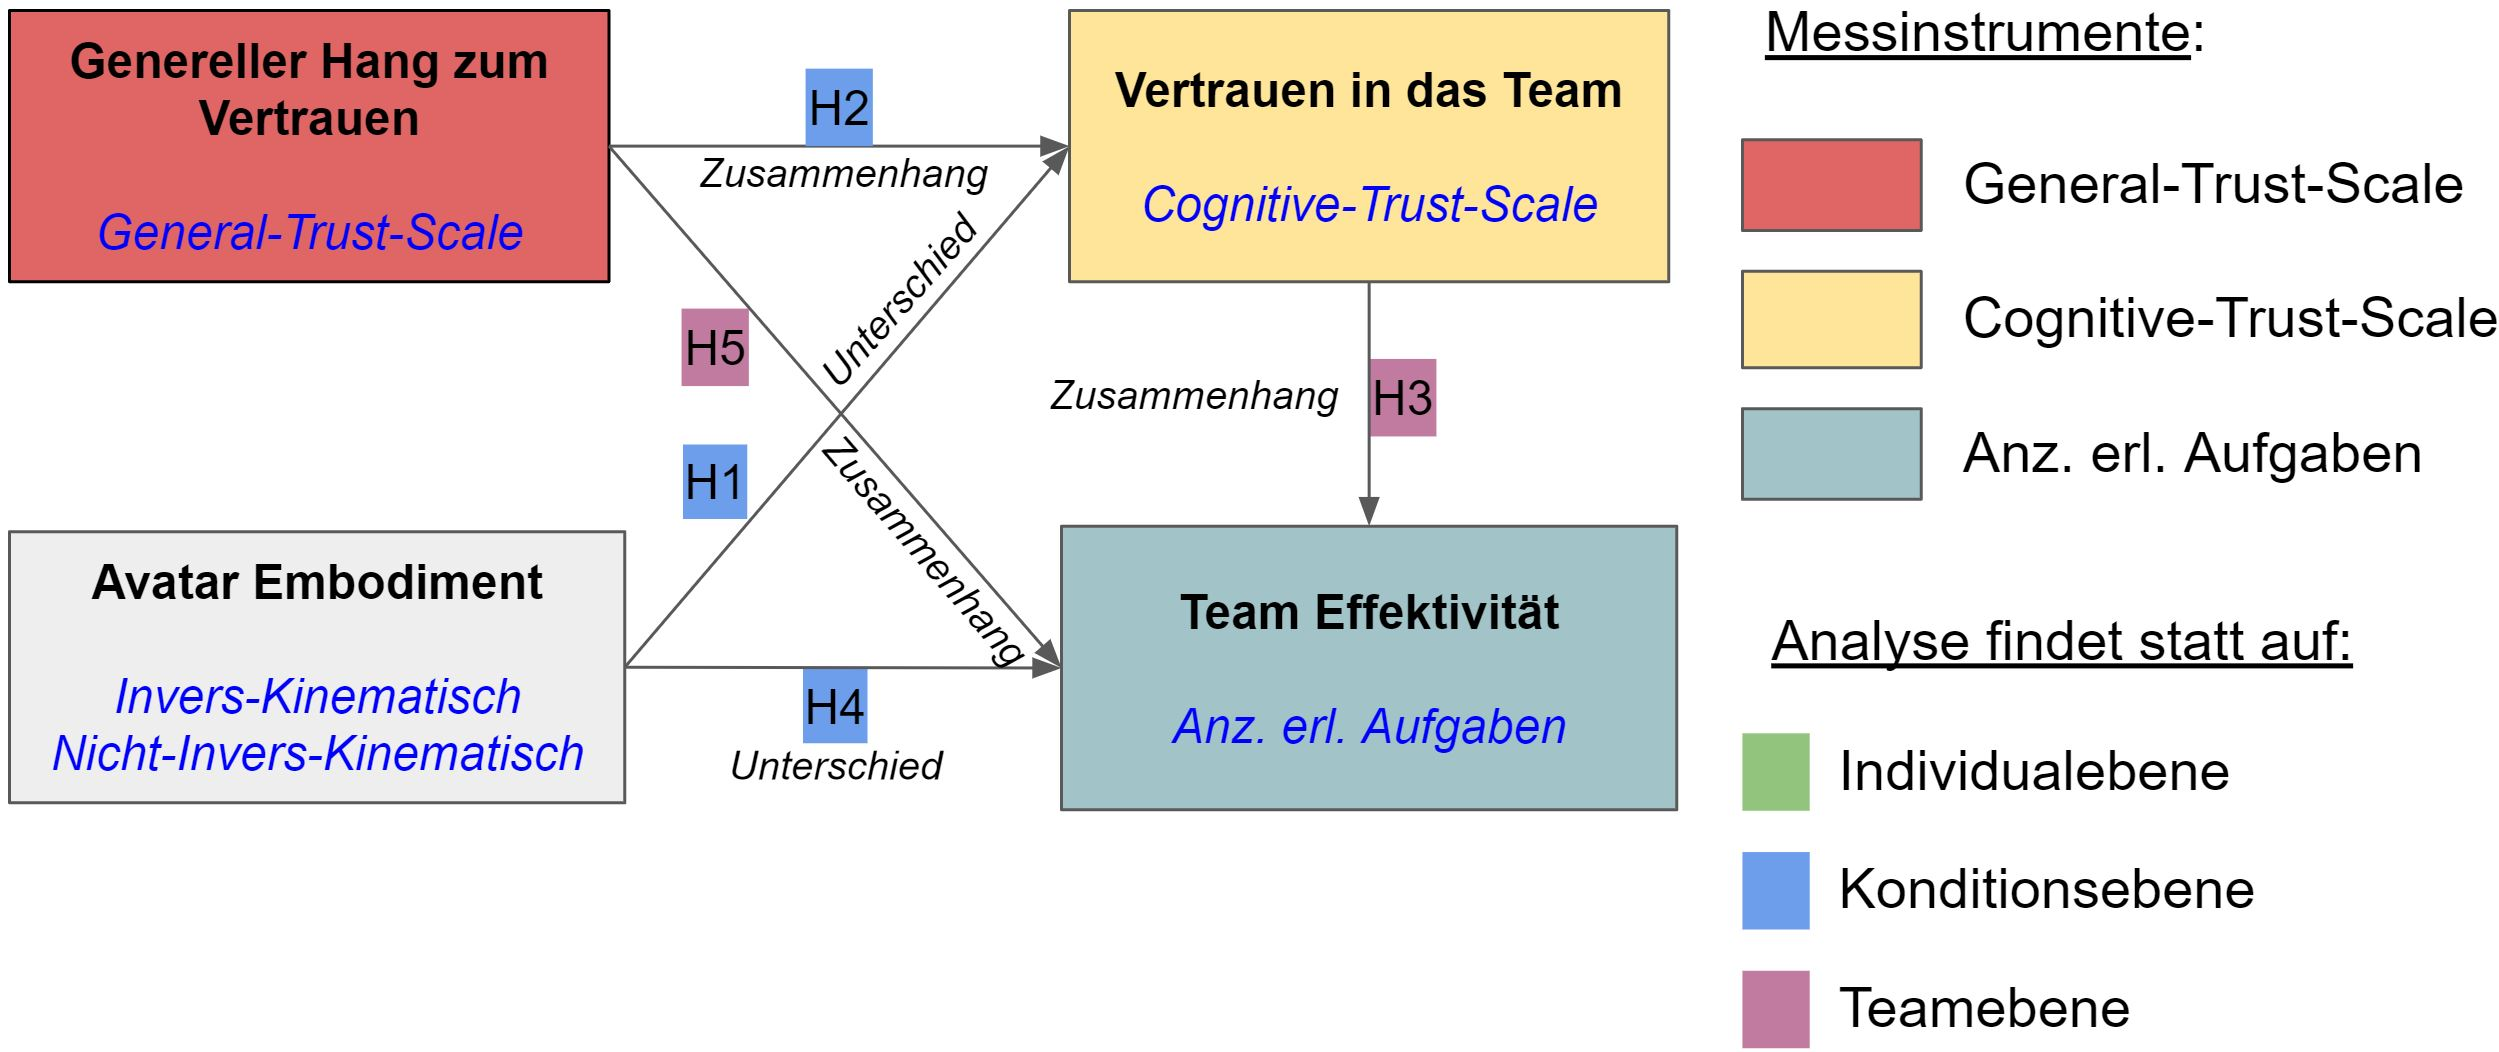
\includegraphics[width=\textwidth]{Abbildungen/Versuchshypothesen_02.JPG}		
			\caption[Das Framework der Versuchshypothesen]{Dieses Framework verdeutlicht, wie die Hypothesen zusammenhängen.}
			\label{Versuchshypothesen}
		\end{footnotesize}
	\end{figure}	

\newpage

%Da dieses Framework nicht validiert ist, kann es sein, dass die verschiedenen Faktoren nicht zu gleichen oder auch gar keinen Einfluss auf die Teameffektivität haben.

%\paragraph{Die Analyseebenen}
%Einige Variablen wurden in dieser Studie auf der Individualebene, auf der Konditionsebene oder auf der Teamebene gemessen.
%Konditionsebene bedeutet dabei, dass das die Ergebnisse zwischen der Kondition \ac{ik} sowie \ac{nik} aufgeteilt wurden, während auf der Individualebene alle Teilnehmer einzeln bewertet wurden. Die Teamebene teilt die Konditionen \ac{ik} und \ac{nik} zusätzlich noch in Teams von 3 Personen auf.  Alle Variablen, die auf der Individualebene gemessen wurden, haben eine Stichprobengröße $N = 30$, die auf dem Konditionsebene $ N = 15$ und die auf der Teamebene von $N = 5$.
%Die \textit{Tabelle \ref{MittelwerteUndCo}} zeigt eine Übersicht über die gemessenen Variablen, deren Mittelwerte, Standartabweichungen und die Anzahl der Teilnehmer der Messung.

\subsubsection{Die Versuchshypothesen}
\label{VersuchshypothesenAuflistung}

\paragraph{Hypothese 1}
\textit{Kognitives Vertrauen} wird in der Anfangsphase einer Teamgründung frühzeitig gebildet.
Der kognitive Vertrauensaufbau basiert auf der Wahrnehmung von Kompetenz und Zuverlässigkeit der Person gegenüber (siehe Kapitel \ref{Vertrauen als Zustand-Label}). Gleichzeitig haben Kategorisierungseffekte einen Einfluss auf die Vertrauensbildung (siehe Kapitel \ref{Vertrauen und virtuelle Teams}). Somit lässt sich die Vermutung aufstellen, dass ein \ac{ik} sowie ein \ac{nik} Avatar einen unterschiedlichen Einfluss auf die kognitive Vertrauensbildung besitzen (siehe Kapitel \ref{AvatarTrust}).
%Je realistischer und menschenähnlicher ein Avatar aussieht, desto mehr kognitives Vertrauen könnte in diesen gebildet werden, da sich die Teilnehmer eher vorstellen können mit realen Menschen zusammenzuarbeiten als nur mit Repräsentationen eines Individuums aus Pixeln. Diese Einschätzung teilen auch Riedl et al. \citep{riedl2014trusting}, nachdem sie herausfanden, dass es Personen leichter fällt einzuschätzen, wie vertrauenswürdig ein Mensch ist, wenn dieser ein menschenähnliches Gesicht besitzt.
Eine Analyse des \textit{kognitiven Vertrauens} auf \textit{Konditionsebene} soll feststellen, ob sich unterschiedliche Avatar-Konditionen auf die Wahrnehmung in die Fähigkeiten und die Zuverlässigkeit eines \textit{virtuellen Teams} im \ac{sve}, auswirken.
%Daher wird \textbf{Hypothese H1} wie folgt aufgestellt:
\begin{quote}
\textbf{H1$_{1}$}: Die Mittelwerte der erzielten \textit{kognitiven Vertrauenswerte} unterscheiden sich bei den Konditionen \ac{ik} und \ac{nik} signifikant voneinander.
%\textbf{H1$_{0}$}: Die Mittelwerte der erzielten \textit{kognitiven Vertrauenswerte} unterscheiden sich bei den Konditionen \ac{ik} und \ac{nik} nicht signifikant voneinander.
\end{quote}

\paragraph{Hypothese 2}
Diese Hypothese wird auf \textit{Konditionsebene} untersucht, um festzustellen, ob es unterschiedliche Zusammenhänge anhand einer Avatar-Kondition zwischen dem \textit{generellen Vertrauen} und dem \textit{kognitiven Vertrauen} gibt. Besitzt eine Person ein hohes \textit{generelles Vertrauen}, sollte diese auch ein hohes \textit{kognitives Vertrauen} aufgrund der Kurzlebigkeit eines \textit{virtuellen Teams} bilden (siehe. Kapitel \ref{Aufbau eines virtuellen Teams} und Kapitel \ref{Konstrukt des Vertrauens}).
Da ein starkes \textit{kognitives Vertrauen} in ein \textit{virtuelles Team} während der Neugründung im \ac{sve} wünschenswert ist, wird aus den vorherigen Erkenntnissen folgende Hypothese aufgestellt:
\begin{quote}
\textbf{H2$_{1}$}: Je höher der erzielte \textit{generelle Vertrauenswert} einer Person ist, desto höher ist der erzielte \textit{kognitive Vertrauenswert} einer Person.
%\textbf{H2$_{0}$}: Es besteht kein signifikanter Zusammenhang zwischen dem erzielten \textit{generellen Vertrauenswert} einer Person und dem erzielten \textit{kognitiven Vertrauenswert} einer Person.
\end{quote}

\paragraph{Hypothese 3}
% VGL : https://www.youtube.com/watch?v=SVuniaJXOoM&ab_channel=drfg2008
Aufgrund von Kategorisierungseffekten (siehe Kapitel \ref{Vertrauen und virtuelle Teams}) und der Annahme, dass mehr \textit{kognitives Vertrauen} die \textit{Teameffektivität} eines virtuellen Teams vorteilhaft beeinflusst (siehe Kapitel \ref{TEinVT}), wird die Hypothese 3 auf \textit{Teamebene} analysiert und wie folgt aufgestellt: 
%Ein starkes zwischenmenschliches Vertrauen in traditionell geformten Teams beeinflusst die \textit{Teameffektivität} des Teams positiv (siehe. Kapitel \ref{Konstrukt des Vertrauens}). Es wird davon ausgegangen, dass dies auch auf \textit{virtuelle Teams} zutrifft. 
%Je größer das \textit{kognitive Vertrauen} eines Teams, desto mehr können die einzelnen Teammitglieder ihre Ressourcen in die Teamarbeit einbringen (siehe. Kapitel \ref{TEinVT}). 
%Das \textit{kognitive Vertrauen eines Teams}, könnte sich somit auf die \textit{Teameffektivität} eines Teams auswirken. 
%Es wird die \textbf{Hypothese 3} wie folgt aufgestellt:
\begin{quote}
\textbf{H3$_{1}$}: Der Zusammenhang zwischen dem \textit{kognitiven Vertrauenswert von Teams} und der \textit{Teameffektivität von Teams} mit der Kondition \ac{ik} ist stärker als der von Teams mit der Kondition \ac{nik}.
%\textbf{H3$_{0}$}: Der Zusammenhang zwischen dem \textit{kognitiven Vertrauenswert von Teams} und der \textit{Teameffektivität von Teams} mit der Kondition \ac{ik} unterscheiden sich nicht signifikant von den Teams mit der Kondition \ac{nik}.
\end{quote}

\paragraph{Hypothese 4}
Es wird auf \textit{Konditionsebene} untersucht, ob unterschiedliche Avatar-Konditionen einen unterschiedlichen Einfluss auf die \textit{Teameffektivität} besitzen (siehe Kapitel \ref{Teameffektivität}).
%Unterschiedliche Avatar-Konditionen könnten einen Einfluss auf die \textit{Teameffektivität} eines Teams, aufgrund verschiedener besitzen (\textit{siehe Kapitel \ref{Teameffektivität}}). 
Um dies zu überprüfen, wird folgende Hypothese aufgestellt:
\begin{quote}
\textbf{H4$_{1}$}: Die Mittelwerte der \textit{Teameffektivität} unterscheiden sich bei den Konditionen \newline \ac{ik} und \ac{nik} signifikant voneinander.
%H4$_{0}$: Die Mittelwerte der \textit{Teameffektivität} unterscheidet sich bei den Konditionen \ac{ik} und \ac{nik} nicht signifikant voneinander.
\end{quote}

\newpage
\paragraph{Hypothese 5}
Virtuelle Teams sind gegebenenfalls von kurzer Dauer (siehe. Kapitel \ref{Aufbau eines virtuellen Teams}). Besitzt ein \textit{virtuelles Team} ein hohes \textit{generelles Vertrauen}, könnte sich dies aufgrund der kurzen Lebensdauer eines \textit{virtuellen Teams} sowie aufgrund von kognitiver, auf einer Kategorie basierten, schnellen Meinungsbildung positiv auf die \textit{Teameffektivität} auswirken. Demnach wird Hypothese 5 auf \textit{Teamebene} analysiert und wie folgt aufgestellt:
%Um zu untersuchen, ob die \textit{Teameffektivität} im Zusammenhang mit dem \textit{generellen Vertrauen} steht, wurde \textbf{Hypothese 5} aufgestellt:
\begin{quote}
\textbf{H5$_{1}$}: Der Zusammenhang zwischen dem \textit{generellen Vertrauenswert eines Teams} und der \textit{Teameffektivität eines Teams} mit der Kondition \ac{ik} ist stärker als der von Teams mit der Kondition \ac{nik}.
%\textbf{H5$_{0}$}: Der Zusammenhang zwischen dem \textit{generellen Vertrauenswert} eines Teams und der \textit{Teameffektivität} eines Teams mit der Kondition \ac{ik} unterscheidet sich nicht signifikant von den Teams mit der Kondition \ac{nik}.
\end{quote}
\newpage
\section{Vorgehensweise}

\subsection{Methodik}	
Das folgende Kapitel beschreibt das Forschungsdesign des Versuchs sowie die Methoden, die zur Datenerhebung herangezogen wurden.
\subsubsection{Forschungsdesign}

Um die beiden unabhängigen Variablen \textit{\ac{nik}} und \textit{\ac{ik}} innerhalb der Versuchsumgebung zu untersuchen, wird das \textit{A/B-Testing} in Kombination mit einem induktiven quantitativen Forschungsdesign gewählt.
Gruppe A bekommt dabei die Kondition \newline \textit{\ac{nik}} zugeteilt, während Gruppe B die Kondition \textit{\ac{ik}} zugeteilt wird. Diese Gruppeneinteilung der Probanden erfolgt nach dem Zufallsprinzip. 
Wie groß das \textit{gebildete Vertrauen in das Team} und die dadurch resultierende \textit{Teameffektivität} ist, soll durch die beiden Avatar-Konditionen \ac{ik} sowie \ac{nik} analysiert werden. Aufgrund des vorhandenen Lerneffekts können die Probanden nur einmal an der Studie teilnehmen.

%\paragraph{Between-Subject Forschungsdesign}
%Deshalb wurde ein \textit{Between-Subject Forschungsdesign} gewählt, bei dem jedem Versuchsteilnehmer einer der beiden Avatar-Konditionen zugeteilt bekommt.
%			\paragraph{Unabhängige Variablen}
%%Die unabhängigen Variablen sind der \dq{}\ac{ik}-Avatar\dq{} sowie der \glqq{}\ac{ik}-Avatar\dq{}. Durch diese beiden Variablen wurde im weiterem Versuchsverlauf versucht den Einfluss auf die abhängigen Variablen zu bestimmen.
%Für \textbf{Hypothese 1} wurde als unabhängie Variable das \textit{generelle Vertrauen} und als abhängige Variable das \textit{kognitive Vertrauen} gewählt.
%Für \textbf{Hypothese 2} wurde als unabhängie Variable die \textit{Avatarkondition} und als abhängige Variable das \textit{kognitive Vertrauen} gewählt.
%Für \textbf{Hypothese 3} wurde als unabhängie Variable das \textit{kognitive Vertrauen im Team} und als abhängige Variable die \textit{Teameffektivität} gewählt.
%Für \textbf{Hypothese 4} wurde als unabhängie Variable die \textit{Avatar-Kondition} und als abhängige Variable die \textit{Teameffektivität} gewählt.
%Für \textbf{Hypothese 5} wurde als unabhängie Variable das \textit{generelle Vertrauen} und als abhängige Variable die \textit{Teameffektivität} gewählt.

Die abhängigen Variablen werden im Folgenden aufgeführt:
\begin{itemize}
\item \textbf{Hang zum Vertrauen} Der Hang zum Vertrauen bezieht sich in dieser Studie darauf, wie sehr die Teilnehmer dazu neigen, anderen Personen einen Vertrauensvorschuss zu gewähren. Der Hang zum Vertrauen wird auch als \textit{generelles Vertrauen} bezeichnet \citep[S. 30]{mcallister1995affect} (\textit{vgl. Kapitel \nameref{Vertrauen}}).
\item \textbf{Kognitives Vertrauen} Das \textit{kognitive Vertrauen} bezieht sich auf die \textit{Überzeugung in die Fähigkeiten oder in die Zuverlässigkeit eines anderen} \citep[S. 30]{mcallister1995affect} (\textit{vgl. Kapitel \nameref{Vertrauen}}).
\item \textbf{Teameffektivität} Die \textit{Teameffektivität} wird anhand der Anzahl der abgeschlossenen Runden im Team gemessen (\textit{vgl. Kapitel \nameref{Avatare}}).
\end{itemize}

Zusätzlich wurde der Unterschied zwischen den \textit{Avatar-Konditionen} bei der \textit{wahrgenommenen Teameffektivität}, der \textit{Präsenz}, der \textit{subjektiv wahrgenommenen Arbeitsbelastung}, der \textit{Team-Kommunikation} sowie der \textit{Co-Präsenz} analysiert.
				
%	\paragraph{Residuuen}
%\begin{itemize}
%\item \textbf{Kommunikation mit dem Spectator} Da die Teilnehmer mit dem Spectator in Verbindung stehen, kann es sein, dass die Teilnehmer durch eine plötzlich auftretende Stimme einen \ac{bip} erfahren.
%\item \textbf{Farbe und Geschlecht der Avatare} Personen verbinden mit verschiedenen Farben verschiedene Eigenschaften. Es wurde durch die Farbe schwarz so neutral wie möglich zu bleiben.
%\item \textbf{Grad der Gamification} Einige Spieler könnten das gesamte Experiment \ac{vr} als Spiel zur Unterhaltung empfinden, was das Ergebnis beeinflussen könnte. 
%\end{itemize}				

			\subsubsection{Datenerhebungsmethoden}
Es wurden zwei Fragenbögen an die Teilnehmer verteilt. Der erste Fragenbogen (siehe \textit{Anhang \ref{Pre-Questionnaire}}) wurde vor dem Experiment ausgefüllt. In diesem wurden allgemeine demografische Fragen über \textit{die Person} sowie über eventuelle \textit{gesundheitliche Beschwerden} und die schon vorhandenen \textit{VR Erfahrungen} gestellt. Der zweite Fragebogen (siehe \textit{Anhang \ref{Post-Questionnaire}}) wurde nach der Durchführung des Experiments im \ac{sve} ausgefüllt. Er beinhaltet Fragen über das \textit{generelle Vertrauen}, das \textit{kognitive Vertrauen}, die \textit{Kommunikationsqualität}, \textit{die wahrgenommene Teameffektivität}, die \textit{Beanspruchung}, die \textit{Präsenz} sowie die \textit{Co-Präsenz}. 
Es wurden nur vollständig ausgefüllte Fragebögen zur Datenanalyse herangezogen. \\
				
		\paragraph{Demografie-Fragebogen}
Bevor der Versuch stattfinden konnte, mussten die Teilnehmer einen Demografie-Fragebogen ausfüllen. Dieser diente allgemein der Erfassung demografischer Merkmale wie z.B. das Alter, das Geschlecht und der Bildungsstand. Weiterhin wurde der demografische Fragebogen dazu genutzt, die bisher vorhandene VR-Erfahrung, die PC- und Internetaffinität sowie die Videospielerfahrung der einzelnen Probanden besser einschätzen zu können (siehe \textit{Anhang \ref{Pre-Questionnaire}}).

		\paragraph{General-Trust-Scale}
Der General-Trust-Scale ($\alpha =,91$) \citep{couch1996assessment} wurde eingesetzt, um den generellen Vertrauenswert der einzelnen Teilnehmer zu messen. Er besteht aus 20 Items. Dazu zählen beispielsweise: \glqq{}Ich neige dazu, andere zu akzeptieren\dq{} oder \glqq{}Meine Beziehungen zu anderen werden durch Vertrauen und Akzeptanz charakterisiert\dq{}. Die Items werden mit einer 7-Point-Likert-Skala von 1: \glqq{}Ich stimme gar nicht zu\dq{} bis zu 7: \glqq{}Ich stimme voll zu\dq{} gemessen. Der General-Trust-Scale Fragebogen ist ein Auszug aus dem \textit{Trust-Inventory} von Couch et al. (siehe \textit{Anhang \ref{Post-Questionnaire - Generelles Vertrauen}}). Höhere Werte spiegeln ein höheres Grundlevel an Vertrauen wider. Einige Fragen wurden in diesem Fragebogen invertiert gestellt und es wurde bei der Auswertung drauf geachtet diese korrekt auszuwerten.

%			
%			\textbf{The propensity to trust measure developed by Couch, Adams, & Jones (1996) was
%administered in order to gauge participants’ trusting dispositions. The Generalized Trust subscale
%of this measure was utilized for this study. It contains 20 items (e.g. “I have few difficulties
%trusting people”) and participants rated how strongly they agree with each statement on a 1
%(strongly disagree) to 7 (strongly agree) scale. See Appendix B for the full scale. The full trust
%inventory by Couch et al. (1996) also contains a Partner Trust subscale, but this was not relevant
%to the study as it pertains to trust of one’s romantic partner.}
%https://sci-hub.ren/10.1207/s15327752jpa6702_7
%\citep{couch1996assessment}

		\paragraph{Cognitive-Trust-Scale}
Der Cognitive-Trust-Scale ($\alpha =,91$) Fragebogen ist ein Auszug des von McAllister et al. \citep[S. 37]{mcallister1995affect} entwickelten Fragebogens. Er überprüft, wie viel \textit{kognitives Vertrauen} die Teilnehmer während des Versuchs aufbauen. Die Messgröße wird als kognitiver Vertrauenswert bezeichnet. Der Cognitive-Trust Fragebogen umfasst fünf Items. Dazu zählen beispielsweise: \glqq{}Diese Person geht an ihre Arbeit mit Professionalität und Hingabe heran\dq{} oder \glqq{}Andere Personen, die mit diesen Personen interagieren müssen, halten ihn/sie für vertrauenswürdig\dq{}. Die Antwortmöglichkeiten der im Fragebogen verwendeten 5-Point-Likert-Skala erstrecken sich von 1: \glqq{}Ich stimme gar nicht zu \dq{} bis 5: \glqq{}Ich stimme voll zu\dq{} (siehe \textit{Anhang \ref{Post-Questionnaire - Kognitives Vertrauen}}). Höhere Werte spiegeln ein höheres Grundlevel an kognitivem Vertrauen wider.

%			\textbf{After each bomb was completed (successfully or not), participants filled out a cognitive trust scale developed by Wildman et al. (2009) and based on the trust theory of Lewicki, McAllister, & Bies (1998). This 8-item scale taps into participants’ trust attitudes and each item is rated on a 5-point scale from “not at all” to “very much so”. While this measure has not yet been published, it has been validated in both lab and field samples and has shown utility in prior teamwork research Lazzara, 2013; Wildman, 2011. Appendix C contains the full scale}
%\citep{mcallister1995affect}

		\paragraph{Communication-Scale}
Gonzales-Rom et al. \citep[S. 1049]{gonzalez2014climate} entwickelten 2004 einen Fragebogen, um die \textit{Qualität von Teamkommunikation} ($\alpha =,76$) zu messen. Dieser Fragebogen umfasst fünf Items mit dem 5-Point-Likert-Skala von 1: \glqq{}Gar nicht\dq{} bis 5: \glqq{}Sehr\dq{}. Die Fragen sind alle nach demselben Prinzip aufgebaut, sodass jeweils nur das Ende einer Frage abgeändert wird: \glqq{}In welchem Umfang war die Kommunikation zwischen Ihnen und Ihrem Team \textit{KLAR / EFFEKTIV / ABGESCHLOSSEN / FLÜSSIG / ZUM RICHTIGEN ZEITPUNKT\dq{}} (siehe \textit{Anhang \ref{Post-Questionnaire - Teamkommunikation}}). Höher angegebene Werte spiegeln eine besser empfundene Teamkommunikation wider.
%			After the experimental portion was completed, participants completed another set of measures. First, participants completed the Communication Quality Scale developed by Gonzalez-Roma & Hernandez 2014. This scale contains 5 items that assess participants perceptions of their teams communication quality, rated on a 1 to 5 scale. The full measure is available in Appendix D
%\citep[S. 1049]{gonzalez2014climate}

		\paragraph{Team-Effectivness-Scale}
Gibson et al. \citep[S. 469]{gibson2003team} entwickelten 2003 einen Fragebogen, der die \textit{wahrgenommene Teameffektivität} ($\alpha =,62-,88$) misst. In dieser Studie wurde ein Auszug des Fragebogens verwendet. Er misst das \textit{subjektive Ausmaß der wahrgenommenen Teameffektivität} und umfasst fünf Items mit einer 7-Point-Likert-Skala 1: \glqq{}Ich stimme gar nicht zu\dq{} bis 7: \glqq{}Ich stimme voll zu\dq{} (siehe \textit{Anhang \ref{Post-Questionnaire - Team-Effektivität}}). Einige Fragen wurden in diesem Fragebogen invertiert gestellt und es wurde bei der Auswertung drauf geachtet diese korrekt auszuwerten. Je höher die angegebenen Werte des Team-Effectiveness-Scale sind, desto höher ist das Likert-Item zu bewerten.

%quality dimension is the extent to which the team produces error-free work.
%			\textbf{Next, participants completed a 5-item team effectiveness measure. This measure is
%comprised of the Quality subscale from Gibson, Zellmer-Bruhn, and Schwab's (2003) Team
%Outcome Effectiveness survey. Participants rated their agreement with each of the five items on
%a 1 to 7 scale. The team effectiveness measure is available in Appendix E.
%Last, participants indicated whether or not they were already familiar with their
%teammate. If so, they were also asked to indicate approximately how many years they had known
%their teammate, and how often they communicated with the teammate. Finally, teams were
%prompted to write a few sentences about why they thought their team performed the way it did.
%Effectiveness Measures} \citep[S. 469]{gibson2003team}

		\paragraph{NASA-TLX}
Der NASA-TLX ($\alpha =,84$) erfragt die allgemeine Belastung der Probanden, die sie während des Experiments empfunden haben. Dafür werden sechs Belastungsbereiche auf einer 21-Punkte Skala abgefragt. Diese beinhalten die mentale Anforderung, die physische Anforderung, die zeitliche Anforderung, die Leistung, die Anstrengung und die Frustration des Probanden \citep{NASATLX}.
Der originale NASA-TLX Fragebogen besitzt eine kontinuierliche Skala. Dies war über einen Online-Fragebogen jedoch nicht realisierbar, weshalb die Werteskala für die Onlineversion angepasst wurde. Diese Werteskala umfasst im abgeänderten Fragebogen 1: \glqq{}Wenig\dq{} über 11: \glqq{}Mittel\dq{} bis 21: \glqq{}Viel\dq{} (siehe \textit{Anhang \ref{Post-Questionnaire - NASA-TLX}}). Niedrigere Werte des NASA-TLX spiegeln eine gering empfundene Belastung wider.

		\paragraph{Igroup Presence Questionnaire(IPQ)}
Der IPQ ($\alpha =,85$) dient zur \textit{Messung des Präsenz-Gefühls} in einer virtuellen Umgebung. Er misst, inwieweit sich der Nutzer in der virtuellen Umgebung anwesend fühlt, inwieweit der Nutzer seine Aufmerksamkeit der virtuellen Umgebung schenkt und wie real die virtuelle Umgebung dem Nutzer erschien. Der IPQ umfasst 14 Items mit einer 7-Point-Likert-Skala (siehe \textit{Anhang \ref{Post-Questionnaire - IPQ}}). Je höher die angegebenen Werte sind, desto höher ist das Gefühl der Präsenz der Person. Einige Fragen wurden in diesem Fragebogen invertiert gestellt und es wurde bei der Auswertung drauf geachtet, diese korrekt auszuwerten.
		
		\paragraph{Co-Presence-Questionnaire}
Mithilfe des \textit{Co-Präsenz-Fragebogens} können die \textit{selbst gemeldete Co-Präsenz} ($\alpha =,78$), die \textit{wahrgenommene Präsenz des anderen} ($\alpha =,90$), die \textit{Telepräsenz} ($\alpha =,88$) sowie die \textit{soziale Präsenz} ($\alpha =,82$) ermittelt werden. Die \textit{selbst gemeldete Co-Präsenz} sowie die \textit{wahrgenommene Präsenz des anderen} werden mittels einer 5-Point-Likert-Skala gemessen. Die \textit{Telepräsenz} wird mit einer 7-Point-Likert-Skala ermittelt. Die \textit{soziale Präsenz} wird im originalen Fragebogen von Nowak et al. mittels einer kontinuierlichen Skala gemessen. Da dies mit dem Online-Fragebogen nicht realisierbar war, wurde stattdessen eine Likert-Skala von 1 bis 10 verwendet (\citep[S. 487]{nowak2003effect}) (siehe \textit{Anhang \ref{Post-Questionnaire - Co-Presence}}). Einige Fragen wurden in diesem Fragebogen invertiert gestellt und es wurde bei der Auswertung drauf geachtet diese korrekt auszuwerten. Höhere Werte spiegeln eine höheres Gefühl der verschiedenen Co-Präsenzen dar.
\clearpage
\newpage
\begin{table}
		\centering\footnotesize\setstretch{1.2}
		\caption[Verwendete Metriken des Fragbogens]{Verwendete Metriken der Fragebögen.}
		\label{wasWurdeGemessen}
	\begin{tabular}{| p{3.5cm} | p{3.5cm} | p{3.0cm} | p{2.0cm} |  p{1.7cm} |}
\hline
\underline{Was wurde gemessen?} & \underline{Definition} & \underline{Metrik} & \underline{Autoren} &  \underline{Cronbachs $\alpha$}\\
    
    \hline
\multirow{2}{3.5cm}{Generelles Vertrauen}
	&Genereller Vertrauensvorschuss eines Individuums & Teilauszug des Trust-Inventorys - \textit{Generalized-Trust-Scale} \newline \textit{Siehe \textit{Tabelle \ref{Post-Questionnaire - Generelles Vertrauen}}} \newline &Couch, Adams, Jones (1996) \citep{couch1996assessment} & $.91$ \\
	&\,& 7-Point-Likert-Scale & &\, \\

    \hline
\multirow{2}{3.5cm}{Kognitives Vertrauen}
	&Überzeugung in die Fähigkeiten und in die Zuverlässigkeit des Teams& \textit{Cognitive-Trust-Scale} \newline \textit{Siehe \textit{Tabelle \ref{Post-Questionnaire - Kognitives Vertrauen}}} & McAllister, Daniel J. (1995) \citep{mcallister1995affect} & $.91$ \\
	&\,& 5-Point-Likert-Scale & &\, \\
    
    \hline
\multirow{2}{3.5cm}{Team-Kommunikation}
	&Wahrgenommene Kommunikationsqualität des Teams & \textit{Communication-Quality-Scale} \newline \textit{Siehe \textit{Tabelle \ref{Post-Questionnaire - Teamkommunikation}}} & Gonzalez-Roma, Hernandez (2014) \citep[S. 1049]{gonzalez2014climate} & $.76$ \\
	&\,& 5-Point-Likert-Scale & &\, \\
    
    \hline
\multirow{2}{3.5cm}{Wahrgenommene Teameffektivität}
	&Wahrgenommenes Ausmaß der Qualität der Aufgabenerledigung des Teams & Teilauszug des \textit{Team-Effectiveness-Scale} \newline \textit{Siehe \textit{Tabelle \ref{Post-Questionnaire - Team-Effektivität}}} & Gibson et. al (2003) \citep[S. 469]{gibson2003team} & $.62-.88$ \\
	&\,& 7-Point-Likert-Scale & &\, \\
    
    \hline
\multirow{2}{3.5cm}{Teameffektivität} & Messung der abgeschlossenen Runden des Teams während des Experiments & Abgeschlossene Runden &  &\\    
    
    \hline
\multirow{2}{3.5cm}{Subjektiv-wahrgenommene Arbeitsbelastung}
	&Der NASA-TLX misst die subjektiv wahrgenommene Arbeitsbelastung sowie Effektivität & \textit{NASA-TLX} \newline \textit{Siehe \textit{Tabelle \ref{Post-Questionnaire - NASA-TLX}}} & \citep{NASATLX} & $.84$\\
	&\,& Kontinuierliche Skala umgewandelt in 21-Point-Likert-Scale& &\, \\
    
    \hline
\multirow{2}{3.5cm}{Gefühl der Präsenz}
	&Der IPQ dient der Messung des Präsenz Gefühls in einer virtuellen Umgebung & \textit{Igroup Presence Questionnaire(IPQ)} \newline \textit{Siehe \textit{Tabelle \ref{Post-Questionnaire - IPQ}}} & \citep{IPQ} & $.85$\\
    &\,& 7-Point-Likert-Scale & &\, \\
    
    \hline
\multirow{2}{3.5cm}{Selbst wahrgenommene Co-Präsenz \newline \newline Wahrgenommene Präsenz des anderen \newline \newline Telepräsenz \newline \newline soziale Präsenz}
	&Fragebogen von Nowak und Biocca zum Messen von Co-Präsenz \newline  \newline  \newline  \newline  \newline  \newline & \textit{Presence-Questionnaire} \newline \textit{Siehe \textit{Tabelle \ref{Post-Questionnaire - Co-Presence}}} \newline \newline 5;7;10-Point-Likert-Scale & Nowak und Biocca (2003) \citep[S. 487]{nowak2003effect} & $.78$ \newline \newline \newline $.90$ \newline \newline \newline $.88$ \newline \newline $.82$ \\
\hline
	\end{tabular}
\end{table}
\clearpage			

\subsection{Der Versuch}
Im Folgenden wird beschrieben, wie die Teilnehmer für diese Studie ausgewählt werden, wie der Versuch aufgebaut ist und wie er umgesetzt wird.
	\subsubsection{Teilnehmerfindung}
Die Teilnehmer werden über zwei Wege akquiriert. Zum einen werden im Bekanntenkreis Personen angesprochen, denen die notwendige Hardware zur Verfügung gestellt wird. Zum anderen werden in verschiedenen Foren (z.B. VRForum.de, Computerbase.de, Hardwareluxx.de, etc.) in Form eines extra dafür angelegten Threads Teilnehmer gesucht, die an der Studie teilnehmen wollen. Weiterhin werden Teilnehmer mithilfe verschiedener sozialer Netzwerke mit einem Bezug zu VR sowie zufälliger WhatsApp-Chatgruppen mit 50 oder mehr Mitgliedern akquiriert. Da der gesamte Versuch, die Fragebögen sowie das Erklärvideo auf deutscher Sprache erstellt wurde, findet die Teilnehmerfindung nur im deutschsprachigen Raum statt.

	\subsubsection{Allgemeiner Versuchsablauf}
Zunächst wird jedem Team entweder die Kondition \ac{ik} oder \ac{nik} zugeordnet. Es gab fünf Teams mit der Kondition \ac{ik} sowie fünf Teams mit der Kondition \ac{nik}.
Es werden jeweils drei Personen in einem Zeitslot untergebracht, um ein Team zu bilden. Insgesamt nehmen somit drei Personen an einem Versuch zur selben Zeit mit derselben Kondition teil. Die Teilnehmer werden sich untereinander \textit{nicht} Face-to-Face vorgestellt und sehen sich während des gesamten Experiments nur als Repräsentation eines Avatars im \ac{sve}. 
Ein Zeitslot wird auf 35 Minuten festgelegt und teilt sich auf in
		\begin{itemize}
			\item 5 Minuten Pre-Questionnaire,
			\item 5 Minuten Videoerklärung,
			\item 10 Minuten Versuchsdurchführung,
			\item 15 Minuten Post-Questionnaire.
		\end{itemize}
Jeder Teilnehmer bekommt zu Beginn seines Zeitslots einen Pre-Questionnaire ausgehändigt, den er selbstständig ausfüllt. Alle Teilnehmer schauen sich anschließend ein Erklärvideo (siehe \textit{Anhang \ref{Erklärvideo}}) über das Experiment an, in dem alle relevanten Mechaniken und Funktionsweisen sowie der grobe Spielablauf erklärt werden. Durch das Erklärvideo wird sichergestellt, dass alle teilnehmende Person denselben Informationsgehalt über die Art und Weise des Ablaufs des Experiments besitzen. Alle Mitglieder eines Teams starten dadurch mit einem einheitlichen Wissensstand. Nachdem alle Personen die Videoerklärung angeschaut haben, beginnt das Experiment. Dazu starten die jeweiligen Teilnehmer die Anwendung. Es wird sich automatisch mit dem Online-Server des \ac{sve} verbunden. Die Teilnehmer haben nun 10 Minuten Zeit, möglichst viele Runden im Team zu absolvieren. Am Ende der Versuchsdurchführung wird ein Post-Questionnaire ausgeteilt, den die Teilnehmer ausfüllen müssen. Die maximale Versuchsdauer nach Start der Anwendung beträgt exakt 10 Minuten (600 Sekunden) und es können maximal 15 Runden absolviert werden. Die Runden werden dabei inkrementell schwieriger, da in jeder dritten Runde jeweils ein Symbol in den Pool der zu erratenden Symbole hinzukommt.

	\subsubsection{Versuchsaufbau}

\begin{figure}[h]
		\begin{footnotesize}
			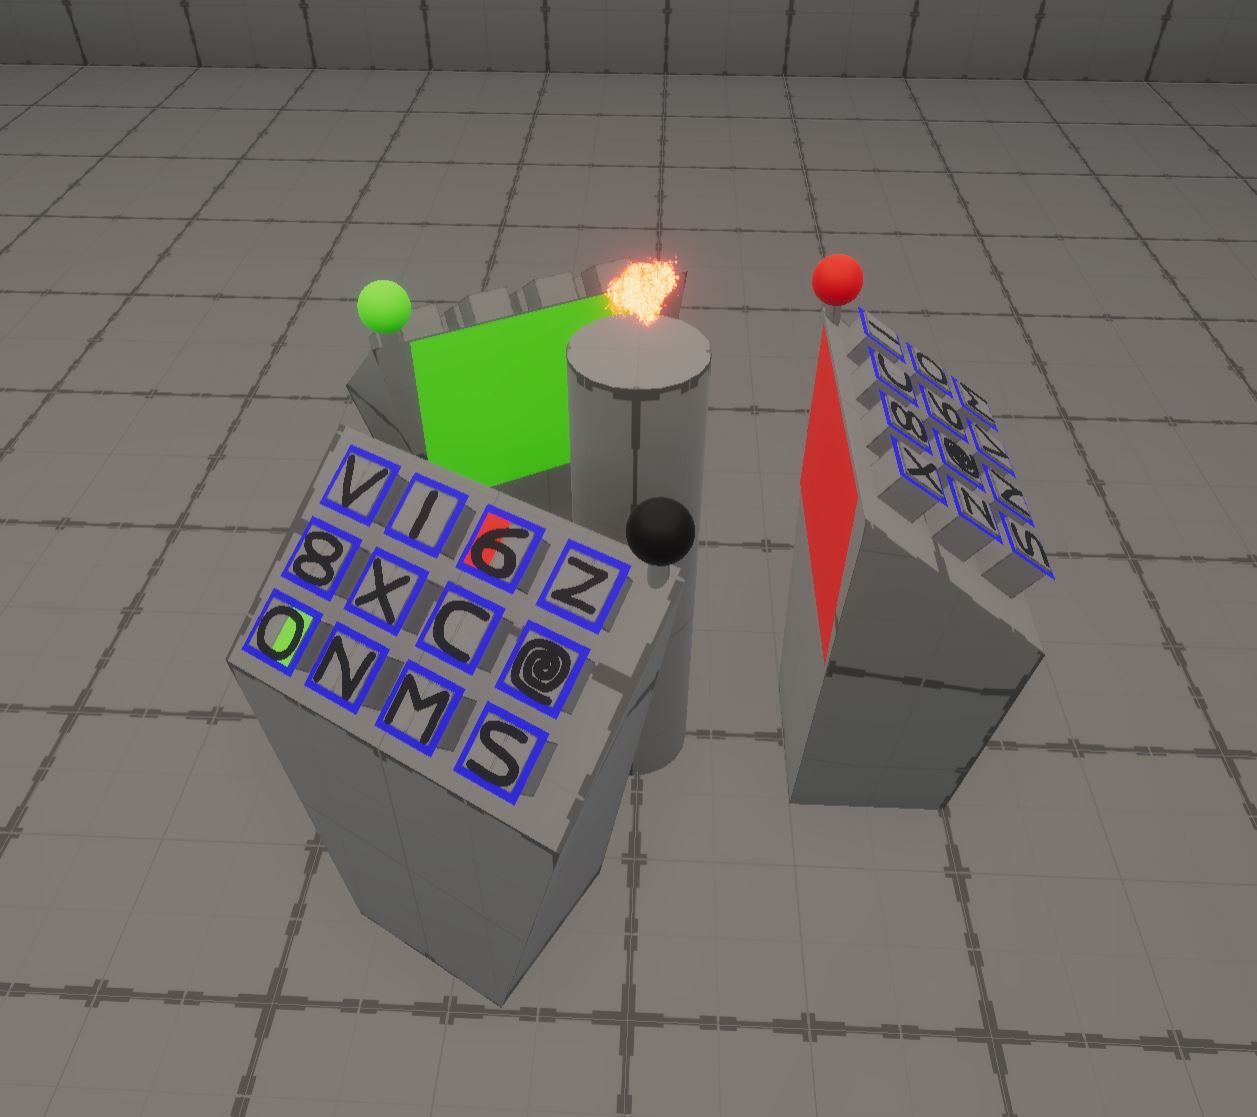
\includegraphics[width=\textwidth]{Abbildungen/Podeste.JPG}	
			\caption[Die Podeste der Teilnehmer]{Die Podeste der Teilnehmer des Experiments.}
			\label{Podeste}
		\end{footnotesize}
	\end{figure}

Um die Wahrscheinlichkeit zu erhöhen, dass auch in der Anfangsphase der Teamgründung eine soziale und keine arbeitsnahe, ergebnisorientierte Kommunikation stattfindet, wurde eine spielerische Umgebung geschaffen.

Jede Person benötigt (neben einem funktionsfähigen Computer) für das Experiment, entweder ein \textit{Oculus Rift/Rift S}, ein \textit{SteamVR} oder ein \textit{Windows Mixed-Reality} \ac{hmd} sowie zwei funktionsfähige Controller.

Dem Versuchsleiter ist es während der gesamten Anwendung möglich, die drei Teilnehmer durch einen separaten \textit{Spectator-Client} zu betreuen. Alle Teilnehmer können in der Anwendung durch das integrierte Mikrofon im \ac{hmd} mit dem Versuchsleiter sprechen und diesen hören. Wenn eine Person spricht, können die anderen zwei Teilnehmer diese nicht hören. Die Sprachkommunikation einer Person ist somit nur in Richtung des Versuchsleiters möglich, damit Störvariablen vermieden und die Integrität der Anonymität erhalten bleiben kann. Die Stimme des Versuchsleiters können alle Teilnehmer hören. Dies dient vor allem dazu, eventuell auftretende technische Schwierigkeiten schnell zu beheben und den Beginn sowie das Ende des Versuchs zu kommunizieren. Der Versuchsleiter gibt jedoch während der gesamten Dauer des Versuchs keine Hilfestellung.
Sind alle Teilnehmer bereit, werden sie vor ihr eigenes Podest (\textit{Abbildung \ref{Podeste}}) teleportiert. Durch den, für jeden sichtbar in der Mitte der Podeste platzierten Countdown, wird der baldige Beginn einer Runde eingeleitet. Bei jedem Start einer Runde, wird das Podest jeder teilnehmenden Person durch die Farbe Schwarz, Rot oder Grün markiert. Die Zuteilung der drei Farben ändert sich dabei nach jeder Runde. Die Teilnehmer können ihre eigene Farbe an einer Kugel und die Farbe der anderen Spieler zusätzlich an einem Viereck in der jeweils zugeteilten Farbe an den jeweiligen Podesten erkennen. Für den Programmcode siehe \textit{Anhang \ref{Programmcode}}.

	\subsubsection{Detaillierter Versuchsablauf}

Zu Beginn jeder neuen Runde können die Spieler die Zuteilung der Farben sehen und dadurch den Startspieler identifizieren. Dieser ist schwarz markiert und hat die Aufgabe, seinen Mitspielern die für ihn farblich gekennzeichneten Symbole zu erklären. Seine Mitspieler müssen die ihnen zugeteilten Symbole identifizieren und an ihrem Podest einloggen. Das Ziel ist, so viele Symbole wie möglich individuell korrekt zu erkennen, um dadurch gemeinsam in höhere Runden aufzusteigen.

Die Symbole auf dem Podest des schwarz markierten Spielers sind entweder durch die Farbe Grün, Rot oder Grün-Rot gekennzeichnet. Auf den Podesten der Mitspieler befinden sich ebenfalls Symbole, welche jedoch zufällig angeordnet sind und keine farblichen Markierungen haben (siehe \textit{Abbildung \ref{Podeste}}). Der schwarz markierte Spieler versucht nun, mittels Hand- und Armbewegung, den rot und grün markierten Mitspielern die Symbole, die in der jeweiligen Spielerfarbe vor ihm markiert sind, zu erklären. Meint der gerade angesprochene Mitspieler ein Symbol erkannt zu haben, loggt dieser das Symbol durch das Herunterdrücken des passenden Knopfes an seinem Podest ein. Hat sich ein Spieler während des Einloggens der Symbole verklickt oder möchte seine Angabe ändern, muss das Symbol durch erneutes Herunterdrücken ausgeloggt werden. Anschließend kann es erneut eingeloggt werden. 

Werden alle gekennzeichneten Symbole vom roten und grünen Spieler erkannt und eingeloggt, erscheint eine leuchtend grüne Kugel (\textit{Abbildung \ref{RoundFinished}}), die das Ende einer Runde anzeigt. Erscheint diese grüne Kugel nicht, ist noch ein Symbol falsch eingeloggt und der schwarz markierte Spieler muss noch einmal versuchen, die korrekten Symbole den jeweiligen Mitspielern aufzuzeigen. 
In der nächsten Runde wird ein anderer Spieler eindeutig mit Schwarz, Rot oder Grün markiert.
In der folgenden Runde erhält jeder Spieler wieder eine andere der drei Farben. Mit steigender Anzahl an erfolgreich bestandenen Runden müssen immer mehr Symbole richtig erkannt werden. 
Die \textit{Abbildung \ref{DetaillierterVersuchsablauf}} zeigt eine detaillierte Grafik zum Ablauf einer Runde.

	\begin{figure}[h]
		\begin{footnotesize}
		\centering
			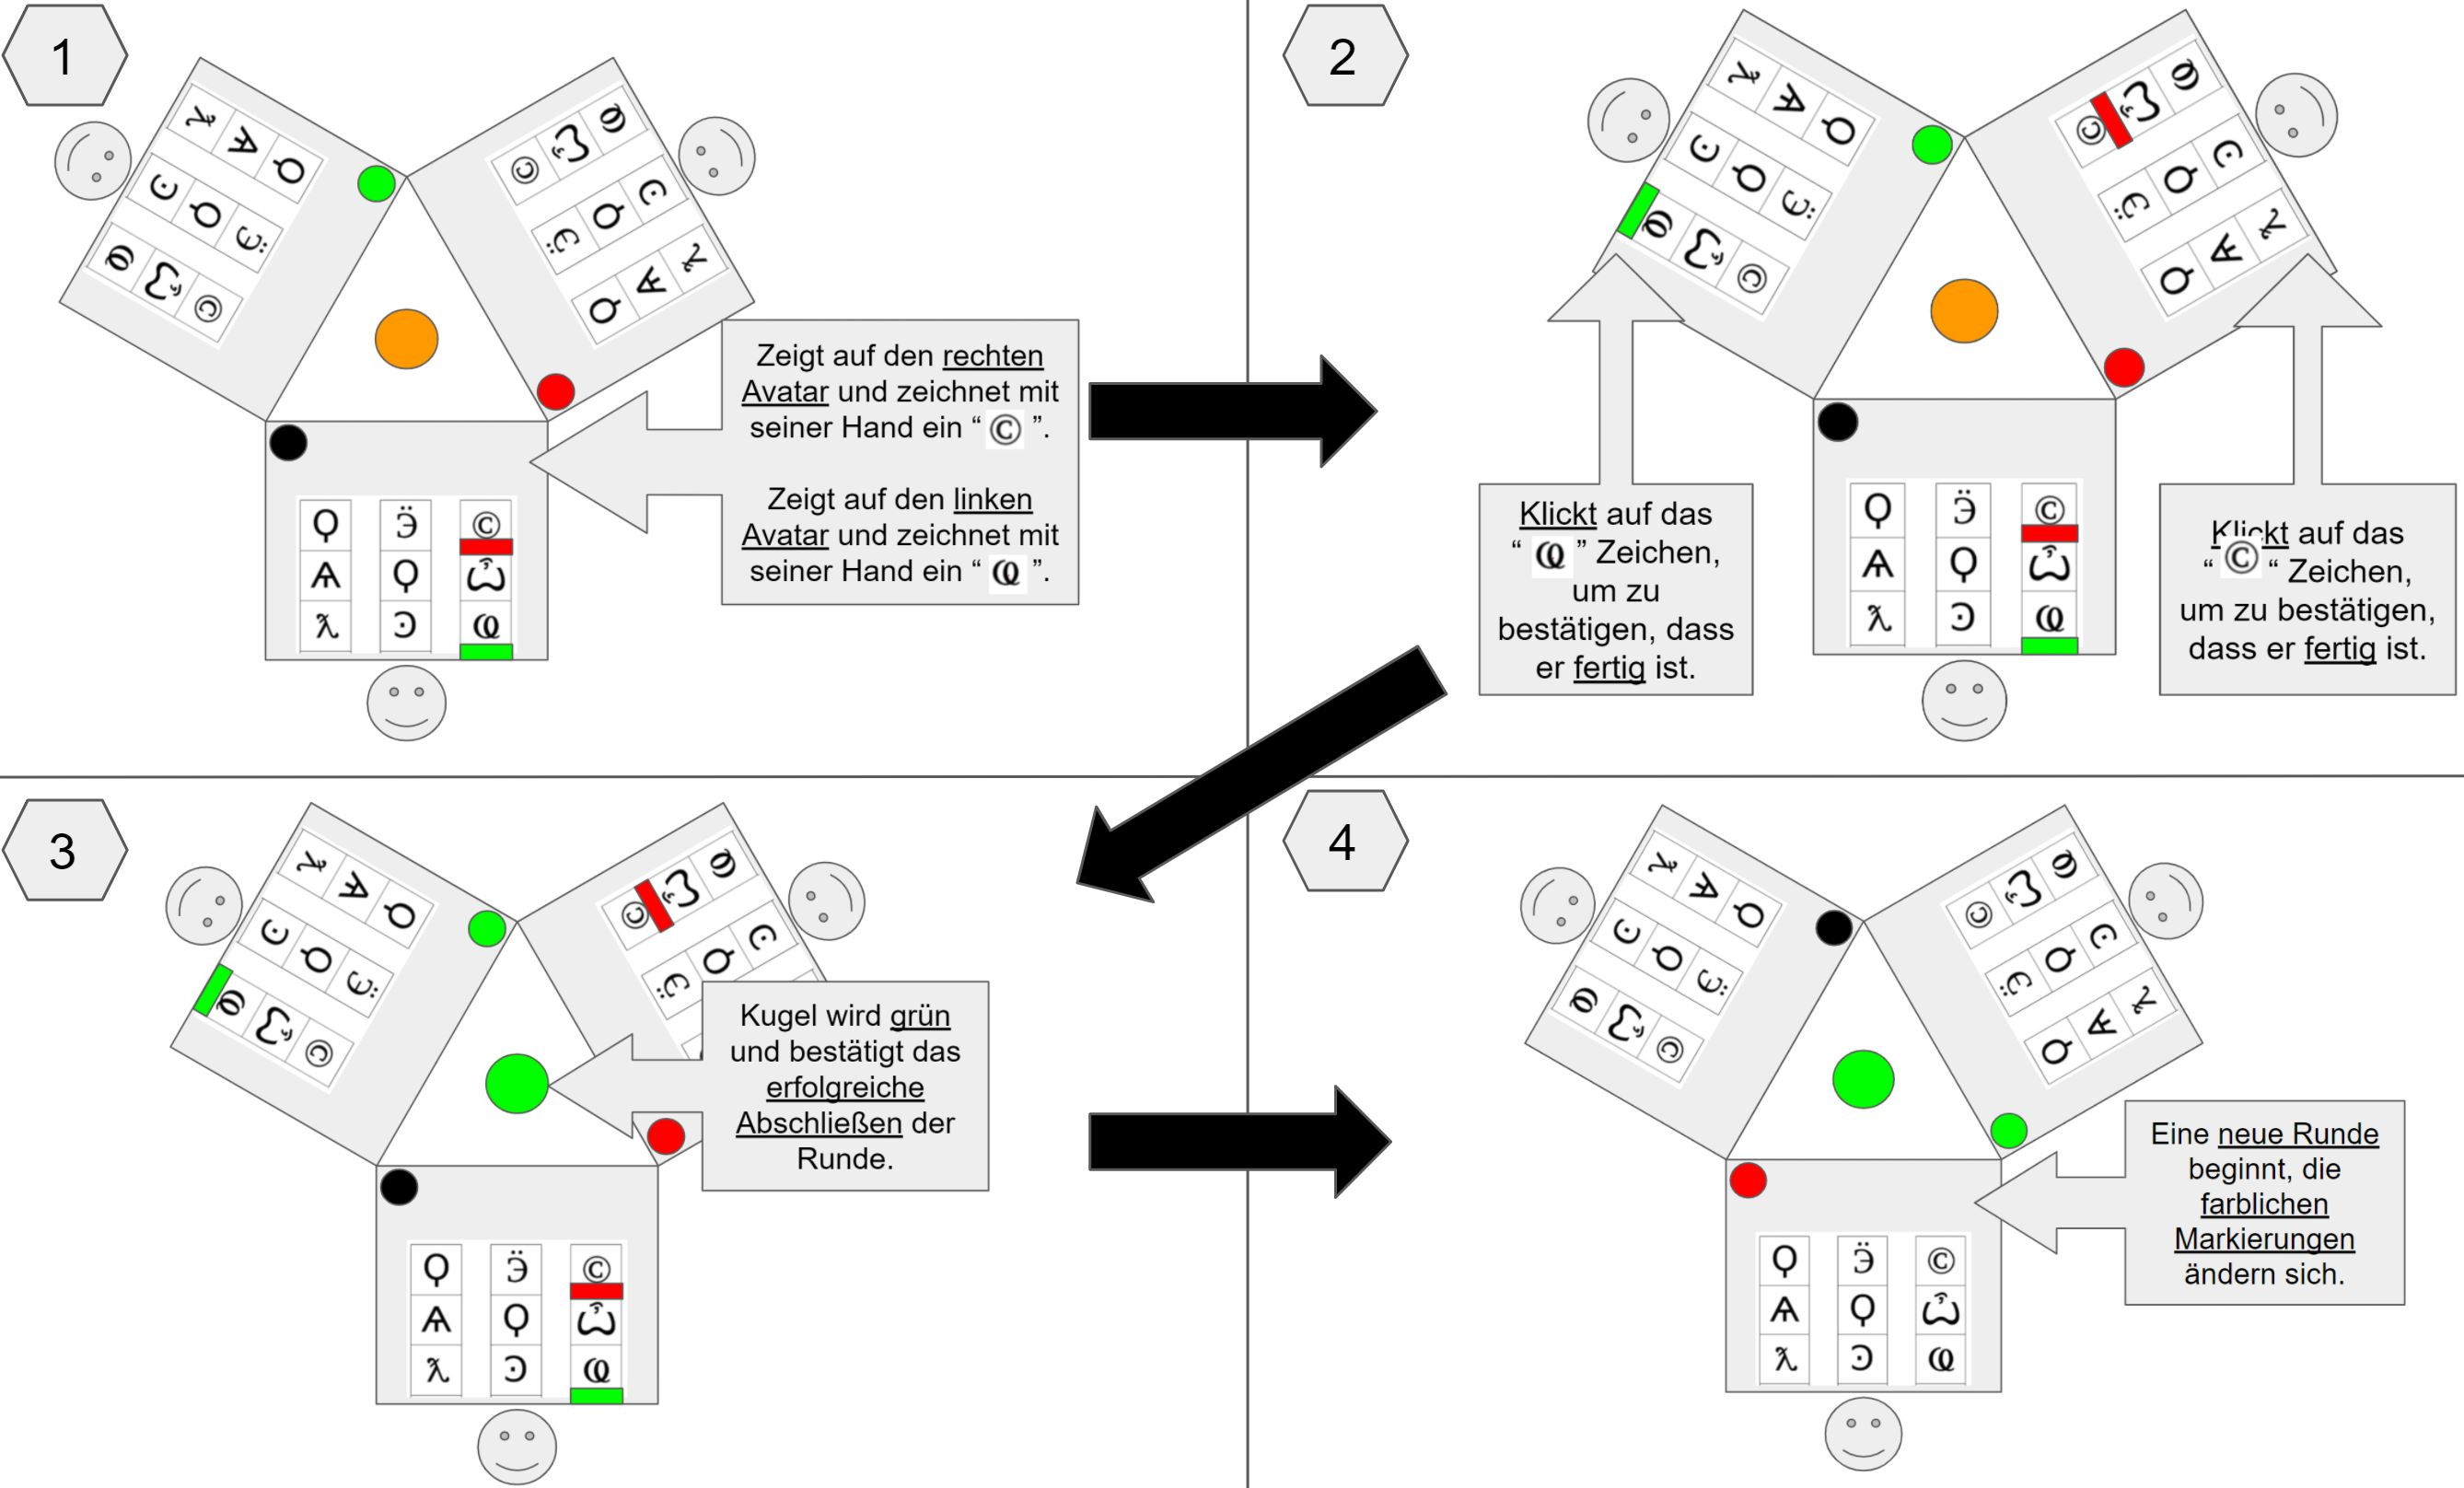
\includegraphics[scale=0.30]{Abbildungen/DetaillierterVersuchsablauf.JPG}		
			\caption[Darstellung des Versuchsablaufs]{Diese Grafik verdeutlicht den detaillierten Versuchsablauf.}
			\label{DetaillierterVersuchsablauf}
		\end{footnotesize}
	\end{figure}

	\subsubsection{Die verwendeten Avatare}
\label{IKNIK}
Die Avatare sind in dieser Studie als \textit{\ac{ik}} und \textit{\ac{nik}} implementiert. Als Grundlage der Visualisierung des \ac{ik}-Avatars dient eine Studie von Waldow et al. \citep{waldow2019investigating}, in der der Einfluss des Aussehens von Avataren in einem Augmented-Reality \ac{sve} untersucht wurde. Für die vorliegende Studie wurde lediglich die Farbe des Avatars \ac{ik} von Grün auf Schwarz geändert. 
Als Grundlage des Avatars \ac{nik} dient ein von dem Framework \textit{Normcore} bereitgestellter abstrakter Avatar.

Die Teams haben entweder die Kondition \ac{ik} oder \ac{nik}, sodass das Aussehen der Avatare innerhalb eines Teams immer identisch ist. Zur besseren Interaktion mit den Knöpfen sowie zur Vermeidung eines \textit{Break-In-Presence}, wird der \textit{eigene Avatar} nicht sichtbar für die Teilnehmer dargestellt. Jeder Teilnehmer sieht somit (unabhängig von der zugewiesenen Kondition) nur eine Repräsentation von menschlich wirkenden Händen ohne einen Körper. Die Person kann somit nur von dem Aussehen ihrer Teammitglieder auf die eigene Avatar-Darstellung schließen. \textit{Abbildung \ref{AvatareAussehen}} zeigt das Aussehen der Avatare dieser Studie.

	\begin{figure}[H]
		\begin{footnotesize}
		\centering
			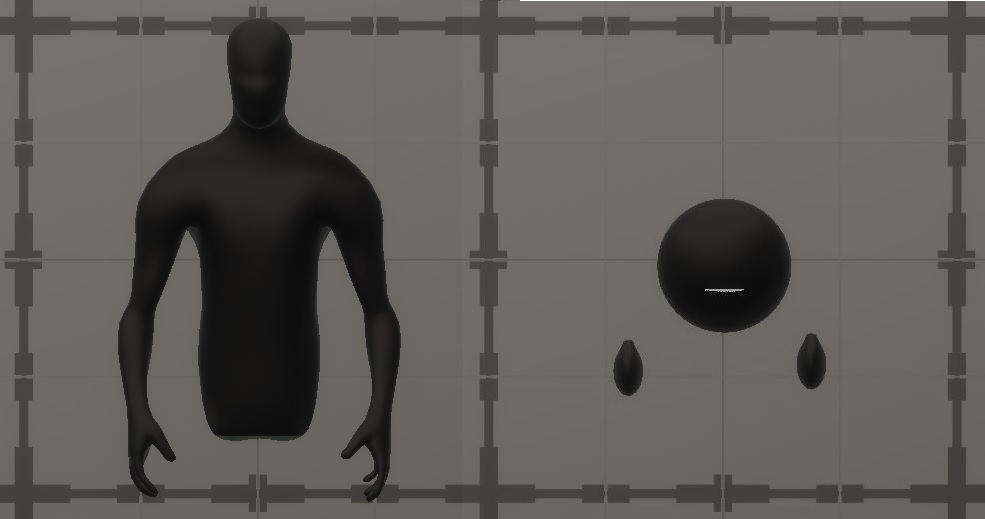
\includegraphics[width=\textwidth]{Abbildungen/Avatars.JPG}	
			\caption[Die verwendeten Avatare]{Die verwendeten Avatare : Links: IK-Avatar und rechts: Non-IK-Avatar.}
			\label{AvatareAussehen}
		\end{footnotesize}
	\end{figure}
	
		\paragraph{IK-Avatar}
Der invers-kinematisch dargestellte Avatar besitzt laut der Studie von Waldow \citep[S. 251]{waldow2019investigating} ein neutrales Erscheinungsbild. Der Avatar hat keine Augen, Mund, Haare oder Beine. Lediglich der Oberkörper, der Kopf sowie die Arme sind zu erkennen. Dieser Avatar besitzt somit keine Beine und schwebt mit dem Torso über dem Boden.
Die Handbewegungen, die Unterarmbewegungen, die Oberarmbewegungen sowie die Kopf- und Torsorotation des Avatar \ac{ik} werden invers-kinematisch dargestellt. Die Positions- und Rotationsdaten für den Kopf und den Oberkörper werden über das \ac{hmd} gewonnen. Die Positions- und Rotationsdaten der Arme werden über die beiden Controller gewonnen. Der Kopf des Avatars besitzt einen horizontalen Bewegungsbereich von 90$^\circ$. Wenn der Kopf diesen Bereich verlässt, rotiert der Oberkörper in Richtung der aktuellen Blickrichtung des Avatars. Der Oberkörper des Avatars folgt der Rotation des Kopfes also nicht simultan. Zusammen mit menschlichen Motion-Capture-Daten einer Leerlaufanimation wurde so eine plausible menschliche Bewegung erzeugt \citep[S. 251]{waldow2019investigating}.

		\paragraph{Non-IK-Avatar}
Der \ac{nik}-Avatar besteht aus einer Kugel mit Mund sowie einer Repräsentation der linken und der rechten Hand. Durch den fehlenden Oberkörper und die fehlenden Beine, schwebt der Avatar über dem Boden. Der Kopf ist frei beweglich und unabhängig von den Händen. Der Mund des Avatars bewegt sich nicht, sondern dient am Kopf als Orientierungspunkt. Dadurch kann ausgemacht werden, in welche Richtung der Kopf des Avatars gedreht ist. Die Positions- und Rotationsdaten für den Kopf werden über das \ac{hmd} gewonnen. Die Positions- und Rotationsdaten für die Hände werden über die beiden Controller gewonnen.\\
\textit{Abbildung \ref{AvatareImEinsatz}} zeigt beide Avatar-Konditionen \ac{ik} (a) und \ac{nik} (b) während der Versuchsdurchführung im Spectatorview.
\newpage

\begin{figure}[h]
  \centering
  \subfloat[][]{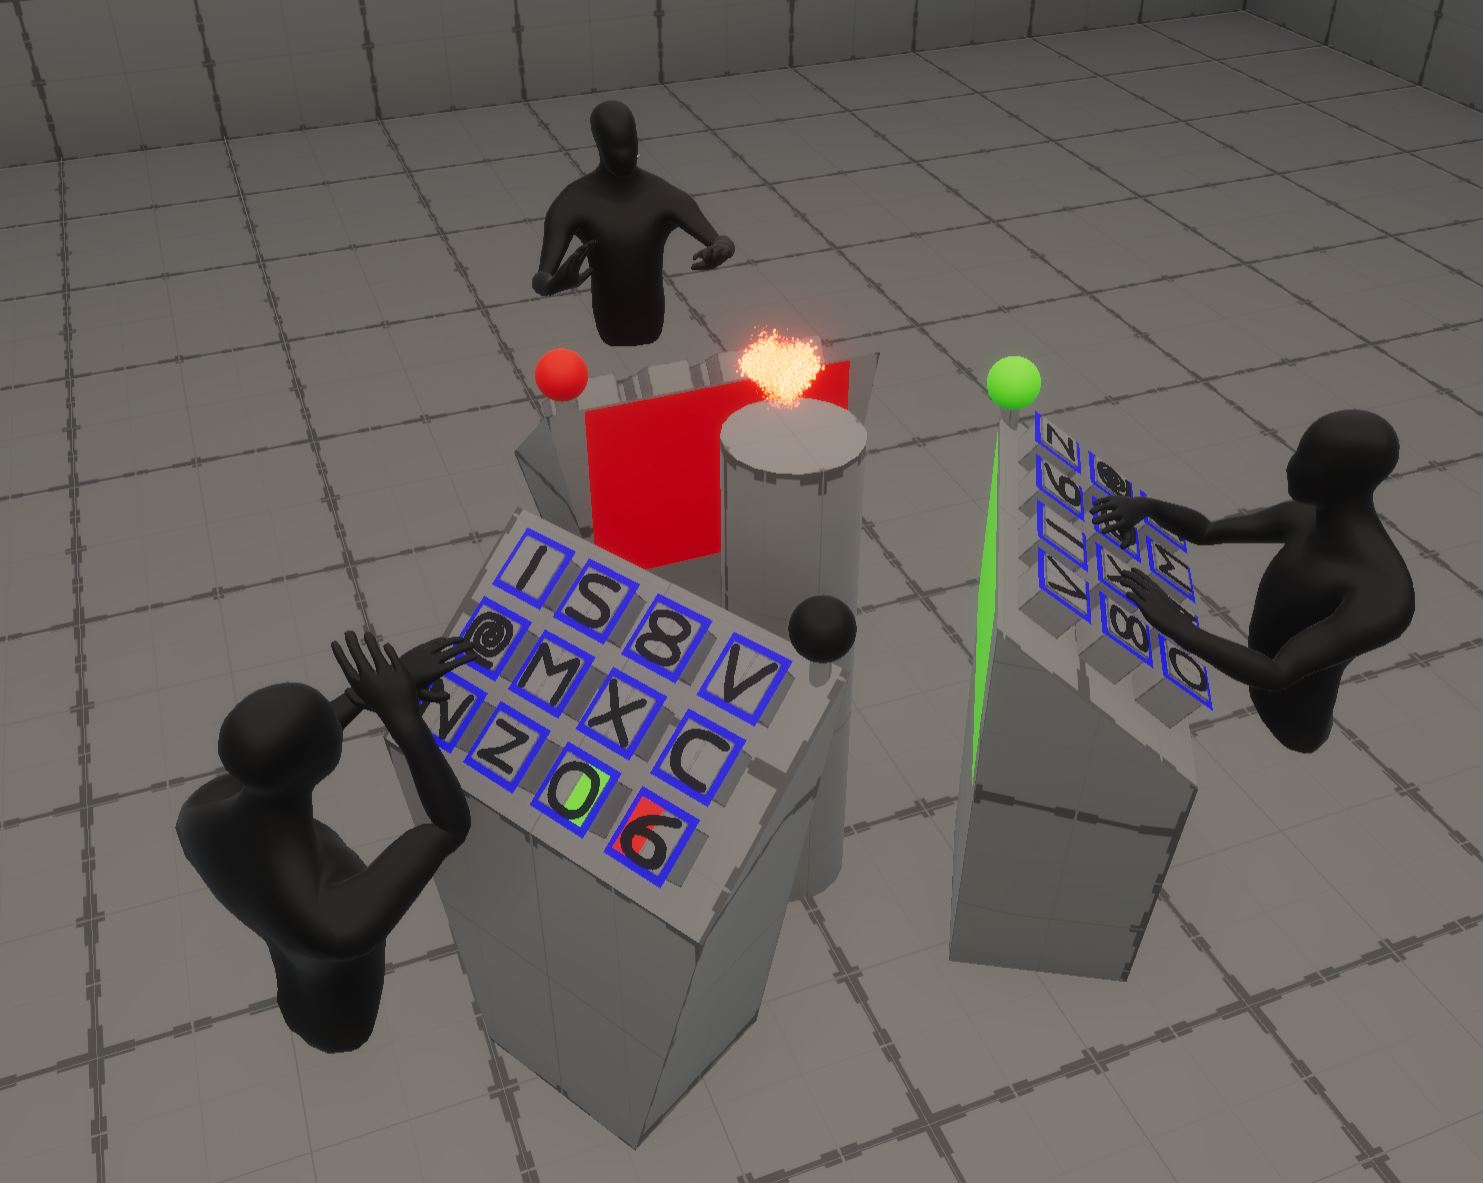
\includegraphics[width=0.4\linewidth]{Abbildungen/Podeste_IK_Avatars.jpg}}
  \qquad
  \subfloat[][]{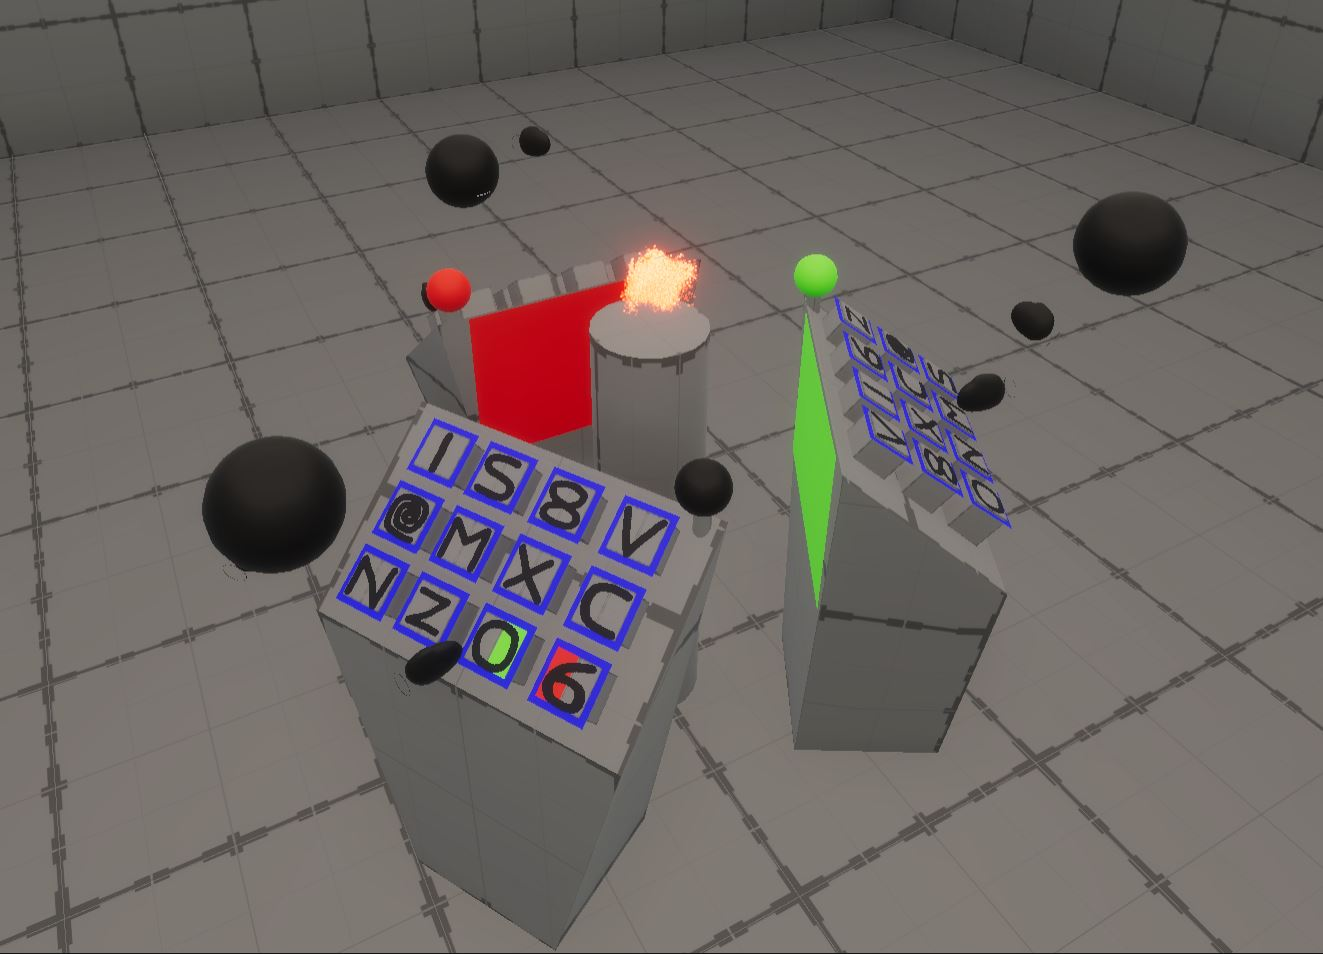
\includegraphics[width=0.442\linewidth]{Abbildungen/Podeste_Non_IK_Avatars.jpg}}
  \caption[Die Avatare und der Spectatorview]{Avatar-Konditionen \ac{ik} (a) und \ac{nik} (b) während der Versuchsdurchführung im Spectatorview.}
  \label{AvatareImEinsatz}
\end{figure}

\begin{figure}[H]
		\begin{footnotesize}
		\centering
			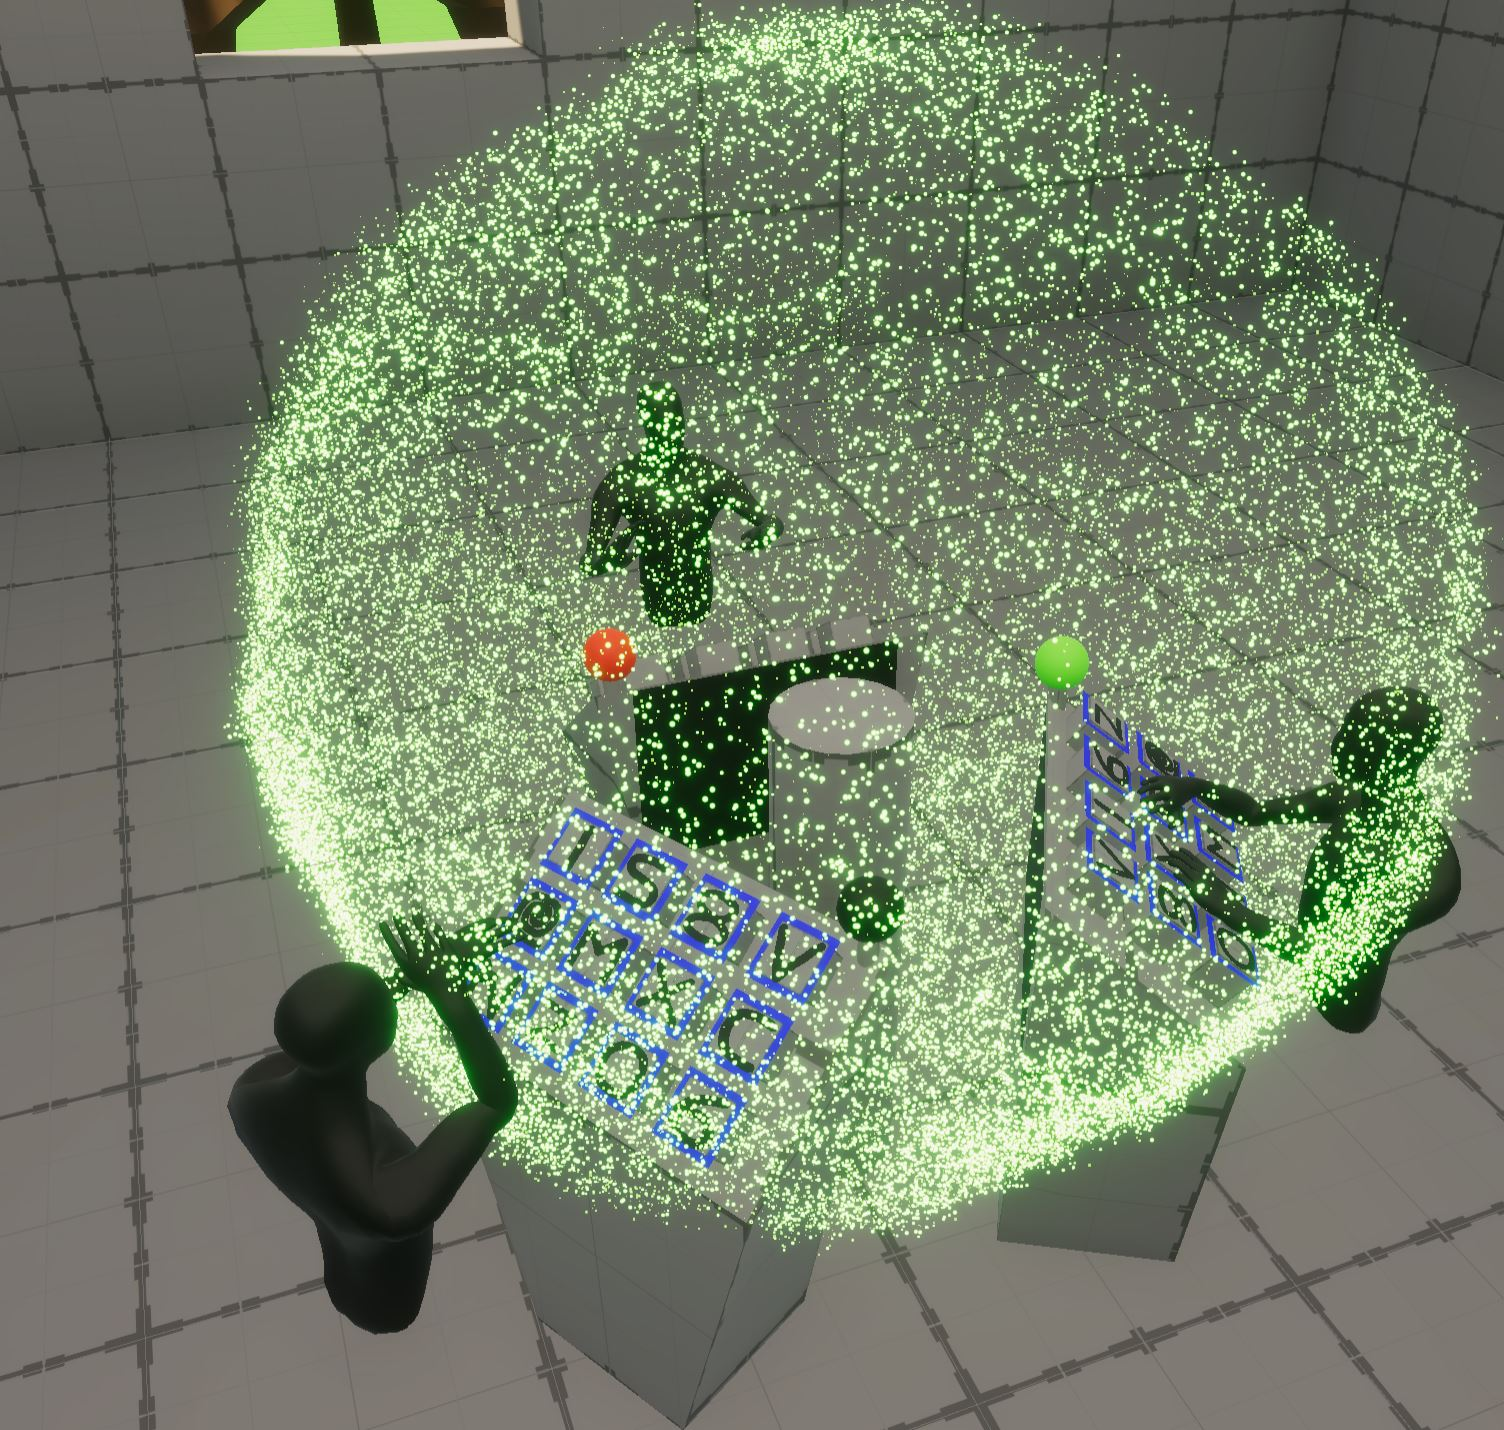
\includegraphics[scale=0.2]{Abbildungen/RoundSuccsessful.JPG}	
			\caption[Der Abschluss einer Runde]{Die Grüne Kugel erscheint bei einer erfolgreich abgeschlossenen Runde gut sichtbar für alle Teilnehmer.}
			\label{RoundFinished}
		\end{footnotesize}
	\end{figure}
	
\paragraph{Erwarteter Vertrauensaufbau}
Der zu erwartende Vertrauensaufbau des erklärenden Spielers einer Runde bezieht sich darauf, dass er seinen Mitspielern vertraut, die Symbole zuverlässig und ohne größere Probleme zu erraten. Der zu erwartende Vertrauensaufbau der Mitspieler bezieht sich darauf, dass diese dem erklärenden Spieler zutrauen, die Symbole zuverlässig zu erklären.

Zum Messen des \textit{kognitiven Vertrauens} der einzelnen Individuen, wird in dieser Studie ein Teilauszug des \textit{Cognitive-Trust-Scale} \citep[S. 37]{mcallister1995affect} (siehe \textit{Anhang \ref{Post-Questionnaire - Kognitives Vertrauen}}) genutzt.

\paragraph{Erwartete Teameffektivität}
Je mehr \textit{kognitives Vertrauen} sich durch die einzelnen Runden aufbaut, desto leichter fällt es den Teilnehmern, eine größere Anzahl an Runden abzuschließen. Und je weniger \textit{kognitives Vertrauen} sich durch die einzelnen Runden aufbaut, desto schwerer fällt es den Teilnehmern, eine größere Anzahl an Runden abzuschließen. Dies wird in Bezug zu den einzelnen Avatar-Konditionen betrachtet.

Zum Messen der \textit{wahrgenommenen Teameffektivität} der einzelnen Teilnehmer wird in dieser Studie ein Teilauszug des \textit{Team-Effectiveness-Scale} (siehe \textit{Anhang \ref{Post-Questionnaire - Team-Effektivität}}) \citep[S. 469]{gibson2003team} genutzt. Zum Messen der \textit{subjektiv wahrgenommenen Arbeitsbelastung} wird der NASA-TLX (siehe \textit{Anhang \ref{Post-Questionnaire - NASA-TLX}}) \citep{NASATLX} verwendet.
Zum Messen der \textit{Teameffektivität} wird die Anzahl der abgeschlossenen Runden des durchgeführten Experiments genutzt. Schafft ein Team eine Runde, hat dieses eine \textit{Teameffektivität} von 1, schafft es 10 Runden, hat es eine \textit{Teameffektivität} von 10.

\newpage
\subsection{Die Versuchsumgebung}
\label{TechnischeAnforderungen}
Das System besitzt folgende \textbf{technische Anforderungen}, die umgesetzt werden müssen:
\begin{itemize}
\item \textbf{Onlinefähigkeit und Unterstützung mehrerer \ac{hmd}s}: Da die Teilnehmer auch von zu Hause an dem Versuch teilnehmen können sollen, muss die gesamte Anwendung mehrere \ac{hmd}s unterstützen sowie auf sehr vielen verschiedenen Computermodellen zum Einsatz kommen können. Die gesamte Anwendung muss onlinefähig sein. Alle relevanten Statuszustände (Runde, Bewegungen und Positionen der Avatare, Rundenzeit, Status des jeweiligen Zustands des Podests eines Spielers etc.) müssen synchronisiert sein.
\item \textbf{Geringe Latenz}: Das gesamte System muss latenzfrei sein, um die Bewegungen und Interaktionen der Avatare für die Nutzer nachvollziehbar und realistisch zu machen.
\item \textbf{Steuerung und Verwaltung der Anwendung durch einen Spectator}: Damit der Versuchsleiter so wenig wie möglich in den Versuch eingreift, muss die Anwendung von außen über einen eigenen Spectator-Client gesteuert werden können.
\item \textbf{Interaktionsmöglichkeiten}: Es muss eine Übertragung der aktuellen Zustände der Knöpfe auf den Podesten zu allen Teilnehmern im \ac{sve} stattfinden.
\item \textbf{Sprachübertragung}: Es muss eine Sprachübertragung von einem Client zu allen Nutzern und von allen Nutzern zum Client stattfinden können.
\item \textbf{Avatar-Konditionen}: Es müssen die beiden Avatar-Konditionen \ac{ik} sowie\newline \ac{nik} im System vorhanden sein.
\end{itemize}

Weiterhin besitzt das System noch \textbf{zusätzliche Anforderungen} :

\begin{itemize}
\item \textbf{Teamfähigkeit} Das Team muss eine Aufgabe gemeinsam lösen. Jedes Teammitglied muss zu gleichen Teilen involviert sein. Fehlt ein Teammitglied, soll die Aufgabe nicht lösbar sein.
\item \textbf{Inkrementelle Erhöhung der Schwierigkeit} Um einen Vergleich zwischen der \textit{Teameffektivität} der unterschiedlichen Gruppen herzustellen, mussten die Runden inkrementell schwieriger werden. Dies wurde dadurch gelöst, dass die Teilnehmer nach jeder dritten Runde ein Symbol mehr gestikulieren oder erraten mussten.
%\item \textbf{Neutrale Avatare} Die Avatare sollen so neutral wie möglich gestaltet sein. 
\item \textbf{Vermeidung von Bekanntheit} Um die gegenseitige Bekanntheit der Teilnehmer auszuschließen, wurde jedem Teilnehmer zu Beginn des Versuchs ein zufälliger Name zugeordnet. Vor dem gesamten Versuch konnten sich die Teilnehmer nicht sehen oder hören.
Dadurch wird verhindert, dass die Teilnehmer bereits vor dem Versuch ein \textit{kognitives Vertrauen} oder \textit{kognitives Misstrauen} zu den anderen Personen aufbauen.
\item \textbf{Keine verbale Kommunikation} Da die Stimme der Teilnehmer ein Residuum ist, wurde die verbale Kommunikation von Versuchsteilnehmer zu Versuchsteilnehmer nicht gestattet. 
\end{itemize}

\subsubsection{Technik der Versuchsumgebung}
Um den Versuch durchzuführen, wurde ein \ac{sve} entwickelt, in dem sich die drei Teammitglieder gegenseitig als Avatare sehen und miteinander interagieren können. Das \ac{sve} ist mit Unity 2019.4.3f1 und der HD-Render-Pipeline entwickelt worden. Um die Echtzeitkommunikation zwischen den einzelnen Clients zu gewährleisten, wurde das Multiplayer-Framework \textit{Normcore v2.0}\footnote{www.Normcore.io} genutzt.
Normcore unterstützt Network-Physics simulationen, automatische Realtime- Synchronisation, Voice-Chat, XR-Kompatibilität sowie persistente Multiplayer-Räume.	

\paragraph{Normcore Datastore / Sync Mechanismus}
Normcore besitzt das Konzept eines globalen Datenspeichers. Alle Zustände, egal ob die Position eines Spielers, einzelne bool, integer oder float Variablen, können in einem globalen Datenspeicher gespeichert werden. Werden Objekte in der Anwendung bewegt, synchronisiert Normcore diese Änderung der Position und/oder Rotation automatisch bei allen anderen Mitspielern.

\paragraph{Auswahl der Hardware}
Um an dem Experiment teilnehmen zu können, benötigen die Teilnehmer ein in vollem Umfang funktionierendes SteamVR, Windows-Mixed-Reality oder ein Oculus Rift/Rift-S \ac{hmd} mit kompatiblen Controllern sowie einen leistungsstarken \ac{vr}-fähigen PC. Der Spectator, der das Experiment von außerhalb steuert und verwaltet, nutzt einen PC, auf dem die Anwendung ohne \ac{hmd} ausführbar ist.

\paragraph{VR-Client}
Jeder Versuchsteilnehmer benötigt eine Client Version der Anwendung, um an dem Versuch teilzunehmen. Die Client Version gibt es in drei verschiedenen Versionen. Diese verschiedenen Versionen unterstützen die SteamVR \ac{hmd}s, die Oculus Rift \ac{hmd}s und die Windows Mixed-Reality \ac{hmd}s. Beim Start des Clients gelangt der Teilnehmer in das \ac{sve} und verbindet sich automatisch mit dem Server (Normcore-Raum).

\paragraph{Spectator}
Der Spectator besitzt einen eigenen Client ohne eigene Repräsentation des Körpers und benötigt daher auch kein \ac{hmd}, um an der Session teilzunehmen. Dem Spectator ist es möglich, sich frei mit der Kamera in der Umgebung zu bewegen.
Er hat die Fähigkeit, das Spiel zu starten, die Nummer der zu beginnenden Runde einzustellen, einen Restart durchzuführen, sich die verbundenen Spieler anzuzeigen und herauszuwerfen, die Avatar-Kondition der Clients zwischen \ac{ik} und \ac{nik} zu wechseln sowie das Spiel zu verlassen.
Der Spectator kann beispielsweise Spieler herauszuwerfen, um die Session aufzuräumen und diese für das nächste Team vorzubereiten. Weiterhin besitzt der Spectator noch einige Funktionen, um Informationen über das aktuelle Spielgeschehen zu erhalten. So bekommt er die vergangene Zeit, die aktuelle Rundenzahl, die Effizienz des Teams, die Information über die Korrektheit der gewählten Eingaben der Spieler und die Anzahl der zu erklärenden Symbole angezeigt. Die Anzahl der im Raum anwesenden Spieler werden ebenfalls aufgeführt. So sieht der Spectator \textit{Player 1} bis \textit{Player 3} bei einem vollständigen Team auf seinem Bildschirm. 

Der Spectator-Client wird in \textit{Abbildung \ref{SpectatorView}} dargestellt.

%\begin{figure}[H]
%		\begin{footnotesize}
%		\centering
%			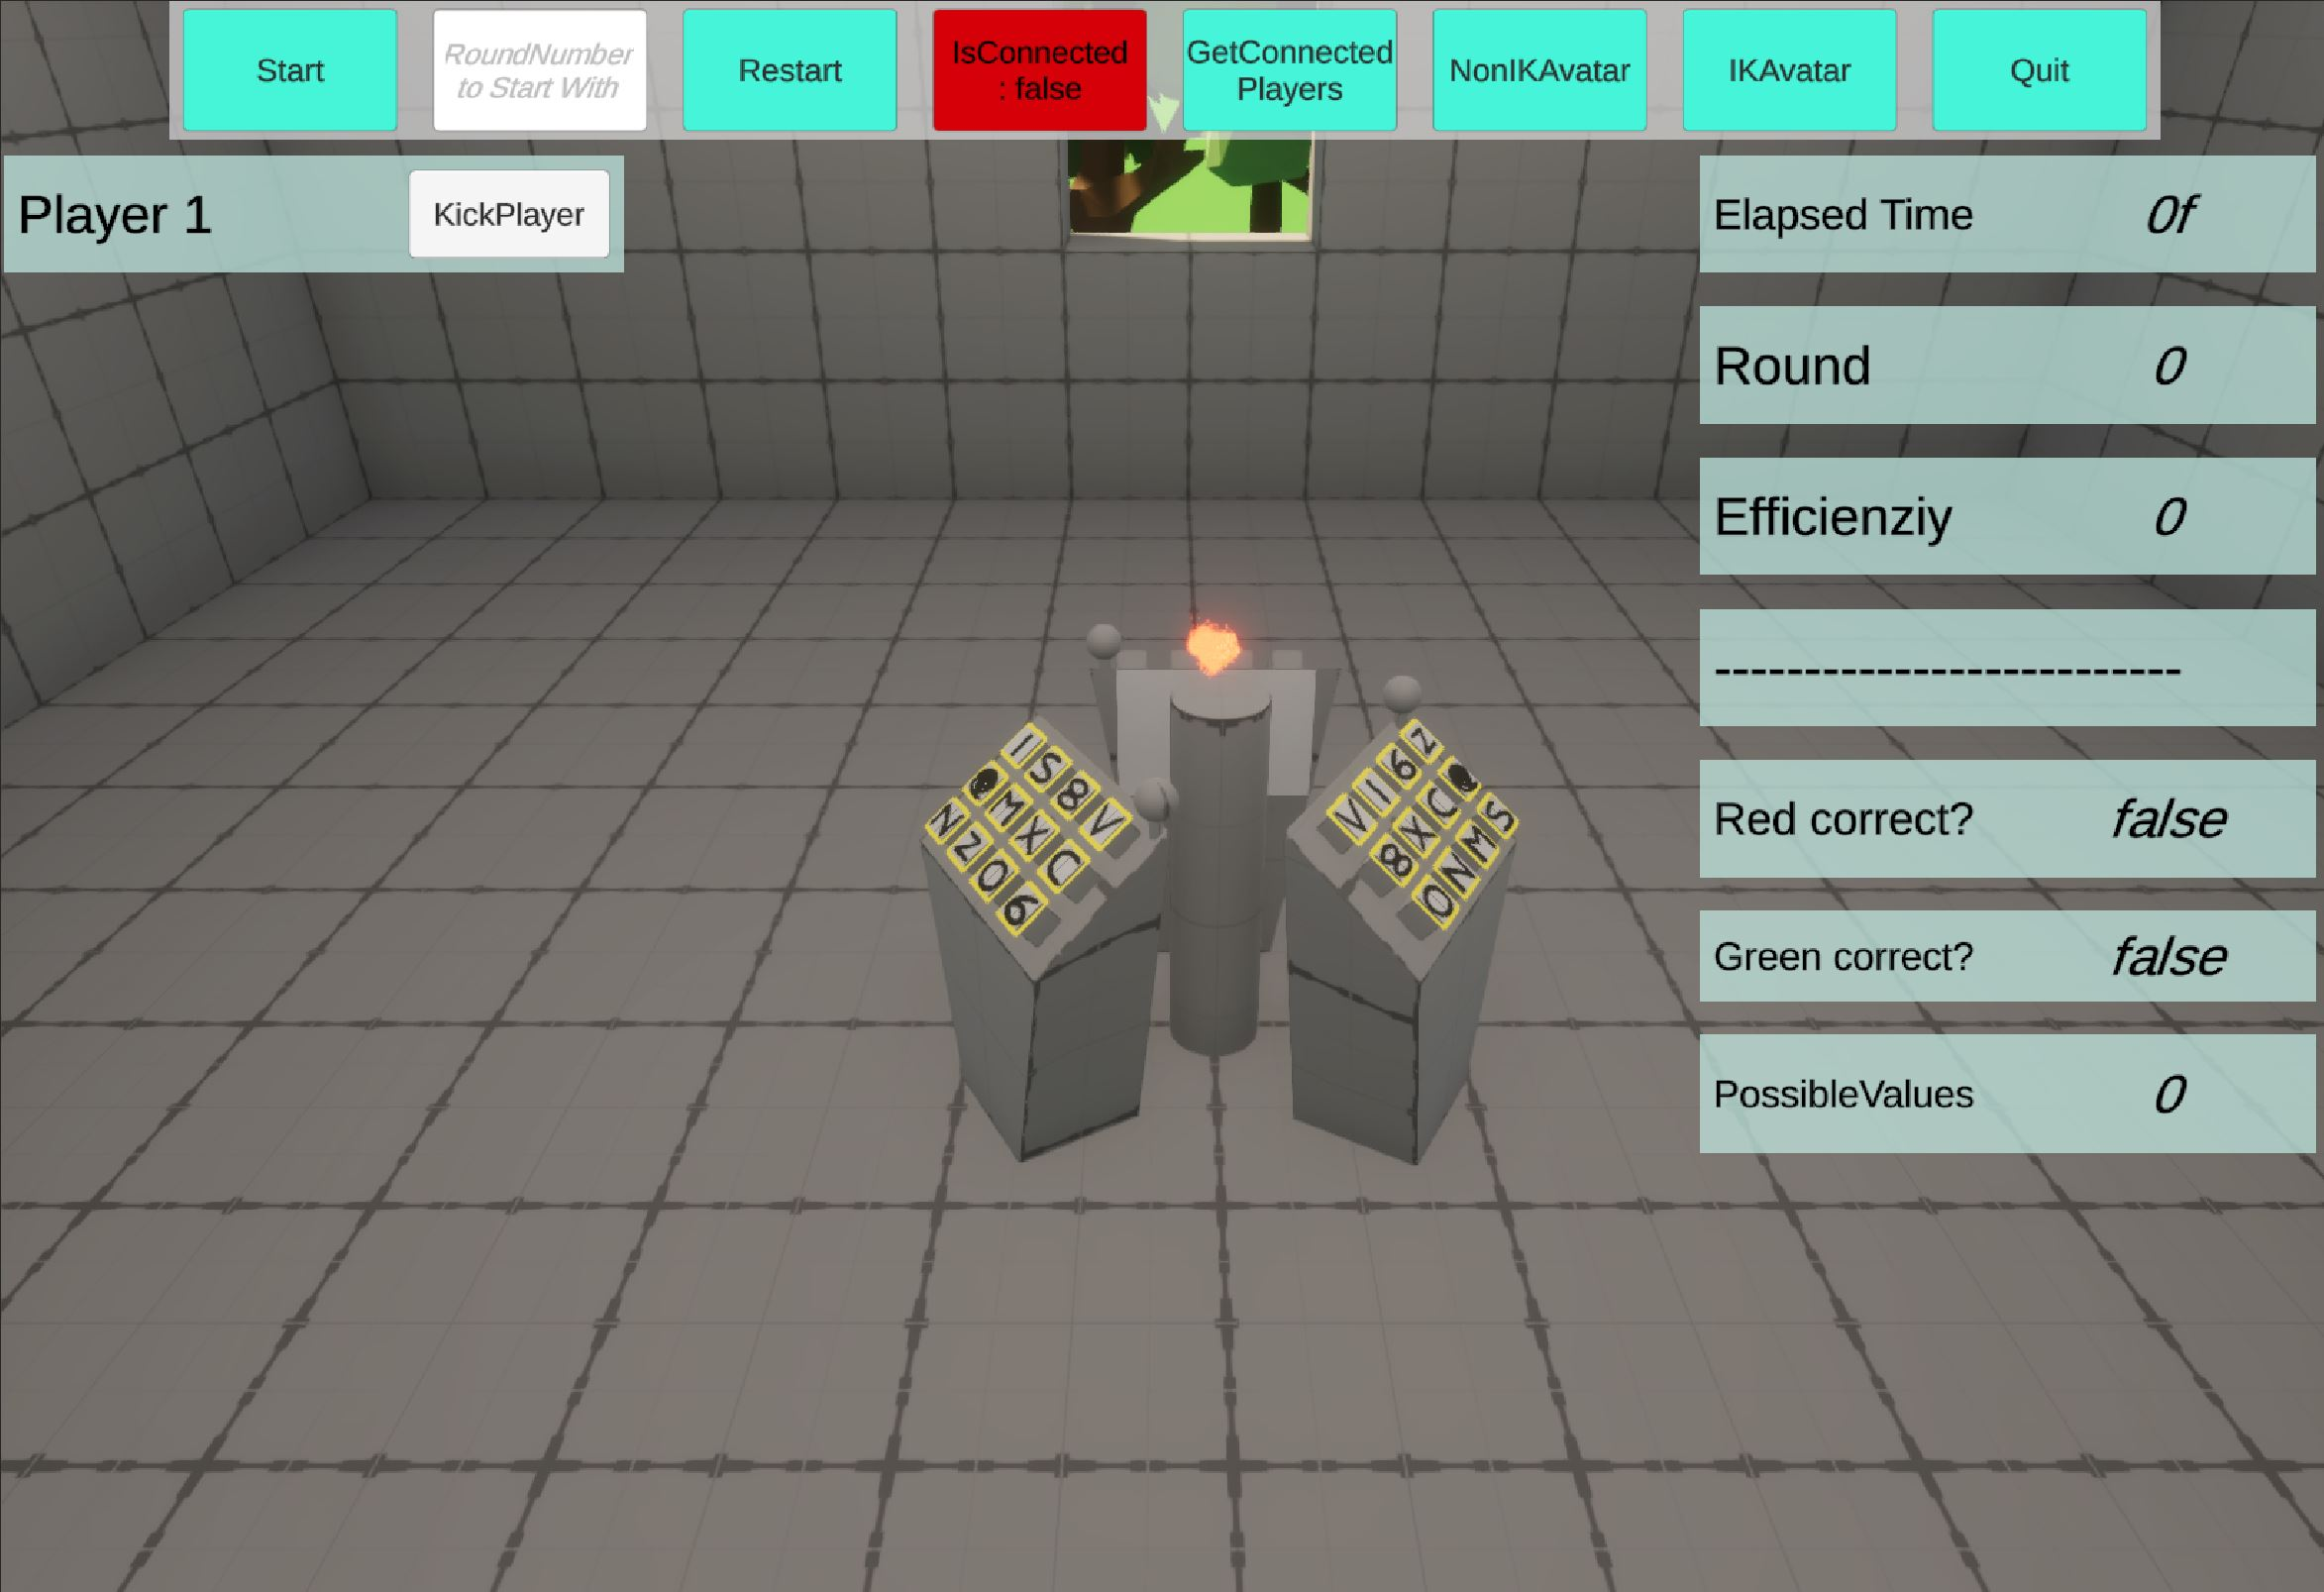
\includegraphics[scale=0.3]{Abbildungen/Versuchsumgebung/SpectatorView.JPG}
%			\caption[Der Spectatorview]{Diese Abbildung zeigt den Spectator-Client mit den verschiedenen Funktionen zum Verwalten des laufenden Versuchs.}
%			\label{SpectatorView}
%		\end{footnotesize}
%	\end{figure}
%
\begin{figure}[H]
  \centering
  \subfloat[][]{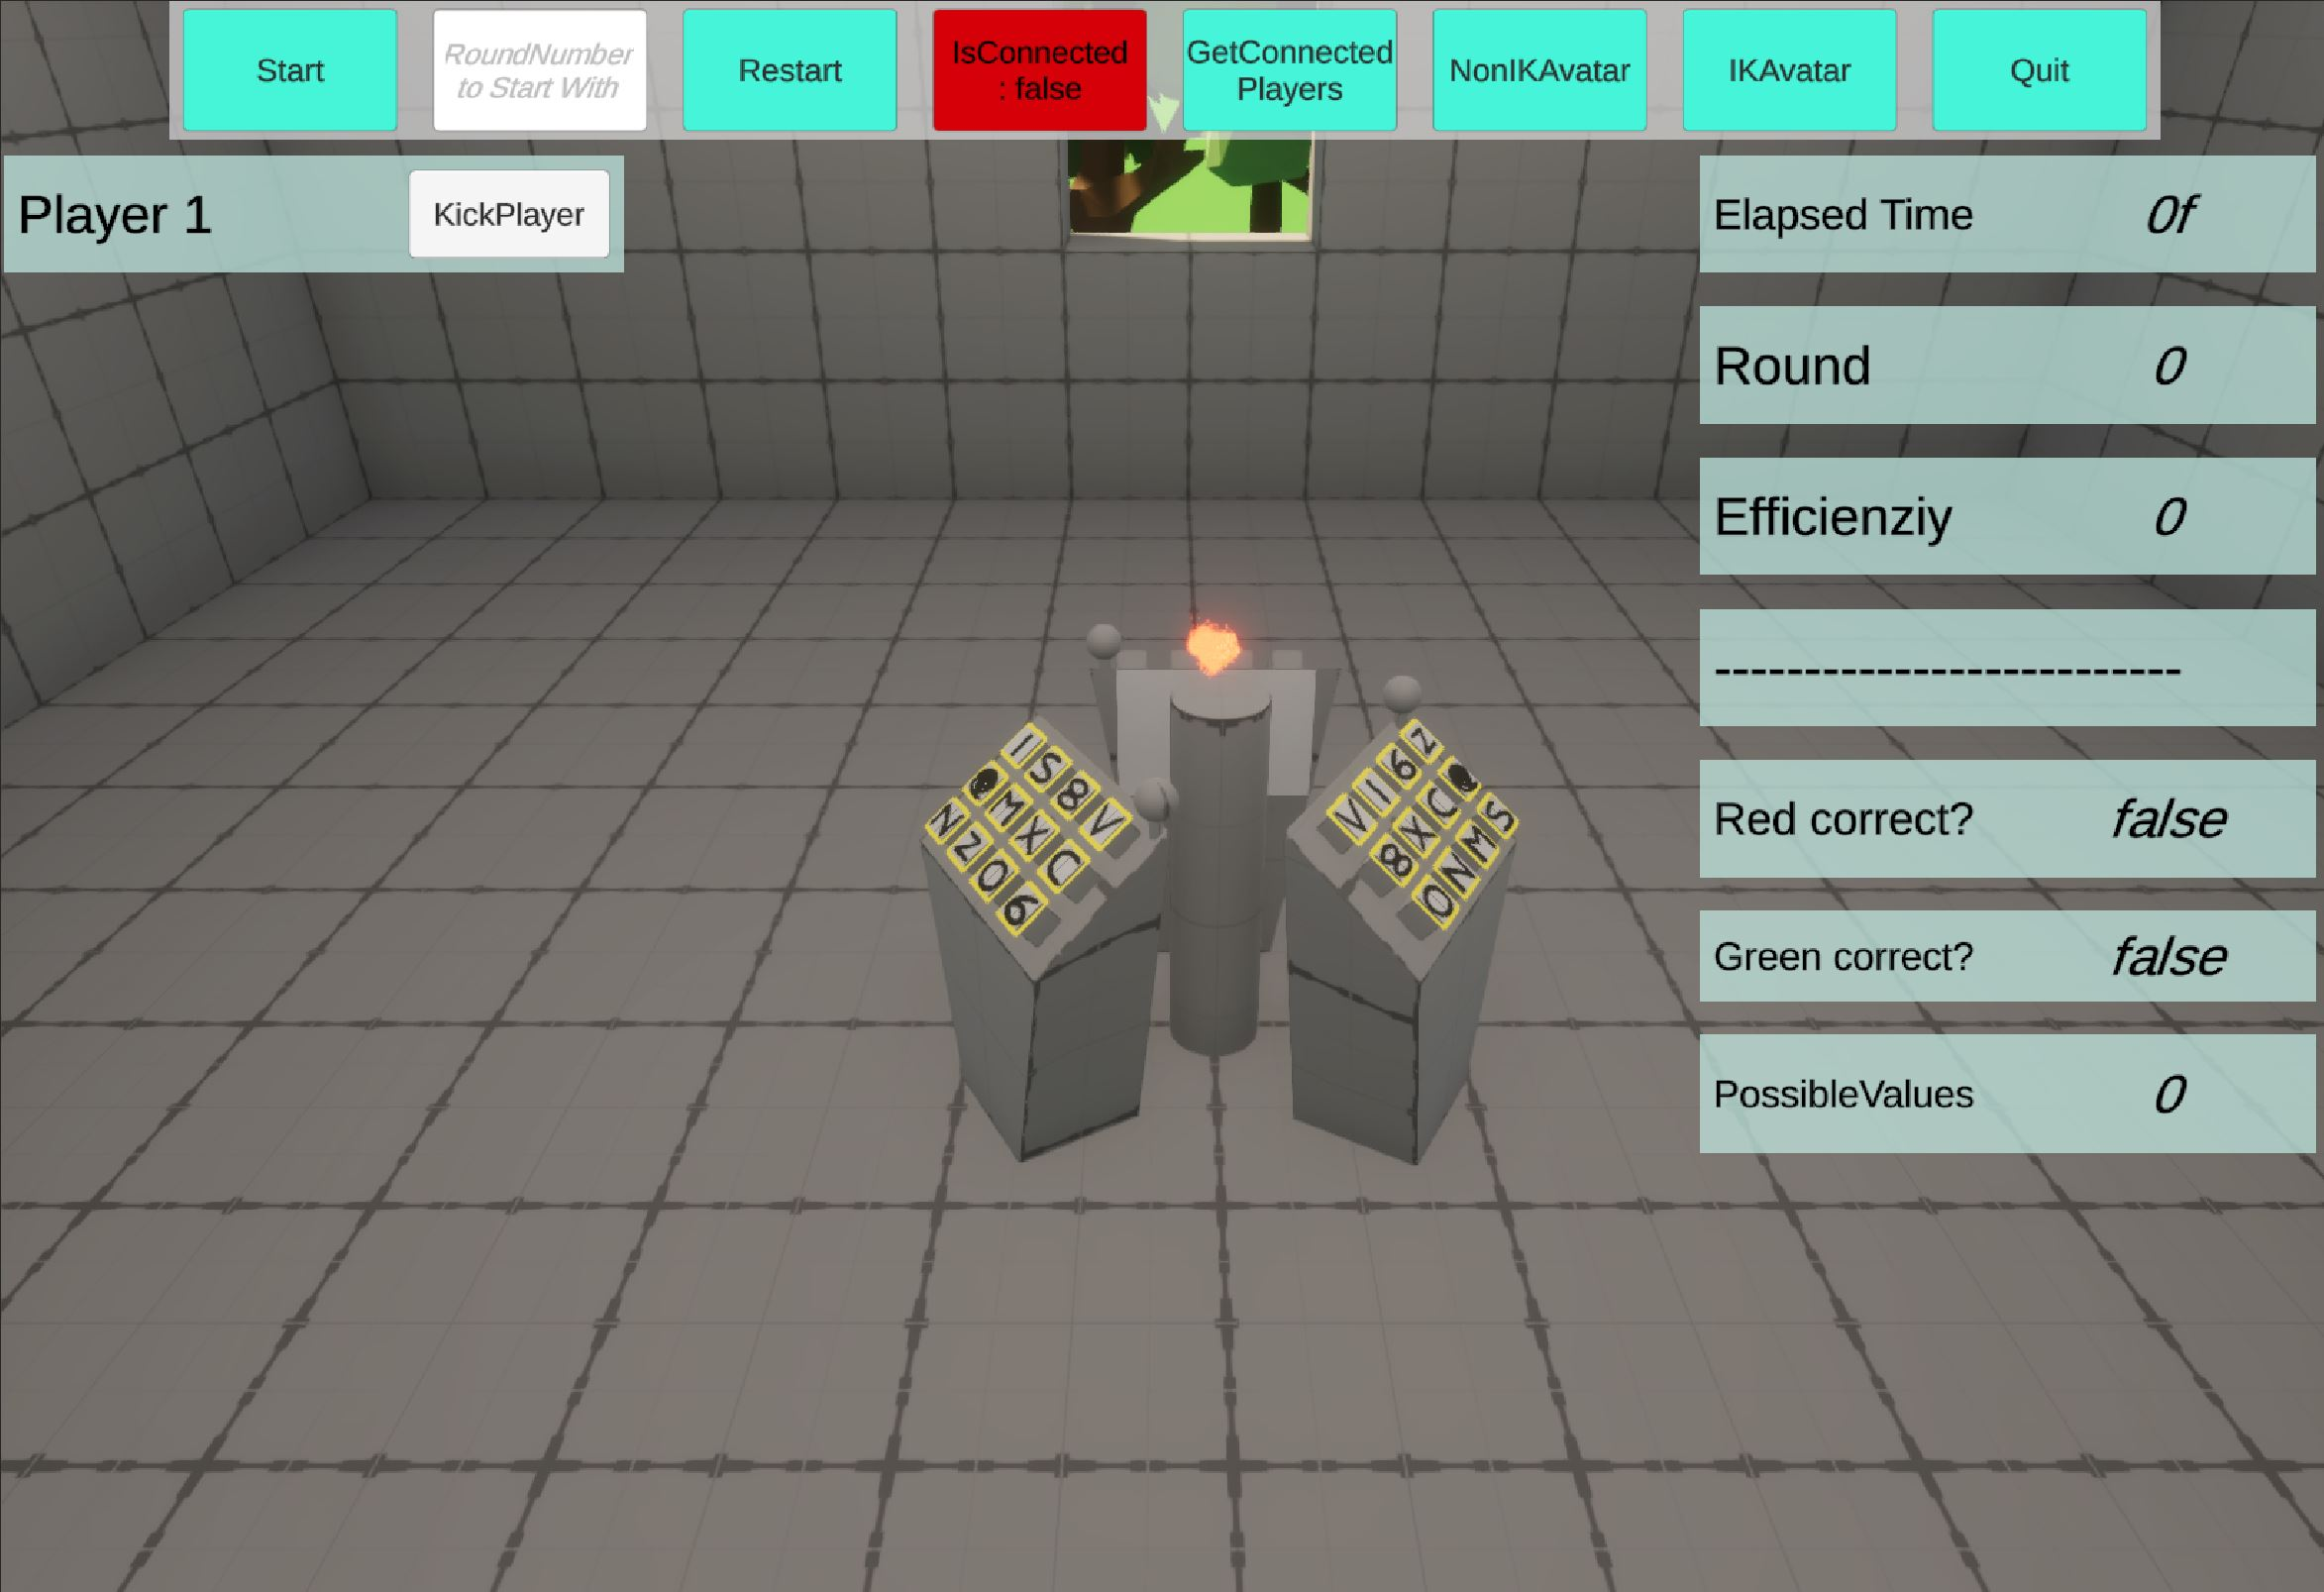
\includegraphics[width=0.7\linewidth]{Abbildungen/Versuchsumgebung/SpectatorView.JPG}}
  \qquad
  \subfloat[][]{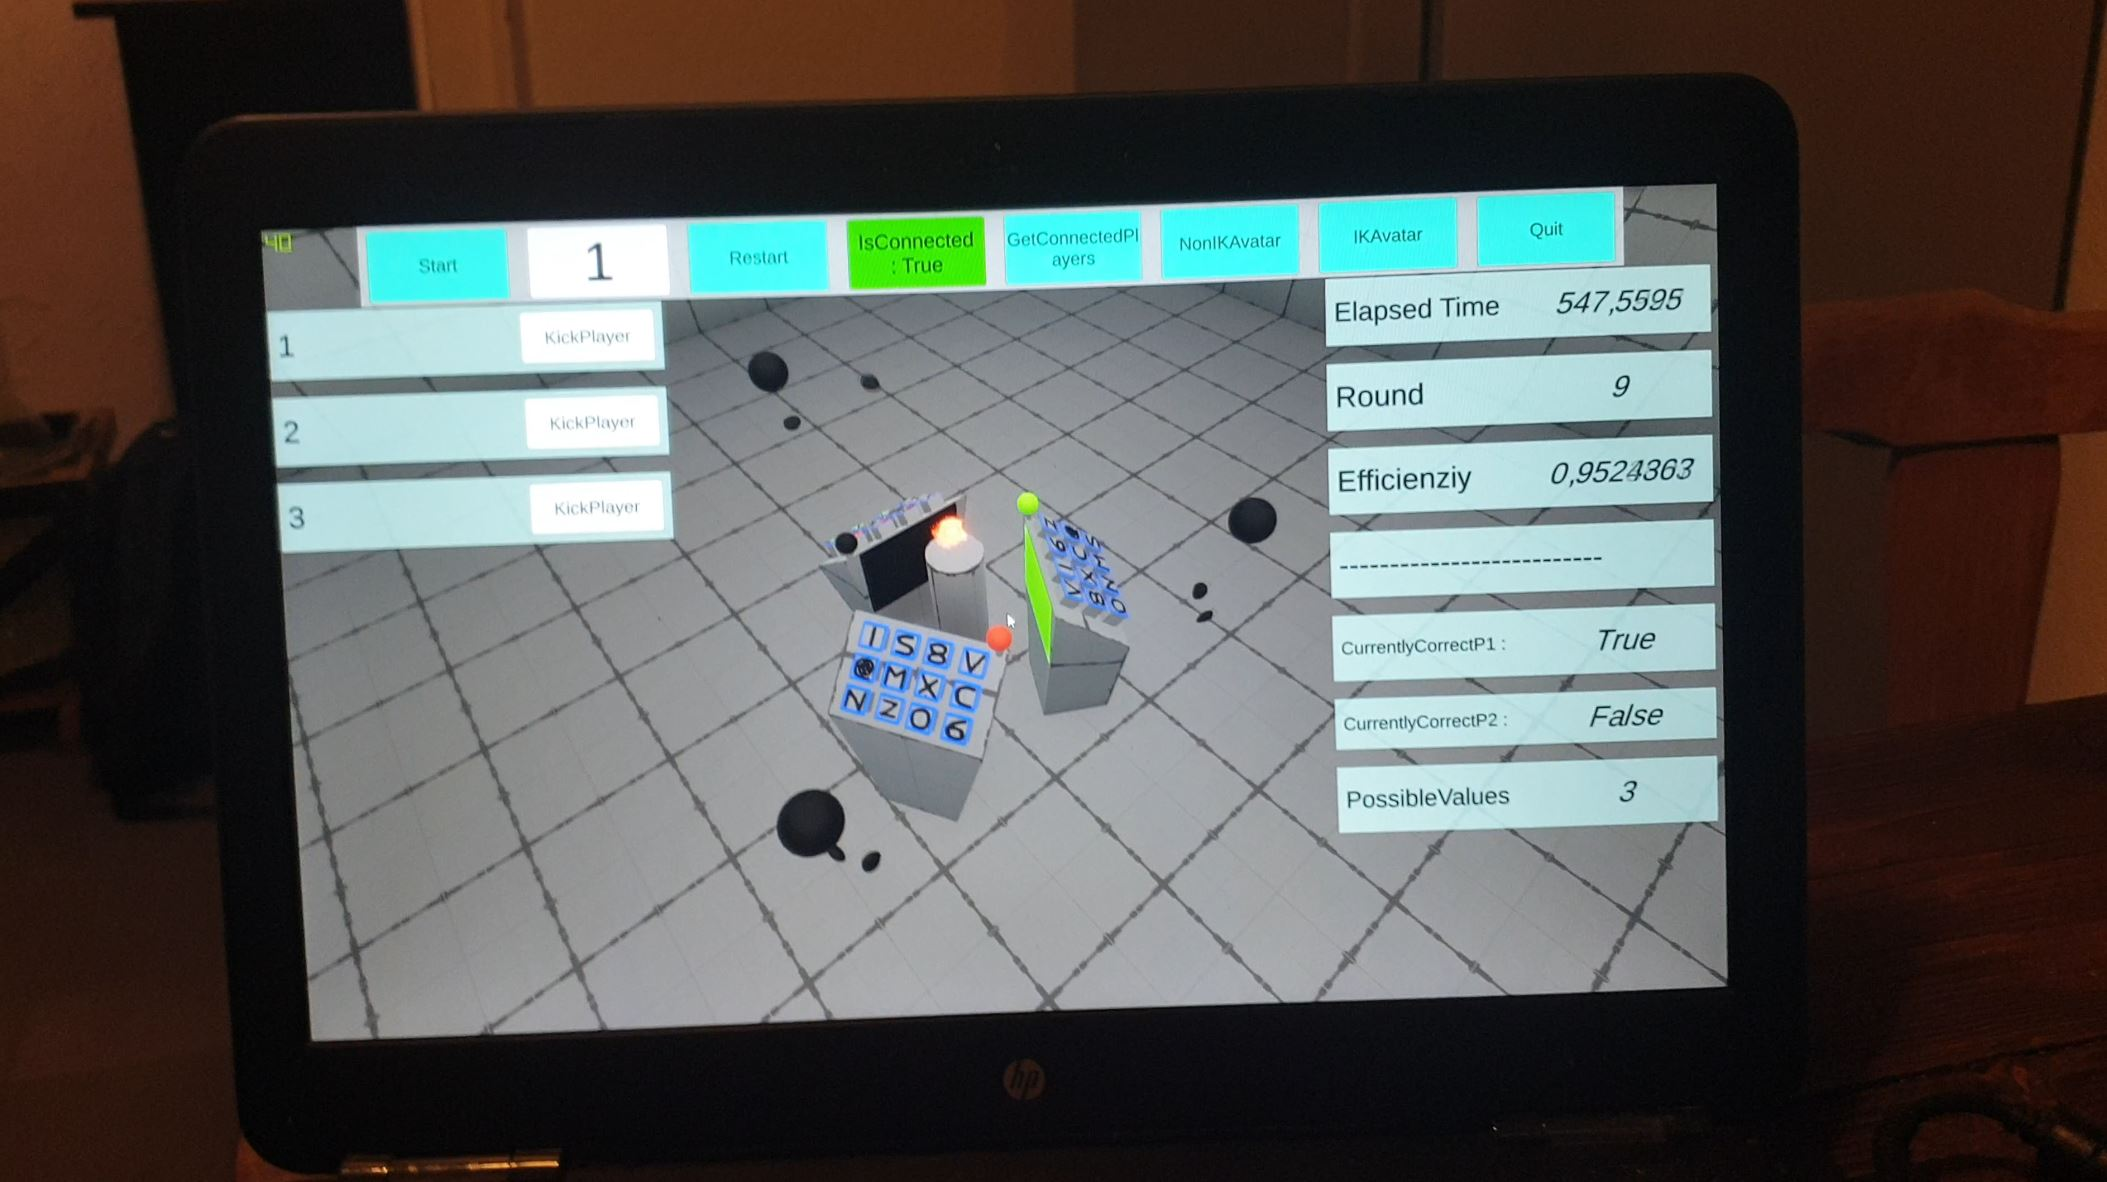
\includegraphics[width=0.7\linewidth]{Abbildungen/Versuchsumgebung/SpectatorView_OnLaptop.JPG}}
  \caption[Der Spectatorview]{Diese Abbildung zeigt den Spectator-Client mit den verschiedenen Funktionen zum Verwalten des laufenden Versuchs. (a) Ohne User und (b) während eines Versuchsdurchlaufes auf eines Laptop.}
  \label{SpectatorView}
\end{figure}

\paragraph{GameManager}
Der GameManager übernimmt alle wichtigen Funktionen zur Steuerung der Anwendung und der Netzwerkkommunikation.
Diese sind unter anderem:
\begin{itemize}[itemsep=0cm]
\item Steuerung und Entscheidungslogik der Runden
\item Netzwerkmanagement und RPC-Handling
\item Start, Reset, Überprüfungsmechanismen sowie Zeitmessungen der einzelnen Runden
\item Interaktionen und Verwaltung von globalen Datastore-Variablen
\end{itemize}

Die Netzwerkkommunikation zwischen den einzelnen Clients und dem Spectator wird vom \textit{GameManager} verwaltet. Der Spectator sowie der Client besitzen \textit{GameManager} mit unterschiedlichen Funktionalitäten. Der \textit{GameManager des Clients} übernimmt das für den Client relevante RPC-basierte Netzwerkhandling. Gleichzeitig lauscht dieser auf Änderungen von relevanten Variablen im globalen Datastore. Eine wesentliche Aufgabe ist es, zu überprüfen, ob eine Runde vom \textit{GameManager des Spectators} als beendet markiert wurde um gegebenenfalls die Initialisierung einer neuen Runde einzuleiten.

Der \textit{GameManager des Spectators} gibt hauptsächlich Information über den Start, Stop oder den Reset der einzelnen Runden an die \textit{GameManager} der Clienten weiter. Weiterhin steuert dieser aufgrund seiner besonderen Rolle ebenfalls die Spectator-to-Client Netzwerkinteraktionen, die Audioübertragung, den Kickmechanismus, die Rundenauswahl und das Aussehen der Avatare.
In \textit{Abbildung \ref{GameManagerClientSpectator}} wird ein grober Überblick über die Zusammenhänge und Funktionalitäten der \textit{GameManager} untereinander gegeben.

Die \textit{GameManager der Clients} stehen in Verbindung mit den einzelnen Podesten der Spieler. Der PodestManager eines jeweiligen Clients verwaltet die Podeste, welche wiederum einzelne Knöpfe eines Podests verwalten. 
Drückt ein Spieler einen Knopf, um ein Symbol ein- oder auszuloggen, sendet der Knopf eine Information über seinen Zustand an den Podestmanager des Clients. Dieser überprüft wiederum, ob die in diesem Moment gedrückten Knöpfe mit dem Auftrag der Runde übereinstimmen. Falls die gedrückten Knöpfe mit den zu drückenden Knöpfen dieser Runde übereinstimmen, wird eine boolean-Variable in einem globalen Datastore umgeschaltet, die den \textit{GameManager} des Spectators darüber informiert, dass ein Teilnehmer die korrekten Knöpfe dieser Runde gedrückt hat. Haben der rote und grüne Spieler die korrekten Knöpfe gedrückt und dadurch eine Flag im globalen Datastore über die jeweilige Korrektheit gesetzt, registriert der \textit{GameManager} des Spectators dies und setzt einen Flag über das erfolgreiche Abschließen der Runde. Die Clients registrieren dies und leiten die Startsequenz der nächsten Runde ein. 

\begin{figure}[H]
		\begin{footnotesize}
		\centering
			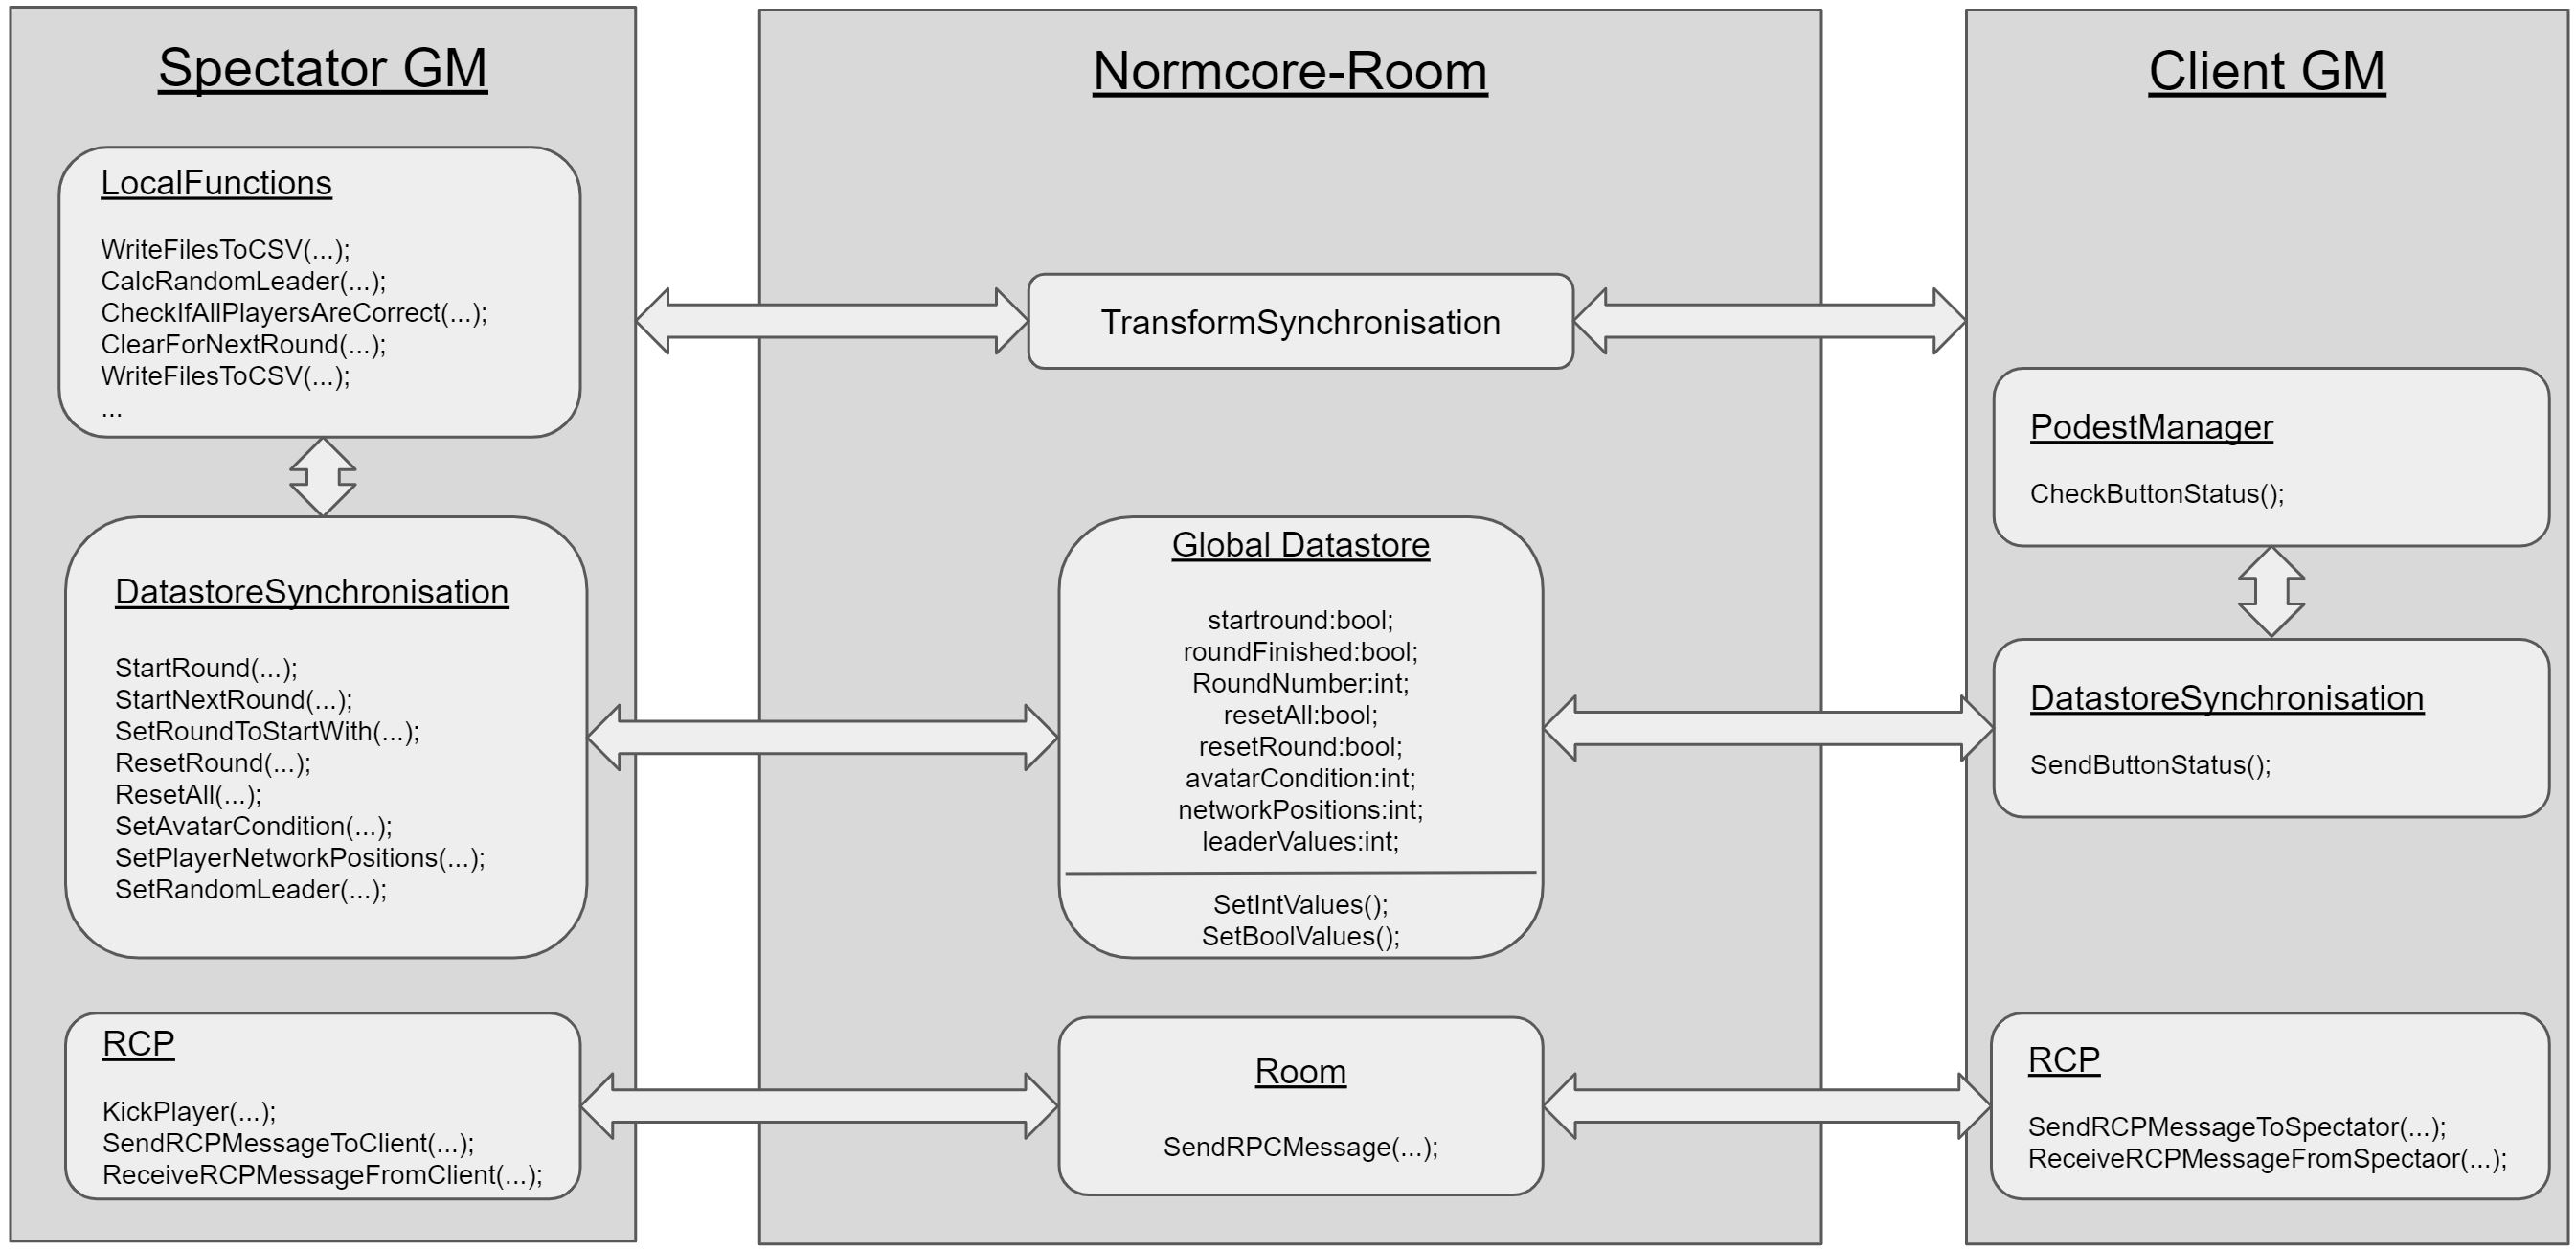
\includegraphics[width=\textwidth]{Abbildungen/GameManagerClientSpectator.jpg}
			\caption[Funktionalitäten des GameManagers]{Diese Abbildung gibt einen groben Überblick über die Zusammenhänge der Funktionalitäten der GameManager des Experiments im \ac{sve} .}
			\label{GameManagerClientSpectator}
		\end{footnotesize}
	\end{figure}

\paragraph{Audioübertragung}
Die Audioübertragung wird vom GameManager des Clients sowie dem Spectator verwaltet. Sobald ein Teilnehmer mit dem Normcore-Netzwerk verbunden ist, wird das Mikrofon des \ac{hmd}s aktiviert. Es werden unterschiedliche MessageID’s für Spectator und Client für die Netzwerkpakete festgelegt. Die serialisierten Audiodaten werden mittels RCP-Message an alle verbundenen Teilnehmer gesendet. Der Spectator liest nur die Netzwerknachrichten mit der MessageID der Clients und der Client liest die Netzwerknachrichten mit der MessageID des Spectators.

\textit{Abbildung \ref{ClientRCPMessageReceived}} zeigt den Programmcode des Spectator für das Eingehen einer RCP-Nachricht beispielhaft. Wird ein RCP-Paket erkannt, wird dieses entpackt und die MessageID in den ersten 32-Bits der RCP-Message ausgelesen. Je nach MessageID, dient das RCP-Paket einem anderen Zweck. Da der Spectator nur Audiostreams des Clients empfängt, muss dieser RCP-Messages mit einer MessageID von \glqq{}2000\dq{} verarbeiten. 
Wird die RCP-Message entpackt und es befindet sich die MessageID für Audiostreams vom Client in der Nachricht, wird dieser vom \glqq{}NetworkAudioReceiver\dq{} des Spectators verarbeitet. Falls kein \glqq{}NetworkAudioReceiver\dq{} vorhanden ist, wird ein neuer erstellt. Loggt sich ein neuer Client in das \ac{sve} ein und sendet einen Audiostream, wird für diesen Client ein neuer \glqq{}NetworkAudioReceiver\dq{} erstellt.

\begin{figure}[H]
		\begin{footnotesize}
		\centering
			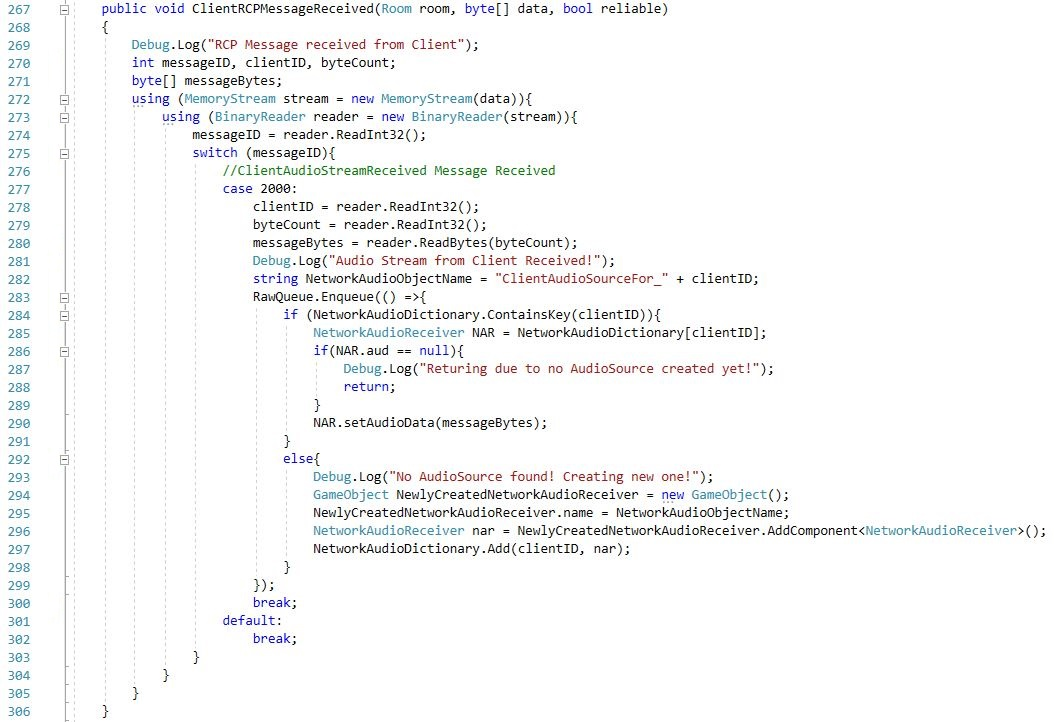
\includegraphics[width=\textwidth]{Abbildungen/ClientRCPMessageReceived.jpg}	
			\caption[RCP-Message Handling]{Programmcode zum Empfangen von Client RCP-Messages des Spectators.}
			\label{ClientRCPMessageReceived}
		\end{footnotesize}
	\end{figure}
	
\paragraph{Normcore Variable-Sync}
Um die Variablen im globalen Datenspeicher zu ändern, muss für jeden Datentyp eine Sync-Klasse geschrieben werden. Diese Sync-Klasse (siehe \textit{Abbildung \ref{boolSync}}) informiert den globalen Datenspeicher darüber, dass eine Variable geändert wurde. Der globale Datenspeicher informiert alle auf diese Variable zugreifenden Systeme darüber, dass eine Variable im globalen Datenspeicher geändert wurde und diese sich updaten sollen.

\begin{figure}[H]
		\begin{footnotesize}
			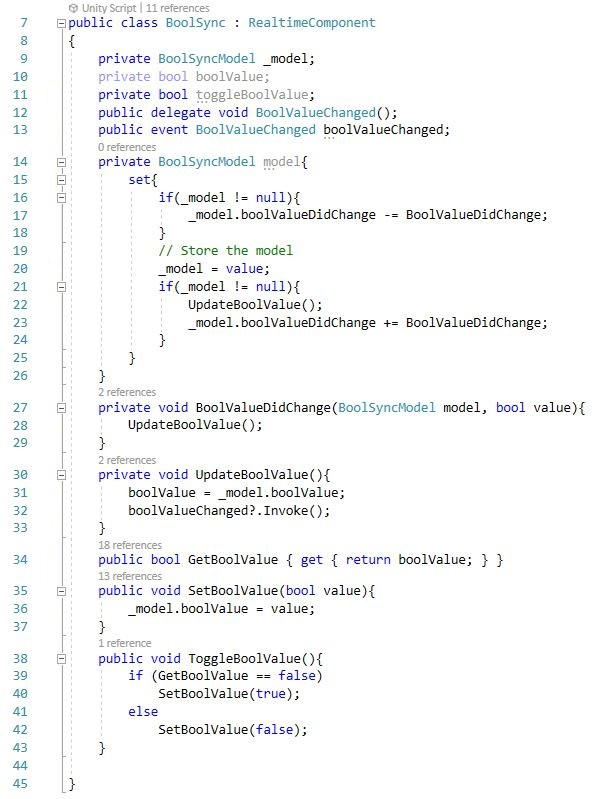
\includegraphics[scale=.75]{Abbildungen/boolValueChanged.jpg}
			\caption[Update von globalen Variablen]{Programmcode zum Update einer globalen Variable.}
			\label{boolSync}
		\end{footnotesize}
	\end{figure}

\paragraph{Rundenschwierigkeit}
Ein ScriptableObject beinhaltet die Regeln sowie den Ablauf der einzelnen Runden. Es ermöglicht einen Vergleich der Teams, da jedes Team jeweils in derselben Reihenfolge dieselben Zeichen angezeigt bekommt. Das ScriptableObject beinhaltet somit die allgemeinen Rundeneinstellungen des Spiels. In jeder Runde bestimmt es die Anzahl der zu erratenden Symbole, die Zuteilung der Symbole auf die Knöpfe der Podeste und die Farbzuteilung der Spieler. Die Regeln wurden so definiert, dass der erklärende Spieler spätestens nach jeder dritten Runde wieder mit dem Erklären an der Reihe ist. Zudem wird nach jeder dritten Runde die Anzahl der zu erratenden Symbole um eins erhöht. Somit muss beispielsweise in den Runden 1-3 ein Symbol und in den Runden 4-6 zwei Symbole erraten und erklärt werden. Wer in einer Runde der schwarze, grüne oder rote Spieler ist und welche Symbole gedrückt werden müssen, wurde einmalig in den RoundRules pseudozufällig festgelegt.

\textit{Abbildung \ref{RoundDifficulty}} zeigt die steigenden Schwierigkeitswerte, anhand derer in diesem Experiment die \textit{Teameffektivität} gemessen wurde.

\begin{figure}[H]
		\begin{footnotesize}
		\centering
			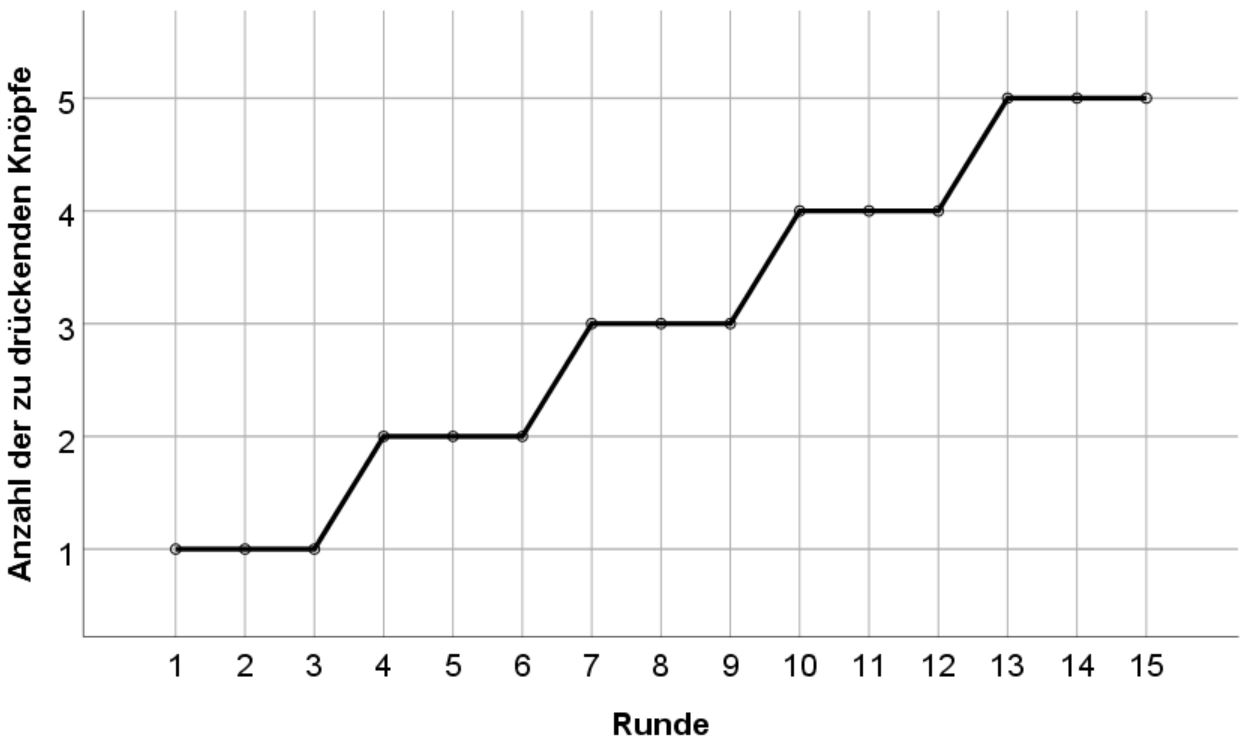
\includegraphics[scale=0.4]{Abbildungen/RoundDifficulty.JPG}	
			\caption[Der Schwierigkeitsgrad der Runden]{Die steigende Schwierigkeit der zu erratenden Symbole der einzelnen Runden. In Runde 1-3 muss ein Symbol erraten werden, in Runde 3-6 zwei Symbole usw.}
			\label{RoundDifficulty}
		\end{footnotesize}
	\end{figure}

\paragraph{CSV-Logwriting}
Der GameManager des Spectators sammelt alle relevanten Daten über die Clients, während die einzelnen Runden von den Teilnehmern durchgespielt werden. Es wird ein CSV-Log pro Durchgang inkrementell fortgeschrieben. Dieses Log umfasst unter anderem das Startdatum, die Startzeit, die Spielzeit, die Rundenzeit, die Rundennummer sowie die verwendete Avatar-Kondition.

\paragraph{Gametimer Funktionsweise}
Die jeweiligen Teams haben 600 Sekunden Zeit, um so viele Symbole wie möglich, richtig zu erkennen. Vor jeder Runde zählt ein Timer von 10 herunter, damit die Spieler kurz Zeit haben, sich auf die neue Runde einzustellen. Der Countdown ist für jeden Spieler zwischen den drei Podesten gut sichtbar platziert und wird jedem Spieler frontal angezeigt. Die 10 Sekunden zwischen den einzelnen Runden werden nicht zur Gesamtzeit hinzugezählt. Schaffen die Versuchsteilnehmer 10 Runden in 600 Sekunden zu absolvieren, dauert der Versuch somit insgesamt \\
$600 + 10 * 10 = 700$.

\paragraph{Sounds}
Tritt ein Teilnehmer dem Raum bei, wird der selbst aufgenommene Sound "Player
Connected“ abgespielt. Findet ein Disconnect statt, wird der Sound "Player
Disconnected“ abgespielt. Beim erfolgreichen Drücken eines Buttons ist ein Klick-Geräusch zu hören, um dem Spieler ein Feedback zu geben. 

\newpage	
%\paragraph{PlayerDisconnection Handling, Player Kick Mechanism, Destroying of Network Audio Receiver}	
	%\paragraph{Symbole und Podest, Drückmechanismus, Colliderplatzierung}
%Eingeloggt ist Gelb umrandet etc auch erklären, Ausloggen etc. Depth of button
\subsubsection{Optik der Versuchsumgebung}
\paragraph{Aussehen der Umgebung}
Die Teilnehmer befinden sich in einem rechteckigen Raum mit vier Fenstern, vor denen einige Low-Poly Bäume platziert sind. Durch die Fenster und die davor stehenden Bäume wird eine gewisse Offenheit erzeugt, damit die Teilnehmer sich nicht in dem \ac{sve} eingesperrt fühlen. Weiterhin wurde der Raum in einer schlichten gräulichen Farbe gehalten, um nicht von dem Spiel und den darin verwendeten Farben abzulenken. Die Spieler sollen sich dadurch bestmöglich auf den Versuch konzentrieren können. Die gesamte Umgebung ist zudem möglichst performant entwickelt worden, damit sie mit vielen Systemen eingesetzt werden kann. Die \textit{Abbildung \ref{Versuchsumgebung}} zeigt die Versuchsumgebung von außen.

\begin{figure}[H]
		\begin{footnotesize}
		\centering
			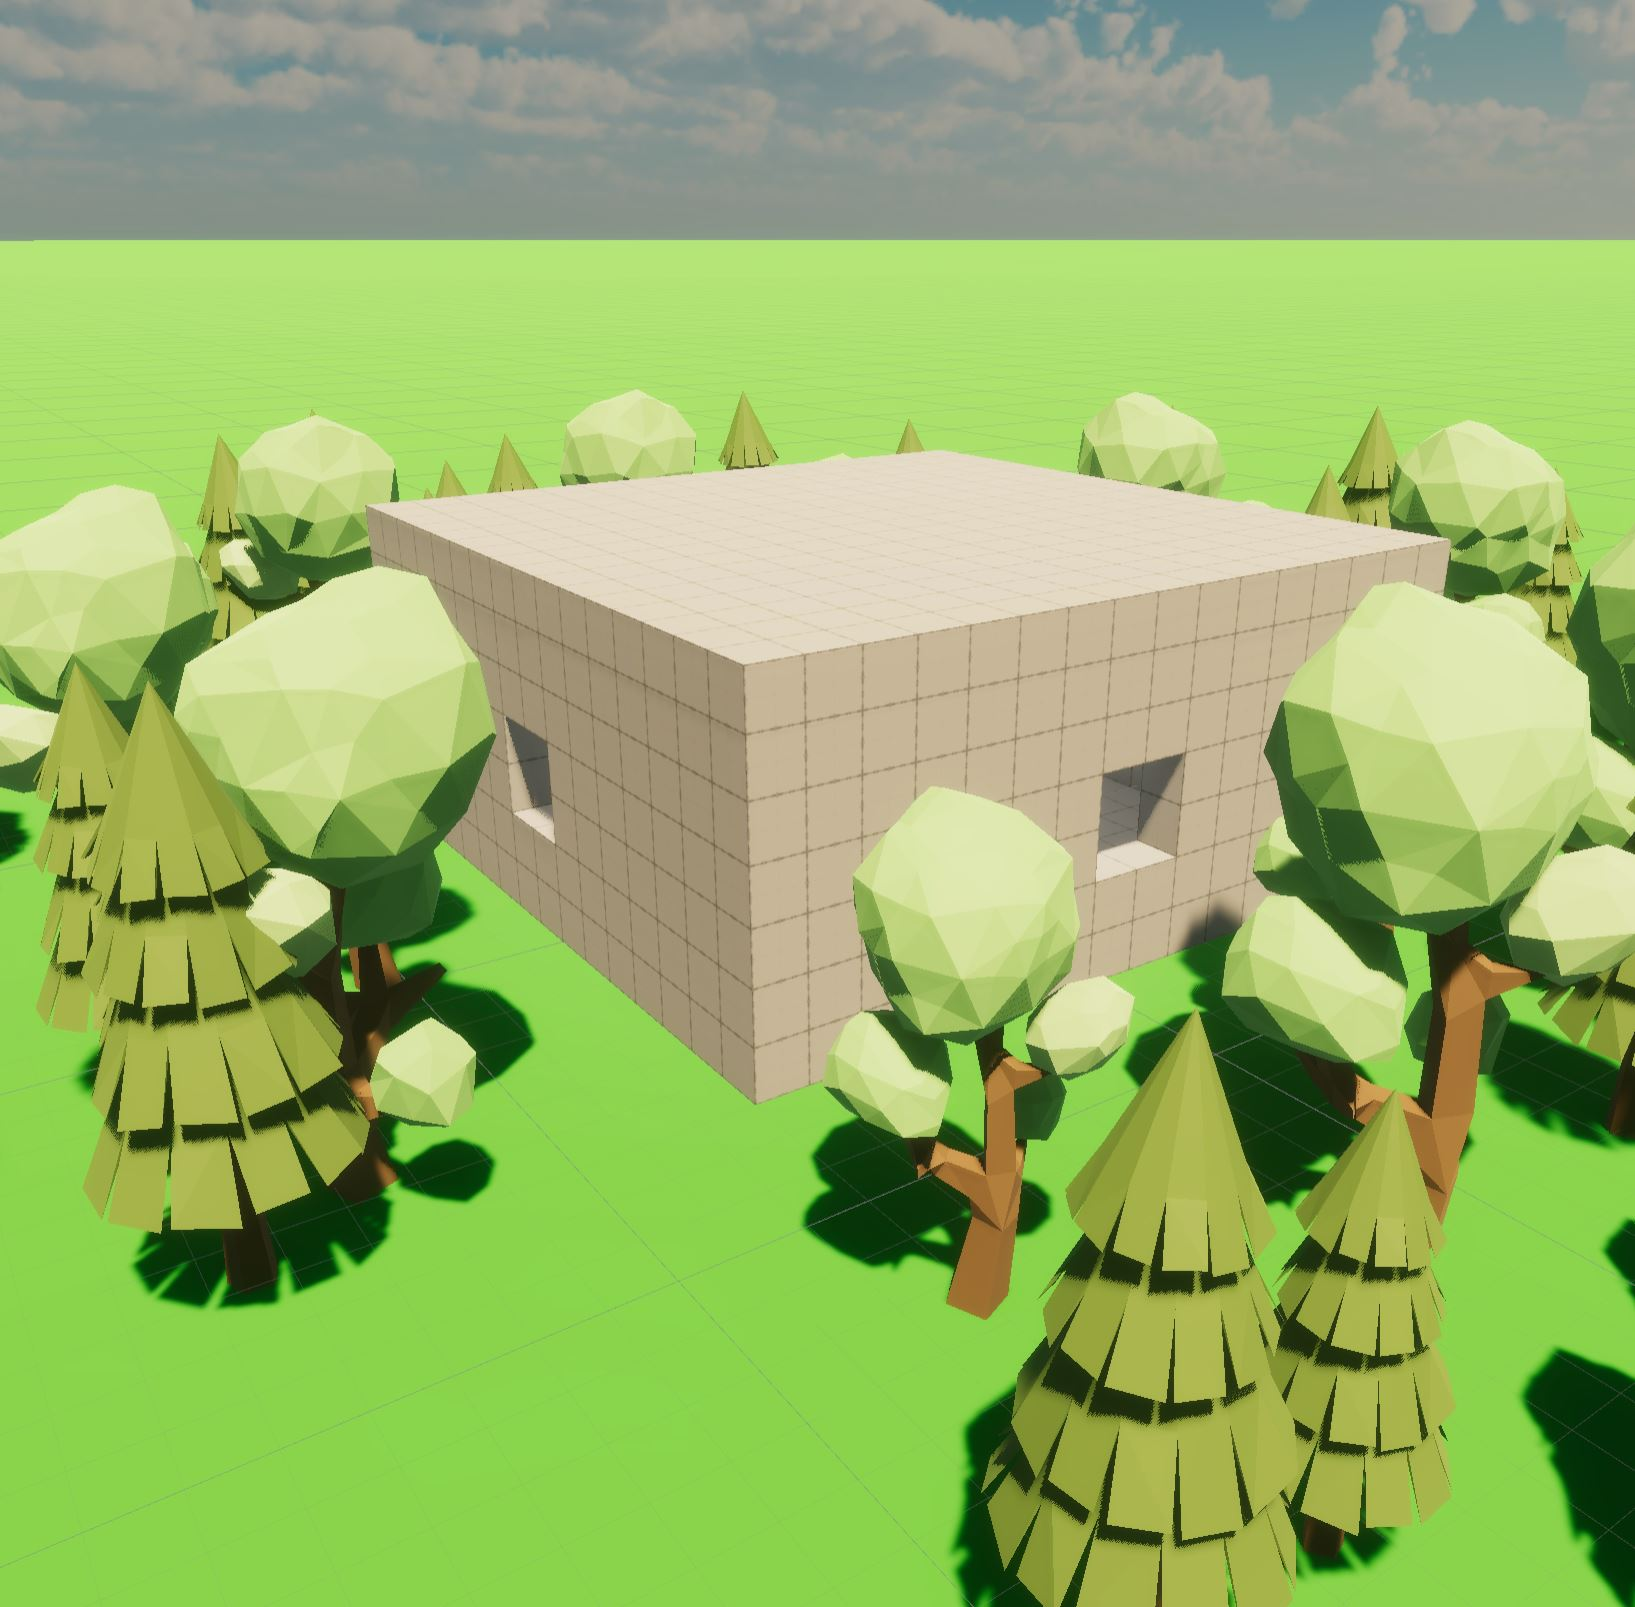
\includegraphics[scale=0.4]{Abbildungen/Versuchsumgebung/Raum.JPG}
			\caption[Die Versuchsumgebung von außen]{Die Versuchsumgebung von außen.}
			\label{Versuchsumgebung}
		\end{footnotesize}
	\end{figure}

\paragraph{Avatar-Konditionen}
Betritt ein Versuchsteilnehmer das \ac{sve}, bekommt dieser als Selbstrepräsentation nur seine eigenen, menschenähnlichen Hände zu sehen. Diese Ansicht ist unabhängig von den Konditionen \ac{ik} und \ac{nik}. Die Teilnehmer sehen folglich nur die jeweilige Avatar-Kondition der Mitspieler. 

\paragraph{Fade-to-Black und Positionsmanagement}
	Da sich alle Spieler im \ac{sve} frei bewegen können, müssen sie beim Spielstart vor ein Podest platziert werden. Startet der Spectator das Spiel, überprüft ein im globalen Datenspeicher liegendes Byte (die Bits des Bytes werden als Boolean genutzt), welche Podeste noch nicht belegt sind. Alle Mitspieler werden dementsprechend auf die freien Positionen vor die Podeste teleportiert. Damit es dem rot oder grün markierten Spieler nicht möglich ist, auf das Podest des erklärenden Spielers zu schauen, wurde ein Fade-to-Black Mechanismus implementiert. Entfernt sich ein Spieler von seinem Podest, wird sein Bild ab einem bestimmten Radius zunehmend schwärzer. Der Mechanismus funktioniert auch umgekehrt, sodass die Schwärze aus dem Bild verschwindet, sobald der Spieler sich wieder zu seinem Podest hin bewegt. Dasselbe Prinzip hält den erklärenden Spieler davon ab, die entsprechenden Symbole auf den Podesten seiner Mitspieler drücken zu können. Die Kommunikation der Spieler ist somit notwendig für die Vollendung einer Runde.

%\paragraph{Physical Handmodel, eigener Avatar war unsichtbar}
\paragraph{Animationen, Shadergraph und VFX-Graph}
Die Teilnehmer können im \ac{sve} lediglich die virtuellen Hände ihrer eigenen Körperrepräsentation sehen. Da die Hauptinteraktion das Drücken der Knöpfe des zugeteilten Podestes darstellt, soll dies für die Teilnehmer so einfach wie möglich gestaltet sein. Die teilnehmende Person soll sofort verstehen, wie diese mit seinem Avatar einen Knopf drücken kann. Die virtuellen Hände besitzen das Aussehen echter Hände mit einem hellgrauem Karo-Muster. Drückt eine teilnehmende Person den Triggerbutton seines Controllers, schließen sich alle Finger zu einer Faust.
Drückt ein Spieler einen der Symbol-Knöpfe, bekommt dieser durch eine gelbe Umrandung des Knopfes die Bestätigung, dass er den Knopf eingeloggt hat. Wird der Knopf erneut gedrückt, verschwindet die gelbe Umrandung. Diese Umrandungen leuchten im Ping-Pong-Effekt auf und wurden mit dem Unity Shader-Graph erstellt.
Die Teilnehmer sehen während einer Runde einen leuchtenden Ball zwischen den Podesten schweben, der aus einem Unitys VFX-Graph Partikelsystem besteht. Wird eine Runde beendet, wechselt die Farbe dieses Partikelsystems von Rot auf Grün und die Partikel werden auseinander geschleudert. 

\paragraph{PlayerHeight/Position Change}
Die unterschiedlichen Körpergrößen und unterschiedlichen Zimmergrößen der Versuchsteilnehmer müssen bei diesem Experiment berücksichtigt werden. Falls eine Person zu klein oder zu groß für das virtuelle Podest ist, kann dieser seine Spielerkamera und somit seinen Avatar mit den Tasten Q und E bis zu einem bestimmten Schwellenwert höher oder niedriger stellen. Durch diesen Mechanismus ist es auch sitzenden Personen möglich, an dem Versuch teilzunehmen. Falls das Zimmer zu klein oder aus anderen Gründen nicht genügend Platz vorhanden ist, um die Knöpfe auf dem Podest zu betätigen, können sich die Spieler sich zu einem gewissem Grad mit den Tasten W, A, S und D vorwärts, links, rechts und rückwärts in Blickrichtung bewegen.

\newpage	
\section{Statistische Auswertung}
Das folgende Kapitel beschäftigt sich mit der statistischen Auswertung. Jeder Hypothese ist ein eigenes Unterkapitel zugeordnet, in dem eine auf die jeweilige Hypothese zugeschnittene Auswertung stattfindet. Alle Ergebnisse wurden mit \textit{IBM SPSS Statistics} statistisch berechnet und ausgewertet (siehe \textit{Anhang \ref{Statistische Auswertung}}). 
Für jeden der hier aufgeführten Tests wurde eine Irrtumswahrscheinlichkeit von  $\alpha =,05$ festgelegt.

Die \textit{Tabelle \ref{VariableBreakdown1}} und die \textit{Tabelle \ref{VariableBreakdown2}} zeigen die verwendeten Methoden und Ergebnisse zur Auswertung der einzelnen Hypothesen im Überblick.

Die \textit{Tabelle \ref{MittelwerteUndCo}} zeigt eine deskriptive Statistik der relevantesten Variablen des Experiments.
	\subsection{Teilnehmer und Demografie}
Insgesamt nahmen 30 Personen an der Studie teil, sodass es insgesamt zehn Teams gab. 19 (63,3\%) Personen waren männlich und 11 (36,7\%) weiblich. Im Schnitt waren die Teilnehmer 30 Jahre alt $(\bar{x} = 30,13)$, wobei das 2. Quartil bei $28$ Jahren liegt.

\textit{Abbildung \ref{teilnehmer Alter}} zeigt die Altersstruktur sowie die Verteilung des biologischen Geschlechts der Personen, die an dem Experiment teilgenommen haben. 

	\begin{figure}[h]
  \centering
  \subfloat[][]{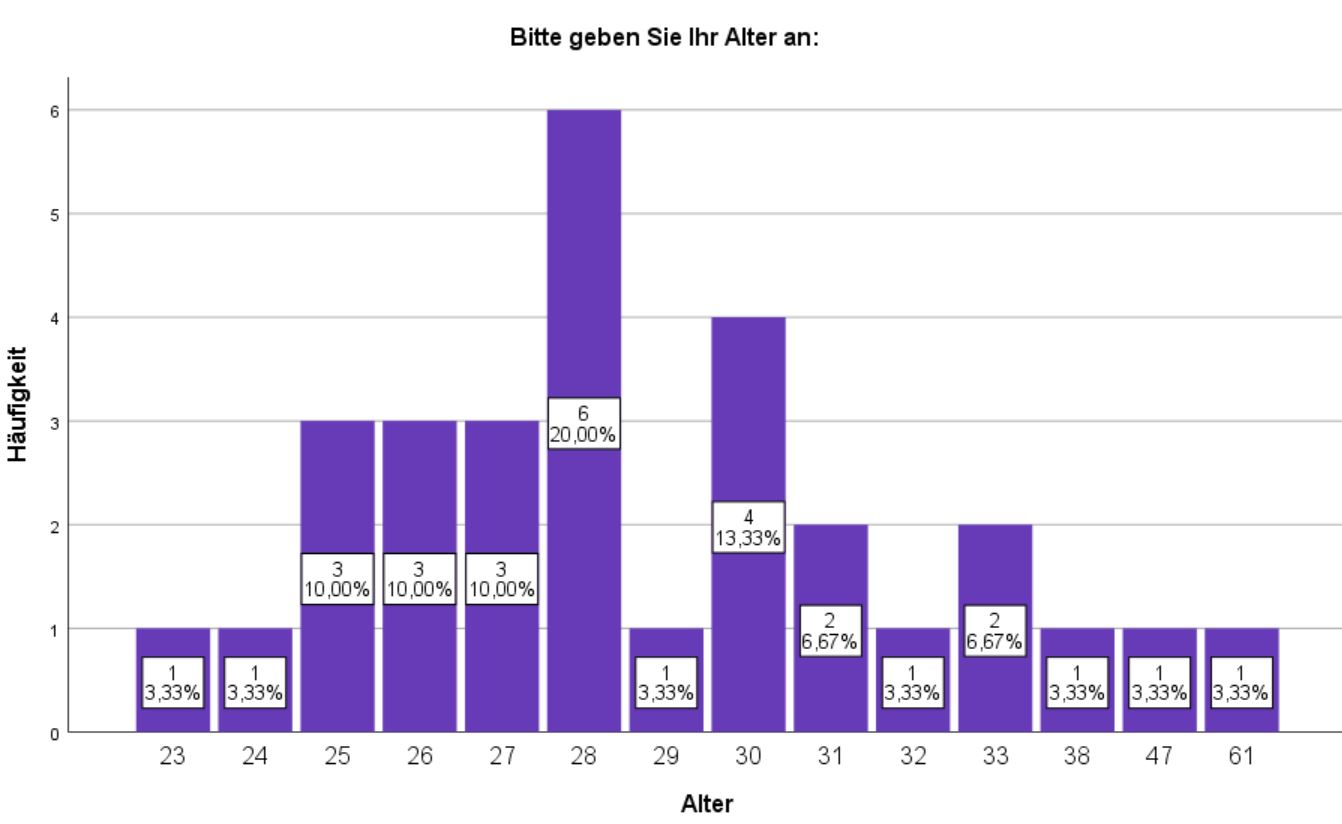
\includegraphics[width=0.47\linewidth]{Abbildungen/Demographie/alter.JPG}}
  \qquad
   \subfloat[][]{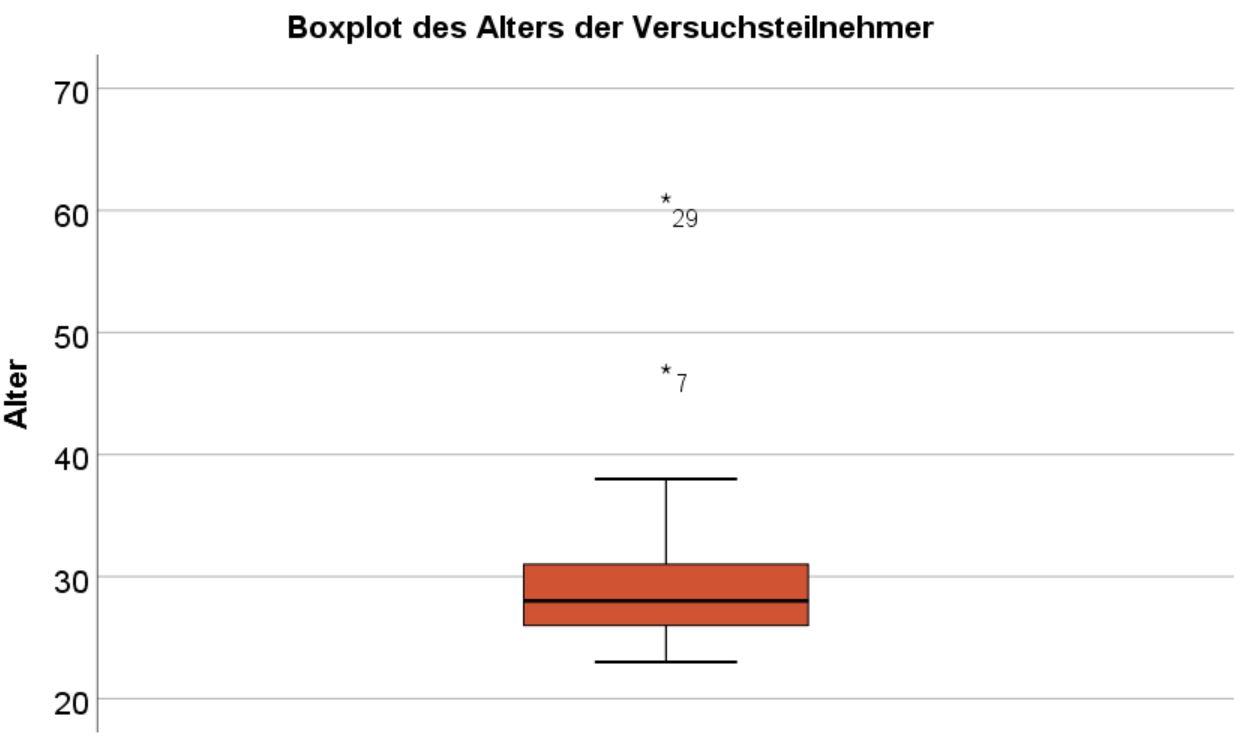
\includegraphics[width=0.47\linewidth]{Abbildungen/Demographie/Boxplot_Alter.JPG}}
  \qquad
  \subfloat[][]{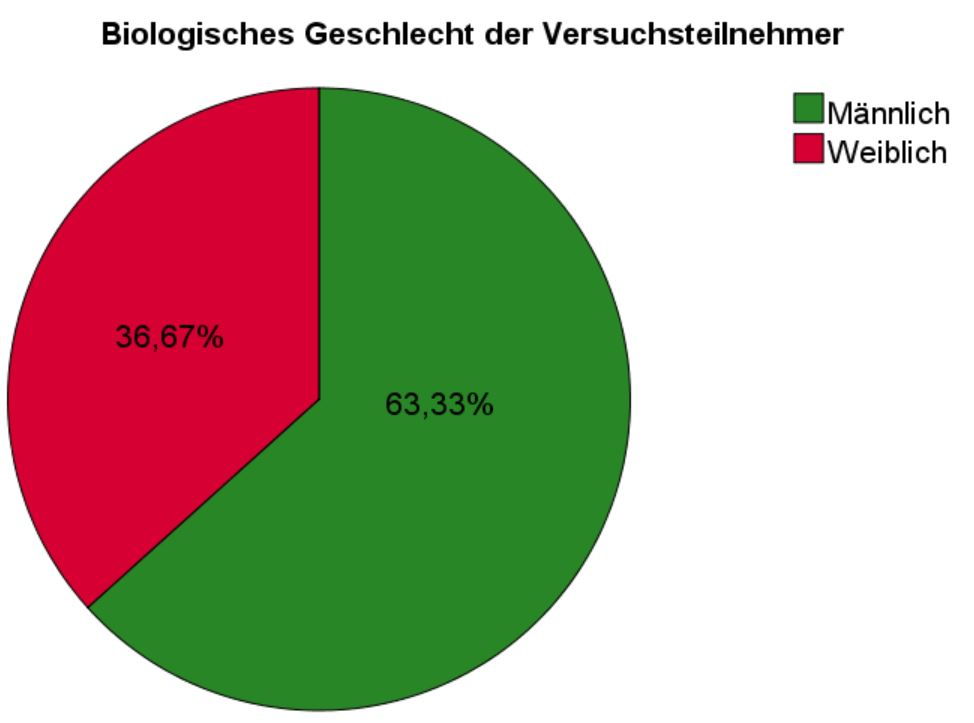
\includegraphics[width=0.40\linewidth]{Abbildungen/Demographie/teilnehmerGeschlecht.JPG}}
  \caption[Altersstruktur, Boxplot des Alters und biologisches Geschlecht der Teilnehmer]{Abbildung (a) zeigt die Altersstruktur der Personen, die an dem Experiment teilgenommen haben. Abbildung (b) zeigt den Boxplot der Altersstruktur der Versuchsteilnehmer. Abbildung (c) zeigt die Verteilung des biologischen Geschlechts der Personen, die an dem Experiment teilgenommen haben.}
  \label{teilnehmer Alter}
\end{figure}

Von den 30 Teilnehmern, besaß/en eine Person (3,3\%) das \textit{Fachabitur/Fachgebundene Hochschulreife}, 4 Personen (13,3\%) das \textit{Abitur/Allgemeine Hochschulreife}, 24 Personen (80\%) ein \textit{abgeschlossenes Studium} und eine Person (3,3\%) eine \textit{abgeschlossene Ausbildung} (siehe {\textit{Abbildung \ref{teilnehmerBildungsstand}}).

\begin{figure}[H]
		\begin{footnotesize}
		\centering
			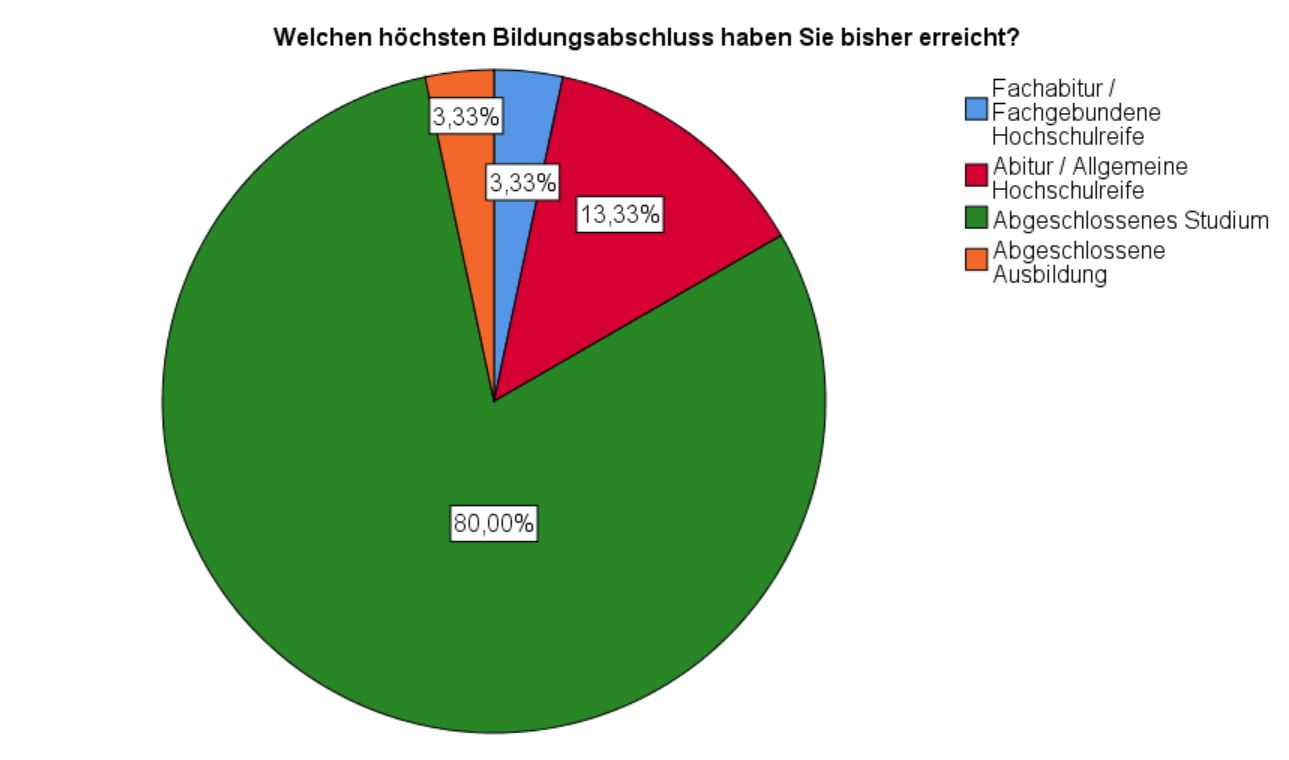
\includegraphics[scale=0.4]{Abbildungen/Demographie/teilnehmerBildungsstand.JPG}
			\caption[Der Bildungsstand der Teilnehmer]{Diese Abbildung zeigt den Bildungsstand der Teilnehmer, die an dem Experiment teilgenommen haben.}
			\label{teilnehmerBildungsstand}
		\end{footnotesize}
	\end{figure}

Deutlich mehr als die Hälfte der Teilnehmer (66,6\%) haben bereits Erfahrung in der \ac{vr} gesammelt. Von diesen Teilnehmern haben wiederum 23,3 Prozent (7 der 30 Teilnehmer) an \ac{vr}-Studien teilgenommen (siehe \textit{Abbildung \ref{teilnehmerVRErfahrungen}}).

\begin{figure}[h]
  \centering
  \subfloat[][]{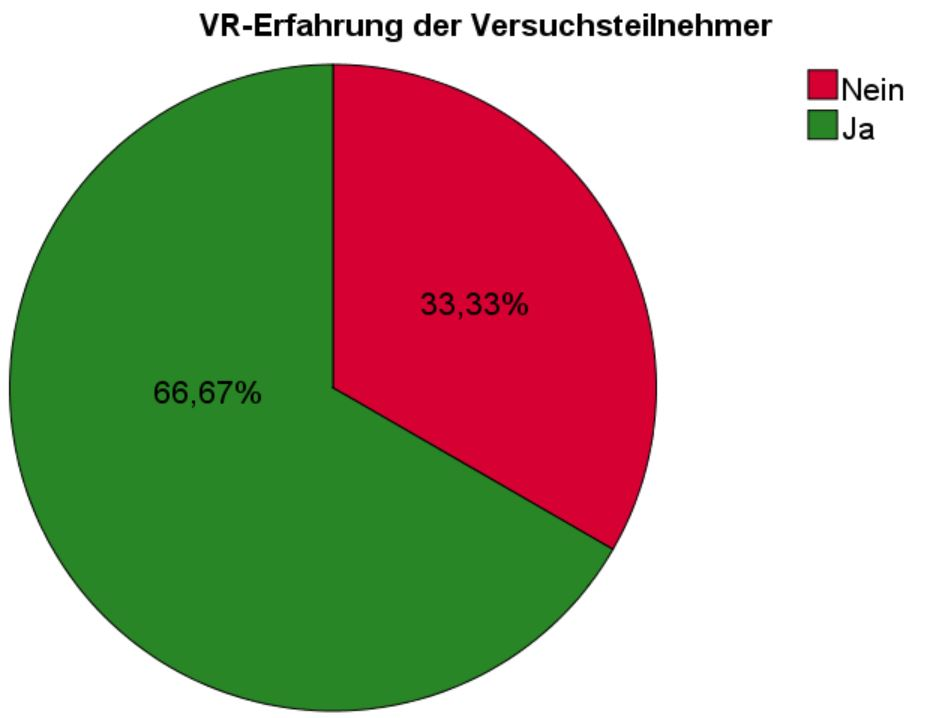
\includegraphics[width=0.4\linewidth]{Abbildungen/Demographie/teilnehmerVRErfahrung.jpg}}
  \qquad
  \subfloat[][]{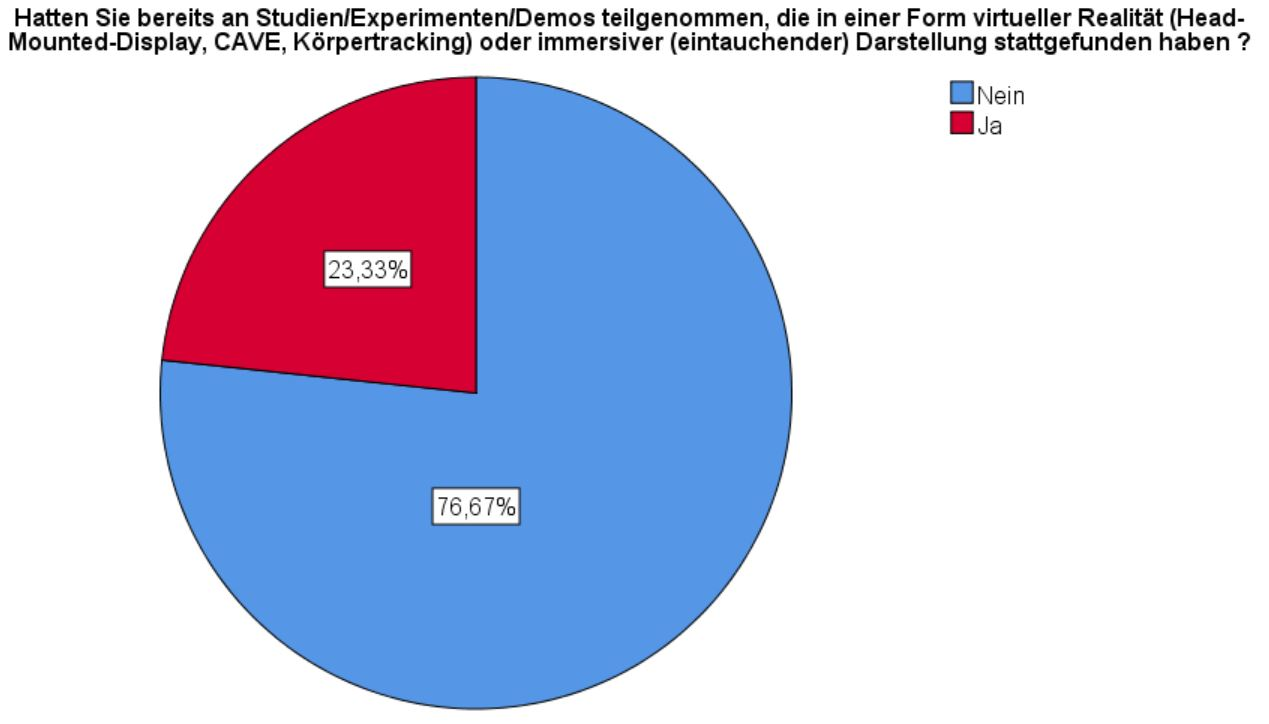
\includegraphics[width=0.4\linewidth]{Abbildungen/Demographie/teilnehmerVorexperimente.jpg}}
  \caption[Die vorhandene VR-Erfahrung der Teilnehmer]{Diese Abbildung zeigt die VR Erfahrung (a) und die VR-Studien Erfahrung (b) der Teilnehmer.}
  \label{teilnehmerVRErfahrungen}
\end{figure}

Mittels einer Likert-Skala von 1-7 (1 = wenig, 7 = sehr viel) wurde nach dem Ausmaß der Internetnutzung im täglichen Leben gefragt. Dabei gab der Großteil (70\%) der Teilnehmer an, dass diese das Internet \textit{sehr viel} nutzen.

Mittels einer weiteren Likert-Skala von 1-7 (1 = wenig, 7= sehr viel) wurde danach gefragt, wie häufig die Teilnehmer Videospiele spielen. Der Mittelwert der Likert-Skala beträgt 3,5, wobei im 50\% Perzentil das Videospiel-Ausmaß mit \grqq 3\grqq{} beziffert wurde. Der Mittelwert betrug ($\bar{x} = 3,1$) und liegt damit ebenfalls unter dem Durchschnitt.
\textit{Abbildung \ref{teilnehmerInternetVideospiele}} zeigt das Ausmaß der Internetnutzung und das Ausmaß des Videospielkonsums der Teilnehmer.
\begin{figure}[h]
  \centering
  \subfloat[][]{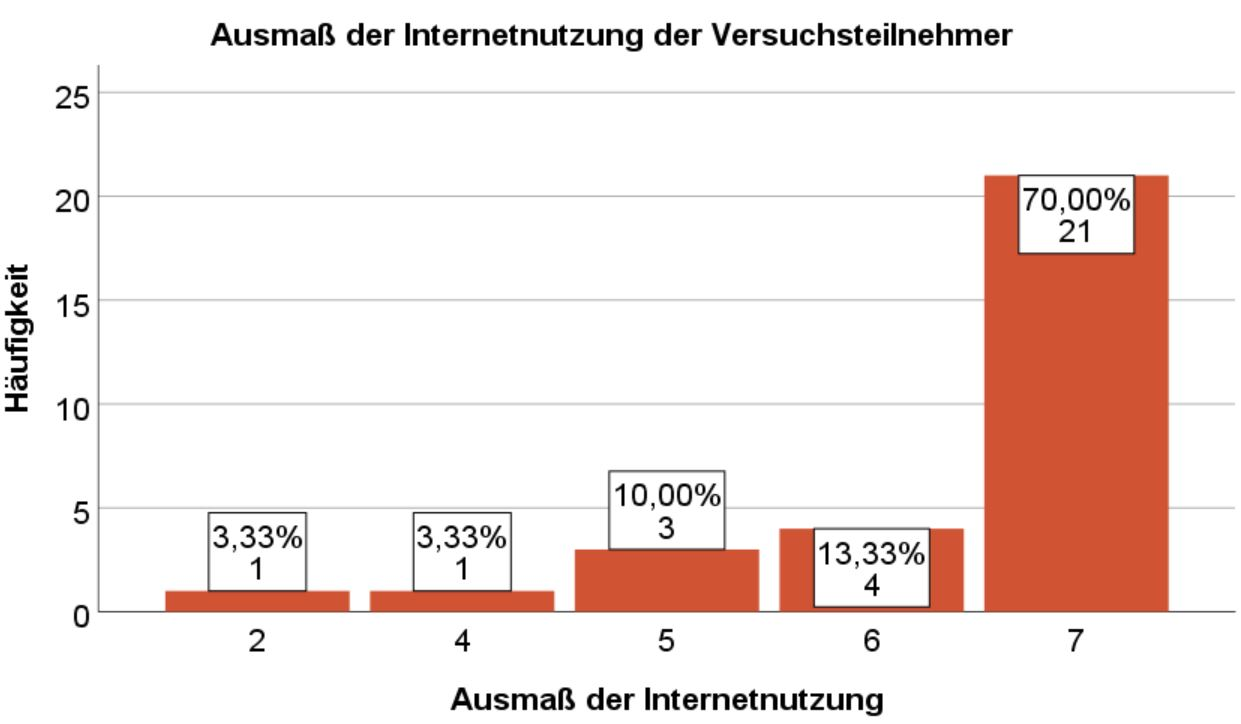
\includegraphics[width=0.6\linewidth]{Abbildungen/Demographie/teilnehmerPCAußmaß.jpg}}
  \qquad
  \subfloat[][]{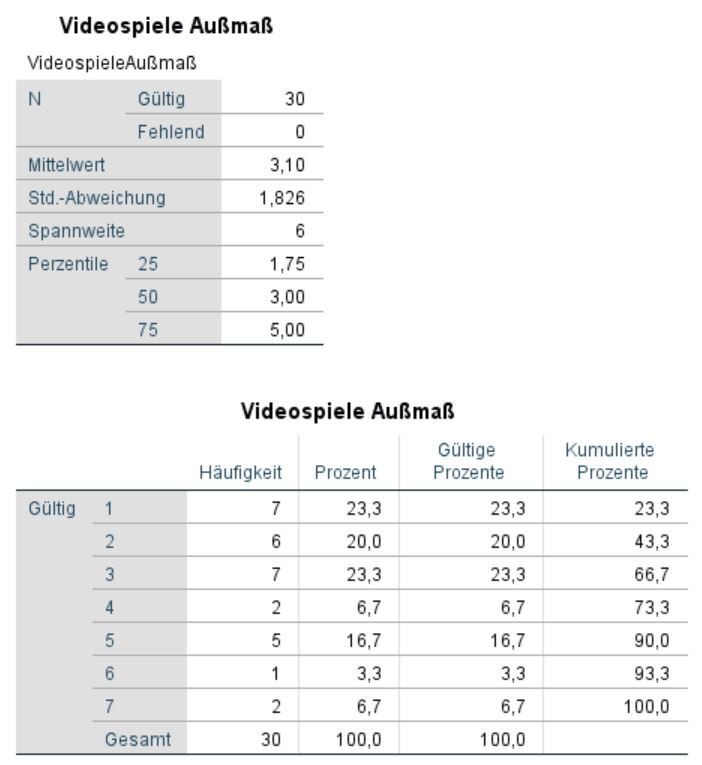
\includegraphics[width=0.6\linewidth]{Abbildungen/Demographie/teilnehmerVideospieleAußmaß.jpg}}
  \caption[Das Ausmaß der Internetnutzung und des Videospielkonsums der Teilnehmer]{Diese Abbildungen zeigen das Ausmaß der Internetnutzung (a) und das Ausmaß des Videospielkonsums (b) der Teilnehmer.}
  \label{teilnehmerInternetVideospiele}
\end{figure}

%	\subsection{Voraussetzungen}
	
%\paragraph{Anzahl abgeschlossener Runden}
%Die maximale Anzahl an abgeschlossenen Runden beträgt 13. Die minimale Anzahl 4. Um in einem Wertebereich zwischen 0 und 1 zu bleiben, wurde die Anzahl an abgeschlossenen Runden im Vorhinein normalisiert.
%Siehe \textbf{\autoref{fig:boxplot_cognitive_trust_winsorisiert}}. 
%\ac{gt} ist unabhängig vom \ac{ct} der einzelnen Testperson. Es muss eine Spearman-Korrelation auf Individualebene mit $N=30$ Personen durchgeführt werden, bei der die einzelnen Teams und Teamzusammensetzungen sowie die Avatar-Konditionen ignoriert werden. 
%	
%\paragraph{Test auf Normalverteilung der Daten}
%Für viele Tests ist eine Voraussetzung, dass die Stichproben Normalverteilt sind. Zur Überprüfung auf Normalverteilung wurde der \textit{Kolmogoroff-Smirnov-Test} genutzt. Die Null-Hypothese dieses Tests besagt, dass eine Normalverteilung der Variablen vorliegt. Wenn ($p < \alpha = ,05$), muss H0 verworfen werden und angenommen werden, dass die Daten nicht Normalverteilt sind.
%
%Bei kleinen Stichproben kann ebenfalls die Skewness und die Kurtosis genutzt werden, um auf Normalverteilung zu überprüfen. 
%Die Schiefe und die Kurtosis sollten "nahe Null" sein, damit man von einer normalverteilten Variable ausgehen kann.\\
%$ z_{Skewness} = \frac{S-0}{\sigma_{Skewness}} $ \\
%$ z_{Kurtosis} = \frac{K-0}{\sigma_{Kurtosis}} $ \\
%$\sigma_{Kurtosis}$ sowie $\sigma_{Skewness}$ werden von SPSS ausgegeben. $S$ ist die Skewness, $K$ ist die Kurtosis und ${\sigma_{(Skewness/Kurtosis)}}$ ist die Standardabweichung.
%Um " nahe Null " zu bestimmen, können die mit vorheriger Formel bestimmten Werte mit den folgenden Grenzwerten verglichen werden:
%Für kleine Stichproben (n < 50) : ($z < |+/-1.96|$) ist \textbf{signifikant} mit $p<0.05$. \newline
%Für mittlere Stichproben (50 < n < 100) : ($z < |+/-2.58|$) ist \textbf{signifikant} mit $p<0.01$. \newline
%Für mittlere Stichproben (n > 100) : ($z < |+/-3.29|$) ist \textbf{signifikant} mit $p<0.001$. \newline
%Ist der jeweilige z-Wert größer als dieser Grenzwert muss die Nullhypothese verworfen werden und von nicht normalverteilen Daten ausgegangen werden \citep[S. 184]{field2013discovering}.
%
%\paragraph{T-Test}
%Um zu überprüfen, ob sich zwei  Gruppen unterscheiden, muss ein t-Test für unabhängige Variablen durchgeführt werden.
%Dieser hat die Voraussetzung, dass die Stichproben \textbf{unabhängig}, \textbf{intervallskaliert}, \textbf{Normalverteilt} sowie eine \textbf{ähnlich gleiche Varianz} besitzen.
%
%\paragraph{Mann-Whitney-U-Test}
%Dieser Test ist im Gegensatz zum t-Test eher unanspruchsvoll. Die Messungen der einen Gruppe dürfen nicht durch Messungen der anderen Gruppe beeinflusst sein. Somit müssen die Messungen \textbf{unabängig} sein. Die unabhängige Variable ist \textbf{nominalskaliert} und besitzt \textbf{zwei Ausprägungen}. Die \textbf{abhängige Variable} ist mindestens \textbf{ordinalskaliert}  und die Gruppen müssen etwa die gleiche Verteilung besitzen \citep{eid2017statistik}.

\clearpage
\newpage	
	\subsection{Auswertung Hypothese 1}
	\label{Auswertung Hypothese 1}
%H1$_{0}$ : Die Mittelwerte der erzielten \textit{kognitiven Vertrauenswerte} unterscheiden sich bei den Konditionen \ac{ik} und \ac{nik} nicht signifikant voneinander.

\paragraph{Allgemeines}
Auf \textit{Konditionsebene} wird analysiert, ob die Teilnehmer aufgrund der unterschiedlichen Avatar-Konditionen unterschiedliches \textit{kognitives Vertrauen} bilden. Dazu wird der Mann-Whitney-U-Test durchgeführt.\\
Das \textit{kognitive Vertrauen} ist laut dem Shapiro-Wilk-Test\footnote{Der Shapiro-Wilk-Test ist ein Signifikanztest, der überprüft, ob eine Grundgesamtheit Normalverteilt ist \citep[S. 25]{razali2011power}.} mit $p =,002 < \alpha =,05$ \textit{nicht normalverteilt}.
%Es wurde auf Varianzgleichheit überprüft. Der Levene-Test zeigt eine Varianzgleichheit zwischen \ac{cti} und \ac{ctn} ($L =,889; p=.354 > \alpha = ,05$). Damit kann davon ausgegangen werden, dass die Varianzen sich \textbf{nicht signifikant} voneinander unterscheiden.\\
%\paragraph{Mittelswerte und Standardabweichungen}
Der angegebene \textit{kognitive Vertrauenswert} der Kondition \ac{ik} beträgt im Mittel $\bar{x} = 4,188$ mit einer Standardabweichung von $\sigma =,651$.\newline 
Der angegebene \textit{kognitive Vertrauenswert} der Kondition \ac{ik} beträgt im Mittel $\bar{x} = 4,622$ mit einer Standardabweichung von $\sigma =,347$ (siehe \textit{Abbildung \ref{SD_kognitivesVertrauenBP}} und \textit{Abbildung \ref{H1_Mittelwerte_Auswertung}}).

\paragraph{Mann-Whitney-U-Test}
%Aufgrund des geringen p-Wertes des \ac{cti} im Kolmogoroff-Smirnov-Test mit ($p =,185 > \alpha = ,05$) wurde zusätzlich noch der Mann-Whitney-U-Test durchgeführt.
Die Verteilungsformen der beiden Konditionen unterscheiden sich laut Kolmogorov-Smirnov ($p =,925 > \alpha =,05$) \textbf{nicht signifikant} voneinander. Es gab laut Mann- Whitney-U-Test \textbf{einen signifikanten Unterschied} zwischen den Mittelwerten der \textit{kognitiven Vertrauenswerte} der Avatar-Konditionen \ac{ik} $(\bar{x} = 4,188)$ und \ac{nik} $(\bar{x} = 4,622)$ mit $U = 64,000; Z = -2,029; p =,042 < \alpha =,05; r =-,370$. \\

	\begin{figure}[H]
   \begin{minipage}[t]{.5\linewidth} % [b] => Ausrichtung an \caption
      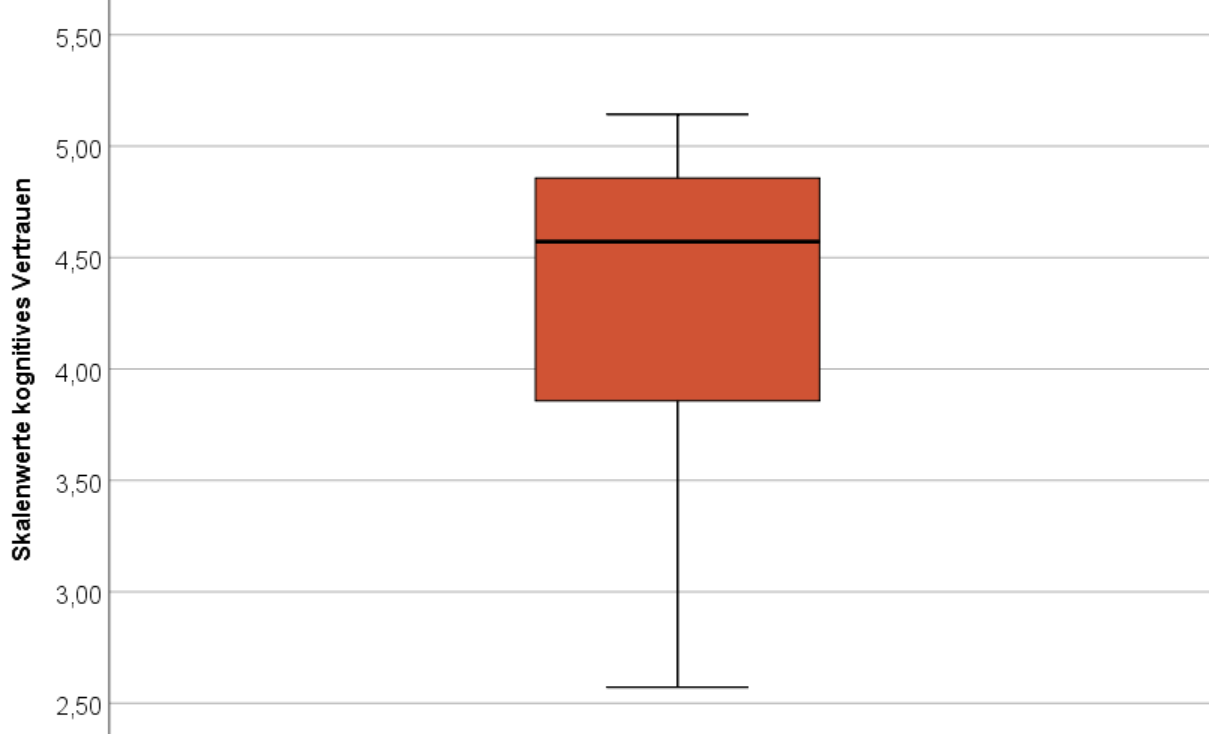
\includegraphics[width=\linewidth]{Abbildungen/AuswertungDiagramme/Final/BP_kognitivesVertrauen.png}
      \caption[Boxplot der kognitiven Vertrauenswerte der Versuchsteilnehmer]{Boxplot der kognitiven Vertrauenswerte der Versuchsteilnehmer.}
            \label{SD_kognitivesVertrauenBP}
   \end{minipage}
   \hspace{.02\linewidth}% Abstand zwischen Bilder
   \begin{minipage}[t]{.5\linewidth} % [b] => Ausrichtung an \caption
     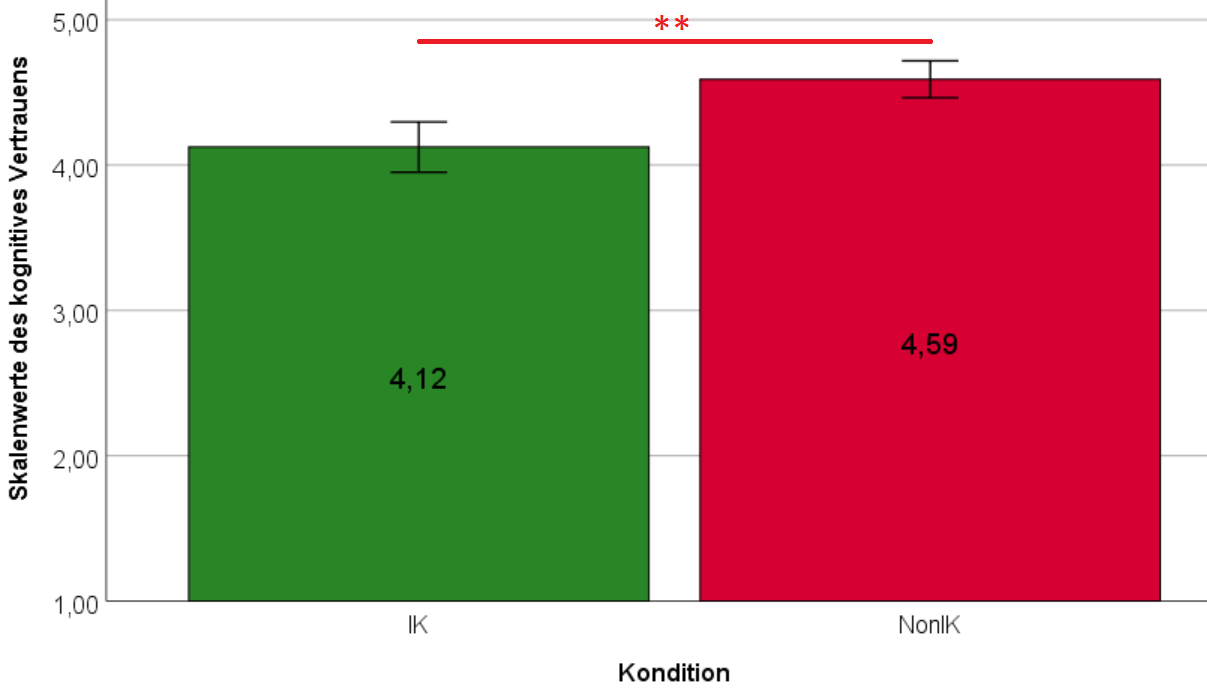
\includegraphics[width=\linewidth]{Abbildungen/AuswertungDiagramme/Final/H1_Mittelwerte.png}
      \caption[Mittelwerte und der Standardfehler der kognitiven Vertrauenswerte]{Die durchschnittlichen Ergebnisse des wahrgenommenen kognitiven Vertrauens der Avatar-Konditionen. Die Fehlerbalken zeigen die Standardfehler. Links die Kondition \ac{ik} und rechts die Kondition \ac{nik}. $** : p < \alpha =,05$}
       \label{H1_Mittelwerte_Auswertung}
   \end{minipage}
\end{figure}

\newpage
\subsection{Auswertung Hypothese 2}
\label{Auswertung Hypothese 2}
%H1$_{0}$ : Steigt der General-Trust-Score einer Person (\ac{gt}), steigt der Cognitive-Trust-Score einer Person (\ac{ct}) nicht.
%H2$_{0}$ : Es besteht kein signifikanter Zusammenhang zwischen dem erzielten \textit{generellen Vertrauenswert} einer Person und dem erzielten \textit{kognitiven Vertrauenswert} einer Person.

\paragraph{Allgemeines}
Es wird analysiert, ob ein Zusammenhang zwischen dem \textit{generellen Vertrauenswert} und dem \textit{kognitiven Vertrauenswert} auf Konditionsebene besteht.\\
Der \textit{kognitive Vertrauenswert} muss für \textit{Hypothese 1} auf \textit{Konditionsebene} analysiert werden, da der \textit{kognitive Vertrauenswert} aufgrund der unterschiedlichen Avatar-Konditionen gebildet wurde. Somit ist es nicht möglich, den Zusammenhang zwischen dem \textit{generellen Vertrauenswert} und dem \textit{kognitiven Vertrauenswert} auf \textit{Individualebene} zu betrachten.

Der Shapiro-Wilk-Test zeigt, dass der \textit{generelle Vertrauenswert} der Kondition \ac{ik} mit $p =,382 > \alpha =,05$ \textit{normalverteilt} und der \textit{generelle Vertrauenswert} der Kondition \newline \ac{nik} mit $p =,944 > \alpha =,05$ \textit{normalverteilt} ist.

Aus einem weiteren Shapiro-Wilk-Test geht hervor, dass der \textit{kognitive Vertrauenswert} der Kondition \ac{ik} mit  $p =,183 > \alpha = ,05$ \textit{normalverteilt} und der \textit{kognitive Vertrauenswert} der Kondition \ac{nik} mit $p =,069 > \alpha =,05$ \textit{normalverteilt} ist.
Das Lowess-Verfahren\footnote{Das Lowess-Verfahren (Locally-Weighted Scatterplot Smoother) ist ein Verfahren, dass mittels einer lokal gewichteten Regressionsfunktion den Zusammenhang zweier oder mehrerer Variablen visuell ermöglicht.} deutet augenscheinlich auf keinen linearen Zusammenhang zwischen dem \textit{generellen Vertrauenswert} der Kondition \ac{ik} und dem \textit{kognitiven Vertrauenswert} der Kondition \ac{ik} sowie dem \textit{generellen Vertrauenswert} der Kondition \ac{nik} und dem \textit{kognitiven Vertrauenswert} der Kondition \ac{nik} hin. Daher wird die Linearitätsannahme abgelehnt.

%Für \ac{gt} ist $ z_{Skewness} = -0,985 $ und $z_{Kurtosis} = -.416$ und somit ist \ac{gt} normalverteilt.
%Für \ac{ct} ist $ z_{Skewness} = -.257 $ und $z_{Kurtosis} = -1,764$ und somit ist \ac{ct} normalverteilt.
%Voraussetzung für Pearson-Korrelationsanalyse: 
%Die Variablen sind mindestens intervallskaliert -> Hier ordinalskaliert
%Die Variablen sind normalverteilt -> JA
%Der untersuchte Zusammenhang zwischen den Variablen muss linear sein -> JA
%Ab einer Likert Skala ab 6 können ordinale Skalenniveaus als metrische variablen interpretiert werden???
%\paragraph{Pearson-Korrelationsanalyse}
%Es ist eine positive Korrelation starken Effektes (vgl. \cite{cohen2013statistical}) mit dem Pearson-Korrelationskoeffizient ($r =,522$) zwischen \ac{gti} und \ac{cti} vorhanden. Die Pearson-Korrelation ist \textbf{nicht signifikant} ($p =,055 > \alpha = ,05$).\\
%Weiterhin ist eine positive Korrelation moderaten Effektes (vgl. \cite{cohen2013statistical}) mit dem Pearson-Korrelationskoeffizient ($r =,306$) zwischen \ac{gtn} und \ac{ctn} vorhanden. Die Pearson-Korrelation ist \textbf{nicht signifikant} ($p =,267 > \alpha = ,05$).

\begin{figure}[h]
  \centering
  \subfloat[][]{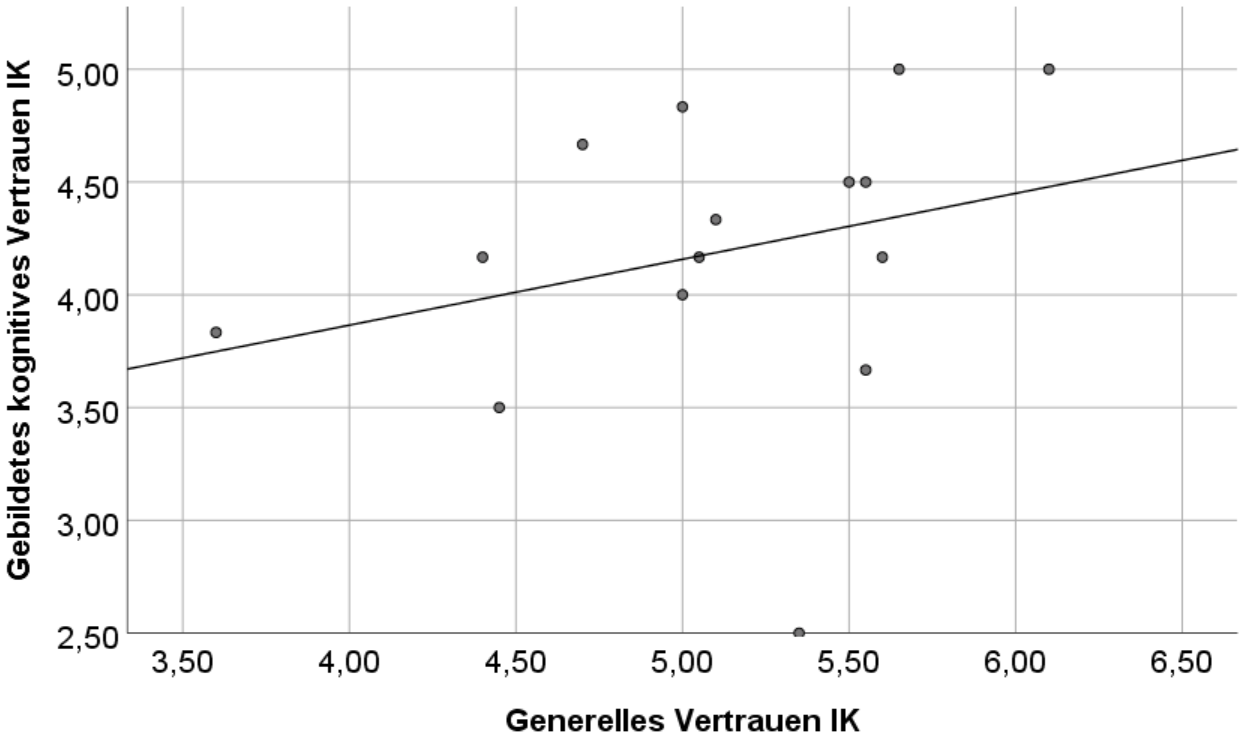
\includegraphics[width=0.45\linewidth]{Abbildungen/AuswertungDiagramme/Final/H_2_KorrIK.png}}
  \qquad
  \subfloat[][]{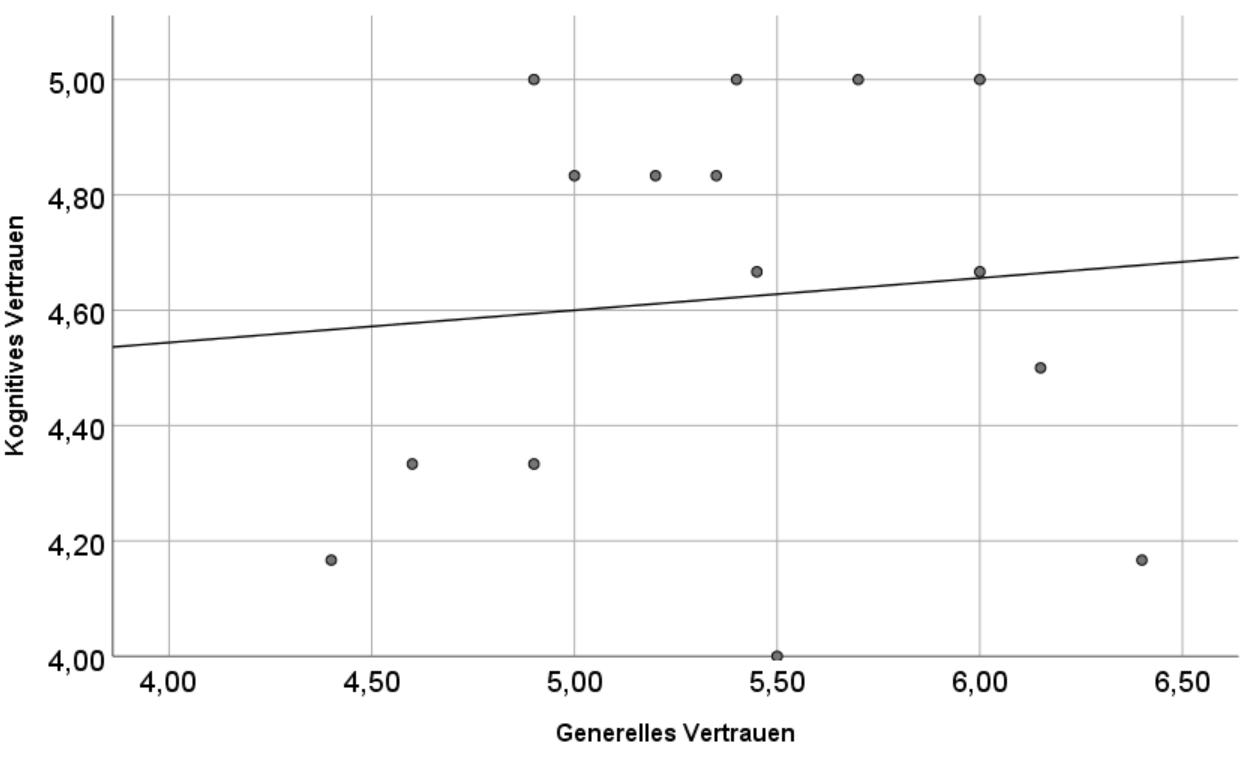
\includegraphics[width=0.45\linewidth]{Abbildungen/AuswertungDiagramme/Final/H_2_KorrNIK.png}}
    \qquad
  \subfloat[][]{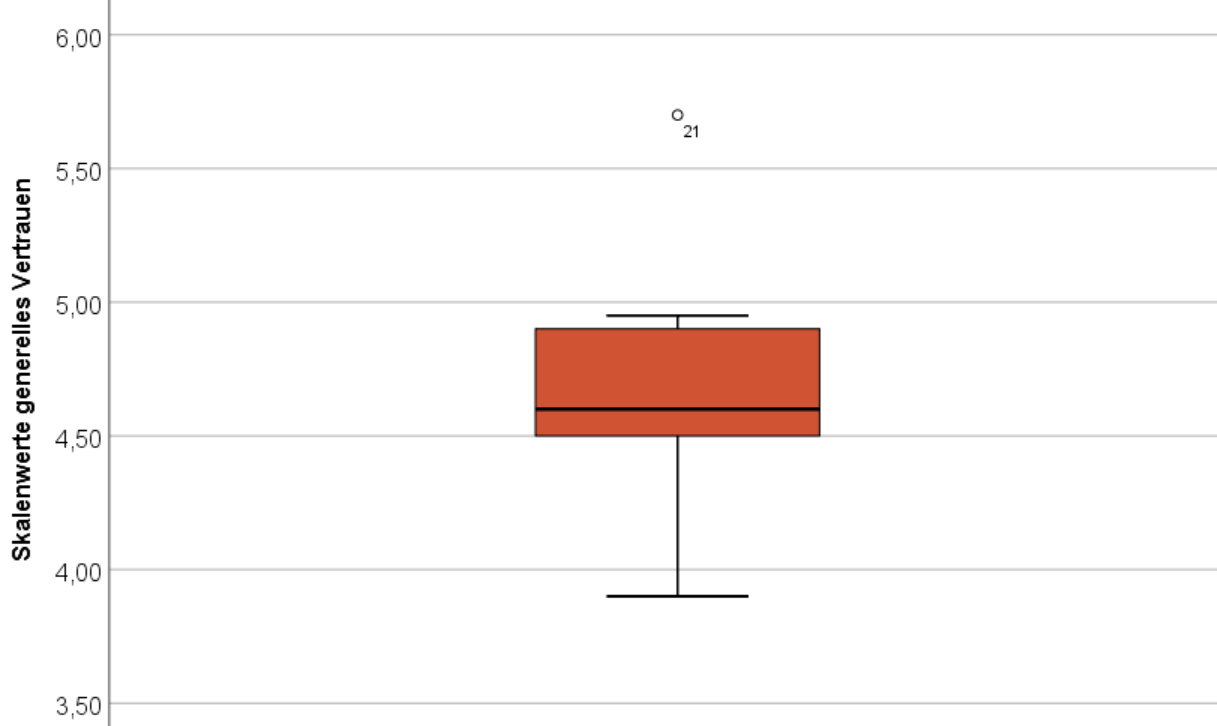
\includegraphics[width=0.45\linewidth]{Abbildungen/AuswertungDiagramme/Final/BP_generellesVertrauen.png}}
  \caption[Korrelationen der generellen Vertrauenswerte mit den kognitiven Vertrauenswerten]{Korrelationen der generellen Vertrauenswerte mit den kognitiven Vertrauenswerten. Links (a) für die Kondition \ac{ik} und rechts (b) für die Kondition \ac{nik}. (c) stellt den Boxplot der generellen Vertrauenswerte der individuellen Personen dar.}
  \label{H2_Korrelation_Auswertung}
\end{figure}
\newpage
\paragraph{Spearman-Korrelationsanalyse}
Es ist eine positive starke Korrelation (vgl. \citep{cohen2013statistical}) mit dem Spearman-Korrelationskoeffizient $r =,406$ zwischen dem \textit{generellen Vertrauenswert} der Kondition \ac{ik} und dem \textit{kognitiven Vertrauenswert} der Kondition \ac{ik} vorhanden. Die Spearman-Korrelation ist \textbf{nicht signifikant} ($p =,134 > \alpha =,05$).

Weiterhin liegt eine positive Korrelation schwacher Stärke (vgl. \citep{cohen2013statistical}) mit dem Spearman-Korrelationskoeffizient $r = ,045$ zwischen dem \textit{generellen Vertrauenswert} der Kondition \newline \ac{nik} und dem \textit{kognitiven Vertrauenswert} der Kondition \ac{nik} vor. Die Spearman-Korrelation ist \textbf{nicht signifikant} ($p = ,872 > \alpha = ,05$) (siehe \textit{Abbildung \ref{H2_Korrelation_Auswertung}}).

\paragraph{Fisher-Z-Transformation für unabhängige Stichproben}
Um herauszufinden, ob sich beide Korrelationen signifikant voneinander unterscheiden, wird eine Fisher-Z-Transformation für unabhängige Stichproben durchgeführt.
Die beiden Korrelationen unterscheiden sich laut Fisher-Z-Wert für unabhängige Stichproben ($Z =,954$) \textbf{signifikant} voneinander ($p =,017 < \alpha =,05$).

\newpage
\clearpage
\subsection{Auswertung Hypothese 3}
\label{Auswertung Hypothese 3}
%\textbf{H3$_{0}$} : Der Zusammenhang zwischen dem \textit{kognitiven Vertrauenswert von Teams} und der \textit{Teameffektivität von Teams} mit der Kondition \ac{ik} unterscheiden sich nicht signifikant von den Teams mit der Kondition \ac{nik}.
\paragraph{Allgemeines}
Es wird der Zusammenhang zwischen dem \textit{kognitiven Vertrauenswert von Teams} und der \textit{Teameffektivität von Teams} auf Teamebene analysiert.

\paragraph{Vertrauenstabelle pro Team}
%Es wird der Zusammenhang zwischen \ac{cti} und \ac{tRoundIK} sowie \ac{ctn} und \ac{tRoundNIK} auf Teamebene analysiert.
In einem Versuchsdurchlauf besitzt jedes der 3 Teammitglieder die gleiche Avatar-Kondition. Die Anzahl der abgeschlossenen Runden jedes einzelnen Teams bildet die \textit{Teameffektivität des Teams}. 
Für jedes Team wird zudem ein gemeinsamer kognitiver Vertrauenswert berechnet. Dieser sagt aus, wie viel \textit{kognitives Vertrauen} das gesamte Team gebildet hat und ergibt sich aus der Summe der \textit{kognitiven Vertrauenswerte} der einzelnen Personen eines Teams. Dieser wurde für jedes einzelne Team derselben Kondition zusammengefasst (siehe \textit{Tabelle \ref{TeamCogTabelle}})

Im Anschluss wird eine Spearman-Korrelation zwischen der \textit{Teameffektivität} und den \textit{kognitiven Vertrauenswerten} auf \textit{Teamebene} durchgeführt, wobei die Teams in verschiedene Konditionen aufgeteilt werden. Damit anschließend überprüft werden kann, ob sich beide Korrelationen voneinander unterscheiden, wird eine Fisher-Z-Transformation für unabhängige Stichproben durchgeführt.\\
%Somit müssen die kognitiven Vertrauenswerte nicht winsorisiert werden. 
%Alle Ergebnisse werden in \ac{ik} und \ac{nik} aufgeteilt um ein Vergleich der verschiedenen Konditionen darzustellen. Kondition 1 definiert die Kondition \ac{ik} und Kondition 2 definiert die Kondition \ac{nik}.
%
Die \textit{kognitiven Vertrauenswerte der Teams} mit der Kondition \ac{ik} sind laut Shapiro-Wilk-Test mit $p =,109 > \alpha = ,05$ normalverteilt. \newline
Die \textit{kognitiven Vertrauenswerte der Teams} mit der Kondition \ac{nik} sind laut Shapiro-Wilk-Test mit $p =,278 > \alpha = ,05$ normalverteilt. \newline
Die \textit{Teameffektivität der Teams} mit der Kondition \ac{ik} ist laut Shapiro-Wilk-Test mit $p =,844 > \alpha = ,05$ normalverteilt. \newline
Die \textit{Teameffektivität der Teams} mit der Kondition \ac{nik} ist mit $p =,453 > \alpha = ,05$ normalverteilt. \\
Das Lowess-Verfahren deutet augenscheinlich auf keinen linearen Zusammenhang zwischen den \textit{kognitiven Vertrauenswerten der Teams} mit der Kondition \ac{ik} und der \textit{Teameffektivität der Teams} mit der Kondition \ac{ik} sowie auf keinen linearen Zusammenhang zwischen den \textit{kognitiven Vertrauenswerten der Teams} mit der Kondition \ac{ik} und der \textit{Teameffektivität der Teams} mit der Kondition \ac{nik} hin. Daher wird die Linearitätsannahme abgelehnt.

Aufgrund des geringen Stichprobenumfangs der einzelnen Teams der verschiedenen Avatarkonditionen ($N=5$) und der nicht eindeutigen Linearität durch das Lowess-Verfahren, wurde sich für eine Spearman-Korrelation entschieden.

\paragraph{Spearman-Korrelation}

Der Spearman-Korrelationskoeffizient zwischen den \textit{kognitiven Vertrauenswerten der Teams} mit der Kondition \ac{ik} und der \textit{Teameffektivität der Teams} mit der Kondition \ac{ik} beträgt $r =,205$ Diese Korrelation moderater Stärke ist positiv (vgl. \citep{cohen2013statistical}) und ist \textbf{nicht signifikant} ($p =,741 > \alpha = ,05$). \\
Weiterhin ist eine starke positive Korrelation (vgl. \citep{cohen2013statistical}) mit dem Spearman- Korrelationskoeffizient $r =,975$ zwischen den \textit{kognitiven Vertrauenswerten der Teams} mit der Kondition \newline \ac{nik} und der \textit{Teameffektivität der Teams} mit der Kondition \ac{nik} vorhanden. Diese Spearman-Korrelation ist \textbf{signifikant} ($p =,005 < \alpha = ,05$) (siehe \textit{Abbildung \ref{H3_Korrelation_Auswertung}}).

\paragraph{Fisher-Z-Transformation für unabhängige Stichproben}
Obwohl die Stichprobe mit $N=5$ sehr klein ist, wird eine Fisher-Z-Transformation für unabhängige Stichproben durchgeführt, um zu überprüfen, ob die beiden Spearman-Korrelationen sich signifikant voneinander unterscheiden.
Es zeigt sich, dass sie sich laut Fisher-Z-Wert für unabhängige Stichproben ($Z=-1.977$), \textbf{signifikant} voneinander unterscheiden ($p =,024 < \alpha = ,05$).

\begin{figure}[h]
  \centering
  \subfloat[][]{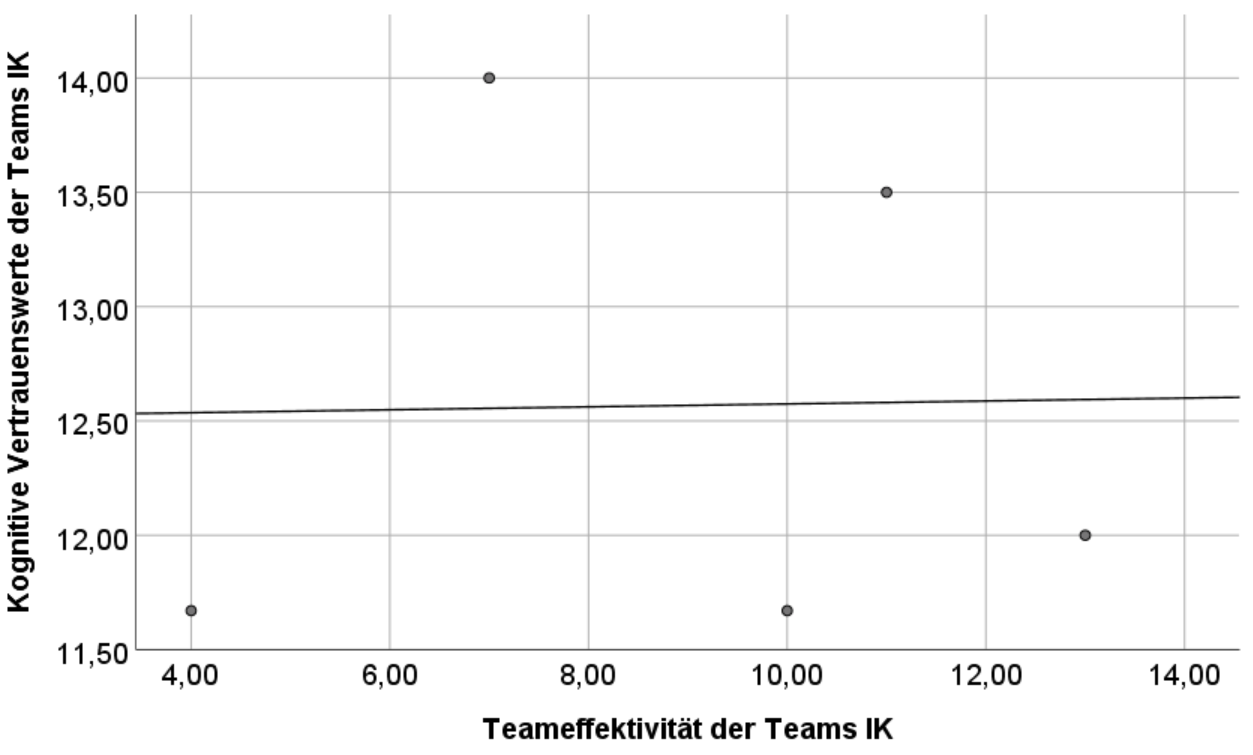
\includegraphics[width=0.45\linewidth]{Abbildungen/AuswertungDiagramme/Final/H_3_Korr_IK.png}}
  \qquad
  \subfloat[][]{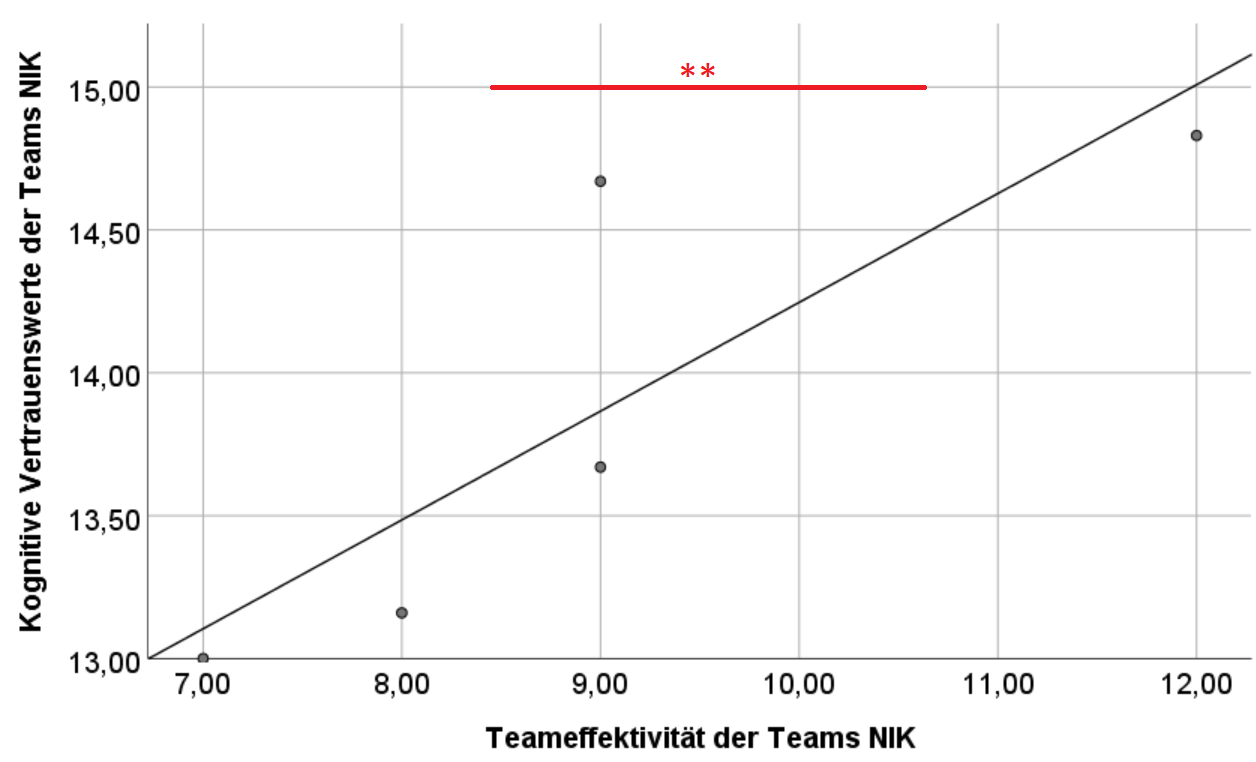
\includegraphics[width=0.45\linewidth]{Abbildungen/AuswertungDiagramme/Final/H_3_Korr_NIK.png}}
  \caption[Korrelationen der kognitiven Vertrauenswerte der Teams mit der Teameffektivität der Teams]{Korrelationen der kognitiven Vertrauenswerte der Teams mit der Teameffektivität der Teams. Links (a) für die Kondition \ac{ik} und rechts (b) für die Kondition \ac{nik}.}
  \label{H3_Korrelation_Auswertung}
\end{figure}

\begin{table}[H]
	\centering\footnotesize\setstretch{1.2}
	\caption[Individuelles kognitives Vertrauen und erfolgreich abgeschlossene Runden]{Die kognitiven Vertrauenswerte und die erfolgreich abgeschlossenen Runden (\textit{Teameffektivität}) - individuell und pro Team zusammengefasst. Kondition 1 definiert die Kondition \ac{ik} und Kondition 2 definiert die Kondition \ac{nik}.}
	\begin{tabularx}{\textwidth}{r | p{2cm} | p{1.5cm} | p{3cm} | p{1.5cm} | p{3cm} } 
		ID & Individueller kognitiver Vertrauenswert & Kondition & Erfolgreich abgeschlossene Runden (Teameffektivität) & Team ID & Summe ind. kog. Vertrauenswerte \\
		\hline 
		1 & $2,50$ & 1 & 4 & Team 1 & $11,67$\\
		2 & $4,67$ & 1 & 4 & &\\
		3 & $4,50$ & 1 & 4 & & \\
		\hline 
		4 & $4,17$ & 1 & 10 & Team 2 & $11,67$\\
		5 & $3,83$ & 1 & 10 & &\\
		6 & $3,67$ & 1 & 10 & &\\
		\hline 
		7 & $5,00$ & 1 & 7 & Team 3 & $14,00$\\
		8 & $4,00$ & 1 & 7 & & \\
		9 & $5,00$ & 1 & 7 & & \\
		\hline 
		10 & $4,50$ & 1 & 11 & Team 4 & $13,50$ \\
		11 & $4,17$ & 1 & 11 & & \\
		12 & $4,83$ & 1 & 11 & & \\
		\hline 
		13 & $4,33$ & 1 & 13 & Team 5 & $12,00$ \\
		14 & $4,17$ & 1 & 13 & & \\
		15 & $3,50$ & 1 & 13 & & \\
		\hline 
		16 & $5,00$ & 2 & 9 & Team 6 & $14,67$ \\
		17 & $4,67$ & 2 & 9 & &\\
		18 & $5,00$ & 2 & 9 & &\\
		\hline 
		19 & $5,00$ & 2 & 12 & Team 7 & $14,83$ \\
		20 & $4,83$ & 2 & 12 & & \\
		21 & $5,00$ & 2 & 12 & & \\
		\hline 
		22 & $4,83$ & 2 & 8 & Team 8 & $13,16$ \\
		23 & $4,33$ & 2 & 8 & & \\
		24 & $4,00$ & 2 & 8 & & \\
		\hline 
		25 & $4,33$ & 2 & 7 & Team 9 & $13,00$ \\
		26 & $4,50$ & 2 & 7 & & \\
		27 & $4,17$ & 2 & 7 & & \\
		\hline 
		28 & $4,67$ & 2 & 9 & Team 10 & $13,67$ \\
		29 & $4,83$ & 2 & 9 & &\\
		30 & $4,17$ & 2 & 9 & & \\	
	\end{tabularx}
	\label{TeamCogTabelle}
\end{table}

\newpage
\subsection{Auswertung Hypothese 4}
\label{Auswertung Hypothese 4}
%H4$_{0}$: Die Mittelwerte der \textit{Teameffektivität} unterscheidet sich bei den Konditionen \ac{ik} und \ac{nik} nicht signifikant voneinander.

\paragraph{Allgemeines}
Auf \textit{Konditionsebene} wird analysiert, ob die Teilnehmer aufgrund unterschiedlicher Avatar-Konditionen eine unterschiedliche \textit{Teameffektivität} besitzen.\\
Die \textit{Teameffektivität} ist laut Shapiro-Wilk-Test ($p =,113 > \alpha = ,05$) normalverteilt. Daher wurde auf Varianzgleichheit der \textit{Teameffektivitätswerte} der unterschiedlichen Avatar-Konditionen geprüft. Der Levene-Test zeigt keine Varianzgleichheit zwischen den \textit{Teameffektivitätswerten} der Kondition \ac{ik} und den \textit{Teameffektivitätswerten} der Kondition \ac{nik} ($L = 10,182; p=,003 < \alpha = ,05$). Dadurch kann davon ausgegangen werden, dass sich die Varianzen \textit{signifikant} voneinander unterscheiden. \\
Die \textit{Teameffektivität} beträgt für die Kondition \ac{ik} im Durchschnitt $\bar{x} = 9,000$ mit einer Standardabweichung von $\sigma = 3,273$.\newline 
Die \textit{Teameffektivität} beträgt für die Kondition \ac{nik} im Durchschnitt $\bar{x} = 9,000$ mit einer Standardabweichung von $\sigma = 1,732$ (siehe \textit{Abbildung \ref{BP_realeTeameffektivität}} und \textit{Abbildung \ref{H4_Mittelwerte_Auswertung}}).

%Aufgrund der Varianzgleichheit hier doch ein Mann-Whitney-U-Test?
%\paragraph{T-Test für unabhängige Stichproben}
%Der T-Wert für unabhängige Stichproben ist kleiner Null ($T = 1,000 > 0$), was auf keinen Mittelwertsunterschied zwischen \ac{tRoundIK} und \ac{tRoundNIK} hinweist. Der Mittelwert $\bar(x) = 9,000$ der Kondition \ac{ik} ist kleiner als der Mittelwert $\bar(x) = 9,000$ der Kondition \ac{nik}.
%Der T-Test für unabhängige Stichproben ergibt bei der Analyse der Differenz des durchschnittlichen \ac{tRound} bei der Kondition \ac{ik} ($\bar(x) = 9,000; \sigma =  3,2732$) und \ac{nik} ($\bar(x) = 9,000; \sigma = 1,7320$) \textbf{keine Signifikanz} ($t(21,270) =,00; p = 1.000 > \alpha = ,05$).

\paragraph{Mann-Whitney-U-Test}
Die Verteilungen der \textit{Teameffektivitätswerte} der Kondition \ac{ik} und der \textit{Teameffektivitätswerte} der Kondition \ac{nik} unterscheiden sich laut Kolmogorov - Smirnov ($p =,181 > \alpha = ,05$) \textbf{nicht signifikant} voneinander. Es gibt \textbf{keinen signifikanten Unterschied} zwischen den Mittelwerten der \textit{Teameffektivität} der Kondition \ac{ik} $(\bar{x} = 9,000$) und der Kondition \ac{nik} $(\bar{x} = 9,000)$ mit $U = 103,500; Z = -,377; p =,706 > \alpha = ,05; r = -,060$. \\

	\begin{figure}[H]
   \begin{minipage}[t]{.5\linewidth} % [b] => Ausrichtung an \caption
      \includegraphics[width=\linewidth]{Abbildungen/AuswertungDiagramme/Final/BP_realeTeameffektivität.png}
      \caption[Boxplot der Teameffektivitätswerte]{Boxplot der Teameffektivitätswerte.}
            \label{BP_realeTeameffektivität}
   \end{minipage}
   \hspace{.02\linewidth}% Abstand zwischen Bilder
   \begin{minipage}[t]{.5\linewidth} % [b] => Ausrichtung an \caption
     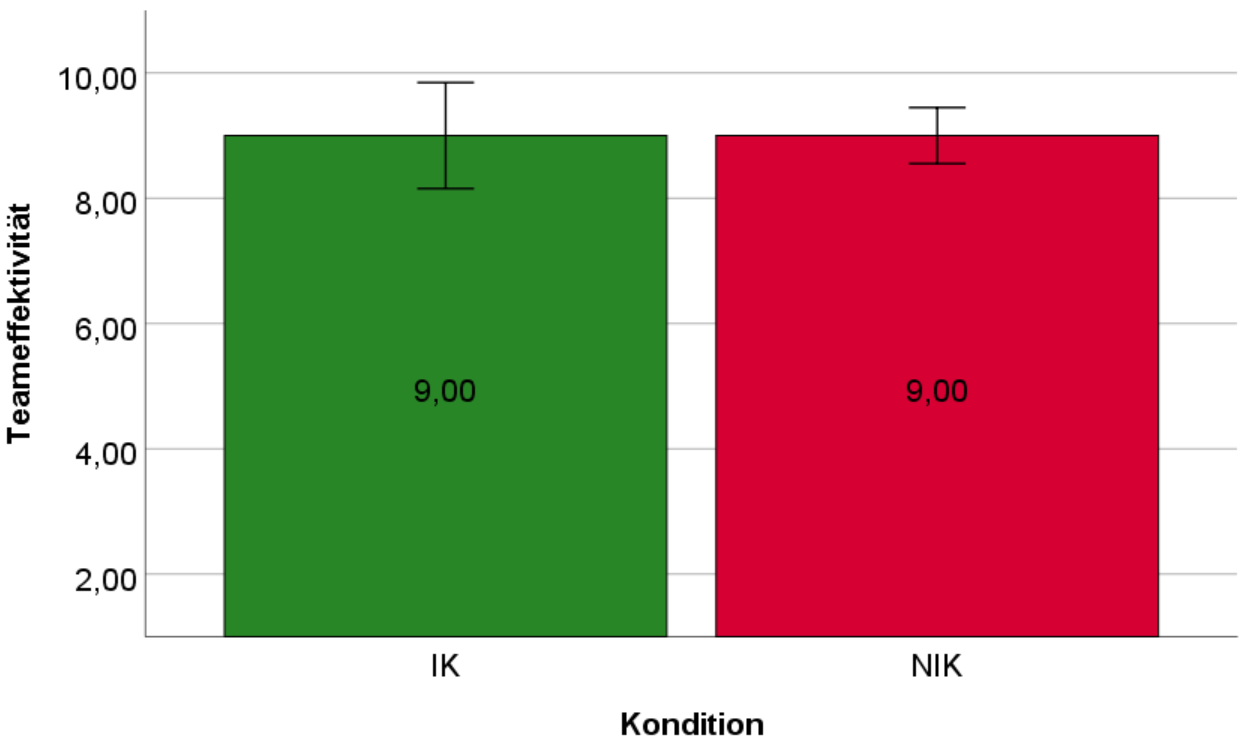
\includegraphics[width=\linewidth]{Abbildungen/AuswertungDiagramme/Final/H4_Mittelwerte.png}
      \caption[Mittelwerte und der Standardfehler der Teameffektivität]{Die durchschnittliche \textit{Teameffektivität} unterschiedlicher Avatar-Konditionen. Die Fehlerbalken zeigen den Standardfehler. Links die Kondition \ac{ik} und rechts die Kondition \ac{nik}.}
       \label{H4_Mittelwerte_Auswertung}
   \end{minipage}
\end{figure}

\newpage
\subsection{Auswertung Hypothese 5}
\label{Auswertung Hypothese 5}
%\textbf{H5$_{0}$} : Der Zusammenhang zwischen dem \textit{generellen Vertrauenswert eines Teams} und der \textit{Teameffektivität eines Teams} mit der Kondition \ac{ik} unterscheidet sich nicht signifikant von den Teams mit der Kondition \ac{nik}. \\
%Besitzt nun Korr. A eine signifikanz und Korr B. nicht, weiss ich, dass die Kondition einen Einfluss auf die anz. abg. Runden besitzt. (Trotzdem sollte ich Fishers-Z-Transformation machen.
%Besitzt nun Korr. A eine signifikanz und Korr B. auch, kann ich schauen, ob diese sich signifikant unterscheiden. (Ich MUSS eine Fisher-Z-Transformation machen)
%Besitzt nun Korr. A keine signifikanz und Korr B. auch nicht, hat der generelle Trust Score keine Auswirkung auf die anz. abgeschlossenen Runden und es ist egal welche Kondition ich laut dieser Hypothese nehme. ( Ich müsste keine Fisher-Z-Transformation machen)
\paragraph{Allgemeines}
Es wird der Zusammenhang zwischen dem \textit{generellen Vertrauenswert von Teams} und der \textit{Teameffektivität von Teams} auf Teamebene analysiert.
 
\paragraph{Vertrauenstabelle pro Team}
Es wird der \textit{generelle Vertrauenswert eines Teams} durch das Aufsummieren der individuellen \textit{generellen Vertrauenswerte} der drei Personen eines Teams gebildet.
Da jedes Teammitglied dieselbe Anzahl an Runden abgeschlossen hat, besitzen diese drei Teammitglieder dieselbe \textit{Teameffektivität}.
Es wird eine Spearman-Korrelation zwischen der \textit{Teameffektivität der Teams} und den \textit{generellen Vertrauenswerten der Teams} pro Avatar-Kondition durchgeführt, um Zusammenhänge untereinander festzustellen zu können.
Damit überprüft werden kann, ob sich die beiden Spearman-Korrelationen signifikant voneinander unterscheiden, wird anschließend eine Fisher-Z-Transformation für unabhängige Stichproben durchgeführt. Die individuellen generellen Vertrauenswerte und die erfolgreich abgeschlossenen Runden (\textit{Teameffektivität}) sind in der \textit{Tabelle \ref{TeamGenTabelle}} dargestellt:\\
Die \textit{generellen Vertrauenswerte der Teams} mit der Kondition \ac{ik} sind laut Shapiro-Wilk-Test mit $p =,210 > \alpha = ,05$ normalverteilt. \newline
Die \textit{generellen Vertrauenswerte der Teams} mit der Kondition \ac{nik} sind laut Shapiro-Wilk-Test mit $p =,091 > \alpha = ,05$ normalverteilt. \newline
Die \textit{Teameffektivitätswerte der Teams} mit der Kondition \ac{ik} sind laut Shapiro-Wilk-Test mit $p =,844 > \alpha = ,05$ normalverteilt. \newline
Die \textit{Teameffektivitätswerte der Teams} mit der Kondition \ac{nik} sind laut Shapiro-Wilk-Test mit $p =,453 > \alpha = ,05$ normalverteilt. \\
Das Lowess-Verfahren deutet augenscheinlich auf keinen linearen Zusammenhang zwischen den \textit{generellen Vertrauenswerten der Teams} mit der Kondition \ac{ik} und den \textit{Teameffektivitätswerten der Teams} mit der Kondition \ac{ik} sowie auf keinen linearen Zusammenhang zwischen den \textit{generellen Vertrauenswerten der Teams} mit der Kondition \ac{nik} und den \textit{Teameffektivitätswerten der Teams} mit der Kondition \ac{nik} hin. Daher wird die Linearitätsannahme nicht angenommen.\\
Aufgrund des geringen Stichprobenumfangs der Teams pro Avatar-Kondition ($N=5$) und der nicht eindeutigen Linearität durch das Lowess-Verfahren, wurde sich für eine Spearman-Korrelation entschieden.

\paragraph{Spearman-Korrelation}
Es ist eine starke negative Korrelation (vgl. \citep{cohen2013statistical}) mit dem Spearman-Korrelationskoeffizient $r = -,800$ zwischen den \textit{generellen Vertrauenswerten der Teams} mit der Kondition \ac{ik} und den \textit{Teameffektivitätswerten der Teams} mit der Kondition \newline \ac{ik} vorhanden. Die Spearman-Korrelation ist \textbf{nicht signifikant} ($p =,104 > \alpha = ,05$).\\
Weiterhin ist eine starke negative Korrelation (vgl. \citep{cohen2013statistical}) mit dem Spearman- Korrelationskoeffizient $r = -,667$ zwischen den \textit{generellen Vertrauenswerten der Teams} mit der Kondition \ac{nik} und den \textit{Teameffektivitätswerten der Teams} mit der Kondition \newline \ac{nik} vorhanden. Die Spearman-Korrelation ist \textbf{nicht signifikant} ($p =,219 > \alpha = ,05$) (siehe \textit{Abbildung \ref{H5_Korrelation_Auswertung}}). 

\paragraph{Fisher-Z-Transformation für unabhängige Stichproben}
Es wird eine Fisher-Z-Transformation für unabhängige Stichproben durchgeführt.
Die beiden Spearman-Korrelationen unterscheiden sich laut Fisher-Z-Wert für unabhängige Stichproben ($Z=-,293$) \textbf{nicht signifikant} voneinander ($p =,385 > \alpha = ,05$).

\begin{figure}[h]
  \centering
  \subfloat[][]{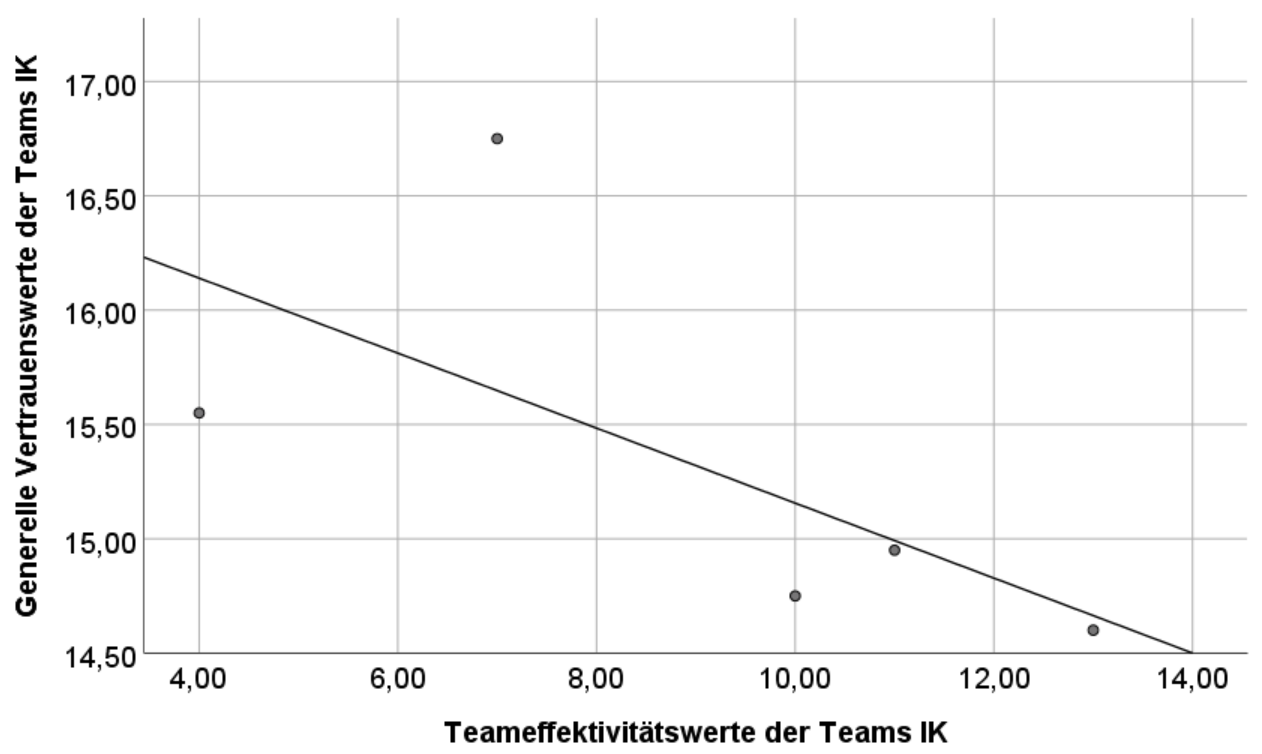
\includegraphics[width=0.45\linewidth]{Abbildungen/AuswertungDiagramme/Final/H_5_Korr_IK.png}}
  \qquad
  \subfloat[][]{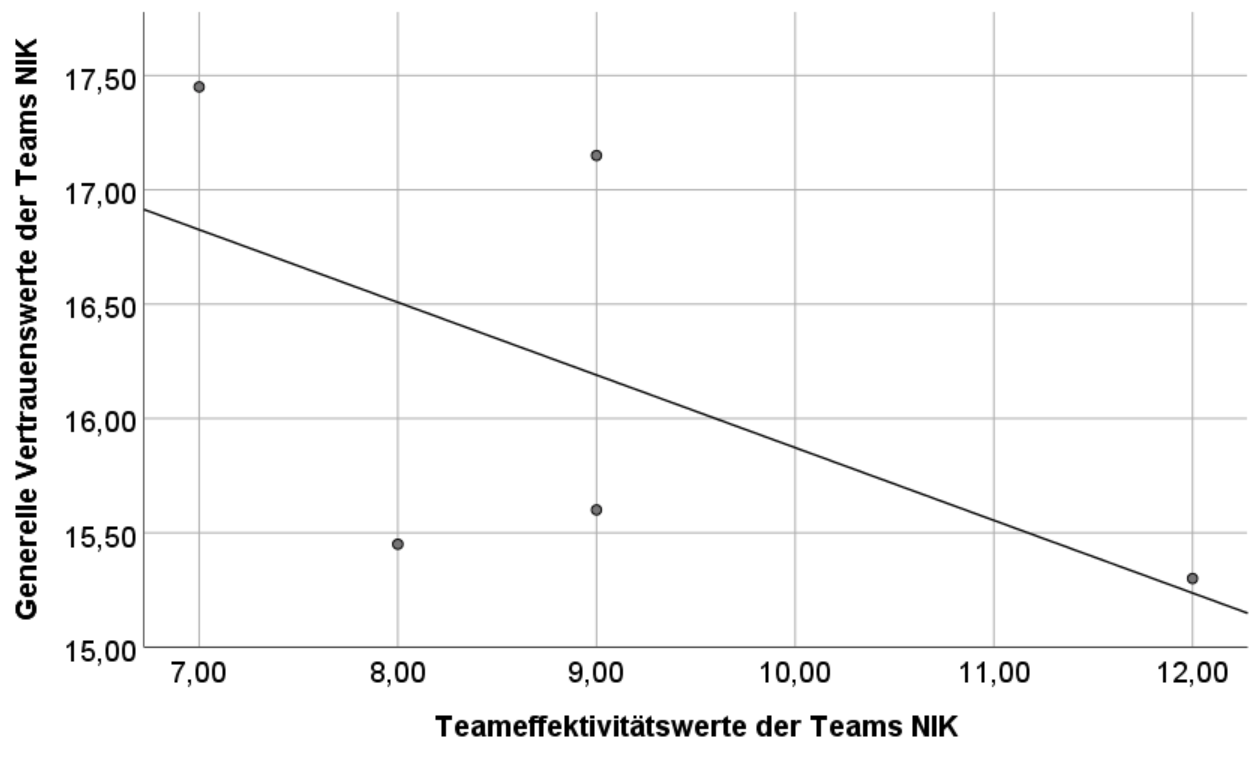
\includegraphics[width=0.45\linewidth]{Abbildungen/AuswertungDiagramme/Final/H_5_Korr_NIK.png}}
  \caption[Korrelationen der generellen Vertrauenswerte der Teams mit der Teameffektivität der Teams]{Korrelationen der generellen Vertrauenswerte der Teams mit der Teameffektivität der Teams. Links (a) für die Kondition \ac{ik} und rechts (b) für die Kondition \ac{nik}.}
  \label{H5_Korrelation_Auswertung}
\end{figure}

\begin{table}[H]
	\centering\footnotesize\setstretch{1.2}
		\caption[Individuelles generelles Vertrauen und erfolgreich abgeschlossene Runden]{Die individuellen generellen Vertrauenswerte und die erfolgreich abgeschlossenen Runden (\textit{Teameffektivität}) - individuell und pro Team zusammengefasst. Kondition 1 definiert die Kondition \ac{ik} und Kondition 2 definiert die Kondition \ac{nik}.}
	\begin{tabularx}{\textwidth}{r | p{2cm} p{1.5cm} p{3cm} p{1.5cm} p{1.5cm} p{1.5cm} p{1.5cm}} 
		ID & Individueller genereller Vertrauenswert & Kondition & Erfolgreich abgeschlossene Runden (Teameffekvitität) & Team ID & Summe ind. gen. Vertrauenswerte\\
		\hline 
		1 & $5,35$ & 1 & 4 & Team 1 & $15,55$\\
		2 & $4,70$ & 1 & 4 & &\\
		3 & $5,50$ & 1 & 4 & & \\
		\hline 
		4 & $5,60$ & 1 & 10 & Team 2 & $14,75$\\
		5 & $3,60$ & 1 & 10 & &\\
		6 & $5,55$ & 1 & 10 & &\\
		\hline 
		7 & $6,10$ & 1 & 7 & Team 3 & $16,75$\\
		8 & $5,00$ & 1 & 7 & & \\
		9 & $5,65$ & 1 & 7 & & \\
		\hline 
		10 & $5,55$ & 1 & 11 & Team 4 & $14,95$ \\
		11 & $4,40$ & 1 & 11 & & \\
		12 & $5,00$ & 1 & 11 & & \\
		\hline 
		13 & $5,10$ & 1 & 13 & Team 5 & $14,60$ \\
		14 & $5,05$ & 1 & 13 & & \\
		15 & $4,45$ & 1 & 13 & & \\
		\hline 
		16 & $6,00$ & 2 & 9 & Team 6 & $17,15$ \\
		17 & $5,45$ & 2 & 9 & &\\
		18 & $5,70$ & 2 & 9 & &\\
		\hline 
		19 & $4,90$ & 2 & 12 & Team 7 & $15,30$ \\
		20 & $5,00$ & 2 & 12 & & \\
		21 & $5,40$ & 2 & 12 & & \\
		\hline 
		22 & $5,35$ & 2 & 8 & Team 8 & $15,45$ \\
		23 & $4,60$ & 2 & 8 & & \\
		24 & $5,50$ & 2 & 8 & & \\
		\hline 
		25 & $4,90$ & 2 & 7 & Team 9 & $17,45$ \\
		26 & $6,15$ & 2 & 7 & & \\
		27 & $6,40$ & 2 & 7 & & \\
		\hline 
		28 & $6,00$ & 2 & 9 & Team 10 & $15,60$ \\
		29 & $5,20$ & 2 & 9 & &\\
		30 & $4,40$ & 2 & 9 & & \\	
	\end{tabularx}
	\label{TeamGenTabelle}
\end{table}

\begin{table}[H]
	\centering\footnotesize\setstretch{1}
	\caption[Übersicht zur Auswertung der Hypothesen 1 - 3]{Übersicht zur Auswertung der Hypothesen 1 - 3}
	\label{VariableBreakdown1}
	\begin{tabularx}{\textwidth}{| p{3cm} | p{2.75cm} | p{3.5cm} | p{4cm} |} 
		\hline Was wurde gemessen? & Hypothese 1 & Hypothese 2 & Hypothese 3 \\
		\hline
		Shapiro-Wilk-Test
		&
		$\textit{kognitives Vertrauen}:$\newline\fbox{$p=,002<\alpha=,05^*$} \newline		
		& 
		$\textit{generelles Vertrauen - IK}:$\newline$p=,382>\alpha=,05$\newline 
		$\textit{generelles Vertrauen - NIK}:$\newline $p=,944>\alpha=,05$ \newline
		$\textit{kognitives Vertrauen - IK}:$\newline$p=,183>\alpha=,05$ \newline 
		$\textit{kognitives Vertrauen - NIK}:$\newline$p=,069>\alpha=,05$ \newline
		& 
		$\textit{kognitives Vertrauen Team - IK}:$\newline $p=,109>\alpha=,05$ \newline 
		$\textit{kognitives Vertrauen Team - NIK}:$\newline $p=,278>\alpha=,05$ \newline
		$\textit{Teameffektivität - IK}:$\newline $p=,844>\alpha=,05$ \newline 
		$\textit{Teameffektivität - NIK}:$\newline $p=,453>\alpha=,05$ \\ 

		\hline 		
		
		Mann-Whitney-U 
		& 
		\textit{Kolm. Smirnov}:\newline$p=,925>\alpha=,05$ \newline
		\textit{Mann-Whitney-U} :\newline
		$U=64,000$\newline $Z=-2,029$ \newline 
		\fbox{$p=,042<\alpha=,05^*$} \newline 
		$r=-,370$
		& 
		&  \\
		
		\hline 				
	
		Spearman-Roh Korrelation 
		&
		& $\textit{generelles Vertrauen - IK}$ und \newline $\textit{kognitives Vertrauen - IK}:$\newline
		$r=,406$\newline
		$p=,134>\alpha=,05$\newline ------------------------------------ \newline
		$\textit{generelles Vertrauen - NIK}$ und $\textit{kognitives Vertrauen - NIK}:$\newline
		$r=,045$\newline
		$p=,872>\alpha=,05$\newline
		& $\textit{kognitives Vertrauen Team - IK}$ und $\textit{Teameffektivität - IK}:$\newline
		$r=,205$\newline$p=,741>\alpha=,05$\newline ------------------------------------ \newline
		$\textit{kognitives Vertrauen Team - NIK}$ und $\textit{Teameffektivität - NIK}:$\newline
		$r=,975$\newline
		\fbox{$p=,005<\alpha=,05^*$} \\
		
		\hline 		
		
		Fishers-Z-Transformation für unabh. Stichp.
		&
		&  $\textit{r=,406; N=5}$ und $\textit{r=,045; N=5} :$\newline \newline
		$Z=,954$\newline
		\fbox{$p=,017<\alpha=,05^*$}
		& $\textit{r=,205; N=5}$ und $\textit{r=,975; N=5} :$\newline \newline
		$Z=-1,977$\newline
		\fbox{$p=,024<\alpha=,05^*$} \\
		
		\hline 
	\end{tabularx}
\end{table}		

\begin{table}[H]
	\centering\footnotesize\setstretch{1}
	\caption[Übersicht zur Auswertung der Hypothesen 4 - 5]{Übersicht zur Auswertung der Hypothesen 4 - 5}
	\label{VariableBreakdown2}
	\begin{tabularx}{\textwidth}{| p{3.7cm} | p{5cm} | p{5cm} |} 
		\hline Was wurde gemessen? & Hypothese 4 & Hypothese 5  \\
		\hline
		Shapiro-Wilk-Test
		&
		$\textit{Teameffektivität}:$\newline$p=,113>\alpha=,05$\newline 
		& 
		$\textit{kognitives Vertrauen Team - IK}:$\newline$p=,210>\alpha=,05$\newline 
		$\textit{kognitives Vertrauen Team - NIK}:$\newline$p=,091>\alpha=,05$\newline 
		$\textit{Teameffektivität - IK}:$\newline$p=,844>\alpha=,05$\newline 
		$\textit{Teameffektivität - NIK}:$\newline$p=,453>\alpha=,05$\\ 
	
		\hline 

		Mann-Whitney-U 
		&
		\textit{Kolm. Smirnov}:\newline$p=,181>\alpha=,05$\newline
		\textit{Mann-Whitney-U}:\newline
		$U=103,500$\newline 
		$Z=-,377$ \newline 
		$p=-,706>\alpha=,05$ \newline 
		$r=-,060$
		& 

		\\
		\hline 				
		
		Varianzgleichheit
		&  \textit{Levene-Test}: \newline \fbox{$L=10,182$\newline$p=,003<\alpha=,05^*$} \newline
		& \\

		\hline 		

		Spearman-Roh Korrelation 
		&
		&$\textit{generelles Vertrauen Team - IK}$ und \newline $\textit{Teameffektivität - IK}$:\newline
		$r=-,800$\newline
		$p=,104>\alpha=,05$\newline ------------------------------------ \newline
		$\textit{generelles Vertrauen Team -NIK}$ und $\textit{Teameffektivität - NIK}$:\newline
		$r=-,667$\newline
		$p=,219>\alpha=,05$ \\
		
		\hline 		

		Fishers-Z-Transformation für unabh. Stichp.
		&
		& $\textit{r=-,800; N=5}$ und $\textit{r=-,667; N=5} :$\newline \newline
		$Z=-,293$\newline
		$p=,385>\alpha=,05$ \\
		
		\hline 	
	\end{tabularx}
\end{table}		

%In der folgenden Tabelle wird beschrieben, ob die einzelnen Hypothesen Signifikanz aufweisen.

%\subsection{Analyse Hypothese 7}
%

% WO IST MEHR WAHRGENOMENE TEAMEFFEKTIVITÄT VORHANDEN??

%Unterschiedliche wahrgenommene \textit{Teameffektivität} bei unterschiedlichen Avatar-Konditionen.

%Auch interessant : T-Test zwischen COPRÄSENZ und WieSahenIhreMitspielerAus
%
%Auch interessant : Wie wirkt sich gt und CT gemeinsam auf TE aus? ( Auch im Team )
%
%Auch interssant : Rounds Done im Verhältnis zu Team-Effectiveness-Scale
%Auch interessant : Wie ist das Verhältnis von gedachtem Effektivitätswert zu eigentlichem tRounds?
%
%
%Auch interessant : NASA-TLX( WIE ANSTRENGEND WAR ES?) zur Round-Efficiency
%
%Auch interessant : T-Test von Team-Communication bei den IK und NON IK Gruppen
%	Hier signifikanten unterschied der Mittelwerte gefunden!
%	
%Auch interessant : Team-Communication zur Rounds Done


%AUch interessant :   Schlechte Teams sollten auch ein schlechteres Cognitives Vertrauen besitzen! Ist das der Fall??

%-------------------------------------------------------------------------------
% WAR MEHR PRÄSENZ BEI IK ODER NIK AVATAR VORHANDEN?
%KAPITEL : VR - Präsenz in Virtual Reality

%KAPITEL : Vertrauen als Zustand - Kognitives und Affektives Vertrauen
%Ich glaube, ich habe die Aufgaben des Versuchsleiters gut erledigt -> Auf Kognitives Vertrauen analisieren Pro person! Hier ist einseitige Signifikanz in der Korrelation von Wie Erfolgreich haben Sie ihrer Meinung nach die vom Versuchleiter ... mit Cog_Trust_Windsorizing vorhanden!

% Self-Avatare

%Jedoch wurde ein größeres Gefühl von Zusammenheit festgestellt, wenn mit einem Menschenähnlichem Avatar interagiert wurde. \citep{kerr1983motivation}
%Dies auch evenntl überprüfen?
\newpage
\subsection{Auswertung subjektiver Daten}
Im Folgenden werden die subjektiven Fragebögen in Bezug auf die beiden Avatar-Konditionen ausgewertet.

Die subjektiven Daten wurden auf Extremwerte überprüft. Jedoch lassen sich diese Extremwerte nicht pauschal als Ausreißer klassifizieren. Dies geht aus dem jeweiligen Feedback der Nutzer hervor sowie dem Vergleich anderer angegebener Werte der Fragebögen. Die milden Extremwerte der \textit{Präsenz}, der \textit{Telepräsenz} sowie der \textit{wahrgenommenen Co-Präsenz des anderen} wurden als plausibel eingestuft. 
Der starke Extremwert der \textit{wahrgenommenen Teameffektivität} (ID1) wurde ebenfalls als plausibel eingestuft, da dieser Teilnehmer zum Team mit der schlechtesten Teameffektivität gehörte. Aus diesem Grund wird dieser Extremwert nicht verworfen.
In \textit{Tabelle \ref{SubSigTab}} befindet sich eine Übersicht, ob es signifikante Unterschiede zwischen den Avatar-Konditionen bei den erhobenen subjektiven Daten gibt.

\paragraph{Präsenz}
Das Gefühl der \textit{Präsenz} ist laut Shapiro-Wilk-Test mit $p =,077 > \alpha = ,05$ normalverteilt. 
Dies beträgt bei der Kondition \ac{ik} im Durchschnitt $\bar{x} = 4,423$ mit einer Standardabweichung von $\sigma = 1,024$.
Bei der Kondition \ac{nik} beträgt dies im Durchschnitt $\bar{x} = 4,504$ mit einer Standardabweichung von $\sigma =,926$.
Der T-Test für unabhängige Stichproben zeigt \textbf{keine signifikanten Unterschiede} zwischen den Mittelwerten ($t(28) = -,227; p =,822 > \alpha = ,05$) (siehe \textit{Abbildung \ref{SD_PresenceBP}} und \textit{Abbildung \ref{SD_Presence_Mittel}}).

\begin{figure}[H]
   \begin{minipage}[t]{.5\linewidth} % [b] => Ausrichtung an \caption
      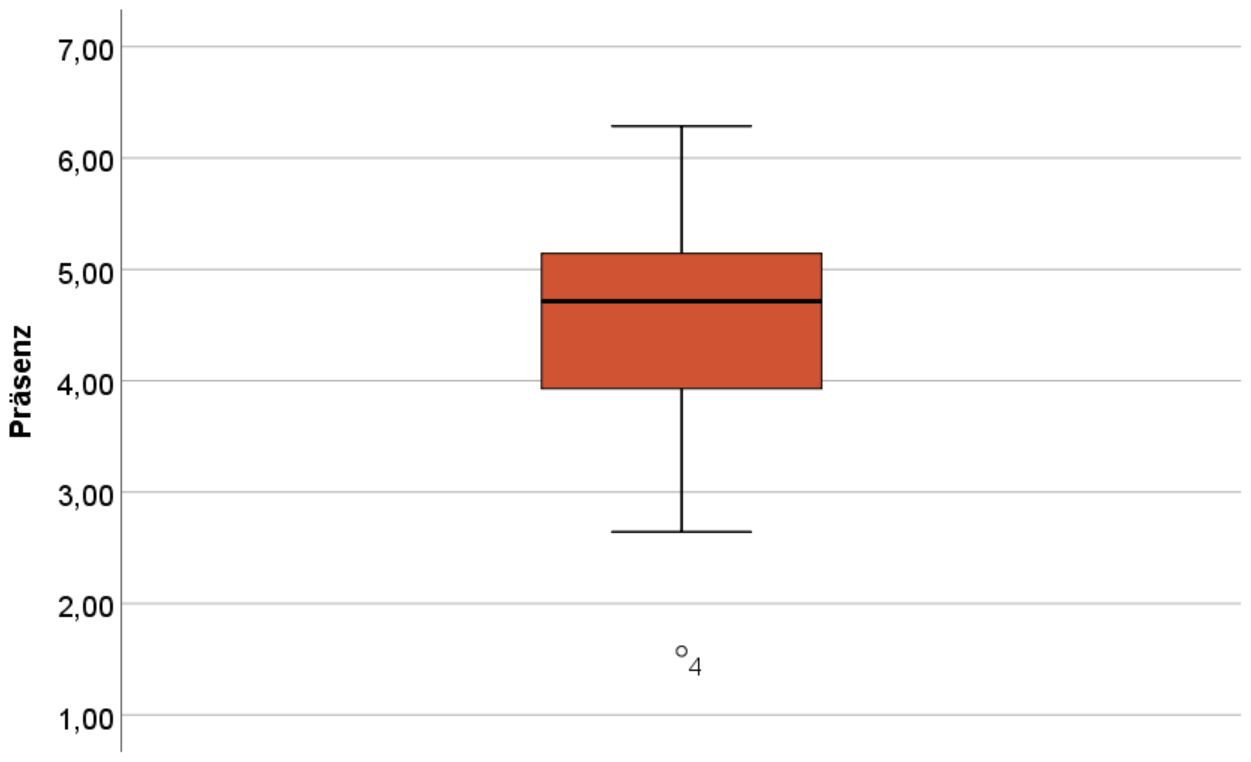
\includegraphics[width=\linewidth]{Abbildungen/AuswertungDiagramme/Final/BP_Presence.png}
      \caption[Boxplot der wahrgenommenen Präsenz]{Boxplot der wahrgenommenen Präsenz.}
      \label{SD_PresenceBP}
   \end{minipage}
   \hspace{.02\linewidth}% Abstand zwischen Bilder
   \begin{minipage}[t]{.5\linewidth} % [b] => Ausrichtung an \caption
     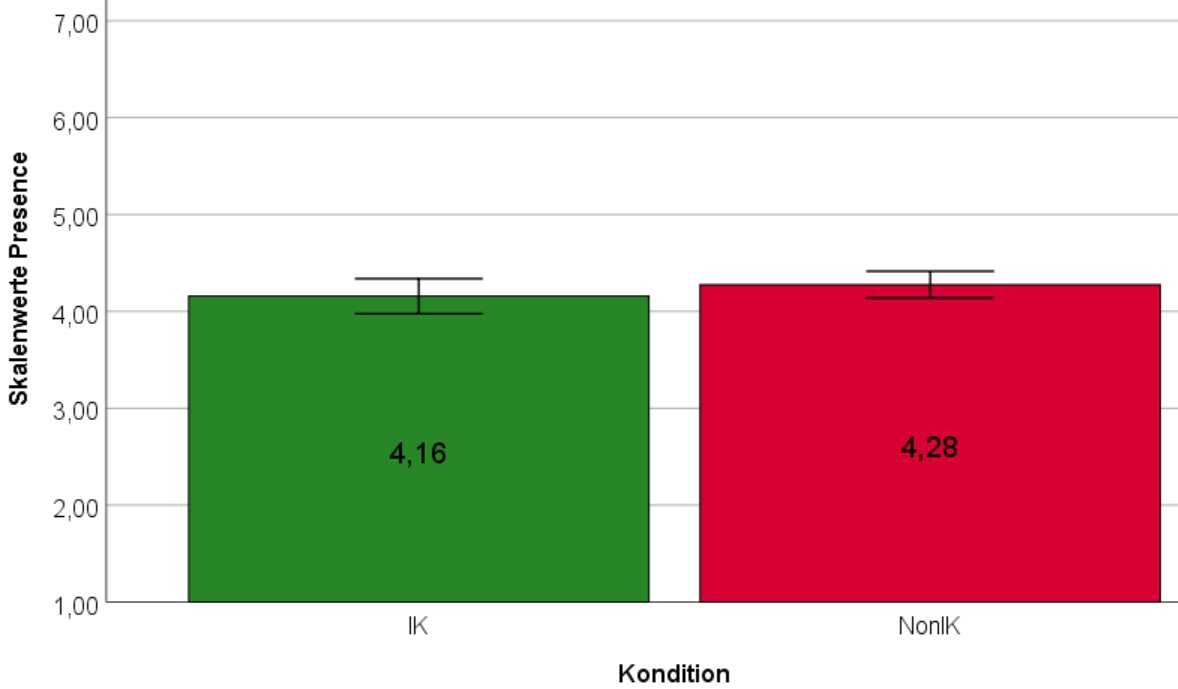
\includegraphics[width=\linewidth]{Abbildungen/AuswertungDiagramme/Final/SD_Presence_Mittelwerte.png}
      \caption[Durchschnittlich wahrgenommene Präsenz der Konditionen]{Die durchschnittlich wahrgenommene Präsenz. Der vertikale Fehler beschreibt den Standardfehler.}
       \label{SD_Presence_Mittel}
   \end{minipage}
\end{figure}

\newpage

\paragraph{Selbst wahrgenommene Co-Präsenz}
Die \textit{selbst wahrgenommene Co-Präsenz} ist laut Shapiro-Wilk-Test mit $p =,009 < \alpha = ,05$ nicht normalverteilt.
Sie beträgt bei der Kondition \ac{ik} im Durchschnitt $\bar{x} = 3,888$ mit einer Standardabweichung von $\sigma =,950$.
Bei der Kondition \newline \ac{nik} liegt das arithmetische Mittel bei $\bar{x} = 3,766$ mit einer Standardabweichung von $\sigma =,959$. 
Laut Mann-Whitney-U-Test gibt es \textbf{keinen signifikanten Unterschied} zwischen den Mittelwerten ($U = 100,500; Z = -,501; p =,617 > \alpha = ,05$) (siehe \textit{Abbildung \ref{SD_SelfCoPresenceBP}} und \textit{Abbildung \ref{SD_SelbstCoPresence_Mittelwerte}}).
	
	\begin{figure}[H]
   \begin{minipage}[t]{.5\linewidth} % [b] => Ausrichtung an \caption
      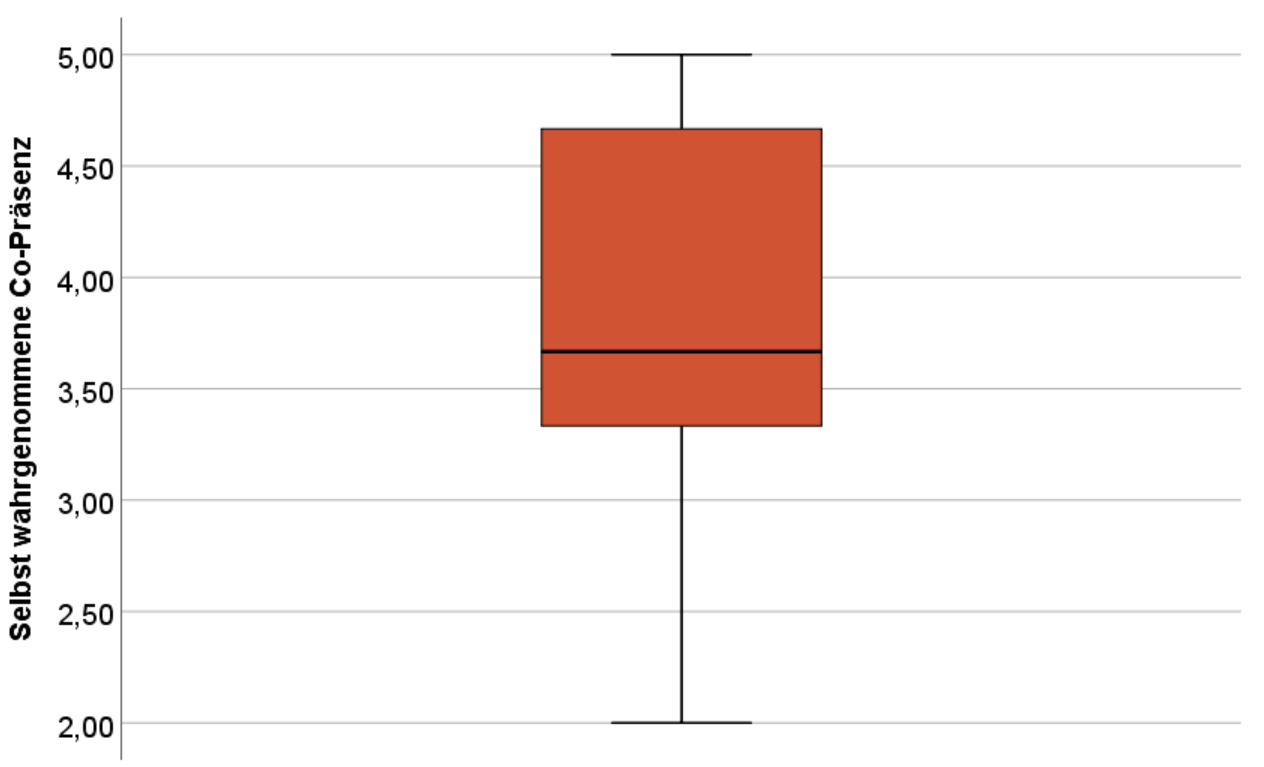
\includegraphics[width=\linewidth]{Abbildungen/AuswertungDiagramme/Final/BP_SelfCoPresence.png}
      \caption[Boxplot der selbst wahrgenommenen Co-Präsenz]{Boxplot der selbst \textit{wahrgenommenen Co-Präsenz}.}
            \label{SD_SelfCoPresenceBP}
   \end{minipage}
   \hspace{.02\linewidth}% Abstand zwischen Bilder
   \begin{minipage}[t]{.5\linewidth} % [b] => Ausrichtung an \caption
     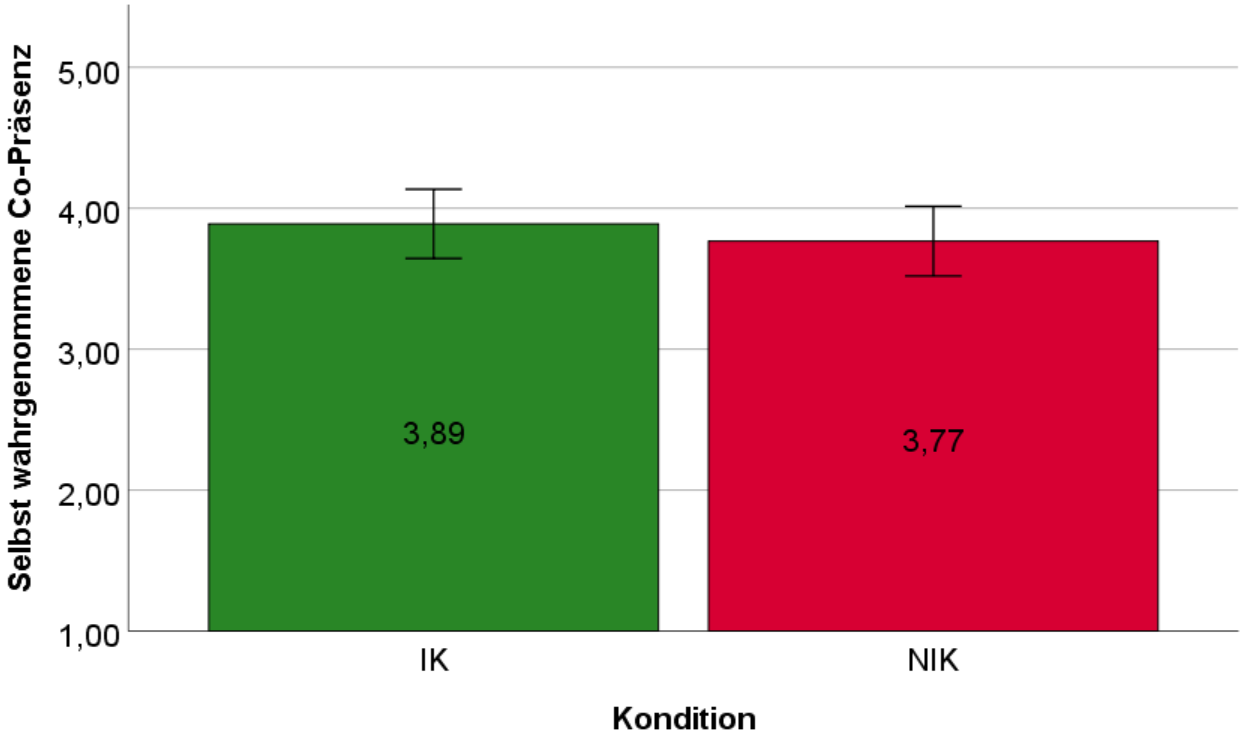
\includegraphics[width=\linewidth]{Abbildungen/AuswertungDiagramme/Final/SD_SelbstCoPresence_Mittelwerte.png}
      \caption[Durchschnittlich selbst wahrgenommene Co-Präsenz der Konditionen]{Diese Abbildung zeigt die durchschnittliche selbst \textit{wahrgenommene Co-Präsenz} der unterschiedlichen Konditionen. Der vertikale Fehler beschreibt den Standardfehler.}
       \label{SD_SelbstCoPresence_Mittelwerte}
   \end{minipage}
\end{figure}

\paragraph{Wahrgenommene Co-Präsenz des anderen}
Die \textit{wahrgenommene Co-Präsenz des anderen} ist laut Shapiro-Wilk-Test mit $p =,101 > \alpha = ,05$ normalverteilt.
Diese beträgt bei der Kondition \ac{ik} im Durchschnitt $\bar{x} = 4,011$ mit einer Standardabweichung von $\sigma =,510$.
Bei der Kondition \ac{nik} beträgt diese im Durchschnitt $\bar{x} = 3,744$ mit einer Standardabweichung von $\sigma = ,730$. 
Der T-Test für unabhängige Stichproben zeigt \textbf{keine signifikanten Unterschiede} zwischen den Mittelwerten ($t(28) = 1,159; p =,256 > \alpha = ,05$) (siehe \textit{Abbildung \ref{SD_OtherCoPresenceBP}} und \textit{Abbildung \ref{SD_SelbstCoPresence_Mittelwerte}}).

	\begin{figure}[H]
   \begin{minipage}[t]{.5\linewidth} % [b] => Ausrichtung an \caption
      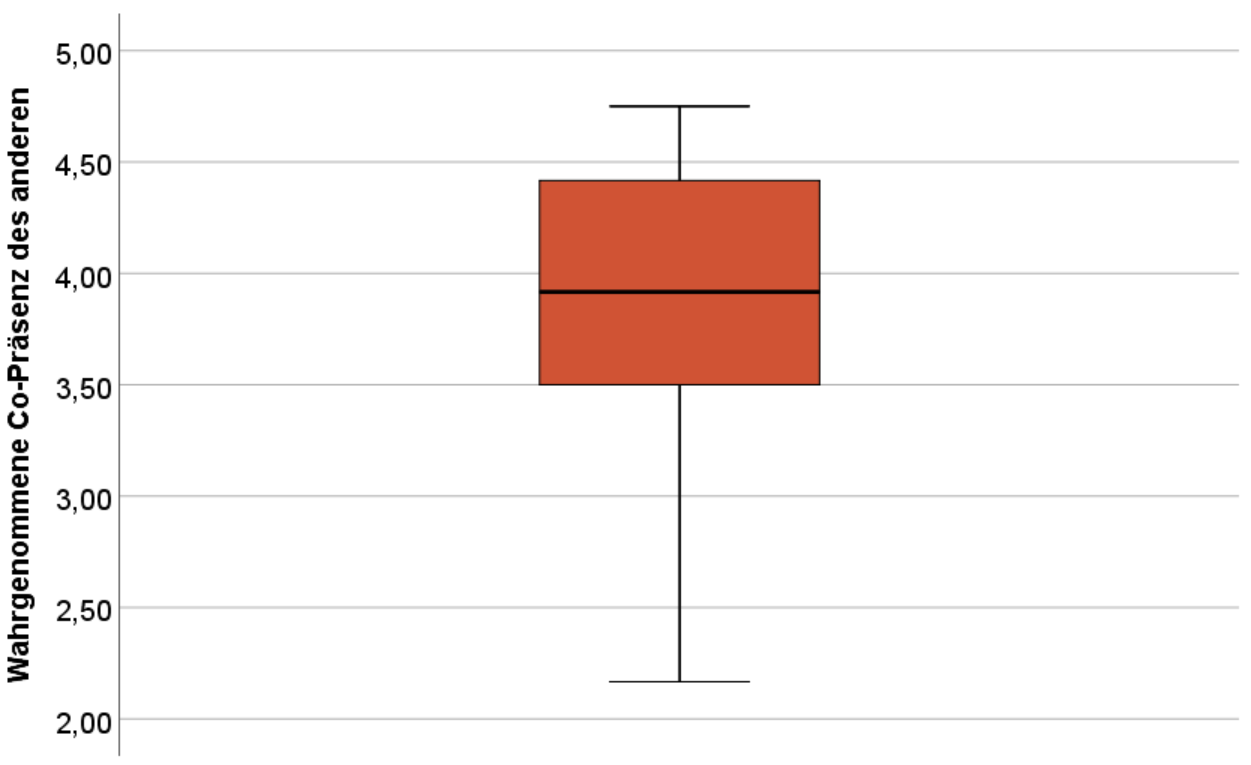
\includegraphics[width=\linewidth]{Abbildungen/AuswertungDiagramme/Final/BP_OtherCoPresence.png}
      \caption[Boxplot der selbst wahrgenommenen Co-Präsenz des anderen]{Diese Abbildung zeigt den Boxplot der \textit{wahrgenommenen Co-Präsenz des anderen}.}
            \label{SD_OtherCoPresenceBP}
   \end{minipage}
   \hspace{.02\linewidth}% Abstand zwischen Bilder
   \begin{minipage}[t]{.5\linewidth} % [b] => Ausrichtung an \caption
     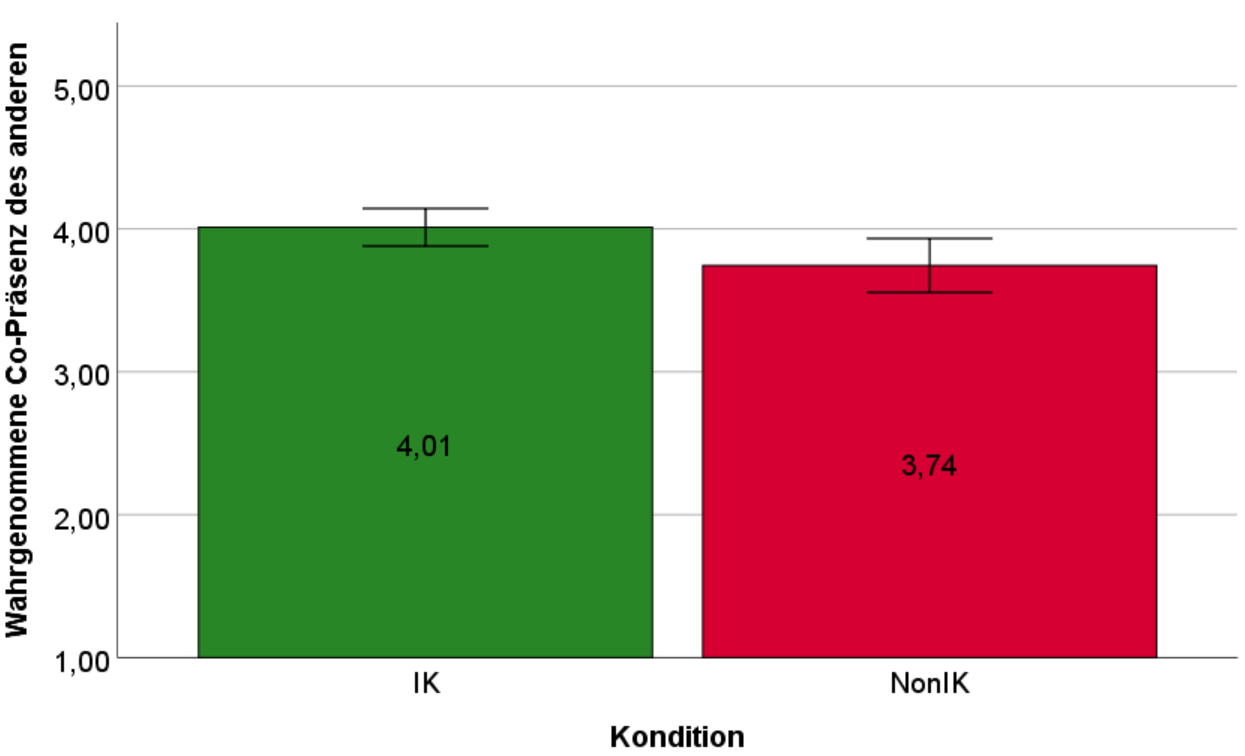
\includegraphics[width=\linewidth]{Abbildungen/AuswertungDiagramme/Final/SD_OtherCoPresence_Mittelwerte.png}
      \caption[Durchschnittliche wahrgenommene Co-Präsenz des anderen der Konditionen]{In dieser Abbildung werden die Mittelwerte der \textit{wahrgenommenen Co-Präsenz des anderen} der unterschiedlichen Konditionen dargestellt. Der vertikale Fehler beschreibt den Standardfehler.}
       \label{SD_SelbstCoPresence_Mittelwerte}
   \end{minipage}
\end{figure}

\newpage

\paragraph{Telepräsenz} 
Die \textit{Telepräsenz} ist laut Shapiro-Wilk-Test mit $p =,024 < \alpha = ,05$ nicht normalverteilt. 
Sie beträgt bei der Kondition \ac{ik} im Durchschnitt $\bar{x} = 5,213$ mit einer Standardabweichung von $\sigma = 1,265$.
Weiterhin beträgt die Telepräsenz bei der Kondition \ac{nik} im Mittel $\bar{x} = 5,360$ mit einer Standardabweichung von $\sigma =,797$. 
Laut Mann-Whitney-U-Test gab es \textbf{keinen signifikanten Unterschied} zwischen den Mittelwerten ($U = 112,000; Z = -,021; p =,983 > \alpha = ,05$) (siehe \textit{Abbildung \ref{SD_Telepresence}} und \textit{Abbildung \ref{SD_Telepresence_Mittelwerte}}).

	\begin{figure}[H]
   \begin{minipage}[t]{.5\linewidth} % [b] => Ausrichtung an \caption
      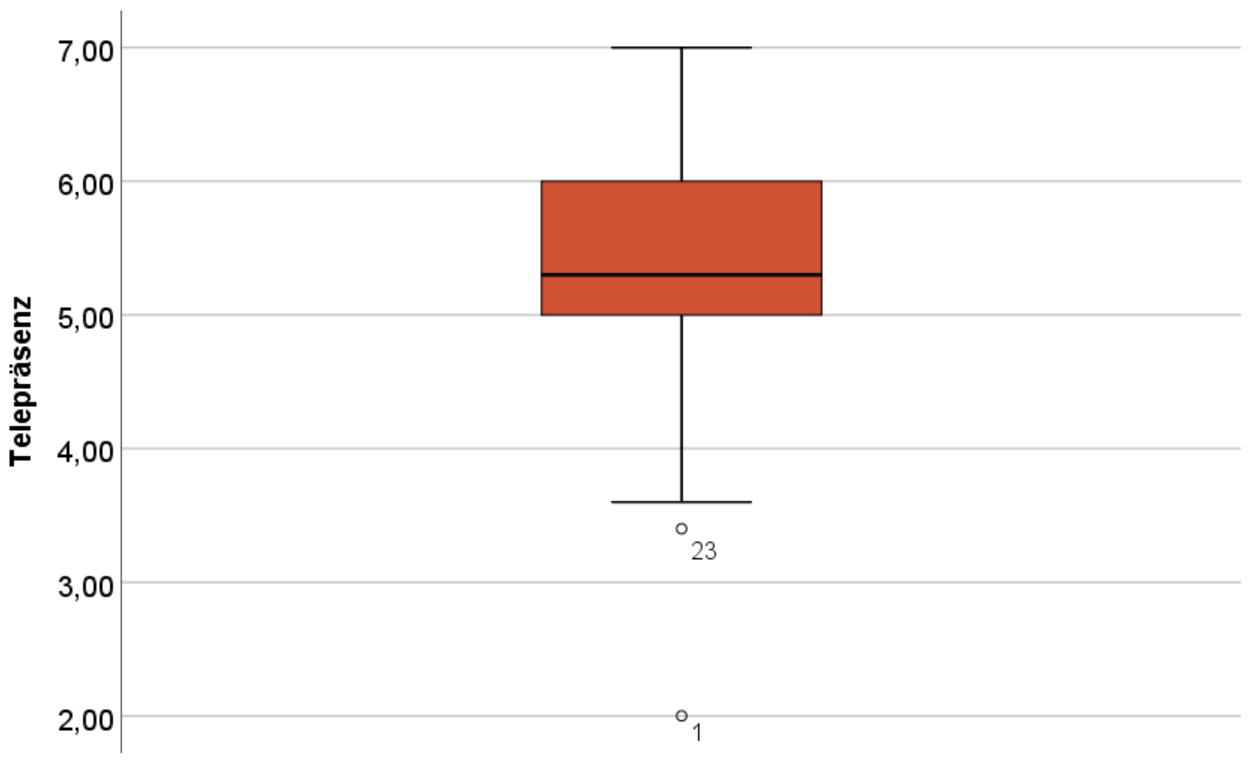
\includegraphics[width=\linewidth]{Abbildungen/AuswertungDiagramme/Final/BP_Telepresence.png}
      \caption[Boxplot der wahrgenommenen Telepräsenz]{Diese Abbildung zeigt den Boxplot der \textit{wahrgenommenen Telepräsenz}.}
            \label{SD_Telepresence}
   \end{minipage}
   \hspace{.02\linewidth}% Abstand zwischen Bilder
   \begin{minipage}[t]{.5\linewidth} % [b] => Ausrichtung an \caption
     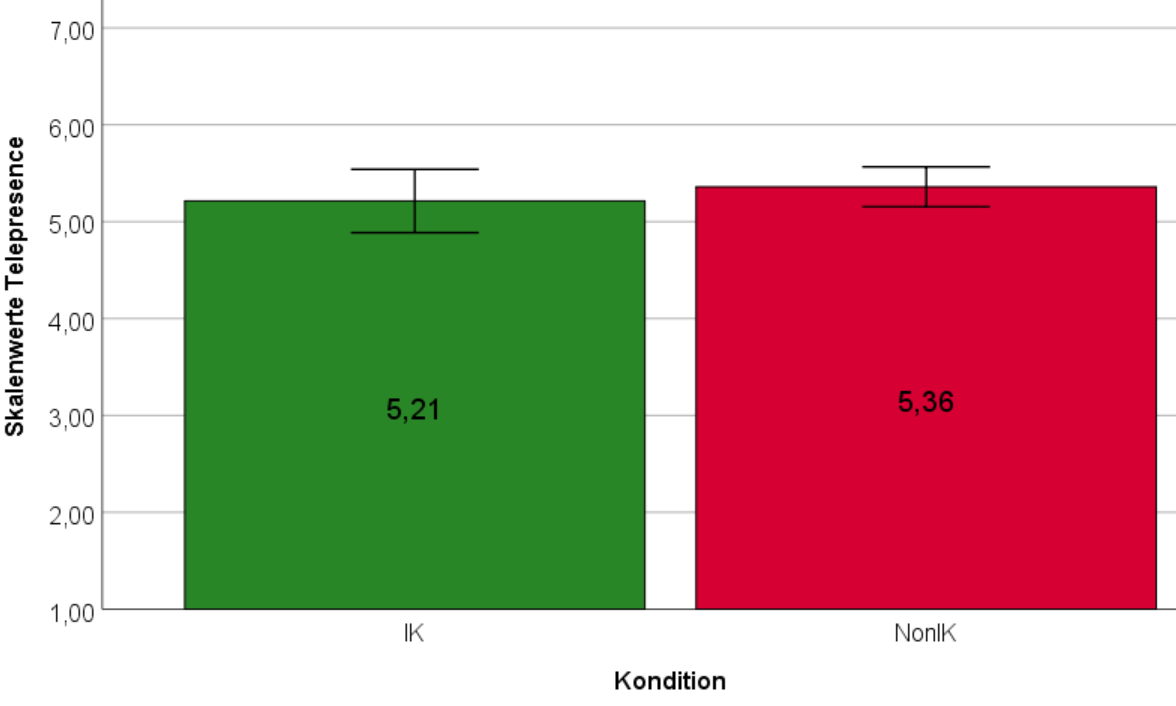
\includegraphics[width=\linewidth]{Abbildungen/AuswertungDiagramme/Final/SD_Telepresence_Mittelwerte.png}
      \caption[Durchschnittlich wahrgenommene Telepräsenz]{In dieser Abbildung werden die Mittelwerte der \textit{Telepräsenz} pro Kondition dargestellt. Der vertikale Fehler beschreibt den Standardfehler.}
       \label{SD_Telepresence_Mittelwerte}
   \end{minipage}
\end{figure}


\paragraph{Soziale Präsenz} 
Laut Kolmogoroff-Smirnov-Test ist die \textit{soziale Präsenz} mit $p =,031 < \alpha = ,05$ nicht normalverteilt. 
Sie beträgt bei der Kondition \ac{ik} im Mittel $\bar{x} = 6,314$ mit einer Standardabweichung von $\sigma = 1,883$ und
bei der Kondition \ac{nik} im Mittel $\bar{x} = 6,504$ mit einer Standardabweichung von $\sigma = 1,540$. 
Laut Mann-Whitney-U-Test gibt es \textbf{keinen signifikanten Unterschied} zwischen den Mittelwerten ($U = 111,000; Z = -,062; p =,950 > \alpha = ,05$) (siehe \textit{Abbildung \ref{BP_SocialPresence}} und \textit{Abbildung \ref{SD_SocialPresence_Mittelwerte}}).
	
		\begin{figure}[H]
   \begin{minipage}[t]{.5\linewidth} % [b] => Ausrichtung an \caption
      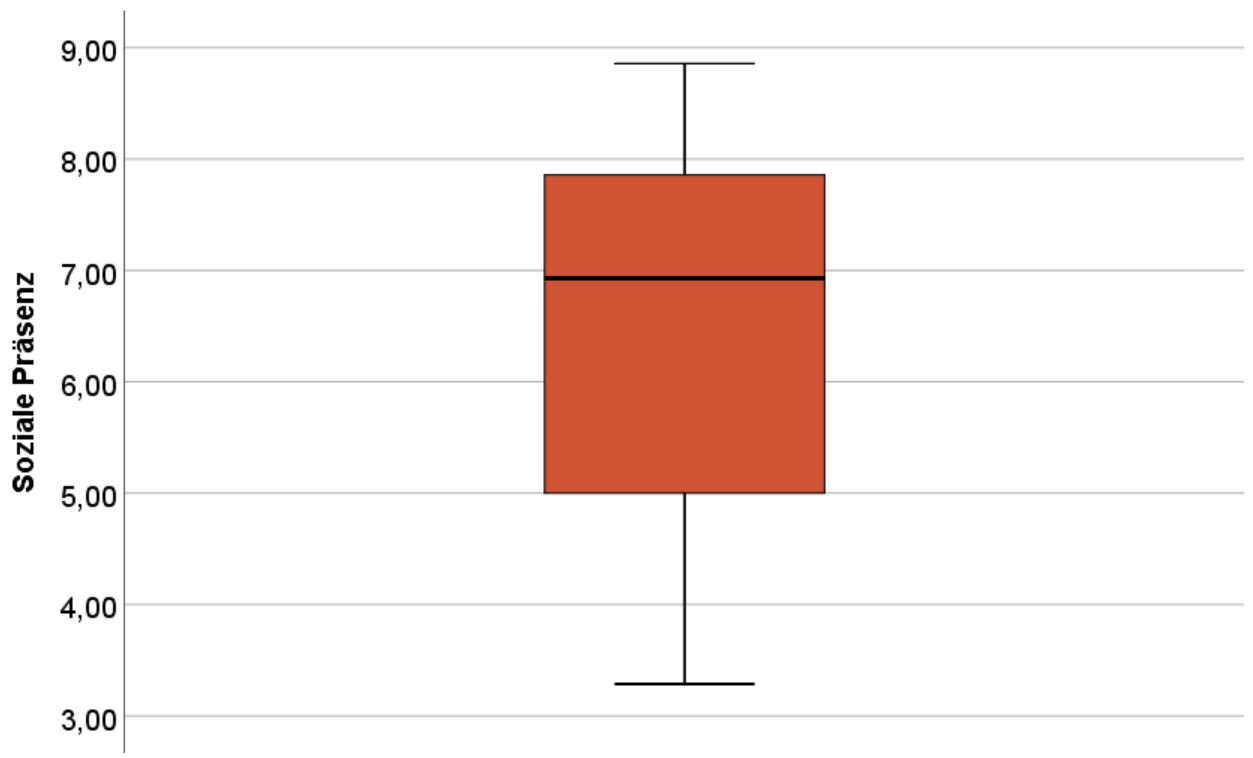
\includegraphics[width=\linewidth]{Abbildungen/AuswertungDiagramme/Final/BP_SocialPresence.png}
      \caption[Boxplot der gespürten sozialen Präsenz]{Diese Abbildung zeigt den Boxplot der gespürten \textit{sozialen Präsenz}.}
            \label{BP_SocialPresence}
   \end{minipage}
   \hspace{.02\linewidth}% Abstand zwischen Bilder
   \begin{minipage}[t]{.5\linewidth} % [b] => Ausrichtung an \caption
     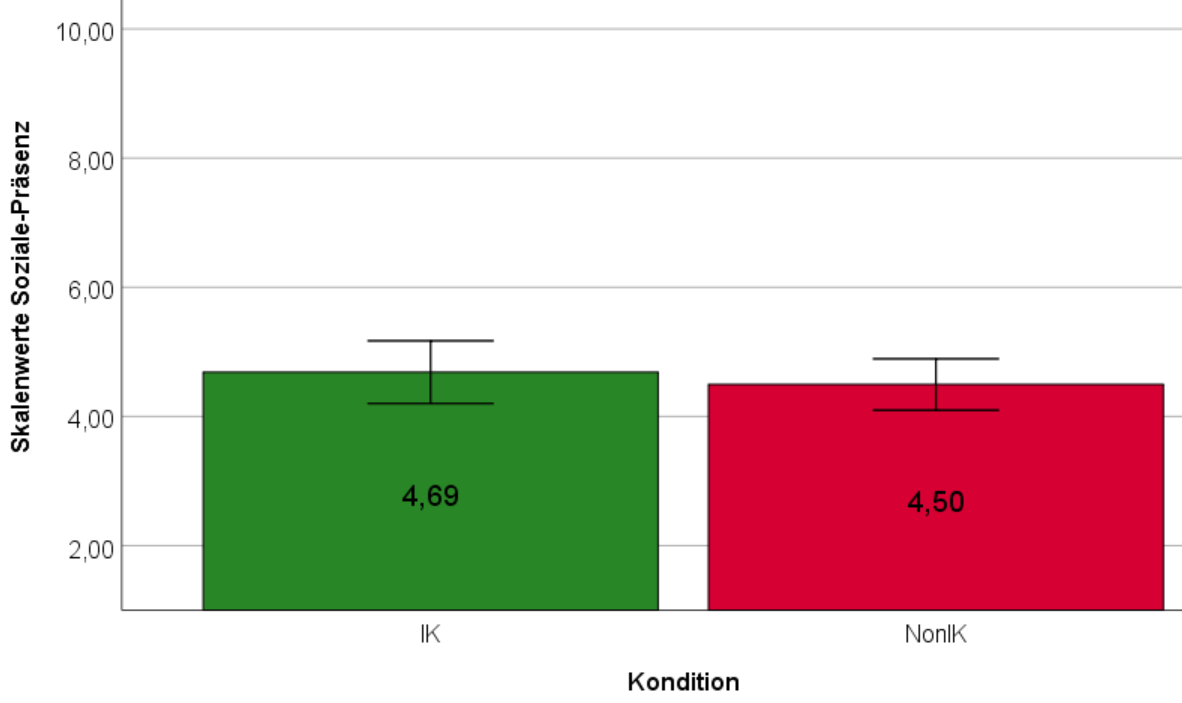
\includegraphics[width=\linewidth]{Abbildungen/AuswertungDiagramme/Final/SD_SocialPresence_Mittelwerte.png}
      \caption[Durchschnittliche soziale Präsenz]{Diese Abbildung zeigt den durchschnitt der \textit{sozialen Präsenz} der verschiedenen Konditionen. Der vertikale Fehler zeigt den Standardfehler.}
       \label{SD_SocialPresence_Mittelwerte}
   \end{minipage}
\end{figure}

\newpage

\paragraph{NASA-TLX \glqq{}empfundene Belastung\dq{}}
\label{NASA-TLX}
Die \textit{empfundene Belastung} ist laut  Kolmogoroff-Smirnov-Test mit $p =,076 > \alpha = ,05$ normalverteilt. 
Sie beträgt bei der Kondition \ac{ik} im Mittel $\bar{x} = 6,900$ mit einer Standardabweichung von $\sigma = 2,907$.
Für die Kondition \ac{nik} beträgt sie im Mittel $\bar{x} = 7,100$ mit einer Standardabweichung von $\sigma = 2,756$. 
Der T-Test für unabhängige Stichproben zeigt \textbf{keinen signifikanten Unterschied} zwischen den Mittelwerten ($t(28) = -,193; p =,848 > \alpha = ,05$) (siehe \textit{Abbildung \ref{BP_NTLX}} und \textit{Abbildung \ref{SD_NTLX_Mittelwerte}}).

	\begin{figure}[H]
   \begin{minipage}[t]{.5\linewidth} % [b] => Ausrichtung an \caption
      \includegraphics[width=\linewidth]{Abbildungen/AuswertungDiagramme/Final/BP_Anstrengungsmaß.png}
      \caption[Boxplot der empfundenen Arbeitsbelastung]{Diese Abbildung zeigt den Boxplot der Werte der durchschnittlich \textit{empfundenen Arbeitsbelastung}.}
            \label{BP_NTLX}
   \end{minipage}
   \hspace{.02\linewidth}% Abstand zwischen Bilder
   \begin{minipage}[t]{.5\linewidth} % [b] => Ausrichtung an \caption
     \includegraphics[width=\linewidth]{Abbildungen/AuswertungDiagramme/Final/SD_NTLX_Mittelwerte.png}
      \caption[Durchschnittlich empfundene Arbeitsbelastung]{Diese Abbildung zeigt die durchschnittlich \textit{empfundene Arbeitsbelastung} der unterschiedlichen Konditionen ermittelt durch den NASA-TLX. Der vertikale Fehler zeigt den Standardfehler.}
       \label{SD_NTLX_Mittelwerte}
   \end{minipage}
\end{figure}

\paragraph{Team-Kommunikation} 
Laut Kolmogoroff-Smirnov-Test ist die \textit{Team-Kommunikation} mit $p =,018 < \alpha = ,05$ nicht normalverteilt. 
Diese beträgt bei der Kondition \ac{ik} im Durchschnitt $\bar{x} = 4,013$ mit einer Standardabweichung von $\sigma =,665$.
Bei der Kondition \ac{nik} beträgt sie im Durchschnitt $\bar{x} = 4,48$ mit einer Standardabweichung von $\sigma =,476$. 
Laut Mann-Whitney-U-Test ist ein \textbf{signifikanter Unterschied} der Mittelwerte ($U = 63,500; Z = -2,062; p =,039 < \alpha = ,05$) vorhanden (siehe \textit{Abbildung \ref{SD_TeamkommunikationBP}} und \textit{Abbildung \ref{SD_Teamkommunikation_Mittelwerte}}).

	\begin{figure}[H]
   \begin{minipage}[t]{.5\linewidth} % [b] => Ausrichtung an \caption
      \includegraphics[width=\linewidth]{Abbildungen/AuswertungDiagramme/Final/BP_Teamkommunikation.png}
      \caption[Boxplot der Team-Kommunikation]{Boxplot der \textit{Team-Kommunikation}.}
            \label{SD_TeamkommunikationBP}
   \end{minipage}
   \hspace{.02\linewidth}% Abstand zwischen Bilder
   \begin{minipage}[t]{.5\linewidth} % [b] => Ausrichtung an \caption
     \includegraphics[width=\linewidth]{Abbildungen/AuswertungDiagramme/Final/SD_Teamkommunikation_Mittelwerte.png}
      \caption[Durchschnittliche Team-Kommunikation]{Diese Abbildung zeigt die durchschnittliche \textit{Team-Kommunikation} bei unterschiedlichen Konditionen. Der vertikale Fehler beschreibt den Standardfehler. $** : p < \alpha = ,05$}
       \label{SD_Teamkommunikation_Mittelwerte}
   \end{minipage}
\end{figure}

\newpage

\paragraph{Wahrgenommene Teameffektivität}
Die \textit{wahrgenommene Teameffektivität} ist laut Kolmogoroff-Smirnov-Test mit $p =,018 < \alpha = ,05$ nicht normalverteilt. 
Bei der Kondition \ac{ik} beträgt die \textit{wahrgenommene Teameffektivität} im Mittel $\bar{x} = 4,520$ mit einer Standardabweichung von $\sigma = 1,590$ und bei der Kondition \ac{nik} im Mittel $\bar{x} = 5,253$ mit einer Standardabweichung von $\sigma = 1,012$. 
Laut Mann-Whitney-U-Test ist \textbf{kein signifikanter Unterschied} zwischen den Mittelwerten ($U = 76,000; Z = -1,520; p =,128 > \alpha = ,05$) vorhanden  (siehe \textit{Abbildung \ref{SD_TeameffektivitätBP}} und \textit{Abbildung \ref{SD_Teameffektivität_Mittelwerte}}).

		\begin{figure}[H]
   \begin{minipage}[t]{.5\linewidth} % [b] => Ausrichtung an \caption
      \includegraphics[width=\linewidth]{Abbildungen/AuswertungDiagramme/Final/BP_Teameffektivität.png}
      \caption[Boxplot der wahrgenommenen Teameffektivität]{Boxplot der \textit{wahrgenommenen Teameffektivität}.}
            \label{SD_TeameffektivitätBP}
   \end{minipage}
   \hspace{.02\linewidth}% Abstand zwischen Bilder
   \begin{minipage}[t]{.5\linewidth} % [b] => Ausrichtung an \caption
     \includegraphics[width=\linewidth]{Abbildungen/AuswertungDiagramme/Final/SD_Teameffektivität_Mittelwerte.png}
      \caption[Durchschnittlich wahrgenommene Teameffektivität]{Diese Abbildung zeigt die \textit{subjektiv wahrgenommene Teameffektivität} der einzelnen Teilnehmer pro Kondition. Der vertikale Fehler beschreibt den Standardfehler.}
       \label{SD_Teameffektivität_Mittelwerte}
   \end{minipage}
\end{figure}

\begin{table}[H]
	\centering\footnotesize\setstretch{1.7}
	\caption[Signifikante Unterschiede der subjektiven Daten]{Diese Tabelle zeigt, ob unterschiedliche subjektive Daten signifikante Unterschiede zwischen den beiden Avatar-Konditionen zeigen.}
	\label{SubSigTab}
	\begin{tabularx}{\textwidth}{| X | X |} 
		\hline \textbf{Was wurde analysiert?} & \textbf{Signifikant?}  \\
		\hline 
		\textit{Präsenz}
		& keine signifikanten Unterschiede \\
		\hline 
		\textit{Selbst wahrgenommene Co-Präsenz} 
		& keine signifikanten Unterschiede \\	
		\hline 	
		\textit{Wahrgenommene Co-Präsenz des anderen }
		& keine signifikanten Unterschiede \\		
		\hline 	
		\textit{Telepräsenz }
		& keine signifikanten Unterschiede \\		
		\hline 	
		\textit{Soziale Präsenz}
		& keine signifikanten Unterschiede \\			
		\hline 	
		\textit{Empfundene Belastung }
		& keine signifikanten Unterschiede \\			
		\hline 	
		\textit{Teamkommunikation}
		& \textbf{signifikanter Unterschied} \\			
		\hline 	
		\textit{Wahrgenommene Teameffektivität}
		& keine signifikanten Unterschiede \\ \hline
	
	\end{tabularx}
\end{table}		

\newpage
\paragraph{Weitere Analysen des kognitiven Vertrauens}
\label{Weiter Analysen}
\paragraph{Kognitives Vertrauen und wahrgenommene Teameffektivität}
Auf Konditionsebene ist eine starke positive Korrelation (vgl. \citep{cohen2013statistical}) mit dem Spearman- Korrelationskoeffizient $r =,869$ zwischen den \textit{kognitiven Vertrauenswerten} und \textit{der wahrgenommenen Teameffektivität} der Kondition \ac{nik} zu erkennen. Die Spearman-Korrelation ist \textbf{signifikant} ($p =,000 < \alpha = ,05$) und ist in \textit{Abbildung \ref{SubSig1}} dargestellt.\\

\begin{figure}[h]
  \centering
  \subfloat[][]{\includegraphics[width=0.45\linewidth]{Abbildungen/AuswertungDiagramme/Final/SubSig1_CT_WTE_IK.png}}
  \qquad
  \subfloat[][]{\includegraphics[width=0.45\linewidth]{Abbildungen/AuswertungDiagramme/Final/SubSig1_CT_WTE_NIK_withStars.png}}
  \caption[Spearman-Korrelation kog. Vert. NIK und wahrg. Teameffektivität NIK]{Spearman-Korrelationen der \textit{kognitiven Vertrauenswerte} auf Konditionsebene mit der \textit{subjektiv wahrgenommenen Teameffektivität}. Links (a) für die Kondition \ac{ik} und rechts (b) für die Kondition \ac{nik}.}
  \label{SubSig1}
\end{figure}

\paragraph{Kognitives Vertrauen und  Team-Kommunikation}

Weiterhin ist eine positive Korrelation starken Effektes (vgl. \citep{cohen2013statistical}) mit dem Spearman- Korrelationskoeffizient $r =,676$ zwischen den \textit{kognitiven Vertrauenswerten} und der \textit{Team-Kommunikation} der Kondition \ac{nik} auf Konditionsebene zu erkennen. Die Spearman-Korrelation ist \textbf{signifikant} ($p =,006 < \alpha = ,05$) (siehe \textit{Abbildung \ref{SubSig2}})\\

\begin{figure}[h]
  \centering
  \subfloat[][]{\includegraphics[width=0.45\linewidth]{Abbildungen/AuswertungDiagramme/Final/SubSig2_CT_TC_IK.png}}
  \qquad
  \subfloat[][]{\includegraphics[width=0.45\linewidth]{Abbildungen/AuswertungDiagramme/Final/SubSig2_CT_TC_NIK_withStars.png}}
  \caption[Spearman-Korrelationen kog. Vertrauen NIK und Team-Kommunikation NIK]{Spearman-Korrelationen der \textit{kognitiven Vertrauenswerte} mit der \textit{wahrgenommenen Team-Kommunikation}. Links (a) für die Kondition \ac{ik} und rechts (b) für die Kondition \ac{nik}}
  \label{SubSig2}
\end{figure}


\clearpage
\newpage

\begin{table}[H]
	\centering\footnotesize\setstretch{0.8}
	\caption[Gemessene Variablen - Mittelwerte, Standardabweichungen (Teil 1)]{Variablen, Mittelwerte, Standardabweichungen und Anzahl der Teilnehmer}
	\label{MittelwerteUndCo}
	\begin{tabularx}{\textwidth}{p{5cm} | p{1cm} p{1.5cm} p{1.5cm} p{2cm} p{1cm} p{2cm}} 
		Was wurde gemessen? & Min/Max möglich & Erreicht Min/Max & Mittelwert & Std.Abweichung & $N$ \\
		\hline \\
		Genereller Hang zum Vertrauen  & $1/7$ & $3,6/6,4$ & $5,251$ & $,6125$ & $30$ \\ \\
		Kognitives Vertrauen  & $1/5$ & $2,5/5,00$ & $4,405$ & $,558$ & $30$ \\ \\
		Kognitives Vertrauen-IK  & $1/5$ & $2,50/5,00$ & $4,188$ & $,651$ & $15$ \\ \\
		Kognitives Vertrauen-NIK  & $1/5$ & $4,00/5,00$ & $4,622$ & $,347$ & $15$ \\ \\
		Team-Kommunikation & $1/5$ & $3/5$ & $4,246$ & $,616$ & $30$ \\ \\
		Team-Kommunikation-IK & $1/5$ & $3/5$ & $4,013$ & $,665$ & $15$ \\ \\
		Team-Kommunikation-NIK &$1/5$ & $3,4/5$ & $4,48$ & $,476$ & $15$ \\ \\
		Wahrg.Teameffektivität & $1/7$ & $1,00/7,00$ & $4,886$ & $1,362$ & $30$ \\ \\
		Wahrg.Teameffektivität-IK & $1/7$ & $1,00/7,00$ & $4,520$ & $1,590$ & $15$ \\ \\
		Wahrg.Teameffektivität-NIK  & $1/7$ & $3,2/6,8$ & $5,253$ & $1,012$ & $15$ \\ \\
		Allgemeine Anstrengung & $1/21$ &$2,33/11,67$ & $7,00$ & $2,785$ & $30$ \\ \\
		Allgemeine Anstrengung-IK & $1/21$ & $2,33/11,67$ & $6,900$ & $2,907$ & $15$ \\ \\
		Allgemeine Anstrengung-NIK & $1/21$ & $2,83/11,33$ & $7,100$ & $2,756$ & $15$ \\ \\
		Präsenz & $1/7$ & $1,57/6,29$ & $4,464$ & $,960$ & $30$ \\ \\
		Präsenz-IK  & $1/7$ & $1,57/5,50$ & $4,423$ & $1,024$ & $30$ \\ \\
		Präsenz-NIK  & $1/7$ & $2,64/6,29$ & $4,504$ & $,926$ & $30$ \\ \\
		Selbst - Co-Präsenz & $1/5$ & $2,00/5,00$ & $3,827$ & $,940$ & $30$ \\ \\
		Selbst - Co-Präsenz-IK  & $1/5$ & $2,17/5,00$ & $3,888$ & $,950$ & $15$ \\ \\
		Selbst - Co-Präsenz-NIK  & $1/5$ & $2,00/5,00$ & $3,766$ & $,959$ & $15$ \\ \\
		Co-Präsenz des anderen  & $1/5$ & $2,17/4,75$ & $3,877$ & $,633$ & $30$ \\ \\
		Co-Präsenz des anderen-IK  & $1/5$ & $3,08/4,75$ & $4,011$ & $,510$ & $15$ \\ \\
		Co-Präsenz des anderen-NIK  & $1/5$ & $2,17/4,67$ & $3,744$ & $,730$ & $15$ \\ \\
		Telepräsenz  & $1/7$ & $2,0/7,0$ & $5,286$ & $1,042$ & $30$ \\ \\
		Telepräsenz-IK  & $1/7$ & $2,0/7,0$ & $5,213$ & $1,265$ & $15$ \\ \\
		Telepräsenz-NIK  & $1/7$ & $3,4/6,8$ & $5,360$ & $,797$ & $15$ \\ \\
		Soziale Präsenz  & $1/10$ & $3,29/8,86$ & $6,409$ & $1,693$ & $30$ \\ \\
		Soziale Präsenz - IK  & $1/10$ & $3,57/8,86$ & $6,314$ & $1,883$ & $15$ \\ \\
		Soziale Präsenz - NIK  & $1/10$ & $3,29/8,14$ & $6,504$ & $1,540$ & $15$ \\ \\
	\end{tabularx}
\end{table}
\clearpage

\begin{table}[H]
	\centering\footnotesize\setstretch{0.8}
	\caption[Gemessene Variablen - Mittelwerte, Standardabweichungen (Teil 2)]{Variablen, Mittelwerte, Standardabweichungen und Anzahl der Teilnehmer}
	\label{MittelwerteUndCo2}
	\begin{tabularx}{\textwidth}{p{5cm} | p{1cm} p{1.5cm} p{1.5cm} p{2cm} p{1cm} p{2cm}} 
		Was wurde gemessen?  & Min/Max möglich &Erreicht Min/Max & Mittelwert & Std.Abweichung & $N$ \\
		\hline \\
		Teameffektivität im Team  &&$4/13$& $9$ & $2,666$ & $10$ \\ \\
		Teameffektivität im Team-IK && $4/13$ & $9$ & $3,535$ & $5$ \\ \\
		Teameffektivität im Team-NIK  && $7/12$ & $9$ & $1,870$ & $5$ \\ \\	
		Kognitives Vertrauen im Team  & $3/15$ & $11,67/14,83$ & $13,217$ & $1,151$ & $10$ \\ \\
		Kognitives Vertrauen im Team-IK  & $3/15$& $11,67/14,00$ & $12,56$ & $1,101$ & $5$ \\ \\
		Kognitives Vertrauen im Team-NIK  & $3/15$& $13,00/14,83$ & $13,866$ & $,845$ & $5$ \\ \\
		Generelles Vertrauen im Team & $3/21$& $14,60/17,45$ & $15,755$ & $1,009$ & $10$ \\ \\
		Generelles Vertrauen im Team-IK  & $3/21$& $14,60/16,75$ & $15,32$ & $,877$ & $5$ \\ \\
		Generelles Vertrauen im Team-NIK & $3/21$& $15,30/17,45$ & $16,19$ & $1,024$ & $5$ \\
	\end{tabularx}
\end{table}
\clearpage

%\subsection{Berechnung der Werte für die Auswertung}
%Bspw. Wie wurde CT oder GT etc. berechnet? UND WARUM BENÖTIGE ICH DIESE? WARUM Z.B. BESTANDENE TEAMRUNDEN ? -> WEIL NUR SO TEAMBUILDING ERFOLG GEMESSEN WERDEN KANN
%\newpage

\clearpage
\newpage
\section{Analyse}
Im Folgenden werden die statistisch ausgewerteten Hypothesen 1-5 sowie die subjektiv ausgewerteten Daten analysiert.
%Insgesamt zeigen die Ergebnisse Anzeichen dafür, dass unterschiedliche Avatar-Konditionen sich auf das gebildete kognitive Vertrauen der einzelnen Personen auswirkt. Es gibt jedoch keine Anzeichen dafür, dass es einen Zusammenhang zwischen kognitiven Vertrauen im Team oder generellen Vertrauen im Team und der Teameffektivität gibt. Weiterhin kann kein Unterschied der Avatar-Konditionen auf die Teameffektivität festgestellt werden.
%Die Ergebnisse zeigen kein Anzeichen dafür, dass unterschiedliche Avatar-Konditionen sich auf die Teameffektivität auswirken. 
%Es gibt keine Anzeichen dafür, dass es einen Zusammenhang zwischen dem generellem Vertrauen einer Person und dem gebildeten kognitiven Vertrauen einer Person gibt. 
%Es gibt ebenfalls keine Anzeichen dafür, dass der generelle Hang des Vertrauens im Team sich auf die Teameffektivität auswirkt. 
%Weiterhin gibt es keine Anzeichen dafür, dass sich das gemeinsame Vertrauen im Team sich auf die Teameffektivität eines Teams auswirkt.

\subsection{Analyse des kognitiven Vertrauens}
Es konnte ein \textit{signifikanter Unterschied} der Mittelwerte anhand eines durchgeführten Mann-Whitney-U Tests ($U = 64,000; Z = -2,029; p =,042 < \alpha =,05; r =-,370$) zwischen dem gebildeten \textit{kognitiven Vertrauenswerten}, bei unterschiedlichen Avatar- Konditionen, festgestellt werden. 
Die \textbf{Hypothese 1$_{1}$}, dass der erzielte \textit{kognitive Vertrauenswert} sich bei den Konditionen \ac{ik} und \ac{nik} \textit{signifikant} voneinander unterscheidet, wird angenommen. Es ist ein durchschnittlich höheres \textit{kognitives Vertrauen} bei der Kondition\newline \ac{nik} ($\bar{x}=4,622$) als bei der Kondition \ac{ik} ($\bar{x}= 4,188$) gebildet worden (siehe \nameref{Auswertung Hypothese 1}).\\

Durch die statistische Auswertung der \textbf{Hypothese 2} konnten \textit{keine signifikanten} Zusammenhänge anhand einer Spearman-Korrelation zwischen dem erzielten \textit{generellen Vertrauenswert} einer Person und dem erzielten \textit{kognitiven Vertrauenswert} einer Person, bei unterschiedlichen Avatar-Konditionen, festgestellt werden. Jedoch zeigt eine durchgeführte Fisher-Z-Transformation($Z =,954$) , dass sich die beiden Verteilungsformen der beiden Spearman-Korrelationen \textit{signifikant} voneinander unterscheiden ($p =,017 < \alpha =,05$) (siehe \nameref{Auswertung Hypothese 2}).\\
%Die beiden durchgeführten Spearman-Korrelationen korrelieren moderat positiv miteinander. 
Die Hypothese (H2$_{0}$), dass kein Zusammenhang zwischen dem erzieltem generellen Vertrauenswert einer Person und dem erzielten kognitiven Vertrauenswert bei unterschiedlichen Avatar-Konditionen besteht, wird angenommen.\\
Durch eine Analyse des Zusammenhangs zwischen dem \textit{kognitiven Vertrauen} und der \textit{wahrgenommenen Teameffektivität} auf Konditionsebene konnte ein \textit{signifikanter} positiver Zusammenhang bei der Kondition \ac{nik} festgestellt werden ($r =,869; p =,000 < \alpha = ,05$) .
Weiterhin konnte ein \textit{signifikanter} positiver Zusammenhang zwischen dem \textit{kognitiven Vertrauen} und der \textit{Teamkommunikation} auf Konditionsebene bei der Kondition \ac{nik} festgestellt werden ($r =,676; p =,006 < \alpha = ,05$) (siehe Kapitel \ref{Weiter Analysen}).

\subsection{Analyse der Teameffektivität}
\label{AnalyseTE}
Durch die statistische Auswertung der \textbf{Hypothese 3$_{0}$} konnte ein \textit{nicht signifikanter} schwach positiver Zusammenhang zwischen den \textit{kognitiven Vertrauenswerten der Teams} und der \textit{Teameffektivität der Teams} bei der Kondition \ac{ik} festgestellt werden ($r=,205 ;p =,741 > \alpha = ,05$)). Dieser Zusammenhang ist bei der Kondition \ac{nik} stark positiv und \textit{signifikant} ($r=,975$; $p =,005 < \alpha = ,05$). Die \textbf{Hypothese 3$_{1}$} kann somit nicht angenommen werden.\newline
Trotz dessen, dass die \textbf{Hypothese 3$_{1}$} nicht angenommen werden kann, wurde während der Analyse festgestellt, dass der Zusammenhang bei der Kondition \ac{nik} \textit{signifikant} und bei der Kondition \ac{ik} \textit{nicht signifikant} ist. Bekräftigt wird dieser \textit{signifikante} Zusammenhang der Kondition \ac{ik} dadurch, dass sich die beiden Verteilungsformen der Spearman-Korrelationen laut Fisher-Z-Transformation \textit{signifikant} voneinander unterscheiden ($Z=-1.977 ;p =,024 < \alpha = ,05$) (siehe \nameref{Auswertung Hypothese 3}).\newpage

Die Mittelwerte der \textit{Teameffektivität} bei unterschiedlichen Avatar-Konditionen sind identisch und unterscheiden sich laut Mann-Whitney-U ($U = 103,500; Z = -,377; p =,706 > \alpha = ,05; r = -,060$) \textit{nicht signifikant} voneinander. Die \textbf{Hypothese 4$_{1}$}, dass die \textit{Teameffektivität} sich bei unterschiedlichen Avatar-Konditionen signifikant voneinander unterscheidet, kann nicht angenommen werden. Die Nullhypothese (H4$_{0}$), die besagt, dass die Teameffektivität sich bei unterschiedlichen Avatar-Konditionen nicht signifikant unterscheidet, wird angenommen (siehe \nameref{Auswertung Hypothese 4}).\\

Die Analyse der \textbf{Hypothese 5$_{0}$} zeigt, dass \textit{keine signifikanten} Zusammenhänge der \textit{generellen Vertrauenswerte eines Teams} und der \textit{Teameffektivität eines Teams} bei unterschiedlichen Avatar-Konditionen bestehen. Da die Zusammenhänge nicht signifikant sind und die durchgeführte Fishers-Z-Transformation keine Unterschiede der Zusammenhänge aufzeigt, muss die Hypothese 5 {(H5$_{1}$) verworfen und die Nullhypothese (H5$_{0}$) angenommen werden. Diese besagt, dass der Zusammenhang zwischen dem \textit{generellen Vertrauenswert eines Teams} und der \textit{Teameffektivität eines Teams} mit der Kondition \ac{ik} sich nicht signifikant von den Teams mit der Kondition \ac{nik} unterscheidet (siehe \nameref{Auswertung Hypothese 5}).\\

Die Ergebnisse des NASA-TLX werden ebenfalls zur Analyse der \textit{Teameffektivität} hinzugezogen. Die empfundene Belastung der Teilnehmer mit den Konditionen \ac{ik} oder \newline \ac{nik} unterscheidet sich \textit{nicht signifikant} voneinander. Es kann in dieser Hinsicht folglich kein Vorteil bei einem der beiden Konditionen nachgewiesen werden (siehe \nameref{NASA-TLX}).
Auch hier kann der \textit{signifikante} positive Zusammenhang zwischen dem \textit{kognitiven Vertrauen} und der \textit{wahrgenommenen Teameffektivität} bei der Kondition \ac{nik} festgehalten werden.

\subsection{Analyse der subjektiven Daten}

Da nur bei einer Kategorie der subjektiven Daten signifikante Unterschiede zwischen beiden Konditionen festgestellt werden konnten, werden die übrigen Daten der Teilnehmer im Folgenden zusammen analysiert.

Anhand eines Mann-Whitney-U-Test konnte bei der Kategorie \textit{Teamkommunikation} ein \textit{signifikanter Unterschied} zwischen den Mittelwerten beider Avatar-Konditionen festgestellt werden (Mann-Whitney-U : $U = 63,500; Z = -2,062; p =,039 < \alpha = ,05$) . Der Mittelwert der \textit{Teamkommunikation} der Kondition \ac{ik} beträgt $\bar{x} = 4.013$, während der Mittelwert der Teamkommunikation der Kondition \ac{nik} $\bar{x} = 4,48$ beträgt. Somit ist die subjektiv empfundene Teamkommunikation bei der Kondition \ac{nik} signifikant höher als bei der Kondition \ac{ik} und bei beiden Konditionen ist die Tendenz einer hohen Teamkommunikation ersichtlich ($\bar{x} = 4,013$; $\bar{x} = 4,48$ $ > 3$).

Das von allen Teilnehmern durchschnittlich angegebene \textit{Gefühl der Präsenz} kann mit dem Wert $\bar{x} = 4,446$ als stark interpretiert werden ($\bar{x} > 3,5$). Die \textit{Telepräsenz} ($\bar{x} = 5,286$) sowie die \textit{soziale Präsenz} ($\bar{x} > 6,409$) werden etwas stärker als durchschnittlich empfunden und deuten dadurch auf ein höheres Gefühl der Anwesenheit sowie auf ein stärkeres Gefühl der Nähe zwischen den Teilnehmern hin. Auch die \textit{selbst wahrgenommene Co-Präsenz} sowie die \textit{wahrgenommene Co-Präsenz des anderen} liegen mit den Werten $\bar{x} = 3,827$ und $\bar{x} = 3,877$ über dem Mittelwert der Antwortmöglichkeiten ($\bar{x} > 2,5$) und weisen somit eine Tendenz zur starken \textit{Co-Präsenz} auf.

Daneben liegt die durchschnittlich \textit{wahrgenommene Teameffektivität} mit dem Wert $\bar{x} > 4,886$ über dem Wert 3,5 und lässt sich somit im Bereich der als eher stark empfundenen Teameffektivität ($3,5 - 7$) verorten.
Die Werte des NASA-TLX (Allg. Anstrengung) ($\bar{x} < 7$) zeigen, dass das VR Experiment als mittelmäßig bis wenig anstrengend wahrgenommen wurde ($\bar{x} < 11$ ).


\subsection{Analyse der technischen Anforderungen}

Schweizer et al. \citep[S. 270]{schweitzer2010conceptualizing} erläutern die 4 wichtigsten Kennzeichen eines \textit{virtuellen Teams} in der Literatur (siehe Kapitel \ref{AnforderungenLautSchweitzer}). Diese konnten in dieser Studie durch die entwickelte Versuchsumgebung erfüllt werden und das \ac{sve} bot folgende Eigenschaften:
\begin{itemize}
\item \textit{Zustandegekommen aufgrund von Kommunikationstechnologie.} Durch das \ac{hmd} sowie das genutzte Framework, konnte kommuniziert werden, Entscheidungen getroffen und Informationen ausgetauscht werden.
\item \textit{Räumlich getrennt} Durch die Online-Fähigkeit der entwickelten Versuchsumgebung, konnten die Teilnehmer von überall an dem Versuch teilnehmen.
\item \textit{Grenzübergreifend} Die Online-Fähigkeit erlaubte eine Zusammenarbeit von verschiedenen Regionen aus.
\item Asynchron. Die Teilnehmer haben nicht direkt asynchron an dieser Studie teilgenommen, jedoch, falls ein Teilnehmer die Versuchsumgebung verlassen hätte, hätten die anderen Versuchsteilnehmer mit ihrer aktuellen Aufgabe teilweise weiterarbeiten können.
\end{itemize}

Die technischen Anforderungen, die im Kapitel \textit{\ref{TechnischeAnforderungen}} aufgestellt werden, konnten hinreichend umgesetzt werden.
\begin{itemize}
\item \textbf{Online-Fähigkeit und Unterstützung mehrerer HMD's}: Durch das verwendete Framework \textit{Normcore} ist es mehreren Nutzern gleichzeitig möglich gewesen, von jedem beliebigen Ort an dem Experiment teilzunehmen. Die einzige Voraussetzung war, dass die Teilnehmer ein \ac{hmd}, einen Internetanschluss sowie einen Computer besitzen. Es ist somit möglich gewesen, die Anforderungen eines virtuellen Teams laut Schweitzer et al. \citep[S. 270]{schweitzer2010conceptualizing} (vgl. Kapitel \ref{AnforderungenLautSchweitzer}) zu erfüllen. 
\item \textbf{Geringe Latenz}: Es wurden zwei End-to-End Latenzmessungen durchgeführt. Die End-to-End Latenzmessung bezeichnet die Zeit, die benötigt wird, bis eine reale Aktion eines Nutzers von einem anderen Nutzer wahrgenommen wird. Die erste Latenzmessung betraf die Geschwindigkeit der Audioübertragung des Netzwerks. Es wurde eine durchschnittliche Latenz von \textbf{356ms} festgestellt.
Die zweite Messung betraf die Geschwindigkeit, in der die Avatare ihre Körperpositionen verändern. Dabei wurde eine durchschnittliche Geschwindigkeit von 294ms festgestellt.
Es wurden während des Experiments keine störende Bewegungsverzögerung und Audioübertragung wahrgenommen, weshalb die Anforderung als erfüllt angesehen wird.
\item \textbf{Steuerung und Verwaltung der Anwendung durch einen Spectator}: Durch einen eigenen Spectator-Client ist es möglich gewesen, die Anwendung von außen zu steuern und zu überwachen.
\item \textbf{Interaktionsmöglichkeiten}:  Durch das verwendete Framework \textit{Normcore} und dessen globalen Datenspeicher für unterschiedliche Variablen ist es möglich gewesen, alle Zustände und Informationen während der laufenden Versuchsdurchführung zwischen dem Client und Spectator zu synchronisieren. Durch das Nutzerfeedback wurde ebenfalls die intuitive Steuerung bestätigt.
\item \textbf{Sprachübertragung}: Die Implementierung eines RCP-basierten Netzwerkhandlings ermöglichte eine Sprachübertragung von Client zu Spectator und von Spectator zu Client.
\item \textbf{Avatar-Konditionen}: Der Spectator hatte bei dem verwendeten System die Möglichkeit, zur Laufzeit zwei verschiedene Avatar-Konditionen (\ac{ik} und \ac{nik}) für die Clients auszuwählen.
\end{itemize}
%
%Weiterhin besitzt das System noch \textbf{zusätzliche Anforderungen} :
%
%\begin{itemize}
%\item \textbf{Teamfähigkeit} Das Team muss eine Aufgabe gemeinsam lösen. Jedes Teammitglied muss zu gleichen Teilen involviert sein. Fehlt ein Teammitglied, soll die Aufgabe nicht lösbar sein.
%\item \textbf{Inkrementelle Erhöhung der Schwierigkeit} Um einen Vergleich zwischen der Teameffektivität herzustellen, mussten die Runden inkrementell schwieriger werden. Dies wurde dadurch gelöst, dass die Teilnehmer jede drei Runden ein Symbol mehr gestikulieren  oder erraten mussten.
%\item \textbf{Neutrale Avatare} Die Avatare sollen so neutral wie möglich gestaltet sein. 
%\item \textbf{Vermeidung von Bekanntheit} Um die gegenseitige Bekanntheit  Teilnehmer auszuschließen, wurde jedem Teilnehmer zu beginn des Versuchs ein Zufälliger Name zugeordnet. Vor dem gesamten Versuch konnten sich die Teilnehmer nicht sehen oder hören.
%Können die Teilnehmer sich vor dem Versuch gesehen, würde sich ein Kognitives-Vertrauen oder Kognitives-Misstrauen zu der anderen Person aufbauen. 
%Kennen sich die Personen untereinander schon, wirkt sich dies auf die Vertrauensbildung in der \ac{vr} in Form von schon vorhandenem Affektiven-Vertrauen auf die Ergebnisse aus.
%\item \textbf{Keine verbale Kommunikation} Da die Stimme der Teilnehmer ein Residuum ist, wurde die verbale Kommunikation von Versuchsteilnehmer zu Versuchsteilnehmer nicht gestattet. 
%\end{itemize}


\subsection{Zusammenfassung der Analyse}
%H1
Anhand der statistischen Analyse lässt sich feststellen, dass unterschiedliche Avatar-Konditionen einen \textit{signifikanten} Einfluss auf das gebildete \textit{kognitive Vertrauen} besitzen. Dabei haben Teilnehmer mit der Kondition \ac{nik} mehr \textit{kognitives Vertrauen gebildet} als Teilnehmer mit der Kondition \ac{ik}. 
%H3, H4
Es wurde zudem ein \textit{signifikanter} Zusammenhang zwischen dem gebildeten \textit{kognitiven Vertrauen im Team} und der \textit{Teameffektivität} bei der Kondition \ac{nik} festgestellt, jedoch unterscheidet sich die \textit{Teameffektivität} \textit{nicht signifikant} aufgrund unterschiedlicher Avatar-Konditionen voneinander.
%H5
Es gibt \textit{keine Anzeichen} dafür, dass es einen \textit{signifikanten} Zusammenhang zwischen dem \textit{generellen Vertrauen} und dem \textit{kognitiven Vertrauen} besteht. 
%H2
Weiterhin gibt es \textit{keine Anzeichen} dafür, dass es einen \textit{signifikanten} Zusammenhang zwischen dem \textit{generellen Vertrauen} oder dem \textit{generellen Vertrauen im Team} und der \textit{Teameffektivität} gibt.

Es wurde ein \textit{signifikanter} Unterschied der Mittelwerte der Teamkommunikation auf Konditionsebene festgestellt. Zudem kann festgehalten werden, dass sich ein erhöhtes Präsenz-Gefühl (Präsenz, Telepräsenz, selbst wahrgenommene Co-Präsenz, wahrgenommene Co-Präsenz des anderen und Soziale-Präsenz) auf Konditionsebene während der Versuchsdurchführung gebildet hat. Die allgemeine Belastung lag unter dem Durchschnitt der möglichen anzugebenden Werte und die wahrgenommene Teameffektivität war überdurchschnittlich hoch.
Weiterhin gibt es einen \textit{signifikant} positiven Zusammenhang zwischen dem \textit{kognitiven Vertrauen} und der \textit{wahrgenommenen Teameffektivität} und der \textit{Teamkommunikation} auf Konditionsebene bei der Kondition \ac{nik}.
Die technischen Anforderungen konnten hinreichend umgesetzt werden.
Eine Übersicht der Hypothesen und ob diese als signifikant bewertet werden, befindet sich in \textit{Tabelle \ref{SignifikanzOverview}}. Eine Tabelle der einzelnen Werte der Variablen befindet sich in \textit{Tabelle \ref{MittelwerteUndCo}}.

\begin{table}[H]
	\centering\footnotesize\setstretch{1.2}
	\caption[Annahme und Ablehnung der Hypothesen]{Diese Tabelle zeigt, ob eine Hypothese angenommen oder abgelehnt wurde.}
	\label{SignifikanzOverview}
	\begin{tabularx}{\textwidth}{| p{12cm} | p{3.5cm}} 
		Hypothese & Annahme  \\
		\hline \\
%		H1$_{0}$ : Ein hoher General-Trust-Score (\ac{gt}) wirkt sich \textbf{nicht positiv} auf den Cognitiven-Trust-Score (\ac{ct}) aus.\\
%\textbf{H1$_{1}$} : Der erzielte kognitive Vertrauenswert (\ac{ct}) unterscheidet sich bei den Konditionen \ac{ik} und \ac{nik} signifikant voneinander.\\ \\
%Alternative formulierung :
\textbf{H1$_{1}$}: Die Mittelwerte der erzielten kognitiven Vertrauenswerte unterscheiden sich bei den Konditionen \ac{ik} und \ac{nik} signifikant voneinander.\\
		& \textbf{angenommen} \\
		\hline \\
		
%		H2$_{0}$ : Die Konditionen \ac{ik} oder \ac{nik} haben \textbf{keinen signifikant abweichenden Einfluss} auf den Cognitive-Trust-Score (\ac{ct}). \\
%		\textbf{H2$_{1}$} : Es besteht ein Zusammenhang zwischen dem erzielten generellen Vertrauenswert \ac{gt} einer Person und dem erzielten kognitiven Vertrauenswert \ac{ct} einer Person.\\ \\
%		Alternative formulierung :
				\textbf{H2$_{1}$}: Je höher der erzielte generelle Vertrauenswert einer Person ist, desto höher ist der erzielte kognitive Vertrauenswert einer Person. \\
		& abgelehnt \\
		
		\hline 	\\	
%
%		\textbf{H3$_{1}$} : Der kognitive Vertrauenswert von Teams \ac{teamCog} korreliert mit der Teameffektivität von Teams \ac{tRound} und der Kondition \ac{ik} stärker als von Teams mit der Kondition \ac{nik}. \\ \\
%		H3a$_{0}$ : Ein hoher Cognitiver-Trust-Score hat \textbf{keinen Einfluss} auf die Teameffektivität (\ac{tRound}).
%Alternative Formulierung :
\textbf{H3$_{1}$}: Der Zusammenhang zwischen dem kognitiven Vertrauenswert von Teams und der Teameffektivität von Teams mit der Kondition \ac{ik} ist stärker als der von Teams mit der Kondition \ac{nik}. \\
		& abgelehnt \\		
		
		\hline 	\\	
%		\textbf{H4$_{1}$} : Die Teameffektivität \ac{tRound} unterscheidet sich bei den Konditionen \ac{ik} und \ac{nik} signifikant voneinander.\\ \\
%%		H4$_{0}$ : Die Konditionen \ac{ik} oder \ac{nik} haben \textbf{keinen signifikant abweichenden Einfluss} auf die Anzahl der erfolgreich abgeschlossenen Runden \ac{tRound} eines Teams.\\
%Alternative Formulierung :
		\textbf{H4$_{1}$}: Die Mittelwerte der Teameffektivität unterscheiden sich bei den Konditionen \ac{ik} und \ac{nik} signifikant voneinander.\\
		& abgelehnt\\

		\hline 	\\	
%		\textbf{H5$_{1}$} : Der generelle Vertrauenswert eines Teams \ac{teamGen} korreliert mit der Teameffektivität eines Teams \ac{tRound} und der Kondition \ac{ik} stärker als von Teams mit der Kondition \ac{nik}. \\ \\
%%		H5$_{0}$ : Teams, aufgeteilt nach Avatar Verkörperungen (\ac{ik}, \ac{nik}), mit einem hohem General-Trust-Score (\ac{gt}) \textbf{schließen nicht mehr Runden ab}, (\ac{tRound}) als die mit einem niedrigen General-Trust-Score \ac{gt}\\
%Alternative Formulierung :
			\textbf{H5$_{1}$}: Der Zusammenhang zwischen dem generellen Vertrauenswert eines Teams und der Teameffektivität eines Teams mit der Kondition \ac{ik} ist stärker als der von Teams mit der Kondition \ac{nik}. \\
		& abgelehnt \\
		
		\hline 	\\
		
%		H5a$_{0}$ : Teams mit einem hohem General-Trust-Score (\ac{gt}) erzielen \textbf{schließen nicht mehr Runden ab} (\ac{tRound} als die mit einem niedrigen General-Trust-Score \ac{gt}.\\		
%		& nicht signifikant \\
	\end{tabularx}
\end{table}		


\newpage
\section{Diskussion}

%	Was habe ich gemacht?
%	Was habe ich gefunden? 
%	Was bedeutet das genau?
%	
%Die Ergebnisse werden interpretiert und Erkenntnisse werden erläutert.
%
%Die Beschränkungen der Forschung und deren Auswirkungen werden dargelegt.
%
%Es wird beschrieben, inwiefern die Erwartungen erfüllt worden sind.
%
%Eventuelle Ursachen und Folgen für die Ergebnisse werden besprochen.
%
%Vorschläge für eventuelle weiterführende Forschungen werden gemacht.
%
%Ergebnisse werden interpretiert.
%
%Es werden keine zu vagen Empfehlungen für weiterführende Forschungen gemacht.
	

\paragraph{Allgemeines}
	Diese Studie trägt zum einen dazu bei, besser zu verstehen, welche Avatar- Konditionen in einem \ac{sve} zum Vertrauensaufbau eingesetzt werden sollten, und zum anderen, wie sich dort das gebildete Vertrauen auf die Effektivität eines Teams auswirkt. Mit Berücksichtigung des aktuellen Forschungsstandes wurde das kognitive Vertrauen der einzelnen Personen und des gesamten Teams sowie deren \textit{Teameffektivität} gemessen. Insgesamt wird eine der fünf aufgestellten Hypothesen dieser Arbeit angenommen.


%DAS NOCH IRGENDWO EINFÜGEN?
%Die Stichprobengröße betrug in dem Experiment $N = 30$, wobei, um Unterschiede und Zusammenhänge aufgeteilt nach Avatar-Konditionen festzustellen, diese Stichprobengröße auf $N = 15$ halbiert werden musste. Um Teameffekte zu messen, wurde das Team als Einheit gemessen. Dies führt dazu, dass bei $N = 5$ Teams mit der Kondition \ac{ik} und $N = 5$ Teams mit der Kondition \ac{nik} Zusammenhänge und Unterschiede gemessen werden konnten. 


%Hier auf größe der Stichprobe eingehen. 
%Hier auf die Hauptfaktoren eingehen, weshalb die Hypothesen nicht signifikant wurden
%	-3er Teams zu groß
%	-Dadurch, dass die Personen wussten, dass diese mit 3 Lebendigen Personen arbeiten, wurde viel vertrauen gebildet
%	-Visualisierung der Avatare
%	-Komplexität der Aufgabe - Eventuell zu leicht? Eventuell nicht genügend Vertrauensaufbau vorhanden? Vertrauensaufbau eher im Sinne von "Wenn mein Team Versagt, dann Leite ich das Versagen auf mein gesamtes Team ab" "Wenn mein Team gut ist, dann denke ich, dass mein Team sehr Zuverlässig ist.


%Der Titel dieser Masterarbeit lässt sich in 2 Fragestellungen unterteilen :

%Ist die Avatar-Kondition \ac{ik} oder die Avatar-Kondition \ac{nik} effektiver um Vertrauen in einem \ac{sve} zu bilden?

%Weshalb gibt es keine Auswirkungen?
%Was hat der Versuchsaufbau mit den Ergebnissen zu tun?
%

%Wirkt sich das gebildete Vertrauen der verschiedenen Avatar-Konditionen auf die Effektivität eines virtuellen Teams aus?
%Wenn ja : Welche Avatar-Kondition ist effektiver?
%Wie viel effektiver ist eine Avatar-Konditione?
%Wenn nein : Woran liegt es, dass die Teams gleich effektiv sind?

\subsection{Vertrauensaufbau und Teameffektivität}
\paragraph{Vertrauensaufbau durch die Avatar-Konditionen}

Die Ergebnisse des Experiments widersprechen der Untersuchung von Bente et al. (vgl. Kapitel \ref{AvatarTrust}), die vermuten ließ, dass bei der Kondition \ac{ik} ein größerer \textit{kognitiver Vertrauensaufbau} stattfindet als bei der Kondition \ac{nik} (Hypothese 1). Es ist laut der statistischen Auswertung genau das Gegenteil der Fall, denn die Teilnehmer mit der Kondition \ac{nik} erzielen im Durchschnitt einen signifikant höheren kognitiven Vertrauenswert.
Ein Grund für dieses Ergebnis könnte sein, dass der verwendete \ac{ik}-Avatar vom \textit{Uncanny Valley Effekt} betroffen ist (vgl. Kapitel \ref{Uncanny-Valley-Effekt}). Der verwendete Avatar (\ac{ik}) führte in der Studie von Waldow et al. \citep{waldow2019investigating} bereits zu einem Gefühl von Unbehagen bei den Teilnehmern.
Weiterhin könnte die in diesem Experiment verwendete Inverse-Kinematik, die eventuell zu unnatürlichen Bewegungsabläufen führte, als fremdartig empfunden worden sein. Auch dadurch falsch interpretierte Gestikulation kann zu einem geringeren Vertrauensaufbau in das jeweilige Gegenüber geführt haben. Ein Teilnehmer (ID9) mit der Kondition \ac{ik} schrieb als Feedback dazu:
\begin{quote}
\glqq{}Es war eine spannende Erfahrung am VR-Experiment teilzunehmen und hat Spaß gemacht. Die
Personen waren mir nah, obwohl sie eindeutig unreal wirkten; Vertrauen war nichtsdestotrotz vorhanden.\dq{}
\end{quote}

Da es diesbezüglich von den Teilnehmern mit der anderen Kondition keine Rückmeldung gab, wird vermutet, dass die Simplizität der nicht-menschenähnlichen Avatar-Kondition in kurzer Zeit der Kolloboration angenommen werden kann.

\paragraph{Vertrauensaufbau durch das generelle Vertrauen}
Dass kein signifikanter Zusammenhang zwischen dem \textit{kognitiven Vertrauen} und dem \textit{generellen Vertrauen} bei unterschiedlichen Avatar- Konditionen besteht (Hypothese 2), kann auch als Vorteil gesehen werden.
So lässt sich vermuten, dass es während einer kurzfristigen Zusammenarbeit in einem \ac{sve} nicht von Relevanz ist, wie hoch oder niedrig das \textit{generelle Vertrauen} einer Person ist. 
Da nur die unterschiedlichen Avatar-Konditionen einen signifikanten Einfluss auf die Bildung des kognitiven Vertrauens besitzen, kann davon ausgegangen werden, dass das \textit{generelle Vertrauen} während einer Kennenlernphase eines virtuellen Teams keine größere Rolle spielt und isoliert betrachtet werden kann. Natürlich sollte in längerfristig bestehenden virtuellen Teams darauf geachtet werden, dass sich das generelle Vertrauen durch den Einfluss der kognitiven und der affektiven Komponente (vgl. Kapitel \ref{Vertrauen als Zustand-Label}) weiterhin zum Positiven entwickelt, um die Teameffektivität zu steigern (vgl. Kapitel \ref{Vertrauensforschung}).
%
%
%Die während der Analyse der Hypothese 1 wurde einen höheren Mittelwert der Kondition\newline \ac{nik} als bei der Kondition \ac{ik} festgestellt. Diese Feststellung über den Vertrauensaufbau unter Avataren widerspricht der Untersuchung von Bente und Rüggen (vgl. \textbf{\textit{ Kapitel \ref{AvatarTrust}}}). Die Kondition \ac{ik} sieht menschenähnlich aus, weshalb sich hätte vermuten lassen, dass bei dieser Kondition bei Teilnehmer ein größerer kognitiver Vertrauensaufbau stattfindet, als bei der Kondition \ac{nik}  (vgl. \textbf{\textit{Vertrauen und virtuelle Teams}}). Jedoch ist laut der statistischen Analyse genau das Gegenteil der Fall. Gründe für dieses Ergebnis könnte sein, dass der Avatar von dem \textit{Uncanny Valley} Effekt betroffen sind (vgl. \textbf{\textit{Uncanny-Valley}}). Schon in der Studie von Waldow \citep{waldow2019investigating} tendiert der in dieser Studie eingesetzte Avatar(\ac{ik}) zum Unbehagen, was durch den Uncanny-Valley Effekt zu Stande kommen kann. Weiterhin kann es sein, dass die Gestukulation, während des Versuchs nicht eindeutig von den Teilnehmer mit der Kondition \ac{ik} ausgewertet werden konnten. Die Inverse-Kinematik kann falsch interpretiert worden sein, oder es sind durch diese unnatürliche Bewegungsmuster der Avatare aufgetreten. Dadurch, dass die Avatare eventuell \glqq{}anders als normale Menschen\dq{} wahrgenommen wurden, konnte diesen eventuell nicht all zu viel Vertrauen zugesprochen werden.
%Eine teilnehmende Person (ID9) mit der Kondition \ac{ik} schrieb im Feedback Teil des Fragebogens dazu : \newline
%\glqq{}\textit{Es war eine spannende Erfahrung am VR-Experiment teilzunehmen und hat Spaß gemacht. Die Personen waren mir nah, obwohl sie eindeutig unreal wirkten; Vertrauen war nichtsdestotrotz vorhanden.}\dq{}
%Es wird vermutet, dass die Simplizität der nicht-menschenähnlichen Avatar-Darstellung einfacher angenommen werden kann.
%
%Dass kein signifikanter Zusammenhang des kognitiven Vertrauens mit dem generellem Vertrauen bei unterschiedlichen Avatar-Konditionen besteht, kann auch als positiver Effekt gesehen werden. 
%So lässt sich vermuten, dass es nicht von Relevanz ist, wie hoch oder niedrig das generelle Vertrauen einer Person im \ac{sve} ist. Dies ist auch im Zusammenhang mit der signifikant unterschiedlichen Bildung von kognitiven Vertrauen von Avatar-Konditionen zu betrachten. Dadurch, dass nur die unterschiedlichen Avatar-Konditionen einen signifikanten Einfluss auf die Bildung des kognitiven Vertrauens besitzen, kann davon ausgegangen werden, dass das generelle Vertrauen isoliert betrachtet werden kann und bei einer Kennenlernphase eines \ac{vt} keine größere Rolle spielt.
%%Weshalb könnte es keine Auswirkungen gegeben haben?
%
\paragraph{Vertrauen im Team und Teameffektivität}
%\paragraph{Hypothese 3, Hypothese 4 und Hypothese 5}

Die Analyse der Hypothese 4 zeigt, dass sich die Werte der \textit{Teameffektivität} bei den Avatar-Konditionen \ac{ik} und \ac{nik} \textit{nicht signifikant} voneinander unterscheiden. Dies spiegelt sich in der \textit{Teameffektivität} der Teams wider, denn bei beiden Teamkonditionen beträgt die durchschnittliche \textit{Teameffektivität} $x = 9$.
Die Hypothese 3, in der vermutet wurde, dass der Avatar mit der Kondition \ac{ik} mehr \textit{kognitives Vertrauen} aufbaut, muss ebenfalls abgelehnt werden. Jedoch wurde während der Analyse dieser Hypothese festgestellt, dass es einen \textit{signifikanten Zusammenhang} zwischen dem gebildeten \textit{kognitiven Vertrauen} und der \textit{Teameffektivität} der Kondition \ac{nik} gibt. Da die Hypothese 4 nicht angenommen werden kann, jedoch ein signifikanter Zusammenhang mit der Kondition \ac{nik} bei der Analyse der Hypothese 3 festgestellt wurde, muss vermutet werden, dass die Ergebnisse der Hypothese 3 und Hypothese 4 entweder zufälliger Natur sind oder die Messung der Teameffektivität verbessert werden muss.
%Weshalb gibt es diesen Zusammenhang, obwohl die Teameffektivitätswerte gleich sind?
Es lässt sich vermuten, dass zu einem gewissen Grad \textit{kognitives Vertrauen} durch eine hohe \textit{Teameffektivität} gebildet wird: 
\begin{quote}
\glqq{}[...]Ohne Sprache ist die Kommunikation mit den anderen schon sehr schwierig. Trotzdem fand ich interessant, dass die Aufgabe überhaupt zu bewältigen war, und tatsächlich nach den ersten Erfolgen auch das Vertrauen zu den anderen entstand, dass sie in der Lage sind, die Aufgabe zu bewältigen, zu kommunizieren und das Kommunizierte zu verstehen.\dq{} (Teilnehmer (ID20) mit der Kondition \ac{nik}) 
\end{quote}

Die kleine Stichprobengröße der Studie könnte zudem eine Ursache dafür sein, dass die Ergebnisse von Hypothese 3 und Hypothese 4 keine eindeutigen Ergebnisse liefern. Bei einer deutlich größeren Stichprobengröße könnte bei einer größeren Varianz der \textit{Teameffektivitätswerte} gegebenenfalls ein signifikanter Unterschied oder ein eindeutiger signifikanter Zusammenhang mit dem \textit{kognitiven Vertrauen} und der \textit{Teameffektivitätswerte}, festgestellt werden.

Die Teameffektivität könnte auch vom Bildungsstand der Teilnehmer beeinflusst worden sein. Da der Großteil der Teilnehmer (80\%) ein abgeschlossenen Studium besaßen, kann dies die \textit{Teameffektivitätswerte} beider Konditionen angenähert haben, weshalb beide Teams die Selbe durchschnittliche \textit{Teameffektivität} besitzen. Weiterhin zeigt sich aufgrund des hohen Bildungsstandes der Teams, dass die Gruppe bei diesem Attribut keine Homogenität besitzt. Jedoch bilden die Teams dieser Studie reale Teams besser als wenn die Teams unterschiedliche Bildungsniveaus besäßen. Teams in der Realität bestehen häufig aus Mitgliedern mit Selben Bildungsniveau.

%H5
Der Grund dafür, dass es keinen signifikanten Zusammenhang zwischen dem \textit{generellen Vertrauen} und der \textit{Teameffektivität} in dieser Studie gab, kann ebenfalls auf die vorherig erwähnte Verbesserung der Messung der Teameffekvität oder der kleinen Stichprobe zurückzuführen sein. Weiterhin kann vermutet werden, dass das \textit{generelle Vertrauen} keinen Einfluss auf die \textit{Teameffektivität} besitzt und ebenfalls isoliert betrachtet werden kann.

%TODO
%Weiterer Grund: Teilnehmer wussten, dass die anderen reale personen waren… 
%HIER NOCH HIN, DASS NASA TLX ZWAR NICHT SIGNIFIKANT UNTERSCHIEDLICH, JEDOCH ERHÖHTE WERTE AUFWEIST
%HIER NOCH HIN, DASS WAHRGENOMMENE TE ZWAR NICHT SIGNIFIKANT UNTERSCHIEDLICH, JEDOCH ERHÖHTE WERTE AUFWEIST
%HIER NOCH HIN, DASS ES BEI KOG. VERT UND WAHRG. TE BEI NIK EINEN SIGNIFIKANTEN ZUSAMMENHANG GIBT. ALLES LAUT \label{TEinVT}
%HIER NOCH HIN : NASA-TLX: kein Unterschied bei den avatarkonditionen bedeutet, dass die avatare die empfundene belastung während des experiments nicht beeinflusst.




%Während der Analyse der Hypothese 4 wurde festgestellt, dass kein signifikanter Unterschied der Teameffektivität bei unterschiedlichen Avatar-Konditionen besteht. Dies spiegelt sich auch in der Teameffektivität der Teams wieder. Bei beiden Teams ist die durchschnittliche Teameffektivität $x=9$.  
%Ein Team bestand aus 3 Personen, was die Stichprobengröße verkleinerte. Somit nahmen 10 Teams mit insgesamt 30 Personen an dem Versuch teilnahmen. Diese Stichprobe ist sehr klein und könnte eine mögliche Ursache dafür sein, dass in Hypothese 3 und 5 keine signifikanten Ergebnisse erzielt wurden.
%
%Diese ähnlichen Teameffektivitäte wirken sich ebenfalls auf Hypothese 3 aus. Durch ähnliche Teameffektivitätswerte konnte kein Zusammenhang zwischen diesen und dem kognitiven Vertrauen festgestellt werden. 
%Auch wenn kein Zusammenhang des kognitiven Vertrauens und der Teameffektivität vorliegt, lässt sich vermuten, dass nichts desto trotz zu einem bestimmten Grad kognitives Vertrauen durch eine erhöhte Teameffektivität gebildet wird.
%Eine teilnehmende Person (ID20) mit der Kondition \ac{nik} schrieb dazu : \newline
%\glqq{}\textit{[...]Ohne Sprache ist die Kommunikation mit den anderen schon sehr schwierig. Trotzdem fand ich interessant, dass die Aufgabe überhaupt zu bewältigen war, und tatsächlich nach den ersten Erfolgen auch das Vertrauen zu den anderen entstand, dass sie in der Lage sind, die Aufgabe zu bewältigen, zu kommunizieren und das kommunizierte zu verstehen.}\dq{}
%Ebenso kann es sein, dass das Messverfahren (vgl. \textit{\ref{Schwierigkeit des Experiments}} mehr Varianzen der Teameffektivitätswerte hätte erzeugen müssen, um eine genauere Aussagen treffen zu können.
%Um die jedoch zu validieren, hätten mehr Teams an diesem Experiment teilnehmen müssen.
	
%\paragraph{Einfluss des Experiments auf die Ergebnisse}
%
%Nochmal revué passieren lassen, ob das Teamwork-Spiel das richtige war. Hätte ich vielleicht etwas ändern können am Aufbau? Eventuell ein Social dillemma szenario? Hätte ich da eventuell validere informationen raus bekommejn?
%%Was hat der Versuchsaufbau mit den Ergebnissen zu tun?
%
%Rundenaufbau -> Werden schwerer
%Größere Stichproben der einzelnen Teams
%
%
%
%Hätten die Runden kürzer sein können um einen positiven Teameffekt zu messen?
%
%
%\paragraph{Diskussion der Hypothesen}
%
%Es könnte die gleiche Anzahl von abgeschlossenen Runden pro Team sein, weil :
%-Das Teambuilding game wie ich es aufgebaut habe war ein schlechtes Messinstrument
%-Game hat relativ wenig mit Vertrauen zu tun.
%
%Wie wäre das Spiel verlaufen, wenn nur 2 Avatare an dem Game teilgenommen hätten?
%Hätte sich was geändert? Was haben die aktuellen 3 Avatare für eine Auswirkungen und welche folgen hat dies auf die mögliche Teameffektivität und das gebildete Cognitive Vertrauen?
%
%-3er Teams -> So nahe an der Realität wie möglich. Daher aber eventuell auch generell höheres Vertrauensgefühl, da man die Arbeit "von sich abdrängen kann", da eigentlich immer nur die erklärende Person zur Zeit unter druck steht.
%
%\subsection{Einfluss der subjektiven Daten}
%
%Keine Signifikanz von Social presence und co präsenz kann daher kommen, weil die testpersonen die ganze zeit miteinander interagiert haben. daher haben sich beide gruppen stark drin gefühlt oder stark dass der andere da ist
%Abh var : tRoundsIK mit unabh general-Trust score scheint Kubisch oder quadratisch
%
%Die subjektiven Daten alle in verbindung mit der Teambuldingmaßnahme setzen. Anstrengungsmaß z.B., weil man die Leute erst kennenlernen muss etc.
%
%Hürde : Fehlinterpretation der Gestikulationen
%
%
%
%Diese Arbeit behandelt XY nicht … .
%Es würde über den Rahmen dieser Arbeit hinausgehen, … .
%Es ist nicht das Ziel dieser Arbeit … .
%Die LeserInnen sollten beachten, dass diese Arbeit auf … basiert.
%Begrenzungen ergaben sich beim Durchführen der Interviews, da … .
%Eine Limitation der Bachelorarbeit ist zum einen … .
%Weiterer Forschungsbedarf ergibt sich aus … .
%
%Wo waren die Grenzen der Forschung?
%Habe ich bestimmte Limitiationen stark zu spüren bekommen?
%Sind Fragen offen geblieben?
%Was kann ich auf Basis meiner Resultate für zukünftige Forschungen empfehlen?
%
%
%Halte ebenfalls fest, inwiefern deine Resultate neue oder andere Erkenntnisse in Bezug auf dein Thema mit sich bringen. Gehe alle Möglichkeiten durch: Was genau hast du herausgefunden?
%
%Zukünftige Forschung über Kommunikationsmethoden und dem gebildeten Vertrauen.
%
%Social Identity und Teambuilding - Ein Avatar ist anders.
%
%Durch die Symbole ist das Experiment auch änderübergreifend einsetzbar gewesen.. pr eund post questionnaire haben das jedoch vehindert, da deutsch

\subsection{Avatar-Konditionen und Präsenz}
\paragraph{Avatar-Konditionen}
Die Literatur ließ darauf schließen, dass die menschenähnlichere Avatar-Darstellung bessere Werte bei den verschiedenen Kategorien der Präsenz erzielen würde. Die statistische Auswertung zeigt jedoch, dass in diesem Experiment keine Unterschiede zwischen den Avatar-Konditionen \ac{ik} und \ac{nik} bei der selbst wahrgenommenen \textit{Co-Präsenz}, der \textit{Co-Präsenz} des anderen, der \textit{Telepräsenz} oder der \textit{Social-Präsenz} feststellbar sind. Die möglichen Gründe dafür sowie die qualitativen Daten der Befragung werden im Folgenden diskutiert.

\paragraph{Selbst-Avatar und Selbstpräsenz}
Keine der beiden Konditionen wurde als Selbst-Avatar dargestellt, sodass bei den Konditionen aus der Sicht eines Spielers lediglich die animierten Hände des eigenen Körpers zu sehen waren. 
%Laut X müssten die oben genannten Wahrnehmungsbereiche der Telepresence bei der Kondition IK – menschenähnlich besser bewertet werden. 
Dadurch, dass der sichtbare Anteil des eigenen Körpers in dieser Studie reduziert ist, kann das Ergebnis der Selbstpräsenz beider Avatar-Konditionen schlechter ausgefallen sein \citep[421-427]{construal2014connected}.
Die Avatar-Konditionen weisen zwar keinen Selbst-Avatar im klassischen Sinne auf, jedoch sind für den Spieler alle eigenen Körperteile abgebildet, die er aufgrund der Avatar-Darstellung der Mitspieler bei sich im eigenen Blickfeld vermutet (Hände). Dies kann erklären, weshalb die Selbstpräsenz beider Konditionen ähnlich stark empfunden wurden. Ein Teilnehmer (ID2) mit der Kondition \ac{ik} schrieb dazu:
\begin{quote}
\glqq{}Ich wusste nicht genau wie meine Arme zu sehen sind, ob ich ein[en] Buchstabe auch mit den Armen formen, statt mit den Händen schreiben konnte.\dq{}
\end{quote}
Diese Aussage lässt darauf schließen, dass die realere Avatar-Darstellung ohne einen passenden Selbst-Avatar für Verwirrung und Unsicherheit bei einigen Teilnehmern gesorgt hat. Das kann zu einem Break-in-Presence geführt haben, sodass der vermutete Vorteil einer realeren Avatar-Darstellung aufgehoben wurde. Hier muss jedoch erwähnt werden, dass ein Selbst-Avatar bei diesem Experiment wahrscheinlich ebenfalls für Verwirrung gesorgt hätte, da die Arme nicht getrackt wurden und sich somit nicht simultan und natürlich mit dem Spieler hätten mitbewegen können. Dadurch, dass allein die Hände angezeigt wurden, konnte sichergestellt werden, dass die Teilnehmer dazu tendieren, nur ihre Hände/Controller zum Kommunizieren zu verwenden (in der Erläuterung des Experiments wurde ebenfalls darauf verwiesen).

\paragraph{Co-Präsenz und Co-Präsenz des anderen} Da die Teilnehmer während und vor dem Experiment zudem wussten, dass sie mit weiteren \textit{realen} Personen zusammenarbeiten, fiel es ihnen vermutlich unabhängig von den Avatar-Konditionen leicht, sich eine reale Person hinter den Avataren der Mitspieler vorzustellen. Dies könnte ebenfalls das kognitive Vertrauen beeinflusst haben. Ein Proband (ID8) mit der Kondition \ac{ik} schrieb dazu:
\begin{quote}
\glqq{}Es war ein sehr interessantes Erlebnis. Ich bin gespannt zu [e]rfahren, wer die Teilnehmer waren.\dq{}
\end{quote}

\paragraph{Social-Präsenz} Als Kritik wurde die fehlende Geschlechterunterscheidung der Avatare angemerkt. So schrieb ein Teilnehmer (ID4) mit der Kondition \ac{ik} dazu:
\begin{quote}
\glqq{}Warum gab es keine Frauenfiguren? Das würde mehr Realität erzeugen.\dq{}
\end{quote}
Diese Anmerkung lässt vermuten, dass die Avatare der Kondition \ac{ik} zwar menschenähnlicher dargestellt sind als die anderen Avatare, dadurch jedoch ein größerer Spielraum für Kritik an dem Realitätsgrad der Darstellung entsteht.

%
%
%Ein Grund diesbezüglich könnte das fehlende Selbst-Avatar der einzelnen Nutzer sein. Dies erhöht Laut Biocca ebenfalls die Selbstpräsenz der Avatare \citep[421-427]{construal2014connected}.
%Eine teilnehmende Person (ID2) mit der Kondition \ac{ik} schrieb dazu : \\
%\glqq{}\textit{Ich wusste nicht genau wie meine Arme zu sehen sind, ob ich ein Buchstabe auch mit den Armen formen, statt mit den Händen schreiben konnte.}\dq{}\\
%Diese Verwirrung der fehlenden Selbstpräsenz, hatte eventuell einen Präsenzdefizit zur folge.
%Weiterhin hat sich die fehlende Geschlechtsunterscheidung der Avatare bei einigen Teilnehmer merklich gemacht. So schrieb die teilnehmende Person (ID4) mit der Kondition \ac{ik} dazu :\\
%\glqq{}\textit{Warum gab es keine Frauenfiguren? Das würde mehr Realität erzeugen}\dq{}.\\
%Die Ähnlichkeit der erzeugten Präsenzen zwischen den beiden Avatar-Kondition könnte zustande gekommen sein, da durch die Art des Aufbaus des Experiments in dieser Studie, bei einem neu zusammenarbeitendem Team im \ac{sve}, der einzige Interaktionskanal die Nonverbale Kommunikation war. Die einzige Möglichkeit mit den Interaktionspartnern zu Kommunizieren, war der Fokus auf die Gestikulation. Da die Teilnehmer während und vor dem Experiment zudem wussten, dass diese mit weiteren \glqq{}realen\dq{} Personen zusammenarbeiten, konnte sich eventuell leichter eine reale Person hinter dem Avatar vorgestellt werden, was die Ähnlichkeit der Präsenzmessungen erklären könnte. Dies könnte ebenfalls das kognitive Vertrauen beeinflusst haben.
%Eine Teilnehmende Person (ID8) mit der Kondition \ac{ik} schrieb dazu : \\ 
%Dazu schreibt ID8 (\ac{ik}) : \glqq{}\textit{Es war ein sehr interessantes Erlebnis. Ich bin gespannt zu Erfahren, wer die Teilnehmer waren}\dq{}\\
%
\subsection{Schwierigkeit des Experiments}
\label{Schwierigkeit des Experiments}

Es ist möglich, dass das Experiment nicht komplex genug aufgebaut war, um einen eindeutigen Zusammenhang zwischen der Vertrauensbildung und der \textit{Teameffektivität} zu messen. Dies geht besonders aus den statistisch nicht signifikanten Ergebnissen der Analyse der Hypothesen 3, 4 und 5 hervor. So schrieb ein Teilnehmer (ID17) mit der Avatar-Kondition \ac{nik} dazu:
\begin{quote}
\glqq{}Zu kurz - zu einfach - zu grau.\dq{}
\end{quote}
Ähnliches schrieb ein Proband (ID21) mit der Kondition \ac{nik}:
\begin{quote}
\glqq{}Schwierigkeitsgrad hätte noch stärker sein dürfen.\dq{}
\end{quote}
%Dadurch, dass kein Team die höchste programmierte Stufe erreichen konnte, kam kein Deckeneffekt zustande. Doch das Schwierigkeitsgrad des Experiments hätte beispielsweise schneller angehoben werden können, um eine größere Varianz der einzelnen Effektivitätswerte der Teams zu generieren. 
Die Runden des Experiments hätten eventuell schneller abgearbeitet werden sollen, um eine größere Varianz der Effektivitätswerte der Teams zu generieren. Die Varianz der erzielten \textit{Teameffektivität} könnte sich eventuell noch weiter erhöhen, wenn ein Team aus zwei statt aus drei Personen besteht. Einzelne Runden des Experiments würden schneller abgearbeitet werden und das gebildete \textit{kognitive Vertrauen} könnte in einem direkten Vergleich zweier Personen gemessen werden. Durch diese Art der Kollaboration würde allerdings der komplexe Charakter eines Drei-Personen-Teams verloren gehen.

Einige Teilnehmer fanden das Experiment zu einfach. Der geringe Schwierigkeitsgrad könnte schnell Lerneffekte durch Repetivität gefördert und damit die \textit{Teameffektivität} beeinflusst haben. Dies würde auch erklären, weshalb sich Teams beider Konditionen als überdurchschnittlich effektiv einschätzten.
Eine teilnehmende Person (ID7) mit der Kondition \ac{ik} schreibt zu den natürlichen Lerneffekten :
\begin{quote}
\glqq{}Am Anfang habe ich ein wenig Druck verspürt, die richtigen Zeichen zu geben. Als ich gesehen habe, dass es gut funktioniert, hat es sehr viel Spaß gemacht.\dq{}
\end{quote}
%
%Es ist möglich, dass das Experiment nicht komplex genug aufgebaut war, um einen Zusammenhang zwischen der Vertrauensbildung und der \textit{Teameffektivität} zu messen.
%Dies ging besonders durch die statistisch nicht signifikanten Ergebnisse der Analyse der Hypothese 3, 4 und 5 hervor. 
%So schrieb eine teilnehmende Person (ID17) mit der Kondition \ac{nik} dazu :\\
%\glqq{}\textit{Zu kurz - zu einfach - zu grau}\dq{} \\
%Ähnliches schrieb die die teilnehmende Person (ID21) mit der Kondition \ac{nik} : \\
%\glqq{}\textit{Schwierigkeitsgrad hätte noch stärker sein dürfen}\dq{} \\
%Die Runden des Experiments hätten eventuell schneller abgearbeitet werden können, um eine größere Varianz der einzelnen Effektivitätswerte der Teams zu generieren. 
%Diese Varianz der erzielten \textit{Teameffektivität} könnte sich noch weiter erhöhen, wenn ein Team aus zwei statt aus drei Personen besteht. Einzelne Runden des Experiments würden schneller abgearbeitet werden und das gebildete kognitive Vertrauen könnte in einem direktem Vergleich gemessen werden.
%Durch diese Art des Kollaboration wäre allerdings der komplexe Charakter eines drei Personen Teams verloren gegangen.\newline
%Durch diese empfundene Einfachheit einzelner Teilnehmer könnten innerhalb eines Teams auch schneller Lerneffekte durch Repetitivität entstanden sein, die die reale sowie die wahrgenommene Teameffektivität beeinflusst haben.
%Eine teilnehmende Person (ID7) mit der Kondition \ac{ik} schreibt zu den Natürliche Lerneffekten : \\
%\glqq{}\textit{Am Anfang habe ich ein wenig Druck verspürt, die richtigen Zeichen zu geben. Als ich gesehen habe, dass es gut funktioniert, hat es sehr viel Spaß gemacht.}\dq{} 
%


%Das hier erklären?
%\begin{figure}[H]
%		\begin{footnotesize}
%		\centering
%			\includegraphics[scale=0.4]{Abbildungen/RoundDifficultyVariant.JPG}
%			
%			\caption[Abbildung 1]{Die steigende Schwierigkeit der zu drückenden Knöpfe der einzelnen Runden}
%			\label{RoundDifficulty}
%		\end{footnotesize}
%	\end{figure}



\subsection{Limitierungen}
Als technische Limitation dieser Arbeit kann die eingesetzte Technik der Gestikulation aufgeführt werden. Während dem Experiment ist aufgefallen, dass die Teilnehmer mit der Kondition \ac{ik} mehr Kommunizieren wollten, als diese konnten. Die unterstützten \ac{hmd}s boten keine Möglichkeit, die Finger oder die gesamten Hände in der \ac{vr} abzubilden. Die Verständigung innerhalb des \ac{sve} kann durch den Einsatz von Finger- und Handtracking intensiviert werden, da verschiedene Gesten genauer wiedergegeben werden können. Das Finger- und Handtracking ist beispielsweise durch eine Oculus Quest oder Oculus Quest 2 möglich. Ein weiterer Aspekt, um die Menschenähnlichkeit und den Realismus bei der Avatar-Kondition \ac{ik} zu erhöhen, wäre der Einsatz von Mimik.
Eine weitere Limitierung dieser Untersuchung war, dass die Teilnehmer bevor das Experiment startete wussten, dass diese in einem \ac{sve} mit realen Personen agieren würden. 

Darüber hinaus ist der Avatar mit der Kondition \ac{ik} in dieser Studie nicht auf Menschenähnlichkeit, Realismus oder Ähnliches überprüft worden. 
Da sich diese Untersuchung hauptsächlich mit dem gebildeten \textit{kognitiven Vertrauen} und der daraus resultierenden \textit{Teameffektivität} beschäftigt, können keine Aussagen über den Einfluss verschiedener Avatar-Konditionen auf das \textit{affektive Vertrauen} einer Person getroffen werden. Um diesen Einfluss zu messen, müssten längerfristige Forschungen durchgeführt werden.


%
%Da sich diese Forschung hauptsächlich mit dem gebildeten kognitiven Vertrauen und der daraus resultierenden Teameffektivität beschäftigt, können keine Aussagen über den Einfluss verschiedener Avatar-Konditionen auf das generelle Vertrauen einer Person getroffen werden. Um diesen Einfluss zu Messen, müssten längerfristige Forschungen durchgeführt werden. 
%Eine weitere Limitierung dieser Forschung war es, dass die Teilnehmer bevor das Experiment startete wussten, dass diese in einem \ac{sve} mit 3 weiteren realen Personen arbeiten würden. Eine interessante Fragestellung wäre es nun, den Teilnehmer im vorherein nicht zu erzählen, dass die Personen real sind und anschließend das gebildete kognitive Vertrauen und die Effektivität im Team zu messen.

\subsection{Ausblick}
\ac{sve}s entwickeln sich aktuell sehr rasant. Die Coronapandemie hat gezeigt, dass virtuelle Kollaborationsmaßnahmen einen großen Einfluss auf Unternehmen weltweit haben. Es ist mehr Forschung darüber nötig, wie Teams effektiv in einem \ac{sve} zusammenarbeiten können.

Es könnte nicht nur untersucht werden, welche Art eines Avatars in einem \ac{sve} mehr Vertrauen schafft oder mehr \textit{Teameffektivität} erzeugt, sondern auch, wie die eingesetzte Sprache, die Mimik, die Gestik, die Größe, das Geschlecht oder der vorherige Bekanntheitsgrad der Personen sich auf das Vertrauen und die \textit{Teameffektivität} auswirkt.
Weiterhin könnte untersucht werden, wie die Art und Dauer der Nutzung des \ac{hmd}s, während ein Team zusammenarbeitet, sich auf das Vertrauen ins Team und die Teameffektivität auswirkt.

Eine Weiterführung dieser Studie könnte untersuchen, in welchem Maß sich der \textit{kognitive Vertrauensaufbau im Team} ändert, je nachdem, ob die Teilnehmer wissen, dass sie mit Menschen zusammenarbeiten oder nicht. Darüber hinaus wäre es interessant zu untersuchen, wie sehr sich der Unterschied zwischen einer verbalen und einer nonverbalen Kommunikation auf das gebildete Vertrauen im Team in einem \ac{sve} auswirkt.  
Weiterhin könnten ähnliche Studien durchgeführt werden, bei denen die einzelnen Runden der Kollaborationsaufgabe schneller hintereinander ausgeführt werden oder die Avatare ein anderes Aussehen besitzen.
%\paragraph{Diskussion der eingesetzten Methoden}
%\paragraph{Auswirkungen auf die Gegenwart}
%\paragraph{Vorschläge für zukünftige Untersuchungen}
%
%\paragraph{IDEEN}
%Warum sind die Ergebnisse so wie diese sind?
%Haben die Probanten während der Anwendung Stress verspürt?
%
%
%\paragraph{Was kann besser gemacht werden?}
\clearpage
\newpage
\section{Zusammenfassung}
Das Ziel dieser Studie war es, den Einfluss von zwei verschiedenen Avatar-Konditionen\newline (\ac{ik}, \ac{nik}) auf die Vertrauensbildung in ein Team und die daraus resultierende \textit{Teameffektivität} in einem Shared-Virtual-Environment zu untersuchen. 
Anhand eines aufgestellten Forschungsdesigns wurden detaillierte Untersuchungen durchgeführt, bei denen die Daten der Studienteilnehmer mithilfe von Fragebögen und einer für diese Studie entwickelten \ac{vr}-Anwendung erhoben und analysiert werden konnten.

Für das Experiment mussten zeitgleich jeweils drei, räumlich voneinander getrennte Teilnehmer als Team in einem \ac{sve} Aufgaben erledigen. Jedes Team bekam dabei eine von zwei Avatar-Konditionen zugeteilt. Während der Durchführung der gemeinsamen Aufgabe wurde die gemeinsame \textit{Teameffektivität} ermittelt. Die Fragebogenumfrage diente dazu, einen Einblick in das \textit{generelle Vertrauen} und das gebildete \textit{kognitive Vertrauen} sowie die \textit{wahrgenommene Teameffektivität}, die \textit{subjektiven Empfindungen} hinsichtlich der Arbeitsbelastung und das gebildete \textit{Gefühl von Präsenz} einer Person und des Teams zu bekommen.

Es konnte ein signifikanter Unterschied beim gebildeten \textit{kognitiven Vertrauen} zwischen den Avatar-Konditionen festgestellt werden, wobei sich mehr \textit{kognitives Vertrauen} bei den nicht- menschenähnlichen Avataren bildete. Es konnte jedoch kein statistisch signifikanter Unterschied zwischen den Avatar-Konditionen und der \textit{Teameffektivität} festgestellt werden. Weiterhin zeigen die Ergebnisse keinen signifikanten Zusammenhang zwischen dem \textit{generellen Vertrauen} und dem gebildeten \textit{kognitiven Vertrauen} einer Person. Zwischen dem \textit{kognitiven Vertrauen} und der \textit{Effektivität eines Teams} konnte ein signifikanter Zusammenhang bei der Kondition \ac{ik} festgestellt werden.

In einem virtuellen Team besitzt die Avatar-Kondition laut dieser Studie somit keinen eindeutigen Einfluss auf die \textit{Teameffektivität}. Es kann jedoch sinnvoll sein, den Avatar nicht zu menschenähnlich zu gestalten, um mehr \textit{kognitives Vertrauen} zu bilden.
%Es empfiehlt sich, diese Studie mit einer großen Stichprobe zu replizieren und die Einflüsse anders gestalteter Avatare zu untersuchen. 
Die Arbeit in einem virtuellen Team muss folglich nicht mit aufwendig gestalteten Avataren unterstützt werden. So können beispielsweise Unternehmen, die mit virtuellen Teams in einem Shared-Virtual-Environment arbeiten wollen, auf simple Avatar-Modelle zurückgreifen, um den Vertrauensaufbau im Team zu unterstützen.

%Welche Avatar-Kondition sollte man nutzen um frühzeitig Vertrauen zu bilden?
%Warum ist eine Avatar-Kondition effektiver?
%
%Steigern nun unterschiedliche Avatar-Konditionen die \textit{Teameffektivität}?
%Steigern unterschiedliche Avatar-Konditionen das kognitive Kognitive Vertrauen?
%Gibt es einen Zusammenhang zwischen generellem Vertrauen und der gebildeten \textit{Teameffektivität}?
%Gibt es einen Zusammenhang zwischen dem kognitiven Vertrauen und der gebildeten \textit{Teameffektivität}?
%Gibt es einen Zusammenhang zwischen dem generellen Vertrauen und dem gebildeten kognitiven Vertrauen der unterschiedlichen Avatar-Konditionen?
%
%Insgesamt nochmal auf die EFFEKTIVITÄT der Vertrauensbildung UND der Effektivität an sich eingehen.
%Auch auf virtuelle Teams eingehen ...! Wichtig!
\newpage

%\bibliographystyle{dcu}
\printbibliography
	\newpage
	\appendix	
\section*{Anhang}\markboth{Anhang}{Anhang}
\addcontentsline{toc}{section}{Anhang}
\renewcommand{\thesubsection}{\Alph{subsection}}
	\subsection{Pre-Questionnaire}
	\label{Pre-Questionnaire}
	
	\begin{figure}[H]
	\centering
		\begin{footnotesize}
			\includegraphics[scale=0.6]{Abbildungen/Fragebogen/Pre-Questionnaire/PQ1}\\
		\end{footnotesize}
	\end{figure}	
	
	\begin{figure}[H]
	\centering
		\begin{footnotesize}
			\includegraphics[scale=0.6]{Abbildungen/Fragebogen/Pre-Questionnaire/PQ2}\\
		\end{footnotesize}
	\end{figure}	
	
	\begin{figure}[H]
	\centering
		\begin{footnotesize}
			\includegraphics[scale=0.6]{Abbildungen/Fragebogen/Pre-Questionnaire/PQ3}\\
		\end{footnotesize}
	\end{figure}	
	
	\begin{figure}[H]
	\centering
		\begin{footnotesize}
			\includegraphics[scale=0.6]{Abbildungen/Fragebogen/Pre-Questionnaire/PQ4}\\
		\end{footnotesize}
	\end{figure}	
	
	\begin{figure}[H]
	\centering
		\begin{footnotesize}
			\includegraphics[scale=0.6]{Abbildungen/Fragebogen/Pre-Questionnaire/PQ5}\\
		\end{footnotesize}
	\end{figure}	
	
	\begin{figure}[H]
	\centering
		\begin{footnotesize}
			\includegraphics[scale=0.6]{Abbildungen/Fragebogen/Pre-Questionnaire/PQ6}\\
		\end{footnotesize}
	\end{figure}	
	
\subsection{Post-Questionnaire - Konditionsabfrage}
\label{Post-Questionnaire}
\label{Post-Questionnaire - Konditionsabfrage}

	\begin{figure}[H]
	\centering
		\begin{footnotesize}
			\includegraphics[scale=0.6]{Abbildungen/Fragebogen/Post-Questionnaire/PQM1}
		\end{footnotesize}
	\end{figure}	

\newpage

\subsection{Post-Questionnaire - Generelles Vertrauen}
\label{Post-Questionnaire - Generelles Vertrauen}

	\begin{figure}[H]
	\centering
		\begin{footnotesize}
			\includegraphics[scale=0.6]{Abbildungen/Fragebogen/Post-Questionnaire/PQG1}
		\end{footnotesize}
	\end{figure}	
	
	\begin{figure}[H]
	\centering
		\begin{footnotesize}
			\includegraphics[scale=0.6]{Abbildungen/Fragebogen/Post-Questionnaire/PQG2}
		\end{footnotesize}
	\end{figure}	
	
	\begin{figure}[H]
	\centering
		\begin{footnotesize}
			\includegraphics[scale=0.6]{Abbildungen/Fragebogen/Post-Questionnaire/PQG3}
		\end{footnotesize}
	\end{figure}	
	
	\begin{figure}[H]
	\centering
		\begin{footnotesize}
			\includegraphics[scale=0.6]{Abbildungen/Fragebogen/Post-Questionnaire/PQG4}
		\end{footnotesize}
	\end{figure}	

\newpage
\subsection{Post-Questionnaire - Kognitives Vertrauen}	
\label{Post-Questionnaire - Kognitives Vertrauen}	

	\begin{figure}[H]
	\centering
		\begin{footnotesize}
			\includegraphics[scale=0.6]{Abbildungen/Fragebogen/Post-Questionnaire/PQC1}
		\end{footnotesize}
	\end{figure}	
	
	\begin{figure}[H]
	\centering
		\begin{footnotesize}
			\includegraphics[scale=0.6]{Abbildungen/Fragebogen/Post-Questionnaire/PQC2}
		\end{footnotesize}
	\end{figure}	

\newpage
\subsection{Post-Questionnaire - Teamkommunikation}	
\label{Post-Questionnaire - Teamkommunikation}	

\begin{figure}[H]
	\centering
		\begin{footnotesize}
			\includegraphics[scale=0.4]{Abbildungen/Fragebogen/Post-Questionnaire/PQKQ1}
		\end{footnotesize}
	\end{figure}	

\newpage
\subsection{Post-Questionnaire - Team-Effektivität}	
\label{Post-Questionnaire - Team-Effektivität}	

	\begin{figure}[H]
	\centering
		\begin{footnotesize}
			\includegraphics[scale=0.6]{Abbildungen/Fragebogen/Post-Questionnaire/PQTE1}
		\end{footnotesize}
	\end{figure}	

\newpage
\subsection{Post-Questionnaire - NASA-TLX}
\label{Post-Questionnaire - NASA-TLX}

	\begin{figure}[H]
	\centering
		\begin{footnotesize}
			\includegraphics[scale=0.6]{Abbildungen/Fragebogen/Post-Questionnaire/PQTLX1}
		\end{footnotesize}
	\end{figure}	
	
	\begin{figure}[H]
	\centering
		\begin{footnotesize}
			\includegraphics[scale=0.6]{Abbildungen/Fragebogen/Post-Questionnaire/PQTLX2}
		\end{footnotesize}
	\end{figure}	
	
	\begin{figure}[H]
	\centering
		\begin{footnotesize}
			\includegraphics[scale=0.6]{Abbildungen/Fragebogen/Post-Questionnaire/PQTLX3}
		\end{footnotesize}
	\end{figure}	
	
	\begin{figure}[H]
	\centering
		\begin{footnotesize}
			\includegraphics[scale=0.6]{Abbildungen/Fragebogen/Post-Questionnaire/PQTLX4}
		\end{footnotesize}
	\end{figure}	
	
	\begin{figure}[H]
	\centering
		\begin{footnotesize}
			\includegraphics[scale=0.6]{Abbildungen/Fragebogen/Post-Questionnaire/PQTLX5}
		\end{footnotesize}
	\end{figure}	
	
	\begin{figure}[H]
	\centering
		\begin{footnotesize}
			\includegraphics[scale=0.6]{Abbildungen/Fragebogen/Post-Questionnaire/PQTLX6}
		\end{footnotesize}
	\end{figure}	

\newpage
\subsection{Post-Questionnaire - IPQ}
\label{Post-Questionnaire - IPQ}

	\begin{figure}[H]
	\centering
		\begin{footnotesize}
			\includegraphics[scale=0.6]{Abbildungen/Fragebogen/Post-Questionnaire/PQP1}
		\end{footnotesize}
	\end{figure}	
	
	\begin{figure}[H]
	\centering
		\begin{footnotesize}
			\includegraphics[scale=0.6]{Abbildungen/Fragebogen/Post-Questionnaire/PQP2}
		\end{footnotesize}
	\end{figure}	
	
	\begin{figure}[H]
	\centering
		\begin{footnotesize}
			\includegraphics[scale=0.6]{Abbildungen/Fragebogen/Post-Questionnaire/PQP3}
		\end{footnotesize}
	\end{figure}	

\newpage
\subsection{Post-Questionnaire - Co-Presence}			
\label{Post-Questionnaire - Co-Presence}		

	\begin{figure}[H]
	\centering
		\begin{footnotesize}
			\includegraphics[scale=0.6]{Abbildungen/Fragebogen/Post-Questionnaire/PQCP1}
		\end{footnotesize}
	\end{figure}	
	
	\begin{figure}[H]
	\centering
		\begin{footnotesize}
			\includegraphics[scale=0.6]{Abbildungen/Fragebogen/Post-Questionnaire/PQCP2}
		\end{footnotesize}
	\end{figure}	
	
	\begin{figure}[H]
	\centering
		\begin{footnotesize}
			\includegraphics[scale=0.6]{Abbildungen/Fragebogen/Post-Questionnaire/PQCP3}
		\end{footnotesize}
	\end{figure}	
	
	\begin{figure}[H]
	\centering
		\begin{footnotesize}
			\includegraphics[scale=0.6]{Abbildungen/Fragebogen/Post-Questionnaire/PQCP4}
		\end{footnotesize}
	\end{figure}	
	
	\begin{figure}[H]
	\centering
		\begin{footnotesize}
			\includegraphics[scale=0.6]{Abbildungen/Fragebogen/Post-Questionnaire/PQCP5}
		\end{footnotesize}
	\end{figure}	
	
	\begin{figure}[H]
	\centering
		\begin{footnotesize}
			\includegraphics[scale=0.6]{Abbildungen/Fragebogen/Post-Questionnaire/PQCP6}
		\end{footnotesize}
	\end{figure}	

\subsection{Elektronischer Anhang}
\label{Erklärvideo}
\paragraph{Erklärvideo}
[...]/Masterarbeit elektronischer Anhang/Masterarbeit\_Anleitung\_und\_Erklärung.mp4

\label{Programmcode}
\paragraph{Programmcode}
[...]/Masterarbeit elektronischer Anhang/Programmcode/Teambuilding\_Trust

\label{Statistische Auswertung}
[...]/Masterarbeit elektronischer Anhang/Antworten des User-Tests

\subsection{Weiteres}	
	
\begin{figure}[H]
		\begin{footnotesize}
			\includegraphics[scale=1]{Abbildungen/criteriaForVirtualTeams.JPG}
			\caption[Kriterien für virtuelle Teams]{Kriterien für virtuelle Teams von \citep[S. 27]{schweitzer2010conceptualizing}}
			\label{criteriaForVirtualTeams}
		\end{footnotesize}
	\end{figure}	
	
%	\begin{figure}[H]
%	\centering
%		\begin{footnotesize}
%			\includegraphics[scale=0.6]{Abbildungen/CouchEtAl_1996_TrustScale}\\
%			\caption[Abbildung 1]{Items of the Trust Inventory \citep[305-323]{couch1996assessment}}
%			\label{Trust-Inventory}
%		\end{footnotesize}
%	\end{figure}
	

\end{document}
